\documentclass[12pt,3p,authoryear,review]{elsarticle}
\usepackage{amsmath,amssymb,amsfonts,amsthm} % Mathepaket, Symbole und Schriftart
\usepackage{natbib} % Bibliography style
\usepackage{geometry} % Margins setting
\usepackage{graphicx} % Graphics inclusion
\usepackage{hyperref} % Automatic hyperref creation
\hypersetup{
    colorlinks,
    linkcolor={black},
    citecolor={blue!50!black},
    urlcolor={green!50!black}
}
\usepackage[nameinlink]{cleveref} % Use label in reference
\usepackage{threeparttable} % Allows tables with caption and note
\usepackage{tabularx} % More options for tables
\usepackage{arydshln} % Draw dash lines in tabular
\usepackage{xcolor} % Different font colors
\usepackage{ragged2e} % Font typeset
\usepackage[section]{placeins} % Set float within section
\usepackage{microtype} % Subliminal refinements towards typographical perfection
\usepackage[font=small,labelfont=bf]{caption} % Small and bold captions
\usepackage{subcaption} % Captions for subfigures
% Deletes Elsevier preprint in footnote
\usepackage{epstopdf}
\usepackage{lipsum}
\usepackage{setspace}
\usepackage{nicefrac} % Typeset fractions
\makeatletter
\def\ps@pprintTitle{%
 \let\@oddhead\@empty
 \let\@evenhead\@empty
 \def\@oddfoot{}%
 \let\@evenfoot\@oddfoot}
\makeatother
% Adds date on the top frontmatter
\patchcmd{\MaketitleBox}{\footnotesize\itshape\elsaddress\par\vskip36pt}{\footnotesize\itshape\elsaddress\par\parbox[b][36pt]{\linewidth}{\vfill\hfill\textnormal{\today}\hfill\null\vfill}}{}{}
\patchcmd{\pprintMaketitle}{\footnotesize\itshape\elsaddress\par\vskip36pt}{\footnotesize\itshape\elsaddress\par\parbox[b][36pt]{\linewidth}{\vfill\hfill\textnormal{\today}\hfill\null\vfill}}{}{}

\interfootnotelinepenalty=10000

\newtheorem{prop}{Proposition}
\newtheorem{corollary}{Corollary}
\newtheorem{lemma}{Lemma}

% ----------------------------------------------------------------------------
% BEGIN DOCUMENT
\begin{document}%
% FRONTMATTER
\begin{frontmatter}%
% PAPER TITLE
\title{Shopping Time and Frictional Goods Markets:\\Implications for the New-Keynesian Model}%
% AUTHOR
\author[1]{Konstantin Gantert\corref{cor1}\fnref{fn1}}%
\ead{k.gantert@tilburguniversity.edu}%
% FOOTNOTES
\cortext[cor1]{Corresponding author}%
\fntext[fn1]{I am thankful for detailed comments by Thomas Steger, Zeno Enders, Sjak Smulders, Gregor von Schweinitz, Dajana Xhani, Florian Sniekers, Has van Vlokhoven, Shubhdeep Deb, and Leonardo Urrutia. Further, I’d like to thank all participants of research seminars at Tilburg University, Leipzig University, and Augsburg University and participants of the conference session at EEA Conference 2025 for their helpful comments.}%
% AFFILIATION
\affiliation[1]{organization={Tilburg University, Department of Economics},
				addressline={PO Box 90153},
				postcode={5000LE},
				city={Tilburg},
				country={The Netherlands}}
% DATE
\date{\today}%
% ABSTRACT
\begin{abstract}%
	\begin{small}%
		\onehalfspacing%
		We extend the New-Keynesian (NK) model by introducing costly household search effort and imperfect goods-market matching. Shopping effort and available capacity enter a CES matching function, which endogenizes both the price elasticity of demand and capacity utilization. The framework nests the benchmark NK model and delivers two key dynamic channels. First, search-price growth creates an inflationary wedge in the Euler equation, making aggregate demand much less interest-sensitive: the effective Euler slope is up to ten times flatter than in the benchmark. Second, firms face a trade-off between price markups and capacity utilization which steepens the Phillips curve even after accounting for higher Rotemberg costs: the output-gap Phillips slope is about 12\% larger. The results highlight the importance of separating shopping time from home production as the sign of their impact changes. Quantitatively, monetary policy is less powerful, TFP shocks look more RBC-like, and the model reproduces procyclical search effort and capacity utilization. A trade-off emerges: matching utilization well can tilt the labor wedge toward procyclicality because the endogenous (countercyclical) demand elasticity offsets the textbook NK labor-demand channel. Search-driven shocks microfound cost-push dynamics which decreases the need for artifical shocks to the elasticity of intratemporal substitution.\par%
		\vspace{0.1in}%
	\end{small}%
\end{abstract}%
% KEYWORDS and JEL CODES
\begin{keyword}%
	Goods search-and-matching \sep endogenous price elasticity \sep capacity utilization \sep Euler equation slope \sep search-augmented Phillips curve \sep search-driven cost-push shocks%
	\JEL E21 \sep E22 \sep E31 \sep E32 \sep E52%
\end{keyword}%
\end{frontmatter}%
%--------------------------------------------------------------------------
% SETUP MAIN PART
%--------------------------------------------------------------------------
\newpage%
\setcounter{page}{1}% Rücksetzen des Seitenzahl-Zählers auf 1
%--------------------------------------------------------------------------
% 1. INTRODUCTION
%--------------------------------------------------------------------------
\section{Introduction}
%--------------------------------------------------------------------------
% Introduction to the Paper / Setting the Framework
The New-Keynesian (NK) model is the cornerstone of modern monetary economics analyzing the relationship between price setting, monetary policy, and the business cycle. It builds on the assumptions of sticky prices and monopolistic competition. However, NK models implicitly assume frictionless acquisition as households follow their demand schedule effortlessly. While prices might be set inefficiently over the business cycle, trading on the goods market is seamless and efficient. This contrasts with the data.\\%
% Shopping Time in the Data
According to the American Time-Use Survey, time spent shopping -- research, wait time, travel time, and the purchase process -- on any given day takes up to $41$ minutes. This is $15\%$--$30\%$ of time spent on home production. Shopping time increases with both individual and aggregate income which indicates that shopping for additional quantity dominates shopping for better prices as a motive of search. The aggregate income elasticity of shopping time is estimated between $1.1$ and $1.6$ and can be as large as $4$ for high income individuals. Time spent on acquiring information is negligible for this elasticity \citep{petrosky-nadeauShoppingTime2016}. Data on different goods market variables hints in the same direction. U.S. industry capacity utilization is procyclical with a mean of $84\%$ and a quarterly standard deviation of $1.54\%$, consumer durables show a $9\%$ stockout rate \citep{khanInventoriesBusinessCycle2007}, advertising expenses are procyclical with a mean share of $6\%$ of U.S. GDP \citep{hallCyclicalResponseAdvertising2012}, and a countercyclical inventory-sales ratio \citep{den2024role} indicates that consumption varies more than production. Together, these facts imply that shopping time is at least a weak substitute to ''supply-side inputs'' in creating trades on the goods market. Following \cite{bai2025demand}, we use shopping time as a proxy for broader search effort on the goods market.\\%
% Why this is important (anecdotal evidence)
Everyday examples foster intuition: a table at a restaurant may sit empty while diners queue, reflecting peak demand contrasts with underutilization during off-peak hours. A bakery might sell out of bread in the morning but face unsold inventory later. Car dealerships illustrate mismatches as buyers wait months for custom orders while used car prices soar due to shortages. Firms sift through numerous supplier proposals before selecting one. In light of procyclical shopping time and utilization data, we ask the following \emph{research question}:%
% RESEARCH QUESTION
%--------------------------------------------------------------------------
\begin{enumerate}%
	\item[] \emph{How does costly search effort and imperfect goods market matching influence time-allocation of households over the business cycle and thus the supply and demand channels of the New-Keynesian (NK) model?}%
\end{enumerate}%
% CONTRIBUTION / RESEARCH METHOD / MAIN FINDINGS
%--------------------------------------------------------------------------
% MODEL APPROACH AND DIFFERENCES
The starting point and benchmark of this paper is a NK model with sticky prices, sticky wages, and home production. Shopping time is allocated to home production and thus a substitute to market goods and a proxy for price search. We contribute to the literature by introducing goods market SaM to this model to separate shopping time from home production and allow for a procyclical role as matching input \citep{petrosky-nadeauShoppingTime2016}. We model available capacity as the second matching input \citep{michaillatAggregateDemandIdle2015,sun2024excess} -- in contrast to \cite{qiuProcyclicalProductivityNew2022} who use varieties -- and thus give available capacity a double role of productive matching input and capacity constraint. We find that the NK model with goods market SaM (NK-SaM) nests the benchmark model. Aggregate supply and demand are affected by the \emph{price elasticity of demand}\footnote{Throughout the paper, we refer to the price elasticity of demand as the ''price elasticity'' to save space.} and \emph{capacity utilization channels}. Their variation depends on the interplay of sticky prices, firm market power, search cost convexity, and the goods market structure. The model predicts a decrease in long-run real GDP driven by underutilization of lower production capacity.\\%
% IMPACT ON THE MODEL AND ITS CURVES
Over the business cycle, the price elasticity decreases in search prices\footnote{Search prices are defined as the marginal disutility of finding one good in units of the numeraire good.} inducing varying competition on the goods market. It is amplified by variation in capacity utilization if search effort is a productive matching input. Following \cite{barro2025old}, who cites goods market SaM as a promising way to reconcile Old- and New-Keynesian models, we focus on the analysis of the dynamic IS and NK Phillips curves highlighting the impact of goods market SaM on inflation and the output gap. We find that the slope of the output gap Phillips curve is \emph{$12\%$ steeper} compared to the benchmark model. The Euler equation slope is \emph{up to ten times flatter} as search price growth acts inflationary working through price elasticity growth and making monetary policy less effective. Both curves highlight the importance of modeling shopping time separate from home production as the implications for aggregate supply and demand show opposite signs.\\%
% SIMULATIONS
The simulated NK-SaM model -- taking general equilibrium effects into account -- confirms the findings from the slope analysis. Output gap variation decreases significantly and monetary policy is less effective as competition on the goods market varies in the price elasticity. Hence, the NK-SaM model resembles a real-business-cycle model albeit being set up and calibrated as a NK model. It is capable of matching shopping time data and producing significant (albeit too low) procyclical variation in capacity utilization. However, it overpredicts variation in the price elasticity and creates a procyclical labor wedge when matching the procyclical efficiency wedge. This pattern follows from the new \emph{price elasticity channel} dominating the \emph{labor demand channel} of the NK model. Cost-push shocks arise naturally from the demand side as search effort shocks create recessions with rising prices.\\%
% RELATED LITERATURE
%--------------------------------------------------------------------------
% NK and Home Production Literature
This paper builds on three literatures -- New-Keynesian (NK) models, home production, and goods market search-and-matching (SaM). The NK literature explains business cycle fluctuations in inflation and output with a dynamic IS equation and a NK Phillips curve \citep{yun1996nominal}. The framework is extended by sticky wages (\cite{ercegOptimalMonetaryPolicy2000}) and unemployment in a tractable way \citep{gali2011unemployment}. Medium-sized models \citep{christianoNominalRigiditiesDynamic2005,christianoDSGEModelsMonetary2010} add bells and whistles to match the data and give a more realistic account of business cycle fluctuations. The home production literature models consumption as a combination of goods and time spent \citep{becker1965theory} and thus features an intratemporal trade-off between market and home work amplifying labor market variation \citep{benhabibHomeworkMacroeconomicsHousehold1991,greenwoodAllocationCapitalTime1991}. Shopping time is often included in home work and decreases in income \citep{aguiar2013time}. Home production models are a parsimonious representation of price search. They explain U.S. data better than previous models \citep{mcgrattan1997equilibrium}. Applied to NK models, home production leads to a steeper dynamic IS curve and a flatter NK Phillips curve amplifying nominal frictions \citep{gnocchiHouseworkFiscalExpansions2016,lesterHomeProductionSticky2014,safonova2017home}.\\%
% Goods Market SaM Literature
The goods market SaM literature focuses on the interaction of search (costs) and prices. Seminal work on price search highlights the impact on price setting \citep{burdett1983equilibrium,diamondModelPriceAdjustment1971,diamondSearchStickyPrices1993}, the interaction with price adjustment costs \citep{benabou1988search,benabou1992inflation}, and the interaction with money \citep{diamond1984money,kiyotaki1993search,lagos2005unified,rocheteau2005money,shi1997divisible,shi1998search}. Matching functions connect individual decisions to market tightness and can produce multiple equilibria where sentiment matters \citep{diamond1982aggregate,diamond1989rational}. More recent literature shows how goods market tightness in a price search model directly affects labor market outcome \citep{kaplanShoppingExternalitiesSelffulfilling2016} and how the role of heterogeneity in search affects price dispersion and price elasticities \citep{nord2023shopping,pytka2024shopping}. Another recent branch of literature focuses on quantity instead of price search where goods market frictions amplify labor market variables \citep{lehmann2010search,michaillatAggregateDemandIdle2015,petrosky-nadeauMacroeconomicDynamicsModel2015,petrosky2021hosios}, the determinants of business cycle fluctuations shift to demand shocks \citep{bai2025demand}, and the functional form of search costs matters \citep{mathaSearchProductMarket2011}. 
Adding sticky prices, goods market SaM produces procyclical productivity following monetary policy shocks \citep{qiuProcyclicalProductivityNew2022}, a three-dimensional price-setting framework \citep{michaillat2024beveridgean}, and an inventory-sales ratio that increases in goods market tightness \citep{den2024role}. We see these three papers as complementary to ours as the first focuses on variety search, the second does not feature separate labor and goods markets, and the third focuses on inventories. Closely related are the literatures on customer capital \citep{drozdUnderstandingInternationalPrices2012,gilchrist2017inflation,gourio2014customer,paciello2019price} and on spatial frictions in NK models \citep{schmitt2025hotelling}.\\%
% Table of Contents 
%--------------------------------------------------------------------------
The rest of the paper is organized as follows. \Cref{sec:model} develops the model. \Cref{sec:steady_states} discusses the steady-state. \Cref{sec:dynamics} derives the goods market SaM channels -- \emph{endogenous price elasticity} and \emph{endogenous capacity utilization} -- in the linearized dynamic model explicitly. \Cref{sec:analysis} quantifies the impact of goods market SaM on the aggregate supply and demand slopes. \Cref{sec:simulations} shows simulations. \Cref{sec:conclusion} discusses the results and concludes.%
%--------------------------------------------------------------------------
% 2. MODEL
%--------------------------------------------------------------------------
%--------------------------------------------------------------------------
% Model Setup: Adding Search Effort and Goods Market Matching
%--------------------------------------------------------------------------
\section{Model Setup: Adding Search Effort and Goods Market Matching}\label{sec:model}%
The model is built on our benchmark model described as a combination of \cite{ercegOptimalMonetaryPolicy2000,gali2011unemployment,lesterHomeProductionSticky2014}. The novel feature of the paper is goods market search-and-matching (SaM) à la \cite{michaillatAggregateDemandIdle2015}. Inputs to goods market matching are household search effort and available production capacity following \cite{sun2024excess}. In contrast to the literature, variable search effort and capacity utilization are determined by the \cite{moenCompetitiveSearchEquilibrium1997}-\cite{rotembergMonopolisticPriceAdjustment1982} framework. It is defined by a trade-off between sticky prices and flexible search prices which are defined as the marginal disutility of search effort required to match one good and denominated in the numeraire good. Goods markets can feature excess demand or excess supply, reflected in goods market tightness.%
% Goods Markets Setup
%--------------------------------------------------------------------------
\subsection{Goods Markets Setup}%
% Novel feature - Markets approach
Households and firms meet on goods markets where costly household search effort and imperfect matching lead to excess demand or supply of goods, both in the steady-state and over the business cycle. Both states of the market are equilibrium outcomes, as marginal search costs are equalized to trade benefits. The goods market is segmented along a continuum $i \in (0,1)$ of differentiated goods, $T_t(i)$, as search is directed following \cite{moenCompetitiveSearchEquilibrium1997}. Households exert costly search effort, $H_{S,t}(i)$, for each variety \textit{i} and each firm \textit{i} supplies its idle production capacity, $S_t(i)$, of its unique variety \textit{i} to the market\footnote{This setup is along the lines of \cite{michaillatAggregateDemandIdle2015,sun2024excess} and in contrast to \cite{bai2025demand,qiuProcyclicalProductivityNew2022} where the number of firms enters the matching function.}. Each customer relationship trades one unit of one variety of the differentiated final good. Customer relationships for variety \textit{i} are given by%
\begin{align}\label{eq:goods_matching}%
 	T_t(i) \; = & \; \psi_{t} \left[\gamma_S H_{S,t}(i)^{\Gamma_S} + \left(1-\gamma_S\right) S_t(i)^{\Gamma_S}\right]^{\frac{1}{\Gamma_S}},%
\end{align}%
where $\psi_{t}>0$ is the matching efficiency symmetric across all markets which fluctuates following an exogenous shock. $0<\gamma_S \leq 1$ is the demand elasticity determining the impact of household search effort on goods market matching. $-\infty<\Gamma_S<1$ is the matching input elasticity of substitution. For $\Gamma_S \rightarrow 0$, the matching function converges to a Cobb-Douglas case. $\Gamma_S < 0$ identifies complements which become stronger as $\Gamma_S$ decreases. Those three parameters determine the \emph{search effort productivity} in the model. \emph{Goods market tightness} for variety \textit{i} is defined as demand relative to supply, $x_{t}(i) = \nicefrac{H_{S,t}(i)}{S_t(i)}$. It shows excess demand on a market for $x_t(i)>1$, vice-versa. The probability of a household to find a final good \textit{i} is given by $f_{t}(i) = \nicefrac{T_t(i)}{H_{S,t}(i)}$. The probability of a firm \textit{i} to sell a unit of its good is given by $q_{t}(i) = \nicefrac{T_t(i)}{S_t(i)}$. Here, it is equivalent to capacity utilization.%
% HOUSEHOLDS
%--------------------------------------------------------------------------
\subsection{Households}%
There are infinitely many households in this economy. The representative household has a continuum of members represented by the unit square and indexed by a pair $(j,k) \in [0,1] \times [0,1]$. \textit{j} identifies the type of labor a household member is specialized in and \textit{k} identifies the disutility of work for that household member given by $\mu_M k^{\nu_M}$ if the member is employed and zero otherwise. The representative household searches for market goods, supplies labor to market and home production, and consumes both market and home-produced goods. We follow \cite{gali2011unemployment} to aggregate labor disutility across employed and unemployed members of the household. The representative household maximizes their intertemporal utility
\begin{align*}%
 	\mathbb{U}_t(j) \; = \; \mathbb{E}_0 \sum_{t=0}^{\infty} \beta^t \left[ \frac{C_t(j)^{1-\sigma}-1}{1-\sigma} - \frac{\mu_{S,t} H_{S,t}(j)^{1+\nu_S}}{1+\nu_S} - \frac{\mu_H H_{H,t}(j)^{1+\nu_H}}{1+\nu_H} - \frac{\mu_M H_{M,t}(j)^{1+\nu_M}}{1+\nu_M} \right],%
\end{align*}%
by consuming a composite good, $C_t(j)$, and allocating time to search effort, $H_{S,t}(j) = \int_0^1 H_{S,t}(i,j) di$, home production, $H_{H,t}(j)$, and market production, $H_{M,t}(j)$, with $\mu_{S,t}, \mu_H, \mu_M > 0$ and $\nu_S, \nu_H, \nu_M \geq 0$. The disutility created by search effort constitutes a \emph{search cost}. $\mu_{S,t}$ varies exogenously, capturing shocks to search disutility. The discount factor is given by $0\leq\beta<1$ and risk-aversion by $\sigma>0$. The composite good is aggregated by a CES aggregator%
\begin{align}%
	C_t(j) \; = \; \left[ \gamma_H C_{H,t}(j)^{\Gamma_H} + \left(1-\gamma_H\right) C_{M,t}(j)^{\Gamma_H} \right]^{\frac{1}{\Gamma_H}},\label{eq:composite_consumption}
\end{align}%
with market goods, $C_{M,t}(j) = T_t(j)$, and home goods, $C_{H,t}(j) = H_{H,t}(j)$, where $0 \leq \gamma_H < 1$ and $-\infty < \Gamma_H \leq 1$. As there are infinitely many households, the variety \textit{i} market goods finding probability, $f_{t}(i)$, is exogenous to each household. The aggregate market composite good is determined by a \cite{dixitMonopolisticCompetitionOptimum1977} index%
\begin{align*}%
 	T_t(j) = \left( \int_0^1 T_t(i,j)^{\frac{\epsilon_t-1}{\epsilon_t}} di \right)^{\frac{\epsilon_t}{\epsilon_t-1}},%
\end{align*}%
where $1 \le \epsilon_t \le \infty$ is the elasticity of substitution between varieties. It varies following an exogenous shock \citep{ireland_technology_2004}. The intertemporal budget constraint is given by%
\begin{align*}%
 	B_t(j) = \left(1+r_{t-1}\right) B_{t-1}(j) + \left(1-c_{W,t}(j)\right) W_t H_{M,t}(j) - \int_0^1 P_t(i) T_t(i,j) di + \Pi_{F,t}(j),%
\end{align*}%
where $B_t(j)$ are one-period nominal bonds which pay a nominal interest rate, $r_t$. Labor income is given by $\left(1-c_{W,t}(j)\right) W_t H_{M,t}(j) di$, where $W_t$ is a nominal wage and $c_{W,t}(j)= \frac{\kappa_W}{2} \left( \frac{W_{t}(j)}{W_{t-1}(j)} - \pi_W \right)^2$ are nominal wage adjustment costs with $\kappa_W \geq 0$ and steady-state nominal wage inflation, $\pi_W$. Final good expenses are given by $\int_0^1 P_t(i) T_t(i,j) di$, where $P_t(i)$ is the price for final good \textit{i}. $\Pi_{F,t}(j)$ are firm dividends paid to the households by a mutual fund where each household owns an equal share.%
% LABOR UNIONS
%--------------------------------------------------------------------------
\subsection{Labor Unions}%
There is a labor union that aggregates specialized household labor and supplies it to each firm \textit{i}. The labor union maximizes its profits according to%
\begin{align*}%
	\Pi_{U,t} = \mathbb{E}_0 \sum_{t=0}^{\infty} \beta_{0,t} \left[ W_t \left( \int_0^1 H_{M,t}(i) di - \left( \int_0^1 H_{M,t}(j)^{\frac{\epsilon_W-1}{\epsilon_W}} dj \right)^{\frac{\epsilon_W}{\epsilon_W-1}} \right)   \right],%
\end{align*}%
where $H_{M,t}(i)$ is labor supplied to firm $i$ consisting of specialized household labor aggregated following \cite{dixitMonopolisticCompetitionOptimum1977} with $1\leq\epsilon_W\leq\infty$ determining its substitutability.% 
% FIRMS
%--------------------------------------------------------------------------
\subsection{Firms}%
There are infinitely many firms on the unit interval. Each firm produces a unique variety of the final good and supplies its idle production capacity, $S_t(i)$, to the goods market. It employs labor in a production capacity function, $\mathcal{Y}_{M,t}(i) = A_t H_{M,t}(i)$, where $A_t>0$ is an exogenous technology process. Each firm \textit{i} maximizes its profits by%
\begin{align*}%
 	\Pi_{F,t} \; = \; \mathbb{E}_0 \sum_{t=0}^{\infty} \beta_{0,t} \left[ P_t(i) T_t(i) - W_t H_{M,t}(i) \right],%
\end{align*}%
where $\beta_{0,t}$ is the stochastic discount factor of the firm\footnote{The period discount factor of the firm is equal to the household stochastic discount factor as all firms are owned by the household mutual fund.}. Idle production capacity is given by%
\begin{align}%
 	\left(1+c_{P,t}(i)\right) S_t(i) \; = & \; \mathcal{Y}_{M,t}(i),%
\end{align}%
where $c_{P,t}(i) = \frac{\kappa_P}{2} \left( \frac{P_{t}(i)}{P_{t-1}(i)} - \pi \right)^2$ are proportional convex \cite{rotembergMonopolisticPriceAdjustment1982} price adjustment costs\footnote{We use \cite{rotembergMonopolisticPriceAdjustment1982} price adjustment costs instead of the staggered price-setting framework of \cite{calvoStaggeredPricesUtilitymaximizing1983} to rule out strategic complementarities on the firm side. This assumption does not alter the results as the linearized versions of the resulting Phillips curves are symmetric in their reduced-form.} with $\kappa_P \geq 0$ and steady-state price inflation, $\pi$. Each firm has a monopoly over its variety \textit{i} of the final good. It jointly sets available production capacity, $S_t(i)$, and the goods price, $P_t(i)$, while anticipating household search effort to maximize its profits. The core of this \cite{moenCompetitiveSearchEquilibrium1997}-\cite{rotembergMonopolisticPriceAdjustment1982} framework is managing the trade-off between price markup and capacity utilization, $q_t(i)$. Additional search effort increases \emph{search costs} and thus decreases the price a household is willing to pay. However, additional search effort also increases the \emph{capacity utilization} and thus decreases marginal costs. Optimal firm decisions depend on the interaction of search frictions and monopoly power.%
% GENERAL EQUILIBRIUM
%--------------------------------------------------------------------------
\subsection{General Equilibrium}%
% Real GDP
The real gross domestic product is determined by aggregate trades of the final good, $Y_t = T_t$, which also acts as the numeraire. The central bank follows a \cite{taylorDiscretionPolicyRules1993}-type rule and sets the nominal interest rate according to%
\begin{align}\label{eq:Taylor_rule}%
	\frac{1+r_t}{1+r} \; = & \; \left( \frac{1+r_{t-1}}{1+r} \right)^{i_r} \left[ \left( \frac{1+\pi_t}{1+\pi} \right)^{i_\pi} \left( \frac{Y_t}{Y_{N,t}} \right)^{i_{Gap}} \right]^{1-i_r} M_t,%
\end{align}
where $\pi$ is a central bank target, $r$ is determined by the steady-state real interest rate, $Y_{N,t}$ is potential output given by the flexible price version of the model including goods market SaM, $i_r\geq0$ determines policy inertia, and $i_\pi, i_{Gap}\geq 0$ are policy coefficients. $M_t$ is a monetary policy shock. All exogenous shocks follow an AR(1) process given by $X_t = X^{1-\rho_X} X_{t-1}^{\rho_X} \varepsilon_{X,t}, \quad \varepsilon_{X,t} \sim \mathcal{N}(0,\,\sigma_X^{2})$ where $0\leq\rho_X<1$ is its autocorrelation, and $\varepsilon_{X,t}$ is a white noise random process around a normal distribution with zero mean and standard deviation $\sigma_X$.%
% CALIBRATION
%--------------------------------------------------------------------------
\subsection{Calibration}\label{sec:calibration}%
The model is calibrated to the U.S. economy between 1984 and 2019. Time is in quarters. Data is retrieved from \cite{fredDATA} and \cite{atusDATA} and summarized in \ref{sec:appendix_calibration}. Common parameters follow the literature, i.e. \cite{christianoDSGEModelsMonetary2010} and \cite{gnocchiHouseworkFiscalExpansions2016}. An overview is given in \cref{tab:calibration}.\\%
% Overview table calibration
\begin{table}%
	\begin{center}%
	\begin{footnotesize}%
	\caption{Overview of the Model Default Calibration}\label{tab:calibration}%
	\begin{tabular}{l c@{\hskip 18pt} l c @{\hskip 18pt} l c}%
		\hline%
		Parameter & Value & Parameter & Value & Parameter & Value\\%
		\hline \hline%
		$\beta$ & $0.99$ & $\psi$ & $\bar{cu}=0.86$ & $\sigma_A$ & $0.0064$\\%
		$\sigma$ & $1.5$ & $\gamma_S$ & $0.32$ & $\sigma_M$ & $0.001$\\%
		$\mu_M$ & $\bar{H}_M = 1$ & $\Gamma_S$ & $0$ & $\sigma_P$ & $0.1$\\%
		$\mu_H$ & $\nicefrac{\bar{H}_H}{\bar{H}_M} = 0.5393$ & $\gamma_H$ & $0.55$ & $\sigma_T$ & $0.008$\\%
		$\mu_S$ & $x = 1$ & $\Gamma_H$ & $0.5$ & $\sigma_D$ & $0.08$\\%
		$\nu_M$ & $2$ & $\epsilon_W$ & $\bar{u}=0.043$ & $\rho_A$ & $0.9$\\%
		$\nu_H$ & $\nu_M$ & $\kappa_W$ & Slope $= -0.026$ & $\rho_M$ & $0.5$\\%
		$\nu_S$ & $\nu_M$ & $i_R$ & $0.8$ & $\rho_P$ & $0.5$\\%
		$\epsilon$ & Markup $= 1.2$ & $i_\pi$ & $1.7$ & $\rho_T$ & $0.5$\\%
		$\kappa_P$ & Slope $= 0.047$ & $i_{Gap}$ & $0.12$ & $\rho_D$ & $0.5$\\%
		\hline%
	\end{tabular}%
	{\tiny \singlespacing NOTE: The calibration of the extended model with sources and steady-state target derivations is given in \ref{sec:appendix_calibration}.\par}%
	\end{footnotesize}%
	\end{center}%
\end{table}%
% Description of goods SaM parameters
%--------------------------------------------------------------------------
Goods market matching efficiency, $\psi$, targets a steady-state capacity utilization rate of $86\%$, which is a weighted average of industry and service sector data. We set the search effort elasticity, $\gamma_S = 0.32$, to an intermediate value in the literature \citep{bai2025demand,michaillatAggregateDemandIdle2015,qiuProcyclicalProductivityNew2022}. For the elasticity of substitution, we choose $\Gamma_S=0$ \citep{bai2025demand,michaillatAggregateDemandIdle2015,den2024role}\footnote{The matching function is Cobb-Douglas in most cases in the literature. \cite{qiuProcyclicalProductivityNew2022} explicitly estimate a CES matching function and find a specification for $\Gamma_S$ between $-2.70$ and $-0.27$ depending on the model specification. We will consider similar values as a robustness exercise.}.\\%
% Time Allocation Parameters (muM, muH, muS, nuM, nuH, nuS)
%--------------------------------------------------------------------------
We set $\mu_M$ by normalizing the labor supply, $\bar{H}_M$, to one. $\mu_H$ is set by targeting the average time use for home production relative to labor supply, $\nicefrac{\bar{H}_H}{\bar{H}_M} = 0.5393$, as described by the American Time Use Survey (ATUS)\footnote{Home production in a model without a separate goods market search margin also contains search time, which results in $\frac{\bar{H}_H}{\bar{H}_M} = 0.7247$ for the NK-Home Production model without goods market SaM.}. The same approach for $\mu_S$ implies targeting $\nicefrac{\bar{H}_S}{\bar{H}_M} = 0.1854$. However, as this implies $x=0.1854$, goods markets would show a significant excess supply in steady-state. Alternatively, we calibrate $x=1$\footnote{This calibration strategy is equivalent to using the ATUS values but setting an additional search effort technology parameter such that $x=1$ in steady-state.}, i.e. demand equal to supply. $\nu_M$ varies significantly in the literature \citep{keaneMicroMacroLabor2012, chetty2013does}. We set $\nu_M = 2$ as an intermediate between micro and macro estimates. $\nu_S$ varies significantly in the literature between $0$ \citep{qiuProcyclicalProductivityNew2022, michaillatAggregateDemandIdle2015} and $5$ \citep{bai2025demand}. A natural starting point\footnote{Alternative values for $\nicefrac{\nu_S}{\nu_M} \lesseqgtr 1$ will be considered throughout the paper. For instance, labor supply varies more in the extensive margin which shows lower supply elasticities \citep{chetty2013does}, while search effort is thought of varying more in the intensive margin. Such an economy is represented by $\nu_S < \nu_M$. Many papers in the literature follow this calibration strategy \citep{michaillatAggregateDemandIdle2015,qiuProcyclicalProductivityNew2022}.} assumes the same supply elasticity as for labor supply \citep{gnocchiHouseworkFiscalExpansions2016,huoDemandInducedFluctuations2020}.\\%
% Goods and Labor Market Friction Parameters (phiHM, epsW, kapW, epss, kapP)
%--------------------------------------------------------------------------
We target the steady-state unemployment rate, $\bar{u}=4.3\%$, by setting $\epsilon_W  = \frac{(1+\bar{u})^{\nu_M}}{(1+\bar{u})^{\nu_M} - 1}$. The NK wage Phillips curve \eqref{eq:lin_wage_phillips} is determined by unemployment. $\kappa_W = (-1)\frac{(\epsilon_W-1)\nu_M}{slope_w} \frac{\bar{u}}{1+\bar{u}}$ is set targeting a slope of $-0.026$ \citep{galiHasUSWage2019}. The elasticity of substitution, $\epsilon$, is set by targeting a steady-state price markup of $1.2$. We set the price adjustment costs parameter, $\kappa_P$, by targeting the slope of the linearized Phillips curve with the labor share as its determinant. We use a slope estimate of $0.047$ following \cite{galiInflationDynamicsStructural1999}.%
%--------------------------------------------------------------------------
% 3. STEADY STATE
%--------------------------------------------------------------------------
%--------------------------------------------------------------------------
% Steady-State Implications of Goods Market SaM
%--------------------------------------------------------------------------
\section{Steady-State Implications of Goods Market SaM}\label{sec:steady_states}%
In the long-run equilibrium (steady-state), an increase in search prices leads to higher price markups, a lower labor allocation, and lower real GDP. This pattern results from two deviations from the benchmark model: the price elasticity (of demand) decreases in search prices. And marginal productivity and capacity utilization decrease in the goods market matching efficiency. For the remainder of the paper, we assume that all firms share the same technology (and are summarized by a representative firm), and that demand is equal to supply in the steady-state, $x=1$ (see discussion in \cref{sec:calibration}). The representative firm steady-state follows from optimal price-setting \eqref{stst:marg_search}, cost minimization \eqref{stst:mc}, and goods market machting \eqref{stst:goods_matching}, given by%
\begin{align}%
	P_S \; = & \; \frac{\phi_\epsilon}{1-\phi_\epsilon},\label{stst:marg_search}\\%
	mc \; = & \; P_S \phi_\gamma^{-1} \; = \; \frac{\epsilon-1}{\epsilon}\left(1+\frac{\phi_\gamma}{\epsilon}\right)^{-1},\label{stst:mc}\\%
	q \; = & \; \psi,\label{stst:goods_matching}%
\end{align}%
where $\phi_\gamma = \frac{\gamma_S}{1-\gamma_S} \geq 0$ is the search effort elasticity of available capacity. It describes the supply-side response to a $1\%$ increase in search effort. $\phi_\epsilon = \frac{\epsilon-1}{\epsilon} \frac{\phi_\gamma}{1+\phi_\gamma}\leq 1$ is the search price\footnote{Search prices are defined as the marginal search costs measured in units of the numeraire good.} elasticity of marginal costs. It describes the marginal costs response to a $1\%$ increase in the search price - and equivalently the \emph{super-elasticity} of the price elasticity (of demand)\footnote{Following \cite{beck2020price,dossche2010kinked,klenow2016real}, the super-elasticity of the price elasticity is determined as the price elasticity of the price elasticity of demand. Both the price elasticity and its super-elasticity are derived in \ref{sec:appendix_price_elasticity}.}.\\%
% Description of the above equations
Capacity utilization, $q$, is set by the matching efficiency, $\psi$\footnote{The simple representation of steady-state capacity utilization follows from the assumption $x=1$ in steady-state. Otherwise, goods market tightness and the structure of the goods market play a role as well. However, for $\Gamma_S$ close to Cobb-Douglas, the quantitative impact is negligible.}. The search price, $P_S$, increases in $\phi_\epsilon$ as price markups decrease in $\epsilon$ and marginal productivity of search effort increases in $\gamma_S$. Marginal costs increase in the search price but decrease in $\phi_\gamma$. Higher search prices decrease a buyer's willingness to pay a high purchase price (markup). However, higher search effort productivity decreases the impact of the purchase price on the overall price and allows the firm to charge a higher price markup. Overall, marginal costs decrease in $\gamma_S$. This duality leads to the \emph{steady-state price elasticity (of demand)} given by%
\begin{align}%
	\Xi \; = & \; \left(-\epsilon\right)\left(1-\phi_\epsilon\right),\label{stst:price_elasticity}%
\end{align}%
which increases in the elasticity of substitution, $\epsilon$, and decreases in its super-elasticity, $\phi_\epsilon$. Given any $\epsilon$, goods market SaM increases the super-elasticity and thus decreases the \emph{price elasticity} in $\gamma_S$ as the share of purchase prices relative to overall consumption costs decreases. This effect increases in the elasticity of substitution, $\epsilon$.\\%
% QUANTITATIVE ANALYSIS OF THE STEADY STATE
%--------------------------------------------------------------------------
\begin{figure}[t]%
	\centering%
	\caption{Impact of $\gamma_S$ and $\psi$ (conditional on $\epsilon$) on the Steady-State of the Economy}\label{fig:stst_eps_gamES}%
	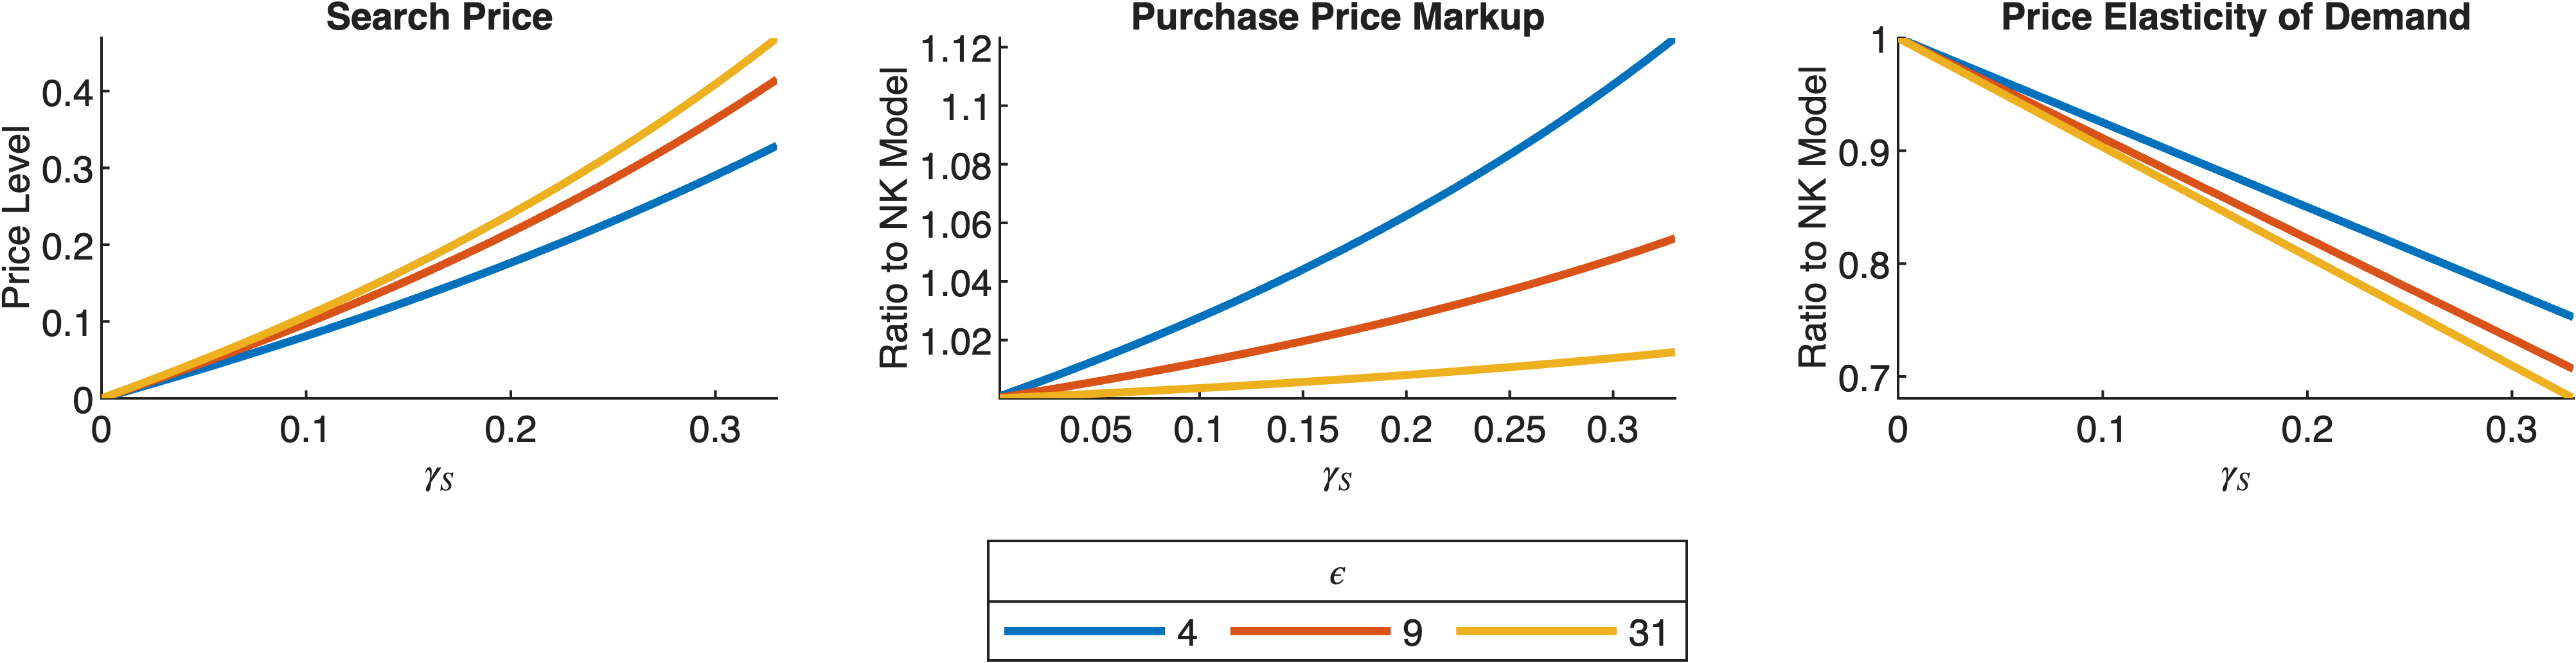
\includegraphics[width=\textwidth]{fig_1_stst_ps_mp.png}\\%
	{\tiny \singlespacing NOTE: The figure shows relative steady-state values of the NK-SaM model over the benchmark model for different calibrations. Search prices, $P_S$, are given as a real price level (consumption good as the numeraire) as they are zero in the benchmark model. Benchmark NK model and NK-SaM model are calibrated to different levels of relative home to market labor as shopping time is included in this measure for the benchmark model (see also \cref{sec:calibration}). This feature leads to a relative output steady-state not equal to one for $\gamma_S=0$.\par}%
\end{figure}%
% Description
\Cref{fig:stst_eps_gamES} shows how \eqref{stst:marg_search}, \eqref{stst:mc}, and \eqref{stst:price_elasticity} respond to different $\epsilon$ as we increase $\gamma_S$. Search prices increase in $\gamma_S$ as search effort becomes more productive in creating matches and households shift their time to search. This effect is especially prevalent if consumption goods are easily substitutable (goods markets are highly competitive) and search is highly productive. We find search prices of $39\%$ of the purchase price for the calibrated model. The \emph{price elasticity} relative to the benchmark model decreases in search price as $\gamma_S$ increases, especially for high $\epsilon$. It decreases up to $30\%$. The lower \emph{price elasticity} maps directly into higher price markups, especially if $\epsilon$ is low. Firms gain from high search effort as their capacity utilization and thus productivity increases. Having significant market power due to low $\epsilon$, firms do not pass through a significant share of those productivity gains. This pattern leads to an increase of price markups of up to $12\%$. In the calibrated model, we set $\epsilon$ by targeting markups across models which implies an identical price elasticity in steady-state across models\footnote{Baseline markup is $20\%$ across both models. See \cref{sec:calibration}.}. This approach implies a higher $\epsilon$ in the NK-SaM model, thus more competitive goods markets achieving the same level of price elasticity.\\%
% Household steady-state (KPR)
%--------------------------------------------------------------------------
The steady-state of the representative household is determined by marginal utility out of market consumption net of marginal search cost \eqref{stst:muc} given by %
\begin{align}%
	muc \; = & \; \xi_{C_M} \left( 1 - \phi_\epsilon \right) C^{-\sigma},\label{stst:muc}%
\end{align}%
where $\xi_{C_M} = \chi_{C_M}\frac{C}{C_M}$ and $\chi_{C_M}=\left(1-\gamma_H\right)\left(\frac{C_M}{C}\right)^{\Gamma_H}$ with composite consumption, $C$, given by \eqref{eq:composite_consumption} and $C_H = \left[ \frac{\gamma_H}{\mu_H} C^{1-\Gamma_H}\right]^{\frac{1}{1+\nu_H-\Gamma_H}}$. Marginal utility of market consumption \eqref{stst:muc} increases in $\xi_{CM}$ and $C^{-\sigma}$. Both elements describe the trade-off with home production. Adding goods market SaM decreases \eqref{stst:muc} in the super-elasticity, $\phi_\epsilon$, as the search price increases. Hence, \eqref{stst:muc} decreases in the \emph{price elasticity} as shown in \cref{fig:stst_eps_gamES}. However, $\xi_{C_M}$ is higher in the NK-SaM model as search effort is a separate margin described by $\phi_\epsilon$ in the NK-SaM model but part of $\xi_{C_M}$ in the benchmark model. Overall, marginal utility of market consumption is higher in the NK-SaM model with an increase of about $7\%$ for the calibrated model.\\%
% Real GDP steady-state
%--------------------------------------------------------------------------
The size of the market economy derives from \emph{steady-state real GDP} - determined by production capacity and its utilization rate - and is given by%
\begin{align}%
	Y \; = \; C_M \; = & \; q \cdot \underbrace{\left[ \frac{muc}{\mu_M} \cdot \frac{\epsilon_W-1}{\epsilon_W} \cdot q \cdot mc \right]^{\frac{1}{\nu_M}}}_{\text{Total labor allocation} \; (H_M)},\label{eq:stst_gdp}%
\end{align}%
where production capacity is determined by equilibrium labor supply, $\mathcal{Y}_M = H_M$. As in the benchmark model, equilibrium labor supply increases in $muc$ as the opportunity cost of labor supply decrease, in $\epsilon_W$ as wage markup decrease, and in $mc$ as price markups decrease. Adding goods market SaM increases labor supply as $muc$ increases (see \eqref{stst:muc}) and decreases labor demand as productivity decreases in $q$ and price markups increase in $\gamma_S$.\\%
% QUANTITATIVE SIMULATIONS ON REAL GDP
%--------------------------------------------------------------------------
Stedy-state output decreases in $\gamma_S$ which implies lower $muc$ as shown in \eqref{stst:muc} and lower $mc$ as shown in \eqref{stst:mc}. A lower elasticity of substitution, $\epsilon$, implies a smaller impact on $muc$ but a larger impact on $mc$. However, while a lower $\epsilon$ lowers steady-state output, its impact is symmetric across the benchmark and NK-SaM models\footnote{The additional results can be found in \ref{sec:stst_add_gdp}.}. A matching efficiency, $\psi$, below one additionally reduces output both through lower labor productiivty and lower utilization of given production capacity. Overall, we find a decrease in real GDP of up to $33\%$ and of $20\%$ for the calibrated model.%
% Lemma: Steady-state section summary
%--------------------------------------------------------------------------
\begin{lemma}%
	Steady-state real GDP decreases in the NK-SaM model compared to the benchmark model as available production capacity decreases due to higher \textbf{search costs} (lower labor supply and demand) and lower \textbf{labor productivity} (lower labor demand). This effect is amplified by \textbf{under-utilized} available production capacity.%
\end{lemma}%
%--------------------------------------------------------------------------
% 4. MODEL DYNAMICS
%--------------------------------------------------------------------------
%--------------------------------------------------------------------------
% The Dynamics of the Trade-Off between Prices and Capacity Utilization
%--------------------------------------------------------------------------
\section{The Dynamics of the Trade-Off between Prices and Capacity Utilization}\label{sec:dynamics}%
% INTRODUCTION
In the short-run, the model economy is driven by a trade-off between sticky purchase prices and flexible search prices. Firms maximize their profits by balancing prices and capacity utilization. This trade-off is determined by the behavior of the price elasticity (of demand), capacity utilization, and alternative time-use in home production. In this section, we derive the (intertemporal) decision rules to highlight the impact of goods market SaM over the business cyle. The model is linearized around its deterministic steady-state. Variables with a hat indicate percentage (point) deviations\footnote{Variables that are given in levels in the non-linear model are approximated by percentage deviations from steady-state and variables given in percent in the non-linear model are approximated by percentage point deviations from steady-state.} from steady-state, e.g. $\hat{x}_t$. Detailed derivations can be found in \ref{sec:full_optimization} and \ref{sec:reduced_form_app}.%
% Search and Utilization in Goods Markets
%--------------------------------------------------------------------------
\subsection{Search and Utilization in Goods Markets}%
% Search Price
%--------------------------------------------------------------------------
\paragraph{Search Prices}%
Firms target an optimal search price of households\footnote{Firms target a constrained optimal equilibrium on the goods market with fixed shares of search effort and goods supply due to the CES matching function and directed search following \cite{moenCompetitiveSearchEquilibrium1997}.} -- defined as marginal search disutility of a matched good denominated in the numeraire good -- by setting purchase prices and available goods in a trade-off between marginal costs and capacity utilization to maximize their profits. The \emph{search price} is given by%
\begin{align}\label{eq:lin_marg_search}%
	\boldsymbol{\hat{P}_{S,t}} \; = & \; \epsilon \cdot \boldsymbol{\hat{mc}_t} + \frac{\Gamma_S}{1-\phi_\epsilon}\frac{1+\phi_\gamma}{\psi\phi_\gamma}  \left( \boldsymbol{\hat{q}_t} - \boldsymbol{\hat{\psi}_t} \right) - \left(1+\phi_\gamma\right) \boldsymbol{\hat{\epsilon}_t},%
\end{align}%
with goods market tightness given by $\hat{x}_t = \hat{q}_t - \hat{\psi}_t$. The search price increases in marginal costs as the price markup decreases. If goods markets are competitive ($\epsilon$ is high), households respond to decreasing price markups by increasing their search effort (search price) more. If matching inputs are complements ($\Gamma_S<0$), excess search effort is not (as) productive. Households respond by decreasing unproductive search effort in tight goods markets to reduce search prices. An exogenous increase in $\hat{\epsilon}_t$ increases competition on the goods market which leads to higher pass-through of marginal costs to prices and thus lower variation in search prices. The \emph{price elasticity (of demand)} is given by%
\begin{align}\label{eq:lin_price_elasticity}%
	\boldsymbol{\hat{\Xi}_t} \; = & \; -\phi_\epsilon \boldsymbol{\hat{P}_{S,t}} + \boldsymbol{\hat{\epsilon}_t},%
\end{align}%
which increases in $\hat{\epsilon}_t$ as goods are greater substitutes and decreases in search prices as purchase prices comprise a smaller share of consumption costs. Demand becomes less elastic in search prices. Its slope is determined by the steady-state super-elasticity, $\phi_\epsilon$\footnote{Variation in the \emph{price elasticity} does not vanish for perfectly substitutable goods, $\epsilon \rightarrow \infty$. Its variation in $\hat{P}_{S,t}$ increases as $\phi_\epsilon$ increases in $\epsilon$.}.%
% Capacity Utilization
%--------------------------------------------------------------------------
\paragraph{Capacity Utilization}%
For any amount of available goods on a goods market, the amount of search effort supplied determines \emph{capacity utilization}. It given by%
\begin{align}\label{eq:lin_caput}%
	\boldsymbol{\hat{q}_t} \; = & \; \frac{\psi \phi_\gamma}{1+\nu_S} \left[ \left(1-\phi_\epsilon\right) \boldsymbol{\hat{P}_{S,t}} - \left(\nu_S+\phi_{C}\right) \boldsymbol{\hat{Y}_t} - \boldsymbol{\hat{\mu}_{S,t}} \right] + \left(1+\phi_\gamma\right) \boldsymbol{\hat{\psi}_t},%
\end{align}%
which exogenously increases in matching efficiency, $\hat{\psi}_t$, and decreases in the level of search disutility, $\hat{\mu}_{S,t}$. An increase in search effort implies a relatively smaller increase in search prices if the super-elasticity, $\phi_\epsilon$, is small. The implicit search effort in search prices decreases in the convexity of search disutility, $\nu_S$, which increases as output expands and in turn decreases the impact of search prices on capacity utilization. Home production and a consumption wealth effect are summarized by $\phi_C = \left(1-\Gamma_H\right)\left(1-\phi_{C_M}\right) + \sigma \phi_{C_M}$ with $\phi_{C_M} = \chi_{C_M} \left(1-\frac{1-\Gamma_H-\sigma}{1-\Gamma_H+\nu_H}\left(1-\chi_{C_M}\right)\right)^{-1}$ determining the market consumption elasticity of overall consumption. $\phi_{C_M}$ decreases as home production makes up a larger share of consumption and/or is harder to substitute, which in turn increases $\phi_C$ and thus reduces the variation of capacity utilization over the business cycle. The wealth effect, $\sigma\phi_{C_M}$, decreases the response of capacity utilization to search effort as well. However, it decreases in the level of home production. Overall, the impact of search effort on capacity utilization increases in $\phi_\gamma$ as search effort is more productive and salient.%
% Lemma capacity utilization
\begin{lemma}\label{lem:caput}%
	Variation in capacity utilization is driven by a trade-off between price markups and capacity utilization summarized by the \textbf{price elasticity channel} \eqref{eq:lin_price_elasticity} and the \textbf{capacity utilization channel} \eqref{eq:lin_caput}. High search prices imply high capacity utilization but require low price markups. Variation in capacity utilization is strictly increasing in the substitutability of matching inputs, $\Gamma_S$, as shown by \eqref{eq:lin_marg_search}.%
\end{lemma}%
% Price and Wage Setting in Light of Search Prices
%--------------------------------------------------------------------------
\subsection{Price and Wage Setting in Light of Search Prices}%
% Optimal Price-Setting
%--------------------------------------------------------------------------
\paragraph{Optimal Price-Setting}%
The \emph{centerpiece of the model} is the trade-off between flexible search prices and sticky purchase prices. It is summarized by the \emph{NK Phillips curve} given by%
\begin{align}\label{eq:lin_nkpc}%
	\boldsymbol{\hat{\pi}_t} \; = & \; \frac{1+\phi_\gamma}{\kappa_P} \left[ \epsilon\left(1-\phi_\epsilon\right) \boldsymbol{\hat{mc}_t} + \frac{\Gamma_S}{\psi} \left(\boldsymbol{\hat{q}_t}-\boldsymbol{\hat{\psi}_t}\right) - \frac{\boldsymbol{\hat{\epsilon}_t}}{\epsilon-1} \right] + \beta \mathbb{E}_t \boldsymbol{\hat{\pi}_{t+1}},%
\end{align}%
where inflation increases in marginal costs\footnote{Marginal costs determine the labor share, $\hat{ls}_t = \hat{mc}_t$, as in the benchmark model. We use this equivalence to match the slope of the labor share Phillips curve to estimates in the literature \citep{galiInflationDynamicsStructural1999,sbordonePricesUnitLabor2002}. The estimate is potentially biased by goods market tightness. However, as long as $\Gamma_S \approx 0$, the bias is quantitatively small.} -- thus in search prices as shown by \eqref{eq:lin_marg_search} -- decreases in goods market tightness if $\Gamma_S<0$, and decreases in $\hat{\epsilon}_t$ as goods markets are more competitive. Price-setting is sluggish due to price adjustment cost, $\kappa_P$, and forward-looking.\\%
% Description of NKPC Channels
As in the benchmark model, the pass-through of marginal costs to purchase prices increase in the \emph{price elasticity}. Higher competition requires stronger price adjustment as demand for a single firm would otherwise explode leading to exploding marginal costs. Adding goods market SaM decreases the price elasticity determined by its steady-state super-elasticity, $\phi_\epsilon$, as shown by \eqref{stst:price_elasticity}. In contrast, the pass-through of marginal costs to purchase prices increases in the search effort elasticity of available capacity, $\phi_\gamma$. As search effort becomes more productive, firms can increase prices more while achieving the same capacity utilization rate, thus increasing profits. The combined effect of the two goods market SaM channels on price-setting is given by $(\epsilon+\phi_\gamma)$, which implies that the \emph{capacity utilization channel} described by $\phi_\gamma$ is larger than the \emph{price elasticity channel} given $\epsilon$\footnote{As shown in \eqref{stst:mc}, $\epsilon$ increases in $\gamma_S$ when targeting a steady-state price markup. Hence, it further steepens the slope of the Phillips curve when one targets steady-state price markups instead of calibrating $\epsilon$ directly.}. The overall effect implies a steepening of the marginal costs (labor share) slope of the Phillips curve in $\gamma_S$\footnote{If we target Phillips curve slope estimates, this finding implies higher price adjustment costs, $\kappa_P$, to balance the otherwise steeper slope.}. If goods market matching inputs are greater complements, $\Gamma_S < 0$, the pass-through of marginal costs to purchase prices decreases in goods market tightness as search effort is less ''productive''.%
% Lemma NKPC
\begin{lemma}\label{lem:nkpc}%
	The firm's price-setting trade-off between price markups and capacity utilization has two components. First, the ''flexible price component'' describing price-setting to achieve the optimal time allocation between search effort, home production, and market production, given $\epsilon$ and $\gamma_S$. And second, its trade-off with price adjustment costs, as described by \eqref{eq:lin_nkpc}.%
\end{lemma}%
% Unemployment and Wage Inflation
%--------------------------------------------------------------------------
\paragraph{Unemployment and Wage Inflation}%
The labor market features the extensive margin in a tractable way following \cite{gali2011unemployment}. Unemployment is determined by sticky wage inflation. The \emph{wage Phillips curve} is given by%
\begin{align}%
	\boldsymbol{\hat{\pi}_{W,t}} \; = & \; (-1) \frac{\nu_M \left(\epsilon_W-1\right)}{\kappa_W} \phi_u \boldsymbol{\hat{u}_t} + \beta \mathbb{E}_t \boldsymbol{\hat{\pi}_{W,t+1}},\label{eq:lin_wage_phillips}%
\end{align}%
where $\epsilon_W\geq1$, $\phi_u = \left(\frac{\epsilon_W-1}{\epsilon_W}\right)^{\frac{1}{\nu_M}}$, and $\kappa_W\geq0$. Real wages are given by $\hat{w}_t = \hat{\pi}_{W,t} - \hat{\pi}_t + w_{t-1}$ with $\hat{w}_t = \hat{mc}_t+\hat{lpr}_t$. Labor productivity is given by%
\begin{align}%
	\boldsymbol{\hat{lpr}_t} = \boldsymbol{\hat{A}_t} + \psi^{-1} \boldsymbol{\hat{q}_t},%
\end{align}%
which fluctuates in capacity utilization, $\hat{q}_t$, and productivity, $\hat{A}_t$. Adding goods market SaM adds a second endogenous real wage channel besides variation in marginal costs, $\hat{mc}_t$.%
% Consumption Euler Equation (KPR)
%--------------------------------------------------------------------------
\subsection{Intertemporal Consumption Allocation and Aggregate Demand}%
% Consumption Euler Equation (KPR)
%--------------------------------------------------------------------------
\paragraph{Consumption Euler Equation}%
Intertemporal consumption allocation of the representative household is determined by the response of output growth to changes in the real interest rate. The \emph{consumption Euler equation} is given by%
\begin{align}\label{eq:euler_lin}%
	\boldsymbol{\hat{r}_t} - \mathbb{E}_t \boldsymbol{\hat{\pi}_{t+1}} \; = & \; \phi_C \mathbb{E}_t \boldsymbol{\Delta \hat{Y}_{t+1}} + \phi_\epsilon \mathbb{E}_t \boldsymbol{\Delta \hat{P}_{S,t+1}},%
\end{align}%
where $\Delta$ indicates growth rates. Adding goods market SaM features an ''inflation-like'' term given by variations in expected search price growth, $\mathbb{E}_t \Delta \hat{P}_{S,t+1}$. Expected \emph{price elasticity growth} falls in expected search price growth. Following an increase in the real interest rate, households shift consumption less to the future if expected search price growth (implicit inflation) increases. This channel is more salient as the super-elasticity, $\phi_\epsilon$, increases.%
\begin{corollary}\label{corr:corrected_inflation}%
	From \eqref{eq:euler_lin} we can derive a \emph{corrected price inflation measure} defined by%
	\begin{align}%
		\mathbb{E}_t \boldsymbol{\hat{\pi}_{T,t+1}} \; = \; \mathbb{E}_t \boldsymbol{\hat{\pi}_{t+1}} + \phi_\epsilon \mathbb{E}_t \boldsymbol{\Delta\hat{P}_{S,t+1}},%
	\end{align}%
	which takes into account observed price inflation as well as unobserved search price inflation. Applying this inflation measure to the Euler equation results in the benchmark model Euler equation with inflation corrected for search price growth.%
\end{corollary}%
% Lemma Euler equation
\begin{lemma}\label{lem:euler}%
	The growth in expected search prices is inflationary. Goods market SaM unambiguously reduces the variation of output (consumption) following a change in the real interest rate. Changes in goods market tightness affect intertemporal consumption allocation through the \textbf{price elasticity channel}, even if price inflation is constant.%
\end{lemma}%
% Real GDP
%--------------------------------------------------------------------------
\paragraph{Real GDP}%
Goods market frictions lead to idle production capacity \emph{Real GDP} is given by%
\begin{align}\label{eq:lin_mc}%
	\boldsymbol{\hat{Y}_{t}} \; = & \; \frac{1}{\nu_M+\phi_C} \Biggl[ \boldsymbol{\hat{mc}_t} - \phi_\epsilon \boldsymbol{\hat{P}_{S,t}} - \nu_M \phi_u \boldsymbol{\hat{u}_t} + \left(1+\nu_M\right) \left( \psi^{-1} \boldsymbol{\hat{q}_t} + \boldsymbol{\hat{A}_t} \right) \Biggr],%
\end{align}%
where the response to its right-hand side determinants increases in labor supply elasticity, $\nu_M^{-1}$, and in $\phi_C$ as described by \eqref{eq:lin_caput} and in line with \cite{lesterHomeProductionSticky2014}. Marginal costs \emph{(sticky prices)} and unemployment \emph{(sticky wages)} determine its endogenous variation. Technology shocks create exogenous variation. Goods market SaM adds the \emph{price elasticity} and \emph{capacity utilization channels}. Following \cite{chari2007business}, real GDP \eqref{eq:lin_mc} can be stated as%
\begin{align*}%
	\boldsymbol{\hat{Y}_{t}} \; = & \; \nu_M^{-1} \Bigl[ \left(1+\nu_M\right) \boldsymbol{\hat{\tau}_{E,t}} - \boldsymbol{\hat{\tau}_{L,t}} \Bigr]%
\end{align*}%
with its labor and efficiency wedges defined respectively by%
\begin{align}%
	\boldsymbol{\hat{\tau}_{L,t}} \; = & \; \phi_C \boldsymbol{\hat{Y}_{t}} + \nu_M \phi_u \boldsymbol{\hat{u}_t} - \boldsymbol{\hat{mc}_t} + \phi_\epsilon \boldsymbol{\hat{P}_{S,t}},\label{eq:labor_wedge}\\%
	\boldsymbol{\hat{\tau}_{E,t}} \; = & \; \psi^{-1} \boldsymbol{\hat{q}_t} + \boldsymbol{\hat{A}_t}.\label{eq:efficiency_wedge}%
\end{align}%
The \emph{price elasticity channel} affects real GDP through the (household side) labor wedge \eqref{eq:labor_wedge} and the \emph{capacity utilization channel} affects real GDP through the efficiency wedge \eqref{eq:efficiency_wedge}. As shown in \eqref{eq:lin_marg_search}, $\hat{P}_{S,t}$ increases in $\hat{mc}_t$, which implies that the \emph{price elasticity channel} counteracts the \emph{labor demand channel} working through marginal costs. For $\Gamma_S \approx 0$, the impact of marginal costs on the labor wedge is defined by $(1-\epsilon\phi_\epsilon) \lesseqqgtr 0$\footnote{The cutoff value $\epsilon\phi_\epsilon = 1$ decreases in $\epsilon$. As price markups decrease, the price elasticity channel is more likely to dominate the labor demand channel of marginal costs. A simulation exercise showing the cutoff values of $\gamma_S$ conditional on $\epsilon$ (markups) is given in \ref{sec:cutoff_gammaES}.}. If $\epsilon \phi_\epsilon > 1$, the \emph{price elasticity channel} dominates and the labor wedge increases in marginal costs. If $\epsilon \phi_\epsilon < 1$, the \emph{labor demand channel} dominates and the labor wedge decreases in marginal costs (as in the benchmark model). For $\Gamma_S < 0$, the labor wedge can be countercyclical with $\epsilon\phi_\epsilon > 1$ as the variation of search prices in marginal costs decreases. The efficiency wedge unambiguously increases in search effort which increases in marginal costs as shown in \eqref{eq:lin_caput}.%
%--------------------------------------------------------------------------
% 5. MODEL ANALYSIS
%--------------------------------------------------------------------------
%--------------------------------------------------------------------------
% Quantifying the Impact of the Goods Market SaM on the Economy
%--------------------------------------------------------------------------
\section{Quantifying the Impact of the Goods Market SaM on the Economy}\label{sec:analysis}%
% SECTION INTRODUCTION
We determine the slopes of the reduced-form output gap model where gap variables are defined as the deviation from their flexible price counterpart\footnote{The set of equations for the flexible price economy is described in \ref{sec:simple_model_flex_price}.}, i.e. $\tilde{Y}_{t} = \hat{Y}_{t} - \hat{Y}^N_{t}$. Goods market SaM creates a countercyclical price elasticity gap which is amplified by a procyclical capacity utilization gap. Compared to the benchmark model, aggregate demand is less responsive to changes in the real interest rate while firm price-setting is more flexible following feedback effects from the capacity utilization gap. Hence, shifting shopping time from home production \citep{lesterHomeProductionSticky2014} to goods market SaM has the opposite impact on aggregate demand and supply. The model shows a trade-off between matching the procyclical efficiency wedge and the countercyclical labor wedge in the data.%
% --------------------------------------------------------------------------
% Goods Market SaM Channels in the Reduced-Form Model
% --------------------------------------------------------------------------
\subsection{Goods Market SaM Channels in the Reduced-Form Model}%
% Gap Variables of the Goods Market SaM Channels
% --------------------------------------------------------------------------
Unobserved search effort paired with sticky prices drives variation in the \emph{capacity utilization gap} (efficiency wedge gap), the \emph{price elasticity gap}, and the \emph{labor wedge gap}. They are reduced-form gap variable versions of \eqref{eq:lin_price_elasticity}, \eqref{eq:lin_mc}, and \eqref{eq:labor_wedge} given by%
\begin{align}%
	\boldsymbol{\tilde{q}_t} \; = & \; \boldsymbol{\tilde{\tau}_{E,t}} \; = \; \theta_{q,Y} \boldsymbol{\tilde{Y}_{t}} + \theta_{q,u} \boldsymbol{\tilde{u}_t},\label{eq:util_gap}\\%
	\boldsymbol{\tilde{\Xi}_{t}} \; = & \; \left(-1\right) \left[ \theta_{\Xi,Y} \boldsymbol{\tilde{Y}_{t}} + \theta_{\Xi,u} \boldsymbol{\tilde{u}_t} \right],\label{eq:price_elasticity_gap}\\%
	\boldsymbol{\tilde{\tau}_{L,t}} \; = & \; \theta_{\tau_L,Y} \boldsymbol{\tilde{Y}_{t}} + \theta_{\tau_L,u} \boldsymbol{\tilde{u}_t},\label{eq:labor_wedge_gap}%
\end{align}%
where $\theta_{q,Y} = \theta_{q,q}^{-1} \left\{\epsilon\left(1-\phi_\epsilon\right)\left[\nu_M+\phi_C\right]-\left(1-\epsilon\phi_\epsilon\right)\left[\nu_S+\phi_C\right]\right\}$ and $\theta_{q,u} = \theta_{q,q}^{-1} \epsilon\left(1-\phi_\epsilon\right)\nu_M \phi_u$ with $\theta_{q,q} = \epsilon\left(1-\phi_\epsilon\right)\Bigl[1+\nu_M-\frac{\Gamma_S}{1-\phi_\epsilon}\frac{\epsilon-1}{\epsilon}\Bigr]+\frac{1-\epsilon\phi_\epsilon}{\psi\phi_\gamma}\Bigl[1+\nu_S-\left(1+\phi_\gamma\right)\Gamma_S\Bigr]$ are the slopes of \eqref{eq:util_gap}, $\theta_{\Xi,Y} = \frac{\phi_\epsilon}{1-\phi_\epsilon} \left[ \nu_S + \phi_C + \frac{1+\nu_S}{\phi_\gamma} \frac{\theta_{q,Y}}{\psi} \right]$ and $\theta_{\Xi,u} = \frac{\phi_\epsilon}{1-\phi_\epsilon} \frac{1+\nu_S}{\phi_\gamma} \frac{\theta_{q,u}}{\psi}$ are the slopes of \eqref{eq:price_elasticity_gap}, and $\theta_{\tau_L,Y} = \phi_C - \frac{1-\epsilon\phi_\epsilon}{\epsilon \phi_\epsilon} \theta_{\Xi,Y} + \frac{\Gamma_S}{1-\phi_\epsilon}\frac{1+\phi_\gamma}{\epsilon\phi_\gamma} \frac{\theta_{q,Y}}{\psi}$ and $\theta_{\tau_L,u} = \nu_M \phi_u - \frac{1-\epsilon\phi_\epsilon}{\epsilon\phi_\epsilon} \theta_{\Xi,u} + \frac{\Gamma_S}{1-\phi_\epsilon}\frac{1+\phi_\gamma}{\epsilon\phi_\gamma}\frac{\theta_{q,u}}{\psi}$ are the slopes of \eqref{eq:labor_wedge_gap}. Variation in the \emph{capacity utilization gap} is determined by search effort productivity, $\phi_\gamma$, a \emph{labor demand channel}, and a \emph{price elasticity channel} (see \eqref{eq:labor_wedge} and \eqref{eq:efficiency_wedge}). All three channels increase in marginal costs as shown by \eqref{eq:lin_marg_search}. Variation in the \emph{price elasticity gap} is determined by search disutility convexity, $\nu_S$, home production and wealth effects, $\phi_C$, and variation in capacity utilization determined by $\theta_{q,Y}$ and $\theta_{q,u}$ (see \eqref{eq:lin_price_elasticity}). Variation in the \emph{labor wedge gap} is determined by the trade-off between the labor demand and price elasticity channels as described for \eqref{eq:labor_wedge}. \Cref{fig:slopes_5eq_util} shows how goods market SaM affects the output gap elasticity of \eqref{eq:util_gap}, \eqref{eq:price_elasticity_gap}, and \eqref{eq:labor_wedge_gap}. We apply Okun's law with a coefficient derived from data of $\frac{\tilde{u}_t}{\tilde{Y}_t} = -2.23$ \citep{knotek2007useful} to summarize the output and unemployment gap coefficients in one elasticity. Figures for the individual slopes are given in \ref{sec:slopes_add_individual}.%
% FIGURE: Capacity Utilization Slopes
\begin{figure}[t]%
	\centering%
	\caption{Variation of the Slopes of the Goods Market SaM Channels}\label{fig:slopes_5eq_util}%
	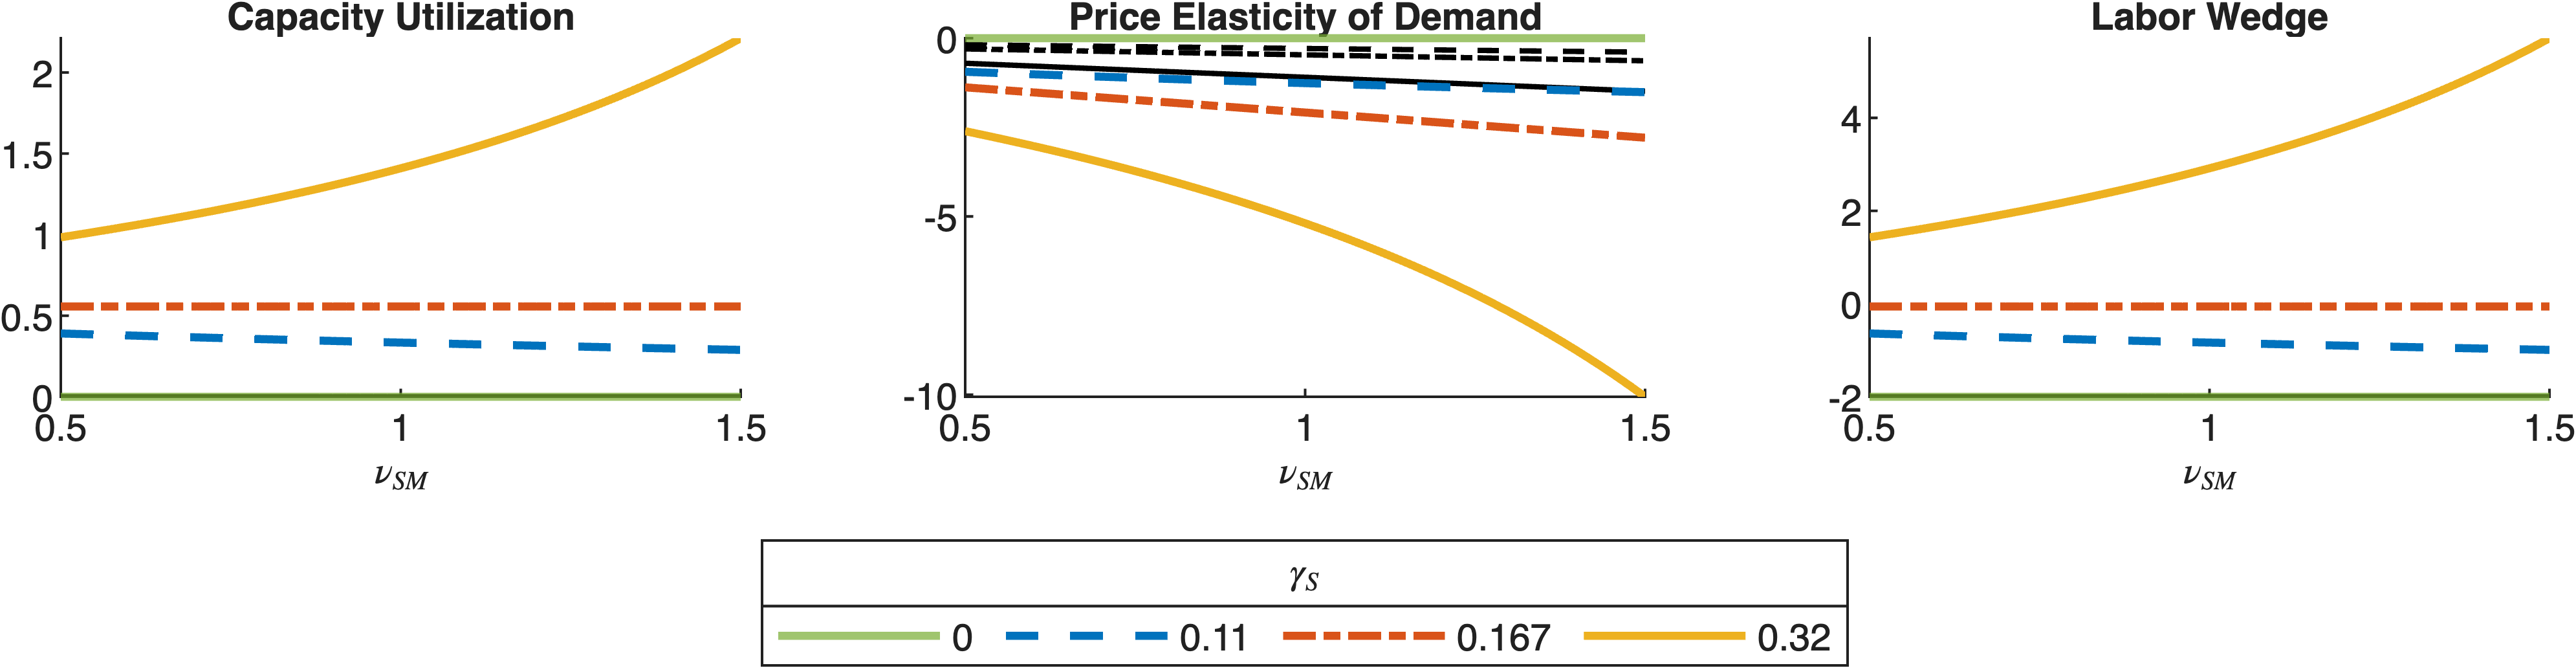
\includegraphics[width=\textwidth]{fig_2_slopes_5eq_ps_cu_okun.png}\\%
	{\tiny \singlespacing NOTE: The graphs show the impact of varying $\nu_S$ with a fixed $\nu_M$ on the slopes of the goods market SaM channels (including home production). The benchmark model is shown by the full horizontal line ($\gamma_S=0$). The NK-SaM model is shown in two variants for three different values of $\gamma_S$ indicated by the dashed, dashed-dotted, and full lines. First, the bold-colored lines show $\Gamma_S \approx 0$. Second, the thin-black lines show $\Gamma_S=-\infty$ implying an substitution elasticity of $\approx 0$ for the matching inputs indicating a Leontief matching function.\par}%
\end{figure}%
% Capacity Utilization Gap
% --------------------------------------------------------------------------
\paragraph{Capacity Utilization Gap}%
The output gap elasticity decreases as matching inputs become greater complements, $\Gamma_S \rightarrow - \infty$, and converges to zero in the limit (Leontief matching function). Variation in the capacity utilization gap depends crucially on the substitutability of search effort and goods supply. As $\gamma_S$ increases, search effort is more productive and search prices increase which decreases the steady-state price elasticity, $\epsilon(1-\phi_\epsilon)$, but increases search effort productivity, $\phi_\gamma$. The second effect dominates as the output gap elasticity of capacity utilization increases in $\gamma_S$. The impact of the relative time supply elasticity, $\nicefrac{\nu_S}{\nu_M}$, on the output gap elasticity depends on whether the \emph{labor demand} or \emph{price elasticity channel} dominate the labor wedge (see \eqref{eq:labor_wedge}). Search price variation increases in $\nu_S$ (see \eqref{eq:lin_caput}) which increases marginal costs variation (see \eqref{eq:lin_marg_search}). If the \emph{labor demand channel} dominates ($(1-\epsilon\phi_\epsilon)>0$), it follows that higher variation in marginal costs lead to a larger labor demand response and thus a smaller capacity utilization response. If the \emph{price elasticity channel} dominates ($(1-\epsilon\phi_\epsilon)<0$), the capacity utilization response is larger as the countercyclical variation in the price elasticity is larger. For $(1-\epsilon\phi_\epsilon)=0$, capacity utilization gap variation does not depend on $\nu_S$ as the two channels cancel each other out. Applying Okun's law to the calibrated model, we find an overall output gap elasticity of the capacity utilization gap of $1.41$\footnote{The elasticities of the capacity utilization gap are larger than the actual capacity utilization variation relative to real GDP. It follows from the flexible price capacity utilization being countercyclical due to home production, wealth effects and convex search disutility while sticky price capacity utilization shows a procyclical pattern. The individual elasticities of the capacity utilizaiton gap are given in \ref{sec:slopes_add_individual}. For the calibrated model, they are $1.88$ for the output gap and $1.06$ for the unemployment gap.}. The capacity utilization gap is procyclical. It implies a procyclical search effort gap determined by $\tilde{H}_{S,t} = \tilde{Y}_t + \frac{1-\gamma_S}{\gamma_S} \tilde{q}_t$ which implies an output gap elasticity of search effort of $3.87$ for the calibrated model\footnote{The slope is larger than actual search effort variation relative to real GDP variation as capacity utilization in the flexible price model is countercyclical amplifying its output gap elasticity.}.%
% Price elasticity gap
% --------------------------------------------------------------------------
\paragraph{Price Elasticity Gap}%
For $\Gamma_S = -\infty$, variation in the price elasticity gap is low and countercyclical as it decreases in the search price. For $\Gamma_S \approx 0$, the countercyclical price elasticity gap \eqref{eq:price_elasticity_gap} is amplified by variation in the capacity utilization gap \eqref{eq:util_gap}, especially if the \emph{price elasticity channel} dominates the \emph{labor demand channel}, as search prices vary more with variable search effort success rates. $\nicefrac{\nu_S}{\nu_M}$ works through the \emph{capacity utilization channel}. Applying Okun's law to the calibrated model, we find an overall output gap elasticity of the price elasticity gap of $-5.19$\footnote{The individual elasticities of the price elasticity gap are given in \ref{sec:slopes_add_individual}. For the calibrated model, they are $-6.57$ for the output gap and $-3.07$ for the unemployment gap.}. For $\Gamma_S \rightarrow -\infty$, it reduces to $-1.26$ as capacity utilization is constant. Hence, the price elasticity gap is strongly countercyclical as it is amplified by variation in the capacity utilization gap.%
% Labor wedge gap
% --------------------------------------------------------------------------
\paragraph{Labor Wedge Gap}%
For $\Gamma_S \approx 0$, the labor wedge gap is countercyclical as in the data \citep{karabarbounis2014labor} if the \emph{labor demand channel} of marginal costs dominates ($(1-\epsilon\phi_\epsilon)>0$). If the \emph{price elasticity channel} dominates ($(1-\epsilon\phi_\epsilon)<0$), the labor wedge gap is procyclical. As matching inputs become perfect complements, $\Gamma_S \rightarrow -\infty$, the output gap elasticity of the labor wedge gap is countercyclical for any $\epsilon\phi_\epsilon$ as it converges to the benchmark model. Hence, there is a trade-off between matching a procyclical efficiency wedge and a counteryclical labor wedge in the NK-SaM model. Applying Okun's law to the calibrated model, we find an overall output gap elasticity of the labor wedge gap of $2.92$\footnote{The individual elasticities of the labor wedge gap are given in \ref{sec:slopes_add_individual}. For the calibrated model, they are $4.57$ for the output gap and $3.68$ for the unemployment gap.}. The labor wedge gap is procyclical and driven by the \emph{capacity utilization channel}.% 
% --------------------------------------------------------------------------
% The Reduced-Form Five-Equation Model
% --------------------------------------------------------------------------
\subsection{The Reduced-Form Five-Equation Model}\label{sec:reduced_form_model}%
The model presented in \cref{sec:dynamics} can be summarized by a consumption Euler equation \eqref{eq:dynamicIS}, a NK price Phillips curve \eqref{eq:PRICEphillipsGAP}, a NK wage Phillips curve \eqref{eq:WAGEphillipsGAP}, a real wage growth equation \eqref{eq:realWAGEgap}, and a \cite{taylorDiscretionPolicyRules1993}-type rule \eqref{eq:taylor_lin}. The reduced-form gap model is given by%
\begin{align}%
	\boldsymbol{\hat{r}_t} - \boldsymbol{\hat{r}}^N_t - \mathbb{E}_t \boldsymbol{\hat{\pi}_{t+1}} \; = & \; \Theta_{\mathbb{M},Y} \mathbb{E}_t \boldsymbol{\Delta \tilde{Y}_{t+1}} + \Theta_{\mathbb{M},u} \mathbb{E}_t \boldsymbol{\Delta \tilde{u}_{t+1}},\label{eq:dynamicIS}\\%
	\boldsymbol{\hat{\pi}_t} \; = & \; \Theta_{\pi,Y} \boldsymbol{\tilde{Y}_{t}} + \Theta_{\pi,u} \boldsymbol{\tilde{u}_{t}} + \beta \mathbb{E}_t \boldsymbol{\hat{\pi}_{t+1}},\label{eq:PRICEphillipsGAP}\\%
	\boldsymbol{\hat{\pi}_{W,t}} \; = & \; \left(-1\right) \frac{\epsilon_W-1}{\kappa_W} \phi_u \boldsymbol{\tilde{u}_t} + \beta \mathbb{E}_t \boldsymbol{\hat{\pi}_{W,t+1}},\label{eq:WAGEphillipsGAP}\\%
	\boldsymbol{\hat{\pi}_{W,t}} - \boldsymbol{\hat{\pi}_t} \; = & \; \Theta_{w,Y} \boldsymbol{\Delta \tilde{Y}_{t}} + \Theta_{w,u} \boldsymbol{\Delta \tilde{u}_{t}},\label{eq:realWAGEgap}\\%
	\boldsymbol{\hat{r}_t} \; = & \; i_r \boldsymbol{\hat{r}_{t-1}} + \left(1-i_r\right) \Bigl[ i_\pi \boldsymbol{\hat{\pi}_t} + i_{Gap} \boldsymbol{\tilde{Y}_{t}} \Bigr] + \boldsymbol{\hat{M}_{t}},\label{eq:taylor_lin}%
\end{align}%
with the slopes for \eqref{eq:dynamicIS} given by $\Theta_{\mathbb{M},Y} = \phi_C + \theta_{\Xi,Y}$ and $\Theta_{\mathbb{M},u} = \theta_{\Xi,u}$; the slopes for \eqref{eq:PRICEphillipsGAP} given by $\Theta_{\pi,Y} = \frac{1+\phi_\gamma}{\kappa_P} \left[ \frac{1-\phi_\epsilon}{\phi_\epsilon} \theta_{\Xi,Y} - \frac{\Gamma_S}{\phi_\gamma} \frac{\theta_{q,Y}}{\psi} \right]$ and $\Theta_{\pi,u} = \frac{1+\phi_\gamma}{\kappa_P} \left[ \frac{1-\phi_\epsilon}{\phi_\epsilon} \theta_{\Xi,u} - \frac{\Gamma_S}{\phi_\gamma} \frac{\theta_{q,u}}{\psi} \right]$; and the slopes for \eqref{eq:realWAGEgap} given by $\Theta_{w,Y} = \frac{\theta_{\Xi,Y}}{\epsilon\phi_\epsilon}+\left(1-\frac{\Gamma_S}{\epsilon\left(1-\phi_\epsilon\right)}\frac{1+\phi_\gamma}{\phi_\gamma}\right)\frac{\theta_{q,Y}}{\psi}$ and $\Theta_{w,u} = \frac{\theta_{\Xi,u}}{\epsilon\phi_\epsilon}+\left(1-\frac{\Gamma_S}{\epsilon\left(1-\phi_\epsilon\right)}\frac{1+\phi_\gamma}{\phi_\gamma}\right)\frac{\theta_{q,u}}{\psi}$. It has the identical functional form as the benchmark model \citep{ercegOptimalMonetaryPolicy2000,gali2011unemployment}, thus nests the benchmark model by \Cref{prop:nosam}. The wage Phillips curve and the Taylor rule are unaffected by goods market SaM. \Cref{fig:slopes_5eq} shows how goods market SaM affects the slopes of the Euler equation \eqref{eq:dynamicIS}, the NK price Phillips curve \eqref{eq:PRICEphillipsGAP}, and the real wage growth equation \eqref{eq:realWAGEgap} compared to the benchmark model as defined in \cref{prop:nosam}.%
% Nested Model
\begin{prop}\label{prop:nosam}%
	The NK-SaM model reduces to a benchmark NK model if $\gamma_S=0$, $\mu_S=0$, and $\psi=1$. It nests the benchmark NK model as in \cite{ercegOptimalMonetaryPolicy2000}.%
\end{prop}%
\begin{proof}%
	See \ref{proof:no_sam}.%
\end{proof}%
% FIGURE: Reduced-form model slopes
\begin{figure}[t]%
	\centering%
	\caption{Variation of the Slopes of the 5-Equation Model Dynamic Equations}\label{fig:slopes_5eq}%
	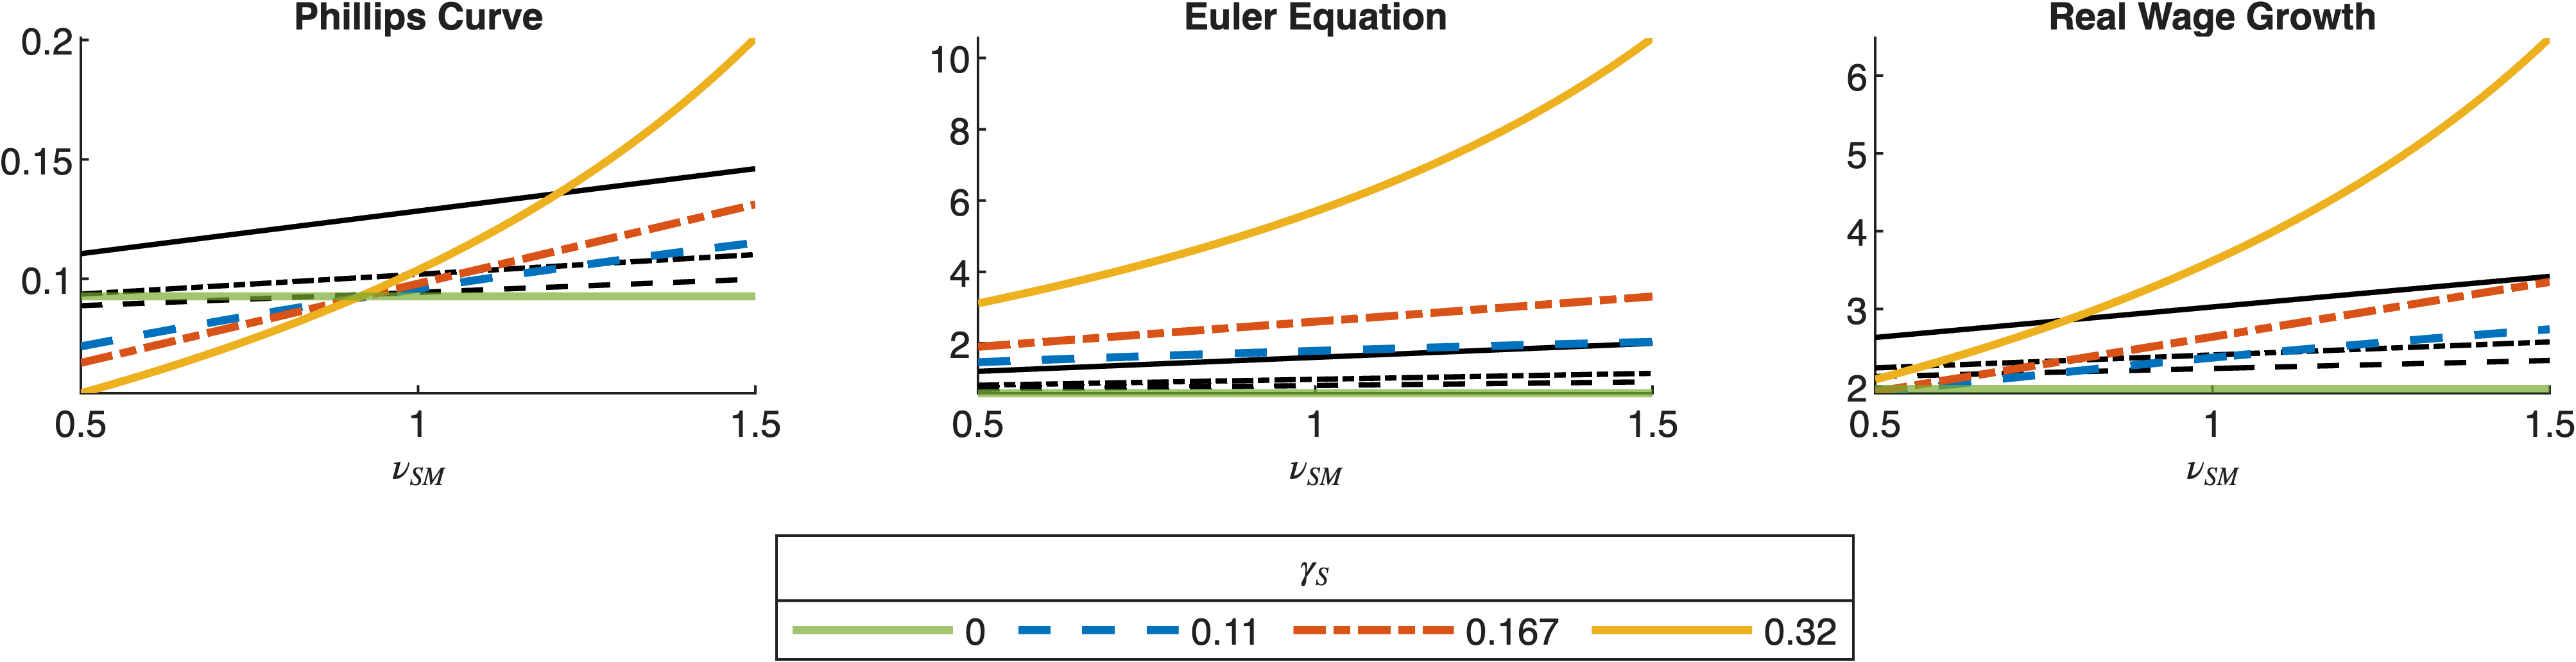
\includegraphics[width=\textwidth]{fig_3_slopes_5eq_asad_okun.png}\\%
	{\tiny \singlespacing NOTE: The graphs show the impact of varying $\nu_S$ with a fixed $\nu_M$ on the slopes of the reduced-form NK-SaM model (including home production). The benchmark model is shown by the full horizontal line ($\gamma_S=0$). The NK-SaM model is shown in two variants for three different values of $\gamma_S$ indicated by the dashed, dashed-dotted, and full lines. First, the bold-colored lines show $\Gamma_S\approx 0$. Second, the thin-black lines show $\Gamma_S=-\infty$ implying an substitution elasticity of $\approx 0$ for the matching inputs indicating a Leontief matching function.\par}%
\end{figure}%
% Euler Equation: Search Costs and Inflation
%--------------------------------------------------------------------------
\paragraph{The Consumption Euler Equation}%
% BENCHMARK AND KPR CHANNEL -> PRICE ELASTICITY
Applying Okun's law to the calibrated benchmark model, we find an overall output gap elasticity of the consumption Euler equation of $0.6$\footnote{The individual elasticities of the consumption Euler equation are given in \ref{sec:slopes_add_individual}. For the calibrated benchmark model, they are $0.6$ for the output gap and $0$ for the unemployment gap.}. A $1\%$ increase in the real interest rate gap leads to a $1.67\%$ decrease in output gap growth. Adding goods market SaM increases the overall output gap elasticity through the \emph{price elasticity channel} to $5.70$\footnote{The individual elasticities of the consumption Euler equation are given in \ref{sec:slopes_add_individual}. For the calibrated NK-SaM model, they are $7.07$ for the output gap and $3.07$ for the unemployment gap.}. A $1\%$ increase in the real interest rate gap leads to a $0.18\%$ decrease in output gap growth -- a response approximately ten times smaller compared to the benchmark model. This result brings the consumption Euler equation slope significantly closer to the empirical literature \citep{ascari2021empirical} which estimates a slope close to zero.\\%
% ROBUSTNESS AND OVERALL
The results are qualitatively robust but vary quantitatively with the calibration of goods market SaM parameters between $0.71$ and $10.57$ (see \cref{fig:slopes_5eq}). Following the discussion for \eqref{eq:price_elasticity_gap}, the overall output gap elasticity increases especially in $\nu_S$ as $\Gamma_S \approx 0$ and $\gamma_S$ is large -- thus, when the variation in the \emph{price elasticity gap} is high. Adding goods market SaM implies that monetary policy must adjust its interest rates (significantly) more to achieve the same impact on output as in benchmark model. A countercyclical \emph{price elasticity gap} reduces the impact of real interest rate gap changes. The size of the impact depends on the \emph{capacity utilization gap} as shown in \eqref{eq:util_gap}. For $\Gamma_S \rightarrow - \infty$, the overall output gap elasticity is close to the benchmark model with $1.60$.%
% LEMMA EULER EQUATION
\begin{lemma}%
	The inverse of the output gap elasticity of the consumption Euler equation decreases in $\nicefrac{\nu_S}{\nu_M}$, $\gamma_S$, and $\Gamma_S$. The countercyclical pattern of the \textbf{price elasticity} increases in all three parameters, making the search price a more salient feature of overall consumption costs. It follows that monetary policy has a smaller impact on aggregate demand as goods market prices comprise a smaller share of the overall consumption costs.%
\end{lemma}%
% Phillips Curve: Tradeoff between Search Effort and Sticky Prices
%--------------------------------------------------------------------------
\paragraph{The Price Phillips Curve}%
% BENCHMARK AND KPR CHANNELS
Applying Okun's law to the calibrated benchmark model, we find an overall output gap elasticity of the price Phillips curve of $0.093$\footnote{The individual elasticities of the price Phillips curve are given in \ref{sec:slopes_add_individual}. For the calibrated benchmark model, they are $0.133$ for the output gap and $0.090$ for the unemployment gap.}, with a price adjustment costs parameter\footnote{We recalibrate the price adjustment costs parameter, $\kappa_P$, for each parameter specification to match the labor share Phillips curve slope in the data (see \ref{sec:add_calibration_strategy}). For the NK-SaM model, it is constant across all specifications if $\Gamma_S=0$ and changes only very slightly across different calibrations for $\Gamma_S \neq 0$.} $\kappa_P$ of $128$. A $1\%$ increase of the output gap leads to $0.088\%$-point increase of the inflation rate. Adding goods market SaM increases the overall output gap elasticity to $0.104$\footnote{The individual elasticities of the price Phillips curve are given in \ref{sec:slopes_add_individual}. For the calibrated NK-SaM model, they are $0.131$ for the output gap and $0.061$ for the unemployment gap.} -- a response approximately $12\%$ larger compared to the benchmark model -- although the price adjustment costs parameter $\kappa_P$ increases to $188$. The countercyclical \emph{price elasticity gap} leads to a larger pass-through of marginal costs to prices in the NK-SaM model.\\%
% ROBUSTNESS
As shown in \cref{fig:slopes_5eq}, the overall output gap slope of the NK-SaM model varies between $0.052$ and $0.201$ for different goods market SaM calibrations. It depends on $\nicefrac{\nu_S}{\nu_M}$ whether price-setting is more or less flexible than in the benchmark model. If $\nicefrac{\nu_S}{\nu_M}$ is low, firms adjust prices less than in the benchmark model. As search effort disutility is less convex than labor supply disutility, firms prefer to adjust supply through the capacity utilization margin rather than the price margin, vice-versa. This trade-off only matters if matching inputs are substitutes and it is more pronounced as search effort productivity increases in $\gamma_S$.\\%
% AGGREGATE EFFECTS & SUPER-ELASTICITY
Adding goods market SaM adds goods market tightness (capacity utilization) as a third dimension to a firm's price-setting decision. Firms adjust more along the margin with the less convex cost function curvature. The impact depends on the variation of the \emph{price elasticity channel} as shown in \eqref{eq:price_elasticity_gap}. For the calibrated model, inflation varies more in response to variation in the output gap compared to the benchmark model. As the relationship  between inflation and the labor share is fixed to its empirical value, it follows that the output gap varies less compared to inflation in the NK-SaM model.%
% LEMMA PHILLIPS CURVE
\begin{lemma}%
	Each firm sets prices to target an optimal share of matching inputs given the CES matching function. The slope of the output gap price Phillips curve increases in $\nicefrac{\nu_S}{\nu_M}$, as firms adjust prices more aggressively to dampen changes in search effort. The variation in prices increases for high $\gamma_S$ and $\Gamma_S$ as search effort is a more productive matching input and thus justifies larger price changes (thus higher price adjustment costs).%
\end{lemma}%
% Real Wage Growth
%--------------------------------------------------------------------------
\paragraph{Real Wage Growth}%
% BENCHMARK KPR 
Applying Okun's law to the calibrated benchmark model, we find an overall output gap elasticity of real wage growth of $1.97$\footnote{The individual elasticities of real wage growth are given in \ref{sec:slopes_add_individual}. For the calibrated benchmark model, they are $2.83$ for the output gap and $1.92$ for the unemployment gap.}. Adding goods market SaM increases it to $3.62$\footnote{The individual elasticities of real wage growth are given in \ref{sec:slopes_add_individual}. For the calibrated NK-SaM model, they are $4.67$ for the output gap and $2.36$ for the unemployment gap.} -- a response approximately $84\%$ larger than in the benchmark model. A countercyclical \emph{price elasticity gap} leads to larger variation in the marginal rate of substitution and a procyclical \emph{capacity utilization gap} leads to larger variation in labor productivity. Both increase the responsiveness of real wage growth to output gap growth. The results depend on the calibration of the goods market SaM parameters. The discussion of $\nicefrac{\nu_S}{\nu_M}$ as for \eqref{eq:PRICEphillipsGAP} applies as inflation affects real wage growth directly. As shown in \cref{fig:slopes_5eq}, the overall output gap slope of the NK-SaM model varies between $1.92$ and $6.49$. Hence, for the majority of calibrations, real wage growth is more responsive to output gap growth compared to the benchmark model, especially if $\nu_S$ is high, $\Gamma_S \approx 0$, and $\gamma_S$ is high.%
% Aggregate Impact
%--------------------------------------------------------------------------
\paragraph{Aggregate Impact}%
The overall impact of goods market SaM on the model economy depends on the interaction of the price Phillips curve, the consumption Euler equation, and real wage growth. The slopes of the Euler equation and real wage growth increase with goods market SaM in the analyzed parameter range, while the price Phillips curve shows ambiguous changes depending on $\nicefrac{\nu_S}{\nu_M}$. Price inflation can be either less or more responsive to the business cycle. We assume two cases: First, search effort supply is sufficiently more elastic than labor supply, i.e. $\nicefrac{\nu_S}{\nu_M} = 0.5$. And second, search effort supply is sufficiently less elastic than labor supply, i.e. $\nicefrac{\nu_S}{\nu_M} = 1.5$. As shown in \cref{fig:slopes_5eq}, $\bar{\nu}_{SM}$ describes the intersection of the the benchmark and NK-SaM Phillips curve slopes. The aggregate impact of the two cases is laid out in \cref{cor:agg_impact_sticky_price}. Quantitative simulations are provided in \cref{sec:simulations}.%
% COROLLARY CASE DISTINCTION
\begin{corollary}\label{cor:agg_impact_sticky_price}%
	Case 1: For $\frac{\nu_S}{\nu_M} < \bar{\nu}_{SM}$, a flatter Phillips curve amplifies nominal effects while a flatter Euler equation dampens them. The two effects counteract each other.\\%
	Case 2: For $\frac{\nu_S}{\nu_M} > \bar{\nu}_{SM}$, a steeper Phillips curve and a flatter Euler equation dampen nominal effects. The two effects amplify each other.%
\end{corollary}%
%--------------------------------------------------------------------------
% 6. SIMULATIONS
%--------------------------------------------------------------------------
%--------------------------------------------------------------------------
% XX. Simulation Analysis
%--------------------------------------------------------------------------
\section{Simulation Analysis}\label{sec:simulations}%
% Introduction
In this section, we analyze the aggregate impact of goods market SaM on the model economy for business cycle shocks using impulse response (IRF) analysis. To highlight the impact of the \emph{capacity utilization} and \emph{price elasticity channels}, we construct different scenarios for the NK-SaM model with (1) perfect matching complements\footnote{This scenario studies the idea of search effort as a cyclical component creating disutility to the household and a trade-off in time allocation, however, not affecting capacity utilization. As there is no clear evidence on the search effort elasticity of matching, this scenario acts as a lower bound of the impact of goods market SaM on the NK model.}, (2) a Cobb-Douglas matching function, and (3) a CES matching functions with weak complements, $\Gamma_S = -2.7$. These three scenarios are given by the blue, red, and yellow curves respectively in \cref{fig:irf_default_tfp,fig:irf_default_policy,fig:irf_default_search_effort}. We compare the NK-SaM model to our benchmark model which is shown by the grey areas in the same figures. We use Dynare \citep{adjemian2024dynare} to solve and simulate the model economy.%
%SHORT OVERVIEW OF RESULTS%
%--------------------------------------------------------------------------
% Supply and Demand Shocks in the NK-SaM Model
%--------------------------------------------------------------------------
\subsection{Supply and Demand Shocks in the NK-SaM Model}%
% Technology Shocks
%--------------------------------------------------------------------------
\paragraph{Technology Shocks}%
% TEXTBOOK DESCRIPTION & PERFECT COMPLEMENTS
\Cref{fig:irf_default_tfp} shows IRFs to an expansionary technology shock. The benchmark model IRFs to an expansionary technology shock show a significant and persistent increase in real GDP. Real wages increase as productivity increases exogenously. Prices decrease slowly due to sticky prices, leading to a countercyclical output gap and a procyclical labor wedge. Capacity utilization, search effort, and the price elasticity are constant. Adding goods market SaM with perfect matching input complements shows the same qualitative behavior of the IRFs. However, the second cost of consumption increasing in search effort reduces the IRF of real GDP compared to the benchmark model. The price elasticity decreases in search prices (search effort) leading to lower competition on the goods market, lower aggregate demand, higher markups, and a larger labor wedge (lower real wages and higher unemployment). Firms respond by cutting prices further to attract additional demand. However, overall production increases less compared to the benchmark model.\\%
% FIGURE: IRFs to a Technology Shock
\begin{figure}[t]%
	\centering%
	\caption{Channel Comparison - IRFs to an Expansionary Technology Shock}\label{fig:irf_default_tfp}%
	\vspace{-0.1in}%
	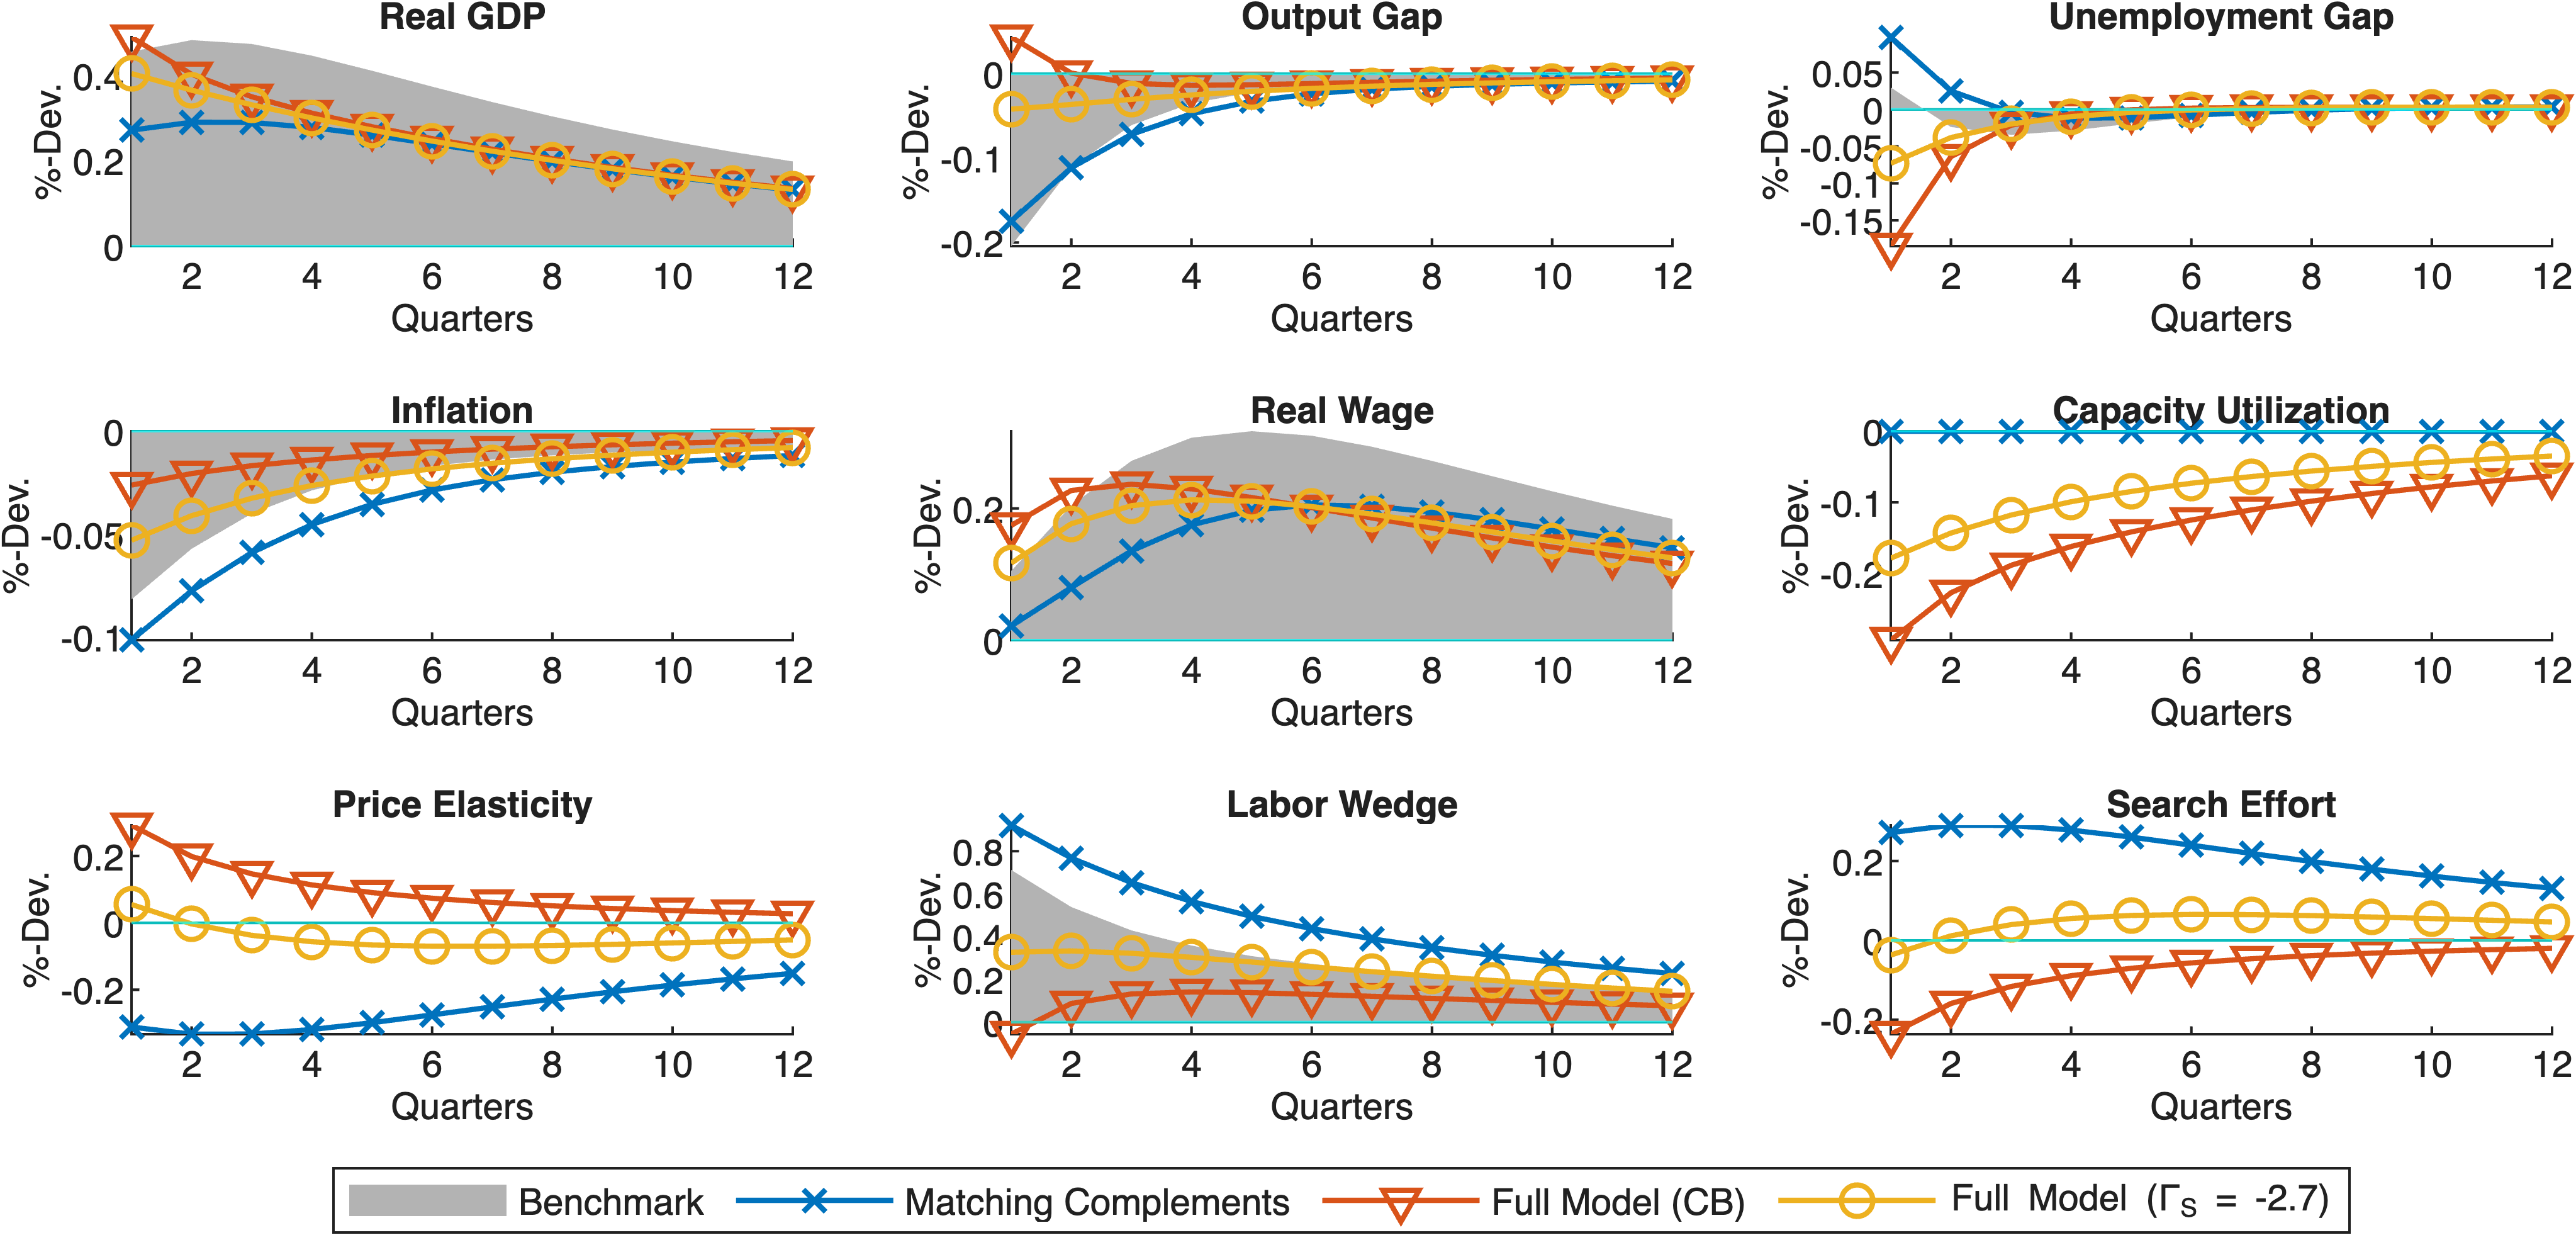
\includegraphics[width=\textwidth]{fig_4_irf_default_tfp.png}%
	\vspace{-0.1in}%
	{\tiny \singlespacing NOTE: The figure shows IRFs to a one standard deviation expansionary technology shock using the model presented in \cref{sec:model} and \cref{sec:dynamics}. The benchmark model follows \cref{prop:nosam}, the ''matching complements'' model sets $\Gamma_S = -\infty$, the CES model sets $\Gamma_S = -2.7$, the Cobb-Douglas model is calibrated as in \cref{tab:calibration}.\par}%
\end{figure}%
% CB GOODS MARKET SAM
For $\Gamma_S = 0$, real GDP initially shows a larger response compared to the benchmark model leading to a brief positive deviation of the output gap. A significant drop in capacity utilization -- in line with \cite{basuAreTechnologyImprovements2006,huo2023utilization} -- decreases search prices (search effort) and increases the price elasticity which raises competition on the goods market. Hence, aggregate demand and output increase despite firms only slightly cutting prices. This effect is strong enough to create a countercyclical unemployment response contrary to the NK literature \citep{francis2005technology,gali1999technology} but in line with \cite{safonova2017home,faccini2022importance}. Real wages increase initially more than in the benchmark model due to strong labor demand. However, as capacity utilization (labor productivity) is low, real wage expansion is overall lower compared to the benchmark model. Firms do not cut their prices further to attract additional demand as search effort is less effective as demand expands.\\%
% OVERALL TECHNOLOGY SHOCK & CES FUNCTION
Overall, introducing goods market SaM with a Cobb-Douglas matching function makes the NK-SaM model in response to a technology shock look more like a RBC model as output gap and inflation deviations are small while real GDP and employment are strongly procyclical. This pattern follows from higher competition on the goods market induced by a procyclical price elasticity amplified by variation in capacity utilization. Second moments of the simulation in \cref{tab:simul_stats} confirm those findings. For $\Gamma_S = -2.7$, the IRFs converge back to the benchmark model but the qualitative impact on the IRFs is largely in line with $\Gamma_S = 0$ except for the price elasticity which becomes slightly countercyclical.%
% Demand Shocks
%--------------------------------------------------------------------------
\paragraph{Demand Shocks}%
% GENERAL DESCRIPTION & TEXTBOOK DESCRIPTION & PERFECT COMPLEMENTS
\Cref{fig:irf_default_policy} shows IRFs to an expansionary monetary policy shock\footnote{The IRFs to a discount rate shock are identical to the IRFs of the moentary policy shock. The two shocks comprise the demand shocks in this economy.}. The IRFs of the benchmark model show a significant and persistent increase in real GDP. Households increase consumption as the central bank cuts its nominal interest rate. As prices are sticky, price markups and the labor wedge decrease and real wages increase inducing an output expansion. Capacity utilization, search effort, and the price elasticity are constant. Adding goods market SaM with perfect matching input complements shows the same qualitative behavior as the benchmark model. The price elasticity decreases in search prices (search effort) which reduces competition on the goods market and thus the real GDP response by half compared to the benchmark model and in line with \cref{sec:reduced_form_model}. Lower aggregate demand leads to lower production thus higher unemployment in line with lower real wages and a countercyclical labor wedge. Purchase prices increase by a similar magnitude as in the benchmark model due to the lower price elasticity and despite the drop in aggregate demand.\\%
% FIGURE: IRFs to a MONETARY POLICY SHOCK
\begin{figure}[t]%
	\centering%
	\caption{Channel Comparison - IRFs to an Expansionary Monetary Policy Shock}\label{fig:irf_default_policy}%
	\vspace{-0.1in}%
	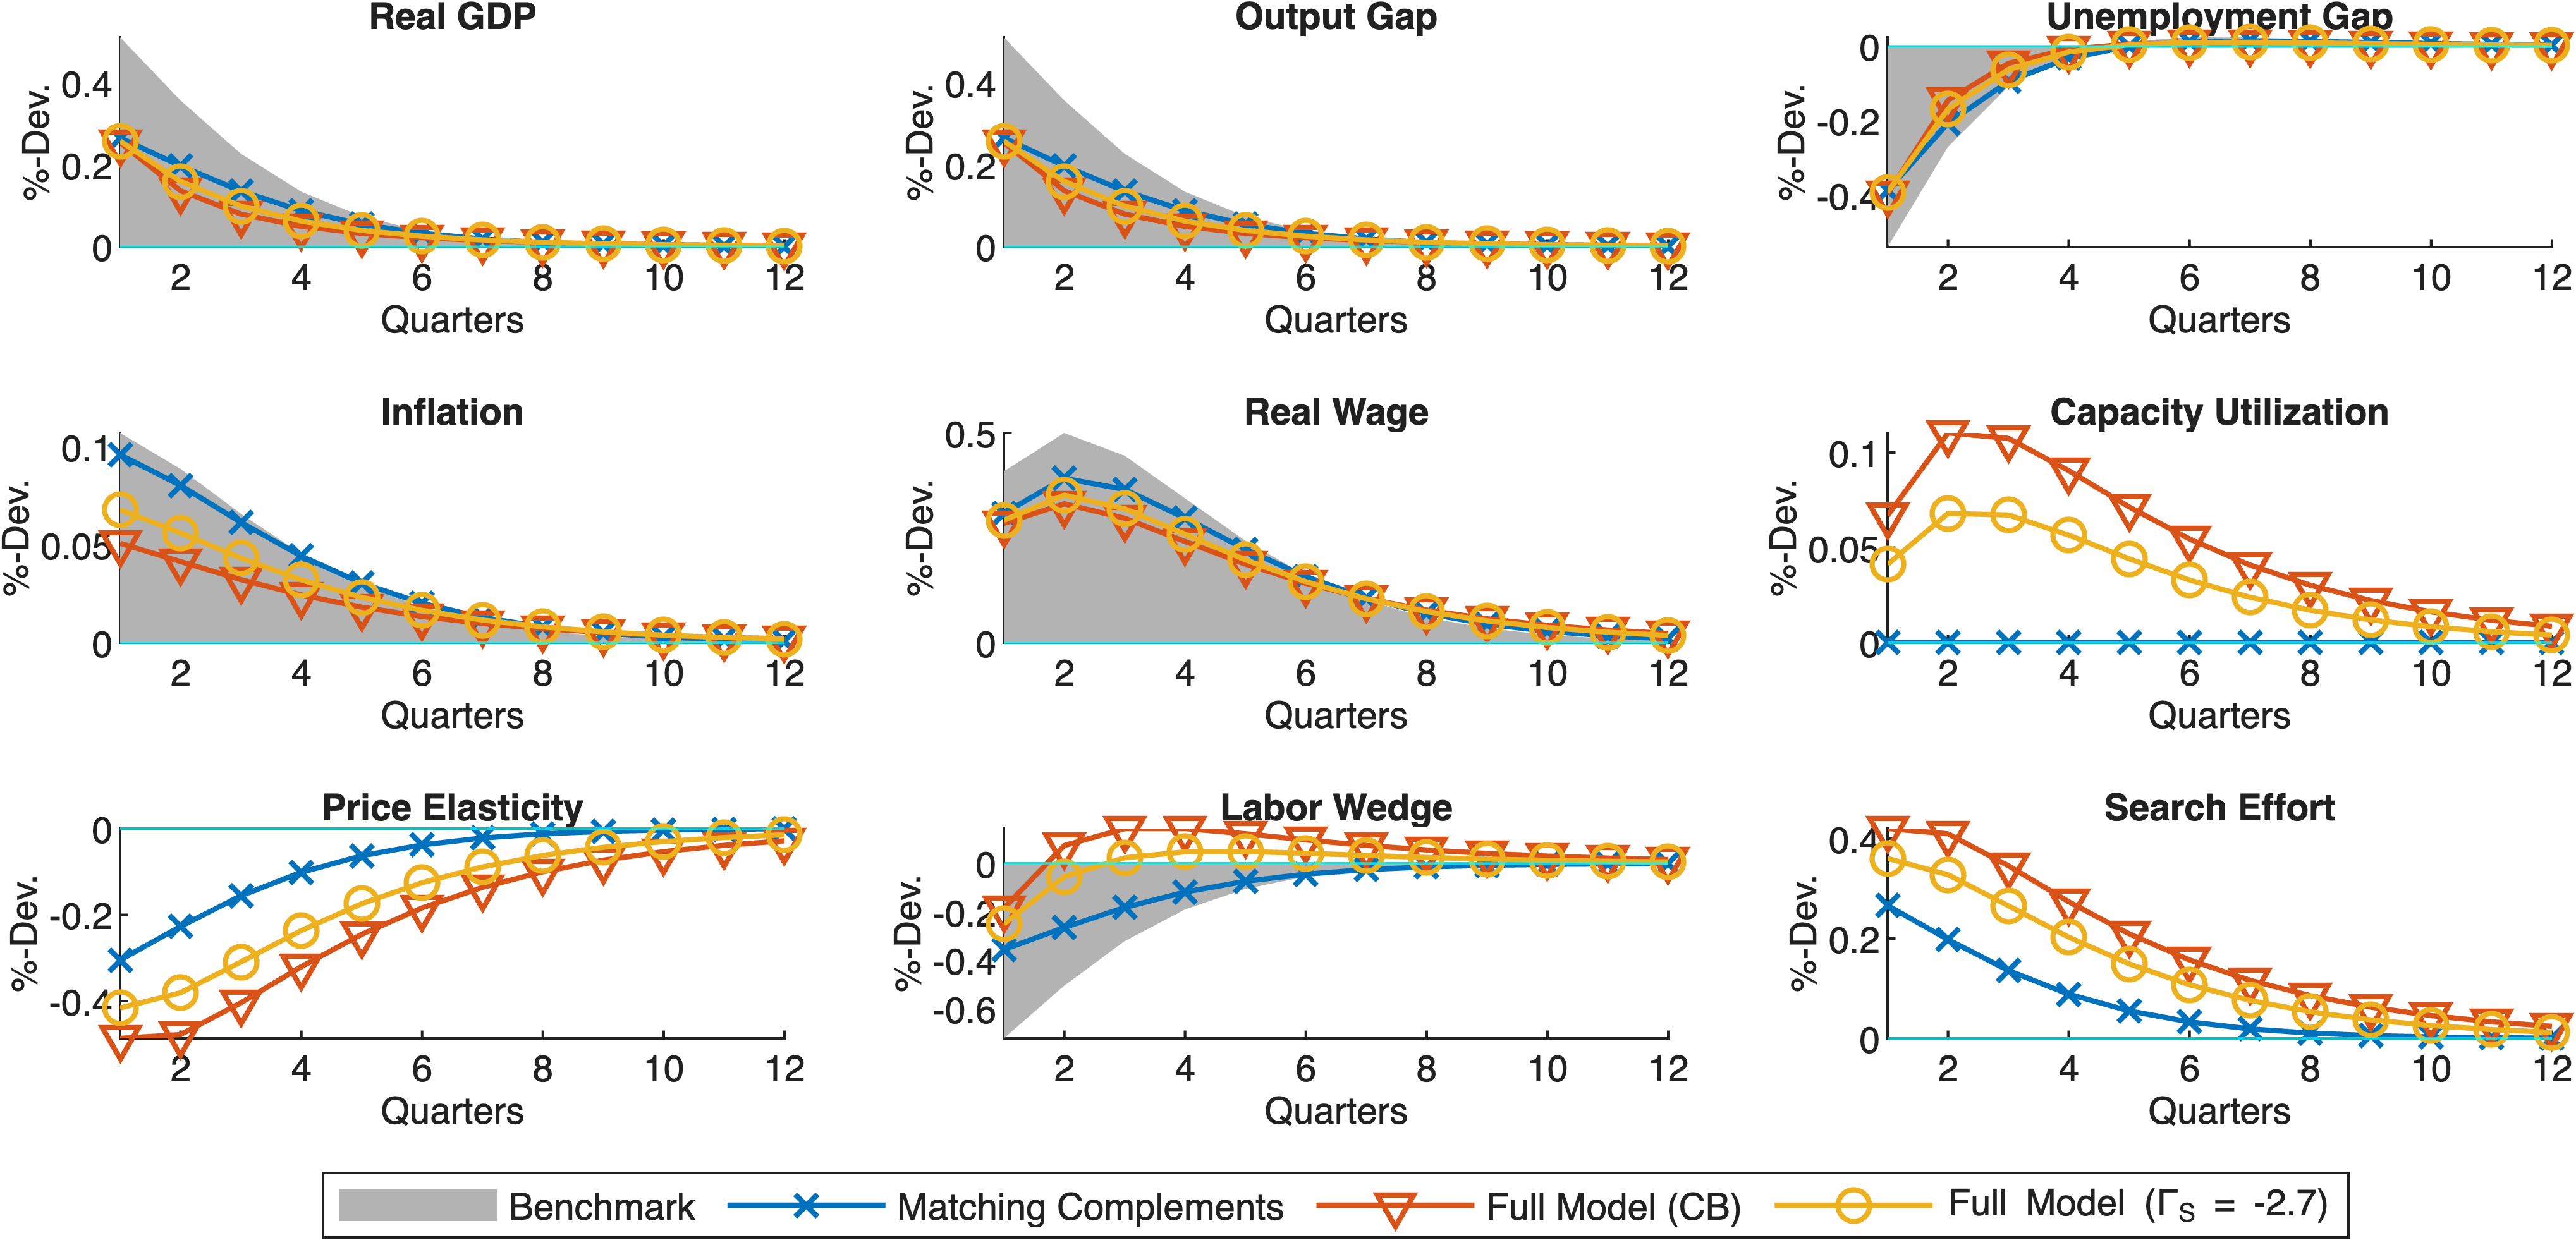
\includegraphics[width=\textwidth]{fig_5_irf_default_policy.png}%
	\vspace{-0.1in}%
	{\tiny \singlespacing NOTE: The figure shows IRFs to a one standard deviation expansionary monetary policy shock using the model presented in \cref{sec:model} and \cref{sec:dynamics}. The benchmark model follows \cref{prop:nosam}, the ''matching complements'' model sets $\Gamma_S = -\infty$, the CES model sets $\Gamma_S = -2.7$, the Cobb-Douglas model is calibrated as in \cref{tab:calibration}.\par}%
\end{figure}%
% CB GOODS MARKET SAM
Relaxing the matching inputs complementarity leads to a small quantitative decrease in the IRFs of real GDP, the output gap, the unemployment gap, and real wages. For $\Gamma_S = 0$, capacity utilization increases in search effort, which increases search prices and thus leads to a stronger decrease in the price elasticity and competition on the goods market. Inflation responses are smaller compared to the benchmark model which implies that the effect of capacity utilization on marginal costs dominates the effect of the price elasticity on demand. The initial response of the labor wedge is negative as low price elasticity and high aggregate demand decrease unemployment. As capacity utilization shows a hump-shaped and more persistent response than the price elasticity, it follows that the labor wedge deviates above its steady-state in transition. With strong substitutability of matching inputs, an expansionary monetary policy shock works more through higher utilization of existing production capacity rather than the expansion of it.\\%
% OVERALL POLICY SHOCK & CES FUNCTION
Overall, introducing goods market SaM with $\Gamma_S = 0$ makes the model in response to a monetary policy shock look more like a RBC model as output (gap), inflation, and labor deviations are smaller. Nominal shocks have a smaller impact on the economy. This pattern follows from procyclical capacity utilization amplifying countercyclical price elasticity which reduces competition on the goods market over the business cycle. Second moments of the simulation in \cref{tab:simul_stats} confirm those findings. For $\Gamma_S = -2.7$, the NK-SaM model converges back to the benchmark model but still shows a dampened response to this nominal shock. A lower substitutability of matching inputs allows to partially reconcile the NK-SaM model with a countercyclical labor wedge but at the cost of lower capacity utilization variation.%
%--------------------------------------------------------------------------
% Cost-Push Shocks in a Goods Market SaM Economy
%--------------------------------------------------------------------------
\subsection{Cost-Push Shocks in a Goods Market SaM Economy}%
% INTRODUCTION
The two goods market SaM shocks, $\hat{\psi}_t$ and $\hat{\mu}_{S,t}$, are natural candidates for cost-push shocks as they affect the non-pecuniary costs of the unobserved search effort. They exogenously change search prices and thus the price elasticity affecting the price-setting power of firms and are thus potential candidates for a micro-founded cost-push shock instead of the otherwise elusive markup shock modeled as exogenous variation to the elasticity of intratemporal substitution (EIS). \cite{schmitt2025hotelling} conduct a similar analysis with transportation costs in a NK model with spatial frictions.%
% Cost-Push Shocks in Comparison
%--------------------------------------------------------------------------
\paragraph{Cost-Push Shocks in Comparison}%
% INTRODUCTION
\Cref{fig:cost-push_comparison} shows IRFs to expansionary shocks\footnote{All three shocks are calibrated such that their initial expansionary real GDP response is roughly the same. With a shock persistence of $0.5$, all three shocks converge back to steady-state in about $4$ to $6$ quarters.} of the EIS, $\epsilon_t$, search effort disutility, $\mu_{S,t}$, and goods market matching efficiency, $\psi_t$. All three shocks qualify as cost-push shocks as they show IRFs of real GDP negatively correlated with IRFs of inflation while they do not affect the production process directly. The grey areas show the IRFs to an EIS shock in the benchmark model as in \cite{ireland_technology_2004}. The three curves show the cost-push shocks in the NK-SaM model as described above.\\%
% FIGURE
\begin{figure}[t]%
	\centering%
	\caption{IRFs to Different Cost-Push Shocks}\label{fig:cost-push_comparison}%
	\vspace{-0.1in}%
	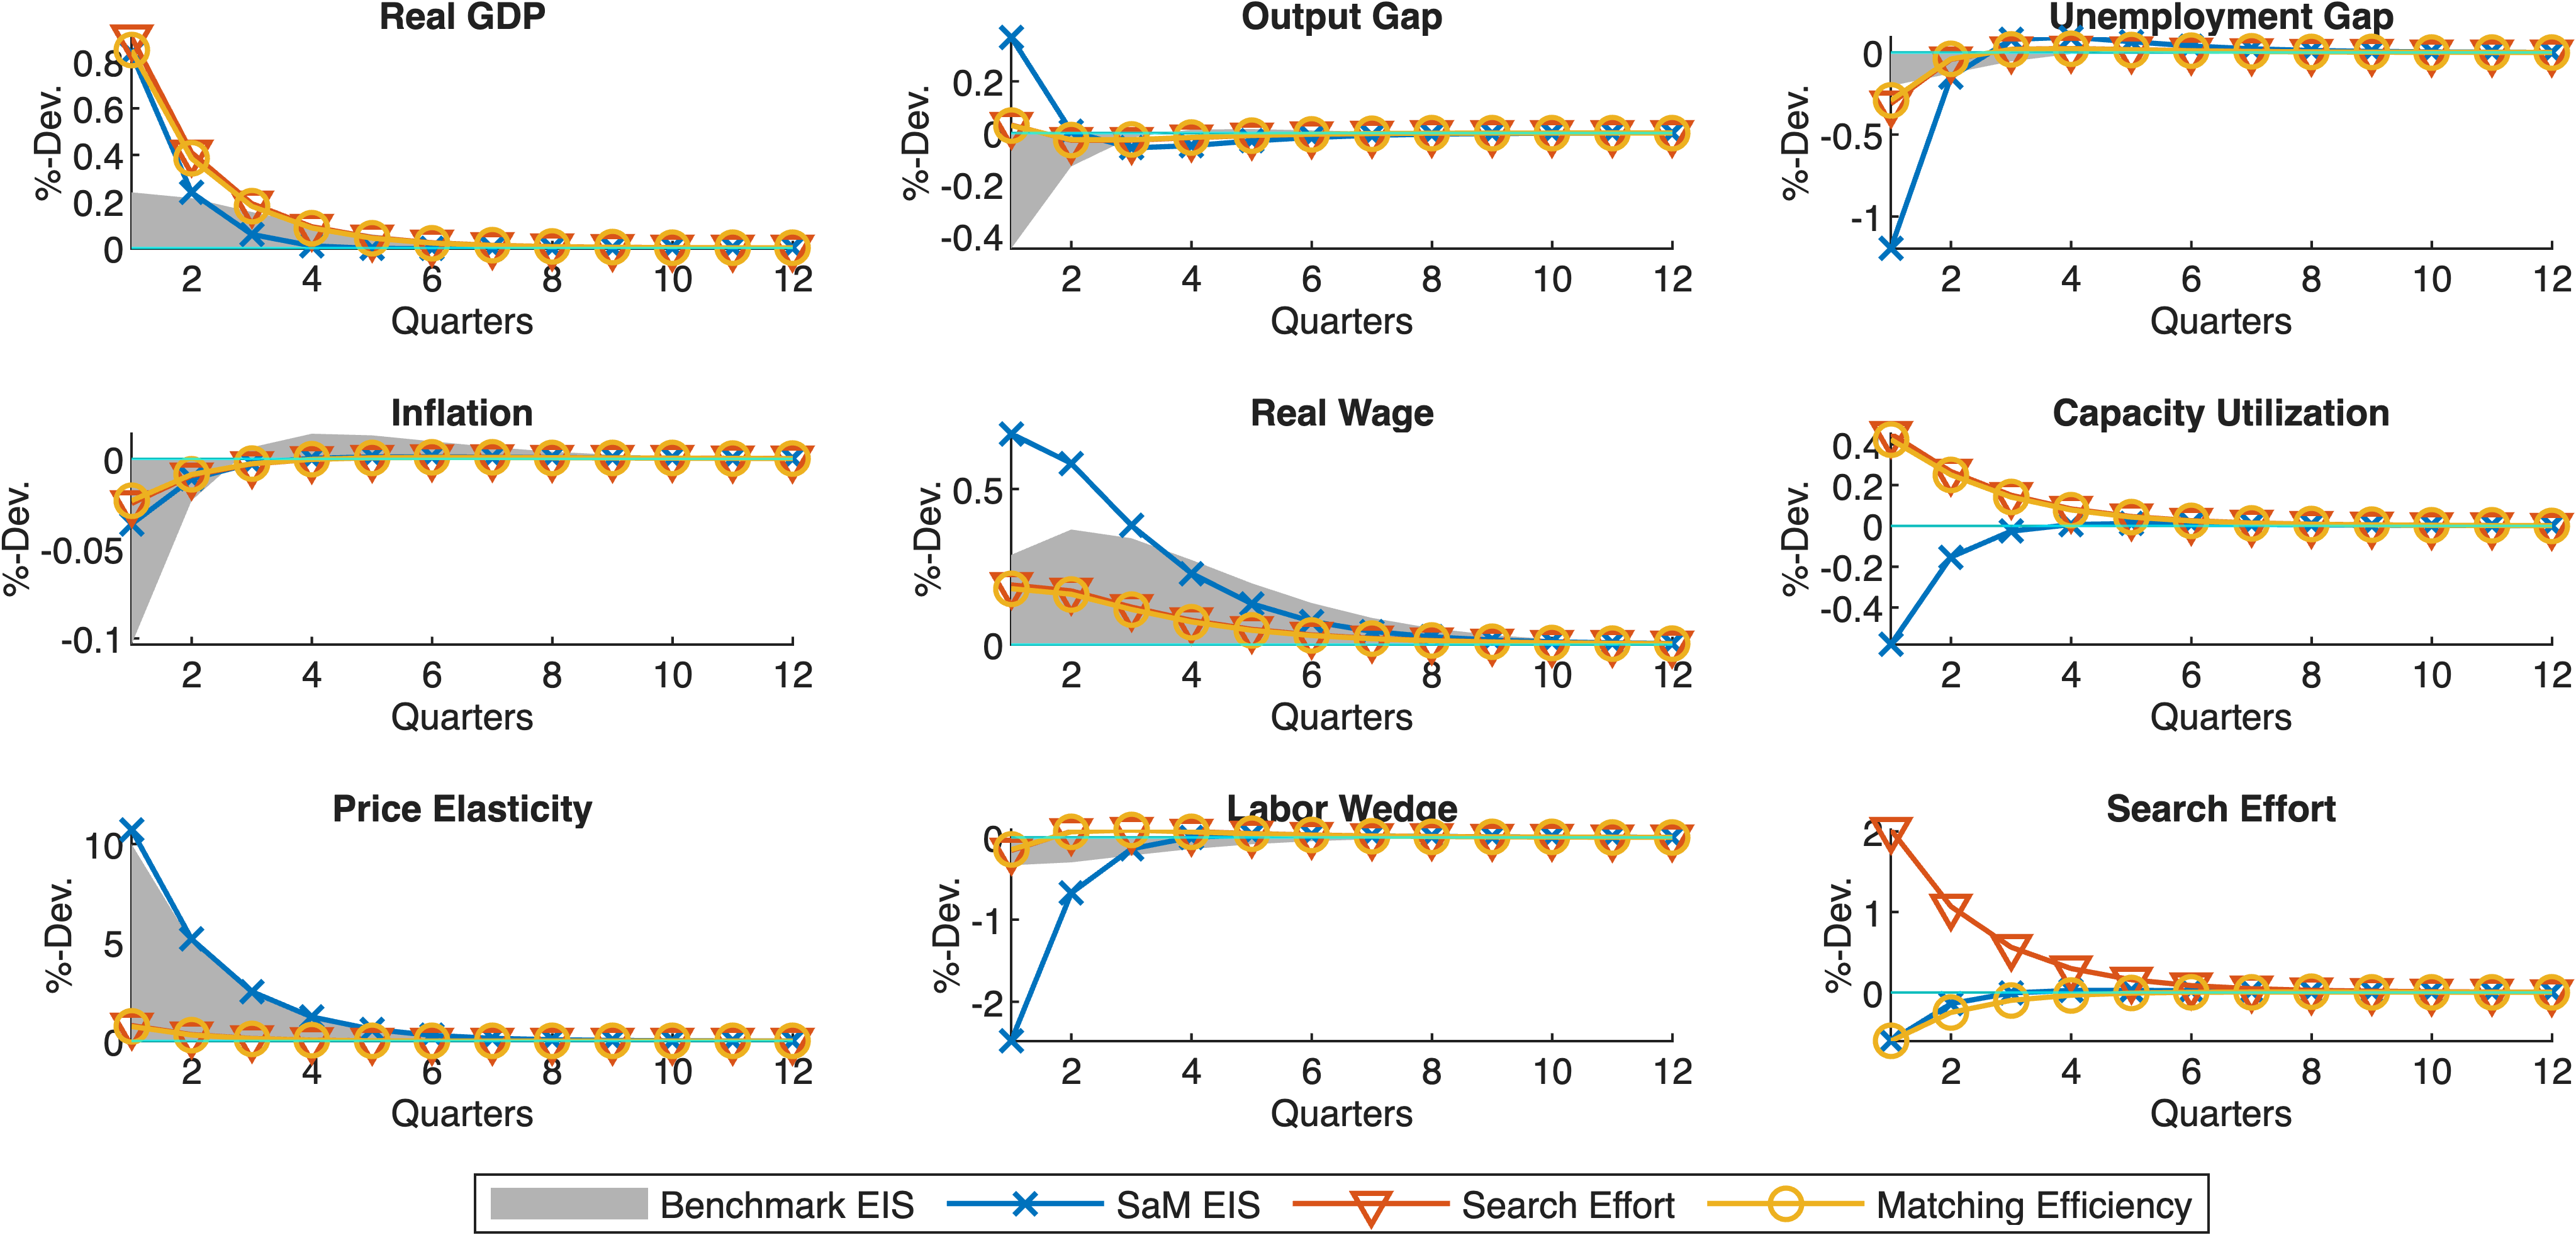
\includegraphics[width=\textwidth]{fig_6_irf_comparison_cost-push.png}%
	\vspace{-0.1in}%
	{\tiny \singlespacing NOTE: The figure shows IRFs to one standard deviation expansionary cost-push shocks using the model presented in \cref{sec:model} and \cref{sec:dynamics}. The benchmark model follows \cref{prop:nosam}, the Cobb-Douglas model is calibrated as in \cref{tab:calibration}. The shocks present exogenous variation in the elasticity of substitution (EIS), $\hat{\epsilon}_t$, in search effort, $\hat{\mu}_t$, and in matching efficiency, $\hat{\psi}_t$.\par}%
\end{figure}%
% COMPARISON: BENCHMARK NK MODEL SHOCK
The EIS shocks shows a $10\%$ increase in the price elasticity and thus in competition on the goods market in both the benchmark and the NK-SaM model by construction. Firms cut price in response which leads to higher aggregate demand and output. The inflation response is smaller in the NK-SaM model as capacity utilization (search effort) decreases which leads to an expansion of employment (lower labor wedge and higher real wages) and higher production capacity to attract additional demand in a more competitive environment. The incomplete pass-through of marginal costs to prices leads to a negative output gap in the benchmark model, while the capacity utilization channel in the NK-SaM model leads to a positive output gap\footnote{We calculate the output gap to the flexible price model. For the output gap of the efficient model (with no monopolistic competition), the output gap is procyclical for both the benchmark and the NK-SaM model.}. The procyclical output gap follows from capacity utilization entering the demand function. The shock induces a significant increase in competitiveness to the economy, but real GDP increases relatively little in the NK-SaM model and even less in the benchmark model.\\%
% GOODS MARKET SAM MODEL SHOCKS
In the NK-SaM model, search effort and matching efficiency shocks act as cost-push shocks. Targeting the same output response as for the EIS shock, we find similar deflation in the NK-SaM model. However, other variables show both qualitative and quantitative differences. The price elasticity and capacity utilization (search effort) are both procyclical. Both amplify the initial response through higher competition on the goods market, aggregate demand, and productivity. However, the IRFs of the price elasticity are significantly lower compared to the exogenous change of the EIS shock which resembles values closer to the data. As the increase in output works mainly through unobserved search effort, variation in labor market related-variables is significantly lower compared to the EIS shock. Second moments of the simulation in \cref{tab:simul_stats} confirm those findings. Low output gap variation implies low amplification of the exogenous shocks by the sticky price and wage assumptions in the NK-SaM model\footnote{We calculate the output gap to the flexible price model. If we assume no search friction and thus constant capacity utilization in the efficient model, then the output gap is procyclical for both shocks.}.\\%
% OVERALL
All three shocks show features of cost-push shocks. The NK-SaM model shows that such shocks can arise naturally from the demand side of the model. As there are clear interpretations of both demand side shocks, adding goods market SaM makes cost-push shocks in NK models ''less elusive'' \citep{schmitt2025hotelling}.%
% Search Effort Shock
%--------------------------------------------------------------------------
\paragraph{Search Effort Shock}
% GENERAL DESCRIPTION & TEXTBOOK DESCRIPTION & PERFECT COMPLEMENTS
We focus on the description of the search effort shock as the matching efficiency shock shows largely identical IRFs\footnote{Both NK-SaM shocks show identical IRFs. \cite{bai2025demand} show that the two shocks are identical up to the IRF of search effort. The same identity applies here as shown in \cref{fig:cost-push_comparison}. We focus on the search effort shock instead of the matching efficiency shock as it is in line with a procyclical search effort \citep{petrosky-nadeauShoppingTime2016}. While both shocks might explain part of the data, search effort shocks seem to be the more important shocks given shopping time data. Detailed IRFs for the matching efficiency shock can be found in \ref{sec:irf_add_cost-push}.}. \Cref{fig:irf_default_search_effort} shows IRFs to an expansionary search effort shock featuring the same models as in \cref{fig:irf_default_tfp}. All three versions of the NK-SaM model show a significant increase in real GDP. The case for $\Gamma_S = 0$ is given in the description of \cref{fig:cost-push_comparison}. For perfect matching input complements, the output (gap) IRFs show significantly larger deviations from steady-state as search effort does not substitute for supply. The price elasticity increases, inducing higher competition on the goods market and thus additional aggregate demand which is satisfied by higher labor supply. Real wages increase significantly while unemployment and the labor wedge decrease significantly. The expansion in output drives up marginal costs which leads to higher inflation. It follows that the search effort shock acts as an aggregate demand shock rather than a cost-push shock for perfect complement matching inputs as the increase in price elasticity is not balanced by an increase in capacity utilization. The specific workings of the goods market and unobserved search effort are thus crucial for the classification of this shock.\\%
% FIGURE
\begin{figure}[t]%
	\centering%
	\caption{Channel Comparison - IRFs to an Expansionary Search Effort Shock}\label{fig:irf_default_search_effort}%
	\vspace{-0.1in}%
	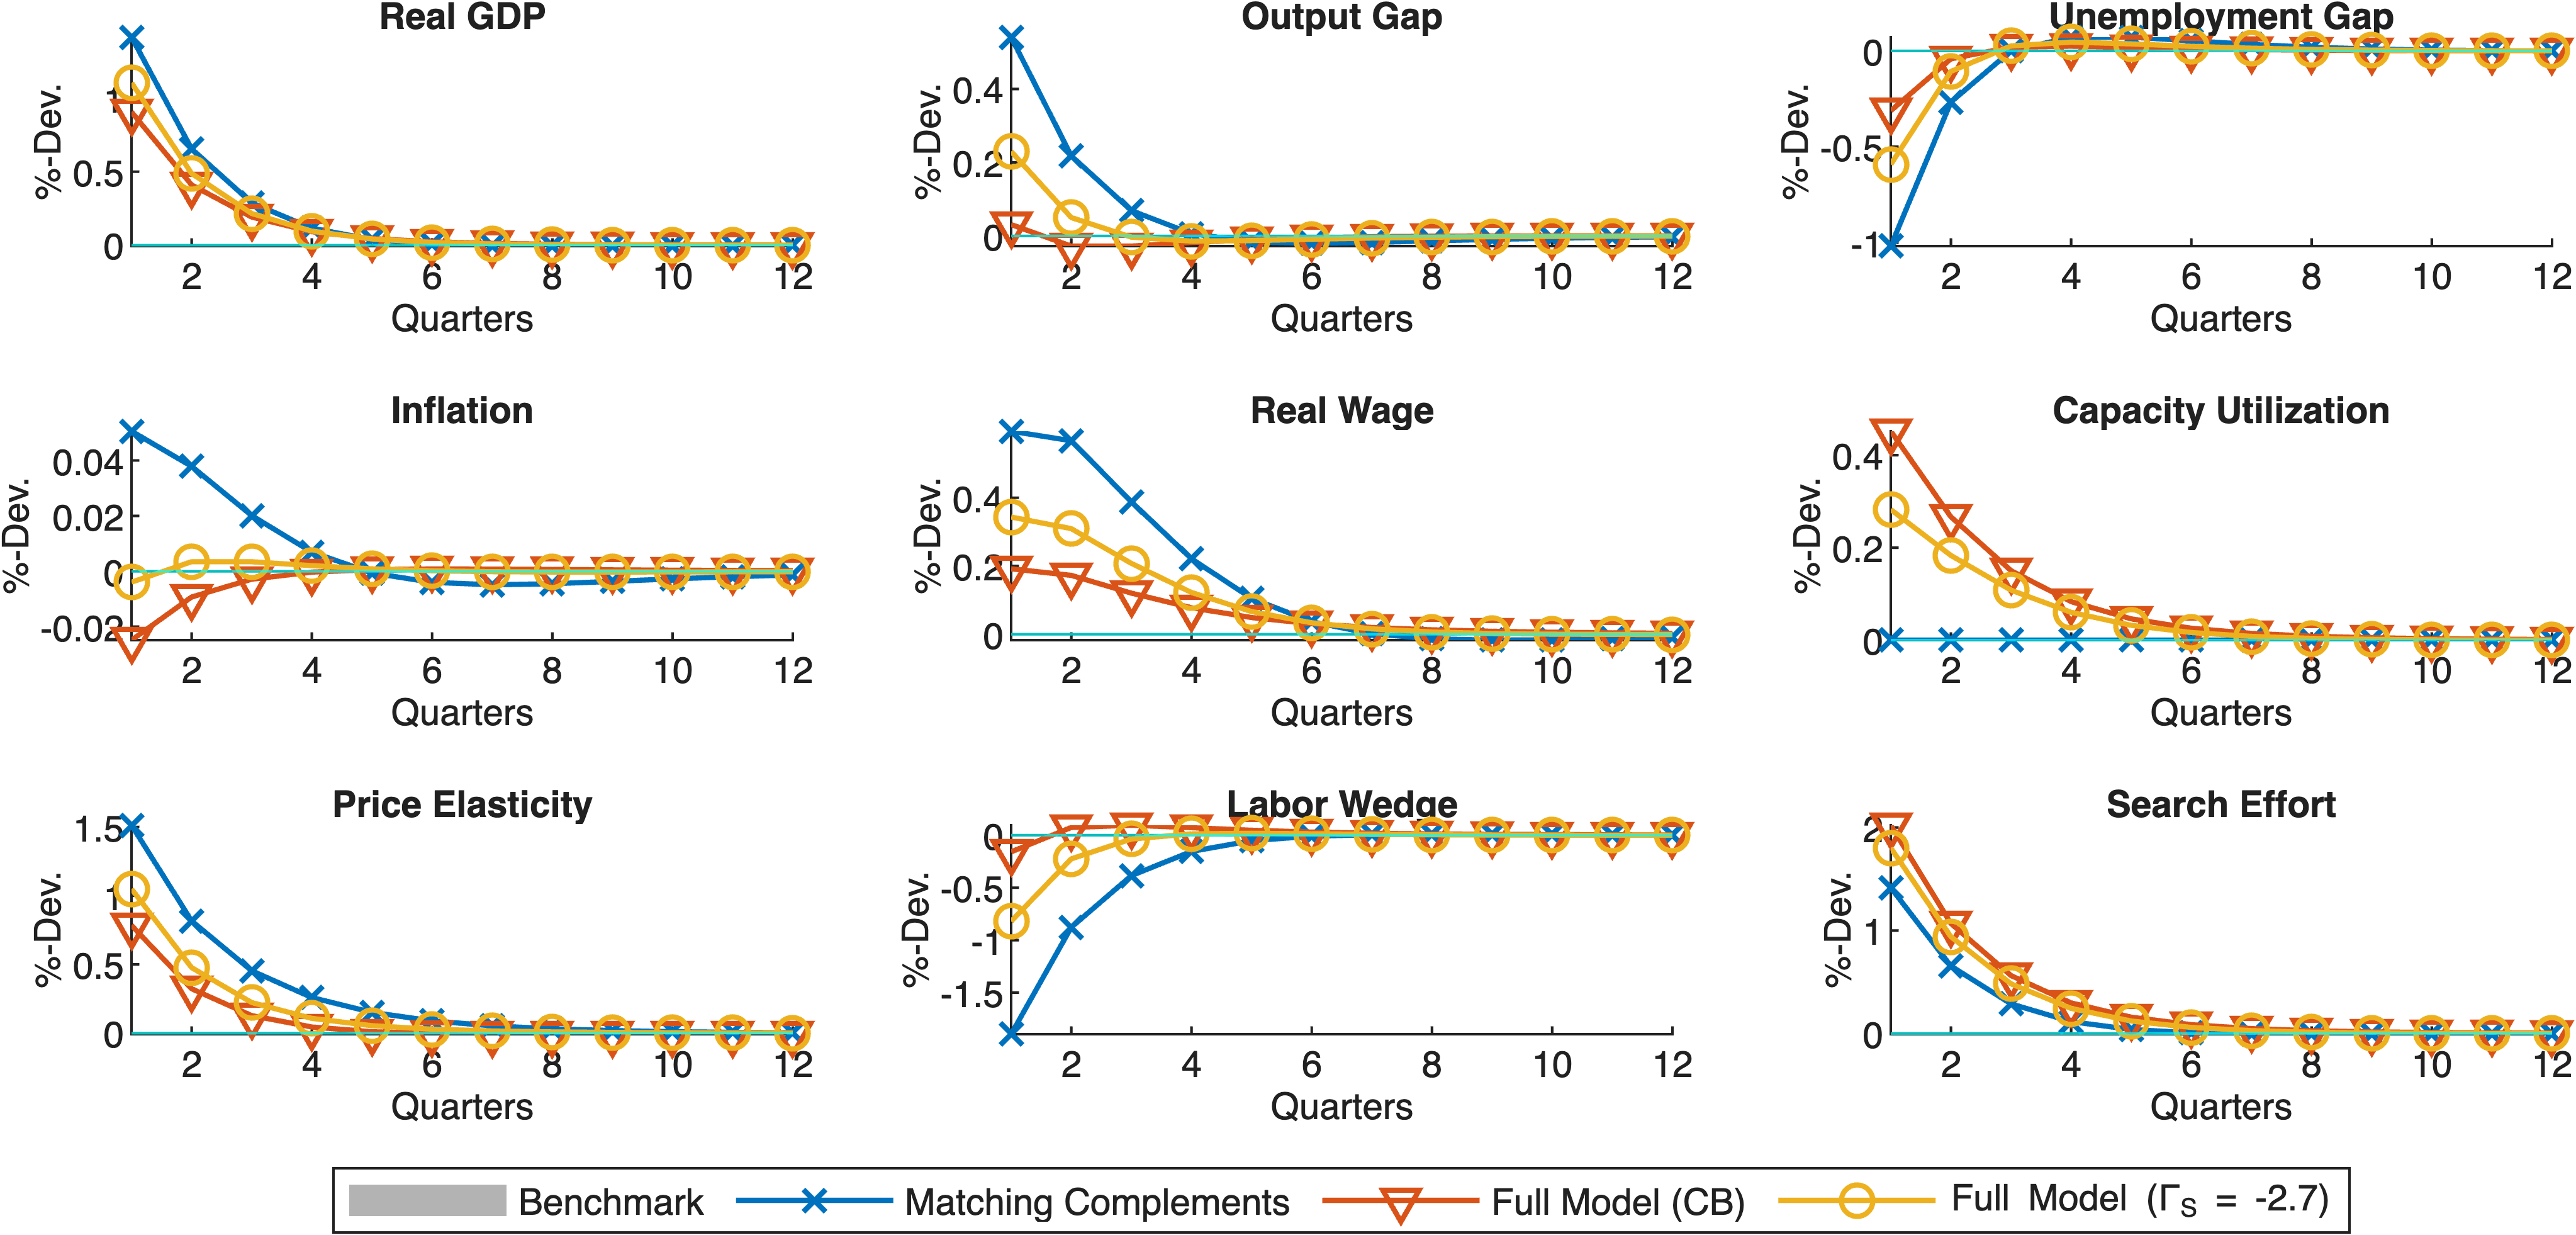
\includegraphics[width=\textwidth]{fig_7_irf_default_search.png}%
	\vspace{-0.1in}%
	{\tiny \singlespacing NOTE: The figure shows IRFs to a one standard deviation expansionary search effort shock using the model presented in \cref{sec:model} and \cref{sec:dynamics}. The benchmark model follows \cref{prop:nosam}, the ''matching complements'' model sets $\Gamma_S = -\infty$, the CES model sets $\Gamma_S = -2.7$, the Cobb-Douglas model is calibrated as in \cref{tab:calibration}.\par}%
\end{figure}%
% OVERALL
For $\Gamma_S = -2.7$, the IRFs are qualitatively identical to the Cobb-Douglas case although quantitatively less pronounced. The search effort shock still identifies as a cost-push shock. Overall, goods market SaM allows for a natural implementation of (demand side) cost-push shocks. This section has shown how the interaction of the \emph{price elasticity} and \emph{capacity utilization channels} is crucial for this interpretation. The search effort shock is a cost-push shock only if capacity utilization varies procyclically with search effort. The procyclical search effort elasticity found in \cite{petrosky-nadeauShoppingTime2016} hints in that direction.%
%--------------------------------------------------------------------------
% Statistics: Relative Standard Deviations and Correlations
%--------------------------------------------------------------------------
\subsection{Statistics: Relative Standard Deviations and Correlations}\label{sec:second_moments}%
% Statistics Table
%--------------------------------------------------------------------------
\begin{table}[t]%
	\begin{center}%
		\begin{footnotesize}%
			\caption{Relative Standard Deviations and Correlations of Model Simulations}\label{tab:simul_stats}%
			\begin{tabular}{l r r r r r r r r}%
				\hline%
				\textbf{Benchmark Model}& \multicolumn{2}{c}{Technology} & \multicolumn{2}{c}{Demand (Policy)} & \multicolumn{2}{c}{Cost-Push (EIS)} & \multicolumn{2}{c}{Search Effort}\\%
				Variable & Rel.Std. & Corr. & Rel.Std. & Corr. & Rel.Std. & Corr. & Rel.Std. & Corr.\\%
				\hline \hline%
				Output Gap & 0.28 & -0.67 & 1.00 & 1.00 & 1.39 & -0.76 & - & -\\%
				UE Gap & 0.08 & -0.42 & 0.96 & -0.95 & 0.73 & -0.90 & - & -\\%
				Inflation & 0.12 & -0.82 & 0.23 & 0.98 & 0.33 & -0.66 & - & -\\%
				Real Wage & 0.63 & 0.85 & 1.24 & 0.88 & 1.71 & 0.93 & - & -\\%
				Utilization & 0.00 & 0.00 & 0.00 & 0.00 & 0.00 & 0.00 & - & -\\%
				Marginal Cost & 0.81 & -0.76 & 1.24 & 0.88 & 1.71 & 0.93 & - & -\\%
				Price Elasticity & 0.00 & 0.01 & 0.00 & 0.00 & 32.62 & 0.92 & - & -\\%
				Labor Wedge & 1.11 & 0.92 & 1.41 & -1.00 & 1.41 & -1.00 & - & -\\%
				Search Effort & - & - & - & - & - & - & - & -\\%
				\hline \hline%
				\textbf{NK-SaM Model}& \multicolumn{2}{c}{Technology} & \multicolumn{2}{c}{Demand (Policy)} & \multicolumn{2}{c}{Cost-Push (EIS)} & \multicolumn{2}{c}{Search Effort}\\%
				Variable & Rel.Std. & Corr. & Rel.Std. & Corr. & Rel.Std. & Corr. & Rel.Std. & Corr.\\%
				\hline \hline%
				Output Gap & 0.08 & 0.28 & 1.00 & 1.00 & 0.45 & 0.94 & 0.06 & 0.30\\%
				UE Gap & 0.29 & -0.70 & 1.48 & -0.96 & 1.43 &-0.98 & 0.33 & -0.92\\%
				Inflation & 0.05 & -0.99 & 0.24 & 0.94 & 0.04 & -1.00 & 0.03 & -0.99\\%
				Real Wage & 0.58 & 0.91 & 1.82 & 0.80 & 1.06 & 0.82 & 0.27 & 0.90\\%
				Utilization & 0.57 & -1.00 & 0.61 & 0.67 & 0.70 & -1.00 & 0.53 & 0.99\\%
				Marginal Cost & 0.22 & -0.95 & 1.14 & 0.87 & 1.77 & 0.95 & 0.36 & -1.00\\%
				Price Elasticity & 0.52 & 0.95 & 2.67 & -0.87 & 13.56 & 0.97 & 0.86 & 1.00\\%
				Labor Wedge & 0.37 & 0.42 & 1.13 & -0.35 & 2.97 & -1.00 & 0.23 & -0.51\\%
				Search Effort & 0.42 & -0.95 & 2.29 & 0.87 & 0.72 & -1.00 & 2.30 & 1.00\\%
				\hline%
			\end{tabular}\\%
			{\tiny NOTE: The table shows simulated second moments for the benchmark and NK-SaM model. It shows relative standard deviations - standard deviation of each variable relative to standard deviation of real GDP - and correlations of each variable with real GDP. We consider each shock separately in the simulation.\par}%
		\end{footnotesize}%
	\end{center}%
\end{table}%
% OVERVIEW COMMON VARIABLES
Analyzing second moments as shown in \cref{tab:simul_stats} highlights the quantitative impact of goods market SaM for different shocks across models. The output gap varies little relative to real GDP in the NK-SaM model for technology, cost-push, and search effort shocks and shows a (small) positive instead of a negative correlation as in the benchmark model. The demand shock shows identical second moments across models as it does not induce variation in the flexible price model. The unemployment gap shows stronger variation relative to real GDP in the NK-SaM model with high relative standard deviation for demand and cost-push shocks. It is strongly countercyclical across models. Inflation variation relative to real GDP is lower for technology, cost-push, and search effort shocks in the NK-SaM model with a countercyclical pattern across models. Demand shocks show strong and positively correlated variation in inflation across models.\\%
% CAPACITY UTILIZATION AND SEARCH EFFORT
These changes in the second moments follow from variation of capacity utilization and the price elasticity in the NK-SaM model. Capacity utilization variation relative to real GDP is significant across shocks ($0.5$ to $0.6$), but smaller than its empirical counterpart at around $1.83$. It is procyclical for policy and search effort shocks while it is countercyclical for technology and cost-push shocks which allows to replicate the empirical correlation of $0.45$. This pattern also applies to search effort, which shows strong procyclical variation for policy and search effort shocks and somewhat smaller countercyclical variation for technology and cost-push shocks. This allows the model to match the procyclical search effort variation of $1.1$ to $1.6$ relative to real GDP in the data \citep{petrosky-nadeauShoppingTime2016}.\\%
% PRICE ELASTICITY
The ''super-elasticity'' of the price elasticity\footnote{The ''super-elasticity'' of the price elasticity is defined as the price elasticity of the price elasticity of demand \citep{klenow2016real}. It determines the change in the price elasticity as prices change.} is about $1$ to $4$ in the data \citep{beck2020price,dossche2010kinked} and slightly countercyclical. The model shows higher super-elasticities\footnote{We derive the super-elasticity in the model by dividing the relative standard deviation of the price elasticity by the relative standard deviation of inflation. Hence, the statistic shows by how much the price elasticity varies relative to a one percent change in inflation.} (in line with the slopes of \cref{sec:analysis}) between $10.4$ (technology) and $339$ (cost-push) with demand shocks ($11.1$) and search effort shocks ($28.67$) falling in-between. The demand shock is the only shock showing a countercyclical price elasticity with the other shocks showing a procyclical pattern. Overall, price elasticity is too volatile in the model with demand shocks coming closest to the empirical counterpart.\\%
% OVERALL, ROBUSTNESS, AND POLICY IMPLICATIONS
Overall, we find that the model is able to replicate the procyclical search effort found in the data. It creates procyclical capacity utilization and countercyclical price elasticity. In order to create this pattern, demand shocks must be a major business cycle driver. However, the model implies too low variation in capacity utilization and too high variation in the price elasticity compared to the data. One can improve upon that by choosing a lower $\nicefrac{\nu_S}{\nu_M}$ ratio as shown in \cref{tab:simul_stats_app}. However, its quantitative impact is overall small. The very low variation in the output gap implies that monetary policy should target the unemployment gap instead. As the correlation of the output gap with GDP is positive in the NK-SaM model it would also imply a policy tightening where inflation implies a cut in the interest rate. The correlation of the output gap with real GDP, however, is very sensitive to the calibration as shown in \cref{tab:simul_stats_app}.%
%--------------------------------------------------------------------------
% Robustness Analysis
%--------------------------------------------------------------------------
\subsection{Robustness Analysis}\label{sec:robust_sim}%
The model in this paper can be extended in several dimensions. Here, we present a few. Details on the model setup are given in \ref{sec:full_optimization} and results in \ref{sec:robust}.%
% Alternative Calibration
%--------------------------------------------------------------------------
\paragraph{Alternative Calibration (\ref{sec:calibration_add})}%
For $\gamma_S = 0.11$, the \emph{labor demand channel} dominates the \emph{price elasticity channel} which implies lower variation in price elasticity and capacity utilization as well as a countercyclical labor wedge. Calibrating $\nicefrac{\nu_S}{\nu_M} = 0.5$ amplifies the variation in capacity utilization but reduces the variation in the price elasticity, thus reduces the impact of goods market SaM on the IRFs as described by \cref{cor:agg_impact_sticky_price} (vice-versa for $\nicefrac{\nu_S}{\nu_M} = 1.5$). While calibrating a lower $\gamma_S$ with a lower $\nicefrac{\nu_S}{\nu_M}$ allows for a countercyclical labor wedge with significant variation of the goods market SaM channels, most of the literature hints at a higher $\gamma_S$ where the \emph{price elasticity channel} dominates \citep{bai2025demand,den2024role,michaillatAggregateDemandIdle2015,qiuProcyclicalProductivityNew2022}.%
% Alternative Preferences
%--------------------------------------------------------------------------
\paragraph{Alternative Preferences (\ref{sec:robust_hw} and \ref{sec:robust_ghh})}%
Using \cite{greenwoodInvestmentCapacityUtilization1988} preferences\footnote{We choose \cite{kingProductionGrowthBusiness1988} preferences as a baseline in this paper, as modeling unemployment following \cite{gali2011unemployment} requires intratemporal separability of the utility function determinants.} implies price elasticity and capacity utilization channels approximately $25\%$ smaller compared to our baseline NK-SaM model which translates to roughly the same decrease in slopes of the Euler equation\footnote{The impact of \cite{greenwoodInvestmentCapacityUtilization1988} preferences on the Euler equation slope is small in the NK-SaM model compared to the benchmark model (approximately $60\%$).}, Phillips curve, and real wage growth. The IRFs show that higher variation in output (gap) leads to an increase in the variation of capacity utilization and the price elasticity despite their smaller slopes. Using home production shows a similar impact as switching to \cite{greenwoodInvestmentCapacityUtilization1988} preferences - in line with \cite{lesterHomeProductionSticky2014}. Hence, it matters whether shopping time is allocated to home production or goods market SaM as it has the opposite impact on the properties of aggregate demand and supply.%
% Frictional Labor Markets
%--------------------------------------------------------------------------
\paragraph{Frictional Labor Markets (\ref{sec:robust_wages})}%
Setting $\kappa_W=0$ implies significantly larger variation ($25\%$-$50\%$) in the \emph{price elasticity} and \emph{capacity utilization channels} as unemployment is constant over the business cycle. It follows that output gap elasticity of the Euler equation is lower, price-setting is more flexible, and real wage growth is larger. It dampens the impact of goods market SaM following technology shocks as wages (thus labor and production capacity) increase more. For demand and search shocks we find the opposite impact as larger wage growth cuts off labor demand. Adding hours adjustment costs\footnote{Quadratic hours adjustment costs act as a proxy for labor market SaM \citep{blanchardLaborMarketsMonetary2010} while keeping the model structure relatively simple.} \citep{lechthalerQuadraticLaborAdjustment2013} amplifies the IRFs along the lines of sticky wages. Having both adds up their effects as the trade-off between market labor and search effort is further altered.%
% Capital in Production
%--------------------------------------------------------------------------
\paragraph{Capital in Production (\ref{sec:robust_capital})}%
Adding capital and capital utilization similar to \cite{christianoDSGEModelsMonetary2010} shows a small qualitative and quantitative impact on the NK-SaM model. The IRFs show more persistent variation. Capacity utilization variation decreases slightly for technology and demand shocks, while it increases slightly for search effort shocks. Price elasticity variation is mostly unchanged with the exception of a lower persistence following a technology shock. The most salient impact is the labor wedge becoming acyclical which allows to easier reconcile search effort patterns with a countercyclical labor wedge. Adding capital has a smaller impact on the NK-SaM than the benchmark model as household time allocation is more important due to the search effort margin.%
% Long-Term Goods Market SaM
%--------------------------------------------------------------------------
\paragraph{Long-Term Goods Market SaM (\ref{sec:robust_longterm_sam})}%
Adding firm inventories \citep{den2024role} shows a quantitatively small impact as inventory holdings are costly and available only for industry sectors which comrpise about one third of overall GDP. Adding goods market long-term contracts \citep{mathaSearchProductMarket2011,michaillatAggregateDemandIdle2015} with an average contract length of one year shows significant impact on the goods market SaM channels. Lower search costs per unit traded imply lower variation in the price elasticity and capacity utilization, thus the IRFs converge to the benchmark model as contract length expands. The search effort shock shows a smaller impact as the search frictions it alleviates is smaller. The reduction in search frictions leads to a general increase in inflation variation. Therefore, the impact of goods market SaM depends on continuous and significant search costs on the goods market which are alleviated by long-term contracts.%
%--------------------------------------------------------------------------
% 7. CONCLUSION
%--------------------------------------------------------------------------
%--------------------------------------------------------------------------
% 7. DISCUSSION AND CONCLUDING REMARKS
%--------------------------------------------------------------------------
\section{Discussion and Concluding Remarks}\label{sec:conclusion}%
%  MODEL OVERVIEW / MAIN RESULTS
This paper extends the NK model with home production to include procyclical household shopping effort via goods market SaM, inducing a state-dependent price elasticity of demand amplified by endogenous variation in capacity utilization. Goods market SaM reduces long-run GDP by reducing labor demand, labor supply, and the utilization of the resulting production capacity while making price-setting \emph{$12\%$ more flexible} and aggregate demand \emph{up to ten times less responsive} to interest rate changes. Hitting a given output-gap target requires larger interest-rate moves when goods market SaM is active as interest rates do not directly affect search price growth. Therefore, separating shopping time from home production and adding it via goods market SaM changes the sign of its impact on aggregate supply and demand.\\%
% SIMULATION / DISCUSSION - MONETARY POLICY
Simulation results confirm a muted output gap responses and weakened monetary policy transmission in general equilibrium. The level of competition on the goods market varies in the state-dependent price elasticity of demand. It follows that the model aligns with RBC-like output (gap) and employment dynamics yet preserves empirical inflation responsiveness to the labor share. Cost-push shocks arise naturally from the demand side as unobserved search effort changes lead to an increase in prices while aggregate demand decreases. In fact, as the price elasticity is endogenous, all shocks have a cost-push like component. These changes in the volatility of monetary policy targets and the effectiveness of policy transmission affect optimal monetary policy not only for monetary shocks, but also for other business cycle shocks warranting a more detailed (optimal) monetary policy analysis.\\%
% DISCUSSION - SEARCH COSTS / PREFERENCES / LABOR WEDGE
The model is capable of reproducing empirical variation in shopping time and significant procyclical variation in capacity utilization. However, it does not match the high variation of capacity utilization in the data and creates a trade-off with matching the countercyclical labor wedge. However, one can improve upon that trade-off by introducing capital and labor market frictions into the model. Hence, a natural next step is to set up this channel in a medium-sized DSGE model and estimate it using Bayesian estimation. As there is no quarterly data on shopping time, capacity utilization can act as a proxy in the estimation.\\%
% OVERALL - CLOSING SENTENCES
Overall, the framework highlights how pecuniary and non-pecuniary consumption costs shape inflation, output dynamics, and monetary policy over the business cycle. It invites further work on the impact of the goods market structure on NK models. Extending it to include household heterogeneity is likely to be especially fruitful as time allocation shows significant heterogeneity in the data.%
%--------------------------------------------------------------------------
% STATEMENTS AND LITERATURE
%--------------------------------------------------------------------------
\newpage%
\begin{small}%
	% AI STATEMENT
	\section*{Declaration of Generative AI and AI-Assisted Technologies in the Writing Process}%
	\noindent During the preparation of this work the author used ChatGPT in order to improve the readability and language of the manuscript. After using this service, the author reviewed and edited the content as needed and takes full responsibility for the content of the published article.%
\end{small}%
% REFERENCE LIST
\bibliographystyle{elsarticle-harv}%
\bibliography{references_nksam}%
%--------------------------------------------------------------------------
% APPENDIX
%--------------------------------------------------------------------------
\newpage%
\appendix%
%--------------------------------------------------------------------------
% A. APPENDIX
%--------------------------------------------------------------------------
%--------------------------------------------------------------------------
% Complete Model Setup and Derivation of First-Order Conditions
%--------------------------------------------------------------------------
\section{Complete Model Setup and Derivation of First-Order Conditions}\label{sec:full_optimization}%
%--------------------------------------------------------------------------
% Goods Market Setup
%--------------------------------------------------------------------------
\subsection{Goods Market Setup}%
\begin{small}%
	\paragraph{Goods market law of motion}%
	\begin{align}%
	 	T_t(i,j) \; = & \; \left(1-\delta_T\right) T_{t-1}(i,j) + m_t(i,j)\label{eq:appendix_matching}%
	\end{align}%
	\paragraph{Goods market matching function}%
	\begin{align}%
		m_t(i,j) \; = & \; \psi_{t} \left[ \gamma_S H_{S,t}(i,j)^{\Gamma_S} + (1-\gamma_S) S_t(i,j)^{\Gamma_S} \right]^{\frac{1}{\Gamma_S}}%
	\end{align}%
	\paragraph{Goods market tightness}%
	\begin{align}%
		x_t(i,j) \; = & \; \frac{H_{S,t}(i,j)}{S_t(i,j)} \; = \; \frac{q_t(i,j)}{f_t(i,j)}\label{eq:appendix_tightness}%
	\end{align}%
	\paragraph{Goods market matching probabilities}%
	\begin{align}%
	 	f_t(i,j) \; = & \; \frac{m_t(i,j)}{H_{S,t}(i,j)} \; = \; \psi_{t} \left[ \gamma_S + (1-\gamma_S) x_t(i,j)^{-\Gamma_S} \right]^{\frac{1}{\Gamma_S}}\\%
	 	q_t(i,j) \; = & \; \frac{m_t(i,j)}{S_t(i,j)} \; = \; \psi_{t} \left[ \gamma_S x_t(i,j)^{\Gamma_S} + (1-\gamma_S) \right]^{\frac{1}{\Gamma_S}}%
	\end{align}%
\end{small}%
% Labor Union: Aggregator and Quadratic Hours Adjustment Cost
%--------------------------------------------------------------------------
\pagebreak%
\subsection{Labor Union: Aggregator and Quadratic Hours Adjustment Cost}%
\begin{small}%
	\paragraph{Optimization problem of the labor union}%
 	\begin{align*}%
		 \mathcal{L} = \max_{H_{M,t}, H_{M,t}(i), H_{M,t}(j)} \mathbb{E}_0 \sum_{t=0}^{\infty} \beta_{0,t} & \biggl\{ \left[W_t \int_0^1 H_{M,t}(i) di - \int_0^1 W_t(j)H_{M,t}(j) dj - c_{HM,t} W_t H_{M,t} \right]\\%
		 & - \Omega_{1,t} \left[H_{M,t} - \left( \int_0^1 H_{M,t}(j)^{\frac{\epsilon_W-1}{\epsilon_W}} dj \right)^{\frac{\epsilon_W}{\epsilon_W-1}} \right]\\%
		 & - \Omega_{2,t} \left[H_{M,t} - \int_0^1 H_{M,t}(i) di\right] \biggr\}%
 	\end{align*}%
 	\paragraph{First-order condition}%
 	\begin{align}%
		W_t(j) \left(\frac{H_{M,t}(j)}{H_{M,t}}\right)^{\frac{1}{\epsilon_W}} \; = & \; W_t \phi_{HM,t},\\\label{eq:appendix_labor_demand}%
		\phi_{HM,t} \; = & \; 1 - c_{HM,t} - c^{\prime}_{HM,t} + \mathbb{E}_t \beta_{t,t+1} \frac{W_{t+1}}{W_t} \left(\frac{H_{M,t+1}}{H_{M,t}}\right) c^{\prime}_{HM,t+1},\\%
		c_{HM,t} \; = & \; \frac{\kappa_{HM}}{2} \left(\frac{H_{M,t}}{H_{M,t-1}}-1\right)^2,\\%
		c^{\prime}_{HM,t} \; = & \; \kappa_{HM} \left(\frac{H_{M,t}}{H_{M,t-1}}-1\right)\frac{H_{M,t}}{H_{M,t-1}}.%
	\end{align}%
\end{small}%
% Household Optimization
%--------------------------------------------------------------------------
\pagebreak%
\subsection{Optimization Problem: Household of Type \textit{j}}%
\begin{small}%
	% Lagrange maximization problem
	\subsubsection{Lagrange Maximization Problem (Households)}%
	\vspace{-0.2in}%
	\begin{align*}%
		\mathcal{L} = & \max_{\substack{C_t(i,j), D_t(i,j), H_t(i,j), W_t(i,j),\\B_t(i,j), K_t(i,j), I_t(i,j)}} \mathbb{E}_0 \sum_{t=0}^{\infty} \beta^t \biggl\{ \mathbb{U} \biggl(C_t(j), H_{S,t}(i,j), H_{H,t}(j), H_{M,t}(j)\biggr)\\%
		& - \lambda_{1,t} \biggl[ B_t(j) - \left(1+r_{t-1}\right) B_{t-1}(j) + \int_0^1 P_t(i,j) T_t(i,j) di\\%
		& \quad \quad \quad \quad - \Bigl(1-c_{W,t}(j)\Bigr) W_t(j) H_{M,t}(j) - P_{t} r_{K,t} e_{M,t}(j) K_{M,t-1}(j) - \Pi_{t} \biggr]\\%
		& - \lambda_{2,t} \biggl[ C_t(j) - \Bigl( \gamma_H C_{H,t}(j)^{\Gamma_H} + \left(1-\gamma_H\right) C_{M,t}(j)^{\Gamma_H} \Bigr)^{\frac{1}{\Gamma_H}} \biggr]\\%
		& - \int_0^1 \lambda_{3,t}(i,j) \biggl[ T_t(i,j) - \left(1-\delta_T\right) T_{t-1}(i,j) - f_t(i,j) H_{S,t}(i,j) \biggr] di\\%
		& - \lambda_{4,t} \biggl[ H_{M,t}(j) - \left(\frac{W_t^*}{W_{t}(j)}\phi_{HM,t}\right)^{\epsilon_W} H_{M,t} \biggr]\\%
		& - \lambda_{5,t} \biggl[ K_{M,t}(j) - \Bigl( 1 - \delta_M \left(e_{M,t}(j)\right) \Bigr)  K_{M,t-1}(j) - \Bigl(1-c_{MI,t}(j)\Bigr) I_{M,t}(j) \biggr]\\%
		& - \lambda_{6,t} \biggl[ K_{H,t}(j) - \Bigl( 1 - \delta_H \left(e_{H,t}(j)\right) \Bigr)  K_{H,t-1}(j) - \Bigl(1-c_{HI,t}(j)\Bigr) I_{H,t}(j) \biggr]\\%
		& - \lambda_{7,t} \biggl[ \left(\int_0^1 T_t(i,j)^{\frac{\epsilon_t-1}{\epsilon_t}} di \right)^{\frac{\epsilon_t}{\epsilon_t-1}} - C_{M,t}(j) - I_{M,t}(j) - I_{H,t}(j) \biggr] \biggr\},%
	\end{align*}%
	where%
	\begin{align*}%
		C_{H,t}(j) \; = & \; H_{H,t}(j)^{1-\alpha_H} \Bigl[ e_{H,t}(j)K_{H,t-1}(j)\Bigr]^{\alpha_H},
	\end{align*}%
	and it is assumed that the no-Ponzi scheme condition $\lim_{T\rightarrow\infty} \mathbb{E}_t B_T(j) \geq 0$ holds.%
\end{small}%
% Functional Forms
%--------------------------------------------------------------------------
\pagebreak%
\subsubsection{Functional Forms (Households)}%
\begin{small}%
% Cost functions
\paragraph{Cost functions}%
Adjustment costs and capital depreciation are described by:%
\begin{align*}%
	c_{W,t}(j) \; = & \; \frac{\kappa_W}{2} \left(\frac{W_t(j)}{W_{t-1}(j)}-1\right)^2\\%
	\delta_{M,t}(j) \; = & \; \delta_{M1} + \frac{\delta_{M2} \delta_{M3}}{2} \Bigl( e_{M,t}(j)-1 \Bigr)^2 + \delta_{M3} \Bigl( e_{M,t}(j)-1 \Bigr)\\%
	\delta_{H,t}(j) \; = & \; \delta_{H1} + \frac{\delta_{H2} \delta_{H3}}{2} \Bigl( e_{H,t}(j)-1 \Bigr)^2 + \delta_{H3} \Bigl( e_{H,t}(j)-1 \Bigr)\\%
	c_{MI,t}(j) \; = & \; \frac{\kappa_{MI}}{2}\left(\frac{I_{M,t}(j)}{I_{M,t-1}(j)}-1\right)^2\\%
	c_{HI,t}(j) \; = & \; \frac{\kappa_{HI}}{2}\left(\frac{I_{H,t}(j)}{I_{H,t-1}(j)}-1\right)^2%
\end{align*}%
% Utility function
\paragraph{Utility function} Alternative setups of utility functional form are described by:\\%
\textbf{\cite{greenwoodInvestmentCapacityUtilization1988} preferences} (aggregate/firm-specific convexity in search disutility):%
\begin{align}%%
	\mathbb{U}_t(i,j) \; = & \; \frac{\left[ C_t(j) - \mu_{S,t} \frac{\int_0^1 H_{S,t}(i,j)^{1+\nu_S} di}{1+\nu_S} - \mu_H \frac{H_{H,t}(j)^{1+\nu_H}}{1+\nu_H} - \mu_M \frac{H_{M,t}(j)^{1+\nu_M}}{1+\nu_M} \right]^{1-\sigma}}{1-\sigma}\\%
	\mathbb{U}_t(i,j) \; = & \; \frac{\left[ C_t(j) - \mu_{S,t} \frac{\left(\int_0^1 H_{S,t}(i,j) di\right)^{1+\nu_S}}{1+\nu_S} - \mu_H \frac{H_{H,t}(j)^{1+\nu_H}}{1+\nu_H} - \mu_M \frac{H_{M,t}(j)^{1+\nu_M}}{1+\nu_M} \right]^{1-\sigma}}{1-\sigma}%
\end{align}%
\textbf{\cite{kingProductionGrowthBusiness1988} preferences} (aggregate/firm-specific convexity in search disutility):%
\begin{align}%%
	\mathbb{U}_t(i,j) \; = & \; \frac{C_t(j)^{1-\sigma}}{1-\sigma} - \mu_{S,t} \frac{\left(\int_0^1 H_{S,t}(i,j) di\right)^{1+\nu_S}}{1+\nu_S} - \mu_H \frac{H_{H,t}(j)^{1+\nu_H}}{1+\nu_H} - \mu_M \frac{H_{M,t}(j)^{1+\nu_M}}{1+\nu_M}\\%
	\mathbb{U}_t(i,j) \; = & \; \frac{C_t(j)^{1-\sigma}}{1-\sigma} - \mu_{S,t} \frac{\int_0^1 H_{S,t}(i,j)^{1+\nu_S} di}{1+\nu_S} - \mu_H \frac{H_{H,t}(j)^{1+\nu_H}}{1+\nu_H} - \mu_M \frac{H_{M,t}(j)^{1+\nu_M}}{1+\nu_M}%
\end{align}%
% First-order conditions:
\textbf{FOC composite consumption} (aggregate/firm-specific convexity in search disutility):%
\begin{align}%
	\frac{\partial \mathbb{U}_t(i,j)}{\partial C_t(j)} \; = & \; \left[ C_t(j) - ghh \left( \mu_{S,t} \frac{H_{S,t}(j)^{1+\nu_S}}{1+\nu_S} + \mu_H \frac{H_{H,t}(j)^{1+\nu_H}}{1+\nu_H} + \mu_M \frac{H_{M,t}(j)^{1+\nu_M}}{1+\nu_M} \right) \right]^{-\sigma}\\%
	\begin{split}%
		\frac{\partial \mathbb{U}_t(i,j)}{\partial C_t(j)} \; = & \; \left[ C_t(j) - ghh \left( \mu_{S,t} \frac{\int_0^1 H_{S,t}(i,j)^{1+\nu_S} di}{1+\nu_S} \right. \right.\\%
		& \; \left. \left. \quad \quad \quad \quad \quad \quad \quad + \mu_H \frac{H_{H,t}(j)^{1+\nu_H}}{1+\nu_H} + \mu_M \frac{H_{M,t}(j)^{1+\nu_M}}{1+\nu_M} \right) \right]^{-\sigma}%
	\end{split}%
\end{align}%
\textbf{FOC search effort} (aggregate/firm-specific convexity in search disutility):%
\begin{align}%
	\frac{\partial \mathbb{U}_t(i,j)}{\partial H_{S,t}(i,j)} \; = & \; \left[ ghh \frac{\partial \mathbb{U}_t(i,j)}{\partial C_t(j)}+ \left(1-ghh\right) \right] (-\mu_{S,t}) \left(\int_0^1 H_{S,t}(i,j) di\right)^{\nu_S}\\%
	\frac{\partial \mathbb{U}_t(i,j)}{\partial H_{S,t}(i,j)} \; = & \; \left[ ghh \frac{\partial \mathbb{U}_t(i,j)}{\partial C_t(j)}+ \left(1-ghh\right) \right] (-\mu_{S,t}) H_{S,t}(i,j)^{\nu_S}%
\end{align}%
\textbf{FOCs home and market labor supply:}%
\begin{align}%
	\frac{\partial \mathbb{U}_t(i,j)}{\partial H_{H,t}(j)} \; = & \; \left[ ghh \frac{\partial \mathbb{U}_t(i,j)}{\partial C_t(j)}+ \left(1-ghh\right) \right] (-\mu_H) H_{H,t}(j)^{\nu_H}\\%
	\frac{\partial \mathbb{U}_t(i,j)}{\partial H_{M,t}(j)} \; = & \; \left[ ghh \frac{\partial \mathbb{U}_t(i,j)}{\partial C_t(j)}+ \left(1-ghh\right) \right] (-\mu_M) H_{M,t}(j)^{\nu_M}%
\end{align}%
Note: $ghh$ is an indicator variable for the \cite{greenwoodInvestmentCapacityUtilization1988} preferences.%
\end{small}%
% First-Order Conditions of the Household
%--------------------------------------------------------------------------
\pagebreak%
\subsubsection{First-Order Conditions (Households)}%
\vspace{-0.2in}%
\begin{small}%
	\begin{align}%
		\begin{split}%
			& \; \left[\frac{\frac{\partial \mathbb{U}_t(i,j)}{\partial H_{M,t}(j)}}{muc_t(j)} + w_t(j) \Bigl(1-c_{W,t}(j)\Bigr)\right] \epsilon_W \left(\frac{W_t^*}{W_t(j)}\phi_{HM,t}\right)^{\epsilon_W}\\%
			= & \; w_t(j) \Bigl[ 1-c_{W,t}(j)-c^{\prime}_{W,t}(j) \Bigr] + \mathbb{E}_t \frac{1+\pi_{t+1}}{1+r_t} w_{t+1}(j) \frac{H_{M,t+1}(j)}{H_{M,t}(j)} c^{\prime}_{W,t+1}(j)%
		\end{split}%
	\end{align}%
	\vspace{-0.4in}%
	\begin{align}%
		\mathbb{W}_{C,t}(j) \; = & \; \frac{\partial \mathbb{U}_t(i,j)}{\partial C_t(j)} \left(1-\gamma_H\right) \left(\frac{C_{M,t}(j)}{C_t(j)}\right)^{\Gamma_H-1}\\%
		(-1) \frac{\partial \mathbb{U}_t(i,j)}{\partial H_{H,t}(j)} \; = & \; \frac{\partial \mathbb{U}_t(i,j)}{\partial C_t(j)} \gamma_H \left(1-\alpha_H\right) \left(\frac{C_{H,t}(j)}{C_t(j)}\right)^{\Gamma_H-1} \frac{C_{H,t}}{H_{H,t}(j)}\\%
		\frac{P_t(i,j)}{P_t} \; = & \; \frac{\mathbb{W}_{C,t}(j)}{muc_t(j)} \left(\frac{T_t(j)}{T_t(i,j)}\right)^{\frac{1}{\epsilon_t}} - P_{S,t}(i,j) + \left(1-\delta_T\right) \mathbb{E}_t \frac{1+\pi_{t+1}}{1+r_t} P_{S,t+1}(i,j)\label{appendix:eq_demand}\\%
		muc_t(j) \; = & \; \beta \mathbb{E}_t \frac{1+r_t}{1+\pi_{t+1}} muc_{t+1}(j)\\%
		Q_{M,t}(j) \; = & \; \mathbb{E}_t \frac{1+\pi_{t+1}}{1+r_t} \Bigl[ r_{K,t+1} e_{M,t+1} + \left(1-\delta\left(e_{M,t+1}(j)\right)\right) Q_{M,t+1}(j) \Bigr]\\%
		\begin{split}%
			\frac{\mathbb{W}_{C,t}(j)}{muc_t(j)} \; = & \; Q_{M,t}(j) \left[ 1- c_{MI,t}(j) - c^{\prime}_{MI,t}(j) \right]\\%
			& \;+ \mathbb{E}_t \frac{1+\pi_{t+1}}{1+r_t} Q_{M,t+1}(j) \frac{I_{M,t+1}(j)}{I_{M,t}(j)} c^{\prime}_{MI,t+1}(j)%
		\end{split}\\%
		r_{K,t} \; = & \; Q_{M,t}(j) \frac{\partial \delta \left(e_{M,t}(j)\right)}{\partial e_{M,t}(j)}\\%
		\begin{split}%
			Q_{H,t}(j) \; = & \; \mathbb{E}_t \frac{1+\pi_{t+1}}{1+r_t} \gamma_H \alpha_H \frac{\frac{\partial \mathbb{U}_{t+1}(i,j)}{\partial C_{t+1}(j)}}{muc_{t+1}(j)} \left(\frac{C_{H,t+1}(j)}{C_{t+1}(j)}\right)^{\Gamma_H-1} \frac{C_{H,t+1}(j)}{K_{H,t}(j)}\\%
			& \; + \mathbb{E}_t \frac{1+\pi_{t+1}}{1+r_t} \left[1-\delta\left(e_{H,t+1}(j)\right)\right] Q_{H,t+1}(j)%
		\end{split}\\%
		\begin{split}%
			\frac{\mathbb{W}_{C,t}(j)}{muc_t(j)} \; = & \; Q_{H,t}(j) \left[ 1- c_{HI,t}(j) - c^{\prime}_{HI,t}(j) \right]\\%
			& \; + \mathbb{E}_t \frac{1+\pi_{t+1}}{1+r_t} Q_{H,t+1} (j) \frac{I_{H,t+1}(j)}{I_{H,t}(j)} c^{\prime}_{HI,t+1}(j)%
		\end{split}\\%
		\frac{\partial \delta \left(e_{H,t}(j)\right)}{\partial e_{H,t}(j)} \; = & \; \gamma_H \alpha_H \left(\frac{C_{H,t}(j)}{C_t(j)}\right)^{\Gamma_H-1} \frac{C_{H,t}(j)}{e_{H,t}(j)} \frac{\frac{\frac{\partial \mathbb{U}_t(i,j)}{\partial C_t(j)}}{muc_t(j)}}{Q_{H,t}(j) K_{H,t-1}(j)}\\%
		P_{S,t}(i,j) \; = & \; \frac{c^{\prime}_{S,t}(i,j)}{muc_t(j)} \; = \; (-1) \frac{\frac{\partial \mathbb{U}_t(i,j)}{\partial H_{S,t}(i,j)}}{f_t(i,j)} \frac{1}{muc_t(j)}%
	\end{align}%
\end{small}%
% Derivation of price elasticity of demand
%--------------------------------------------------------------------------
\pagebreak%
\subsubsection{Derivation of Price Elasticity of Demand}\label{sec:appendix_price_elasticity}%
\begin{small}%
	\paragraph{Starting point} Inverse demand function derived from household FOCs:%
	\begin{align*}%
		\frac{P_t(i,j)}{P_t} \; = & \; \frac{\mathbb{W}_{C,t}(j)}{muc_t(j)} \left(\frac{T_t(j)}{T_t(i,j)}\right)^{\frac{1}{\epsilon_t}} - P_{S,t}(i,j) + \left(1-\delta_T\right) \mathbb{E}_t \frac{1+\pi_{t+1}}{1+r_t} P_{S,t+1}(i,j)%
	\end{align*}%
	\paragraph{First derivative}%
	\begin{align}%
		\frac{\partial P_t(i,j)}{\partial T_t(i,j)} \frac{1}{P_t} \; = & \; \frac{-1}{\epsilon_t} T_t(i,j)^{-1} \frac{\mathbb{W}_{C,t}}{muc_t(j)}\left(\frac{T_t(j)}{T_t(i,j)}\right)^{\frac{1}{\epsilon_t}}%
	\end{align}%
	\paragraph{Price elasticity of demand}%
	\begin{align}%
		\Xi_{t}(i,j) \; = & \; \frac{P_t(i,j)}{T_t(i,j)} \cdot \frac{\partial T_t(i,j)}{\partial P_t(i,j)}\\%
		= & \; (-\epsilon_t) \frac{P_t(i,j)}{P_t} \frac{muc_t(j)}{\mathbb{W}_{C,t}(j)} \left(\frac{T_t(i,j)}{T_t(j)}\right)^{\frac{1}{\epsilon_t}}\\%
		\overset{\text{Symmetry}}{\Rightarrow} \Xi_{t} \; = & \; (-\epsilon_t) \frac{muc_t(j)}{\mathbb{W}_{C,t}(j)}%
	\end{align}%
	\paragraph{Benchmark case} Setting $\gamma_S=0 \Rightarrow P_{S,t} = 0$:%
	\begin{align}%
		\Xi_{t}(i,j) \; = & \; (-\epsilon_t) \frac{P_t(i,j)}{P_t} \left(\frac{T_t(i,j)}{T_t(j)}\right)^{\frac{1}{\epsilon_t}}\\%
		\overset{\text{Symmetry}}{\Rightarrow} \Xi_{t} \; = & \; (-\epsilon_t)%
	\end{align}%
	\paragraph{Super-elasticity of the price elasticity of demand}%
	\begin{align}%
		\Xi_{Super,t}(i,j) \; = & \; \frac{\partial \Xi_t(i,j)}{\partial P_t(i,j)} \frac{P_t(i,j)}{\Xi_t(i,j)} \; = \; \frac{\Xi_t(i,j)}{-\epsilon_t} \left(\frac{-\epsilon_t}{\Xi_t(i,j)}-1\right) \; = \; \left(1+\frac{\Xi_t(i,j)}{\epsilon_t}\right)%
	\end{align}%
	\paragraph{Benchmark case} Setting $\gamma_S=0 \Rightarrow P_{S,t} = 0$:%
	\begin{align}
		\Xi_{Super,t}(i,j) \; = & \; \left(1+\frac{\Xi_t(i,j)}{\epsilon_t}\right) \; = \; 0%
	\end{align}
\end{small}%
%--------------------------------------------------------------------------
\bigskip%
% Goods firm Optimization
%--------------------------------------------------------------------------
\pagebreak%
\subsection{Optimization Problem: Goods Firms of Type \textit{i}}
% Lagrange maximization problem
\subsubsection{Lagrange Maximization Problem (Firms)}%
\vspace{-0.2in}%
\begin{small}
 	\begin{align*}%
 		\mathcal{L} \; = \; & \max_{\substack{T_t(i,j),S_t(i,j),x_t(i,j)\\P_t(i,j),H_{M,t}(i),K_{Me,t}(i)}} \mathbb{E}_0 \sum_{t=0}^{\infty} \beta_{0,t} \biggl\{ \left[ \int_0^1 P_t(i,j) T_t(i,j) dj - W_t(i) H_{M,t}(i) - P_t r_{K,t} K_{Me,t}(i) \right] \\%
 		& \quad - \phi_{1,t} \left[ \int_0^1 \Bigl(1+c_{P,t}(i,j)\Bigr) S_t(i,j) dj - A_t H_{M,t}(i)^{1-\alpha_M} K_{Me,t}(i)^{\alpha_M} \right. \\%
		& \quad \quad \quad \quad \left. +\left(1-\delta_T\right)\int_0^1 T_{t-1}(i,j)dj -\left(1-\delta_I\right) \int_0^1 \Bigl(1-q_{t-1}(i,j)\Bigr) S_{t-1}(i,j) dj \right]\\%
 		& \quad - \int_0^1 \phi_{2,t}(i,j) \biggl[ T_t(i,j) - \left(1-\delta_T\right) T_{t-1}(i,j) - m_t(i,j) \biggr] dj \\%
 		& \quad - \int_0^1 \phi_{3,t}(i,j) \left[ \frac{P_t(i,j)}{P_t} - \frac{\mathbb{W}_{C,t}(j)}{muc_t(j)}\left(\frac{T_t(j)}{T_t(i,j)}\right)^{\frac{1}{\epsilon_t}} + P_{S,t}(i,j) \right.\\%
		& \quad \quad \quad \quad \quad \quad \quad \quad \left. - \left(1-\delta_T\right) \mathbb{E}_t \frac{1+\pi_{t+1}}{1+r_t} P_{S,t+1}(i,j) \right] dj \biggr\},%
 	\end{align*}%
 	where $\mathcal{Y}_{M,t}(i) = A_t H_{M,t}(i)^{1-\alpha_M} K_{Me,t}(i)^{\alpha_M}$. The last constraint states the household consumption demand equation as derived in (\ref{appendix:eq_demand}) and aggregated over all households. Price adjustment costs are given by%
	\begin{align*}%
		c_{P,t}(i,j) \; = & \; \frac{\kappa_P}{2} \left( \frac{P_t(i,j)}{P_{t-1}(i,j)} - 1 \right)^2.%
	\end{align*}%
\end{small}%
% Summarized firm first-order conditions
\subsubsection{First-Order Conditions (Firms)}%
\vspace{-0.2in}%
\begin{small}%
	\begin{align}%
		w_t \; = & \; \left(1-\alpha_M\right) A_t \left(\frac{K_{Me,t}(i)}{H_{M,t}(i)}\right)^{\alpha_M} mc_{Y,t}(i)\\%
		r_{K,t} \; = & \; \alpha_M A_t \left(\frac{K_{Me,t}(i)}{H_{M,t}(i)}\right)^{\alpha_M-1} mc_{Y,t}(i)\\%
		\begin{split}%
			\frac{P_t(i,j)}{P_t} \; = & \; pr_t(i,j) + \varphi_t(i,j) \frac{\mathbb{W}_{C,t}(j)}{muc_t(j)} \frac{1}{\epsilon_t} \left(\frac{T_t(j)}{T_t(i,j)}\right)^{\frac{1}{\epsilon_t}} T_t(i,j)^{-1}\\%
			& \; + \mathbb{E}_t \frac{1+\pi_{t+1}}{1+r_t} \left(1-\delta_T\right) \Bigl[mc_{Y,t+1}(i)-pr_{t+1}(i,j)\Bigr]%
		\end{split}\\%
		\begin{split}%
			mc_{Y,t}(i) \; = & \; \frac{1}{1+c_{P,t}(i,j)}  \Biggl[ q_t(i,j) pr_t(i,j) - \mathbb{I}_{HS} \cdot \varphi_t(i,j) \nu_S \frac{P_{S,t}(i,j)}{S_t(i,j)}\\%
			& \; \quad \quad \quad \quad \quad \quad + \mathbb{E}_t \frac{1+\pi_{t+1}}{1+r_t} \left(1-\delta_I\right) \left(1-q_t(i,j)\right) mc_{Y,t+1}(i) \Biggr]%
		\end{split}\\%
		\begin{split}%
			\varphi_t(i,j) \; = & \; \frac{\gamma_S x_t(i,j)^{\Gamma_S} \frac{m_t(i,j)}{P_{S,t}(i,j)} \left[pr_t(i,j) - \mathbb{E}_t \frac{1+\pi_{t+1}}{1+r_t} \left(1-\delta_I\right) mc_{Y,t+1}(i) \right]}{(1-\gamma_S)-\mathbb{I}_{HS}\cdot\nu_S \left[ \gamma_S x_t(i,j)^{\Gamma_S}+\left(1-\gamma_S\right) \right]}
		\end{split}\\%
		c^{\prime}_{P,t}(i,j) \; = & \; \frac{\frac{P_t(i,j)}{P_t} \Bigl[ T_t(i,j) - \varphi_t(i,j) \Bigr]}{mc_{Y,t}(i) S_t(i,j)} + \mathbb{E}_t \frac{1+\pi_{t+1}}{1+r_t} \frac{mc_{Y,t+1}(i) S_{t+1}(i,j)}{mc_{Y,t}(i) S_t(i,j)} c^{\prime}_{P,t+1}(i,j)%
	\end{align}%
	Note:%
	\begin{enumerate}%
		\item $\mathbb{I}_{HS}$ is an indicator variable for the alternative search effort disutility preferences, $H_{S,t}(j) = \left(\int_0^1 H_{S,t}(i,j)^{1+\nu_S}di\right)$. For $\mathbb{I}_{HS}=0$, the default option is set.%
		\item Marginal cost are corrected by capacity utilization by%
	\begin{align}%
		mc_t \; = & \; \frac{mc_{Y,t}}{e_{S,t}},%
	\end{align}%
	to be comparable to the textbook NK model where $e_{S,t}(i) = \frac{T_t(i)}{\mathcal{Y}_{M,t}(i)}$ is the short-run capacity utilization of available firm capacity.%
	\end{enumerate}%
\end{small}%
%--------------------------------------------------------------------------
% Symmetric Model
%--------------------------------------------------------------------------
\pagebreak%
\subsection{Symmetric Model}%
% Representative Household
%--------------------------------------------------------------------------
\subsubsection{Representative Household}%
\begin{small}%
 \noindent Note: We assume that all firms have the same technology and all households the same preferences. Hence, we drop the firm indexes \textit{i} of differentiated goods and the household indexes \textit{j} of differentiated labor, as both are given by representative good and labor supply.
 \paragraph{First-order conditions}%
 \begin{align}%
	\begin{split}\label{eq:appendix_labor_supply_symmetric}%
		\frac{\frac{\partial \mathbb{U}_t}{\partial H_{M,t}}}{muc_t} \; = & \; (-1) w_t \left(1-c_{W,t}\right)\left(1-\frac{1}{\epsilon_W c_{HM,t}^{\epsilon_W}}\right) - \frac{w_t c^{\prime}_{W,t}}{\epsilon_W c_{HM,t}^{\epsilon_W}} + \mathbb{E}_t \frac{1+\pi_{t+1}}{1+r_t} \frac{H_{M,t+1}}{H_{M,t}} \frac{w_{t+1} c^{\prime}_{W,t+1}}{\epsilon_W c_{HM,t}^{\epsilon_W}}%
	\end{split}\\%
	muc_t \; = & \; \beta \mathbb{E}_t \frac{1+r_{t}}{1+\pi_{t+1}} muc_{t+1},\label{eq:appendix_euler_symmetric}\\%
	\frac{\mathbb{W}_{C,t}}{muc_t} \; = & \; 1 - P_{S,t} + \left(1-\delta_T\right) \mathbb{E}_t \frac{1+\pi_{t+1}}{1+r_t} P_{S,t+1}\label{eq:appendix_muc_symmetric}\\%
	\mathbb{W}_{C,t} \; = & \; \frac{\partial \mathbb{U}_t}{\partial C_t} \left(1-\gamma_H\right) \left(\frac{C_{M,t}}{C_t}\right)^{\Gamma_H-1}\\%
	\frac{\partial \mathbb{U}_t}{\partial H_{H,t}} \; = & \; (-1) \frac{\partial \mathbb{U}_t}{\partial C_t} \gamma_H \left(1-\alpha_H\right) \left(\frac{C_{H,t}}{C_t}\right)^{\Gamma_H-1} \frac{C_{H,t}}{H_{H,t}}\\%
	\begin{split}%
		Q_{M,t} \; = & \; \mathbb{E}_t \frac{1+\pi_{t+1}}{1+r_t} e_{M,t+1} r_{K,t+1}\\%
		& \; + \mathbb{E}_t \frac{1+\pi_{t+1}}{1+r_t} Q_{M,t+1} \left[ 1 - \delta_{M1} - \frac{\delta_{M2} \delta_{M3}}{2} \left(e_{M,t+1}-1\right)^2 - \delta_{M3} \left( e_{M,t+1}-1 \right) \right]%
	\end{split}\\%
	\frac{\mathbb{W}_{C,t}}{muc_t} \; = & \; Q_{M,t} \left[ 1 - c_{MI,t} - c^{\prime}_{MI,t} \right] + \mathbb{E}_t \frac{1+\pi_{t+1}}{1+r_t} Q_{M,t+1} c^{\prime}_{I,t+1} \frac{I_{M,t+1}}{I_{M,t}}\\%
	r_{K,t} \; = & \; Q_{M,t} \left[ \delta_{M2} \delta_{M3} \left(e_{M,t}-1\right) + \delta_{M3} \right]\\%
	\begin{split}%
		Q_{H,t} \; = & \; \mathbb{E}_t \frac{1+\pi_{t+1}}{1+r_t} \frac{\frac{\partial \mathbb{U}_{t+1}}{\partial C_{t+1}}}{muc_{t+1}} \gamma_H \alpha_H \left(\frac{C_{H,t+1}}{C_{t+1}}\right)^{\Gamma_H-1} \frac{C_{H,t+1}}{K_{H,t}}\\%
		& \; + \mathbb{E}_t \frac{1+\pi_{t+1}}{1+r_t} Q_{H,t+1} \left[ 1 - \delta_{H1} - \frac{\delta_{H2} \delta_{H3}}{2} \left(e_{H,t+1}-1\right)^2 - \delta_{H3} \left( e_{H,t+1}-1 \right) \right]%
	\end{split}\\%
	\frac{\mathbb{W}_{C,t}}{muc_t} \; = & \; Q_{H,t} \left[1-c_{HI,t}-c^{\prime}_{HI,t}\right] + \mathbb{E}_t \frac{1+\pi_{t+1}}{1+r_t} Q_{H,t+1} \frac{I_{H,t+1}}{I_{H,t}} c^{\prime}_{HI,t+1}\\%
	Q_{H,t} \; = & \; \frac{\gamma_H \alpha_H \left(\frac{C_{H,t}}{C_t}\right)^{\Gamma_H-1} \frac{C_{H,t}}{e_{H,t}}}{K_{H,t-1} \left(\delta_{H2} \delta_{H3}\left(e_{H,t}-1\right)+\delta_{H3}\right)} \frac{\frac{\partial \mathbb{U}_t}{\partial C_t}}{muc_t}%
 \end{align}%
 \paragraph{Functional forms of cost and utility functions}%
 \begin{align}%
	c^{\prime}_{W,t}\; = & \; \kappa_W \left(\frac{W_t}{W_{t-1}}-1\right)\frac{W_t}{W_{t-1}}\\%
	c_{HM,t} \; = & \; 1 - \frac{\phi_{HM}}{2}\left(\frac{H_{M,t}}{H_{M,t-1}}-1\right)^2 - \phi_{HM} \left(\frac{H_{M,t}}{H_{M,t-1}}-1\right)\frac{H_{M,t}}{H_{M,t-1}}\\%
	& \; + \mathbb{E}_t \frac{1+\pi_{W,t+1}}{1+r_t} \phi_{HM} \left(\frac{H_{M,t+1}}{H_{M,t}}-1\right) \left(\frac{H_{M,t+1}}{H_{M,t}}\right)^2\\%
	\frac{\partial \mathbb{U}_t}{\partial C_t} \; = & \; \left[ C_t - ghh \left(\mu_{S,t} \frac{H_{S,t}^{1+\nu_S}}{1+\nu_S} + \mu_H \frac{H_{H,t}^{1+\nu_H}}{1+\nu_H} + \mu_M \frac{H_{M,t}^{1+\nu_H}}{1+\nu_H}\right) \right]^{-\sigma}\\%
	\frac{\partial \mathbb{U}_t}{\partial H_{S,t}} \; = & \; \left(ghh \frac{\partial \mathbb{U}_t}{\partial C_t}+\left(1-ghh\right)\right) (-\mu_{S,t}) H_{S,t}^{\nu_S}\\%
	\frac{\partial \mathbb{U}_t}{\partial H_{H,t}} \; = & \; \left(ghh \frac{\partial \mathbb{U}_t}{\partial C_t}+\left(1-ghh\right)\right) (-\mu_H) H_{H,t}^{\nu_H}\\%
	\frac{\partial \mathbb{U}_t}{\partial H_{M,t}} \; = & \; \left(ghh \frac{\partial \mathbb{U}_t}{\partial C_t}+\left(1-ghh\right)\right) (-\mu_M) H_{M,t}^{\nu_M}
 \end{align}%
\end{small}%
% Representative Firm
%--------------------------------------------------------------------------
\subsubsection{Representative Firm}%
\begin{small}%
 \paragraph{First-order conditions}%
 \begin{align}%
	w_t \; = & \; \left(1-\alpha_M\right) A_t \left(\frac{K_{Me,t}}{H_{M,t}}\right)^{\alpha_M} mc_{Y,t}\\%
	r_{K,t} \; = & \; \alpha_M A_t \left(\frac{K_{Me,t}}{H_{M,t}}\right)^{\alpha_M-1} mc_{Y,t}\\%
	pr_t \; = & \; 1 - \varphi_t \frac{\mathbb{W}_{C,t}}{muc_t} \frac{1}{\epsilon_t} T_t^{-1} - \left(1-\delta_T\right)\mathbb{E}_t \frac{1+\pi_{t+1}}{1+r_t} \Bigl[mc_{Y,t+1}-pr_{t+1}\Bigr]\\%
	mc_{Y,t} \; = & \; \frac{1}{1+c_{P,t}}  \Bigl[ q_t pr_t - \mathbb{I}_{HS} \cdot \varphi_t \nu_S \frac{P_{S,t}}{S_t} + \mathbb{E}_t \frac{1+\pi_{t+1}}{1+r_t} \left(1-\delta_I\right) \left(1-q_t\right) mc_{Y,t+1} \Bigr]\\%
	\begin{split}%
		\varphi_t \; = & \; \frac{\gamma_S x_t^{\Gamma_S} \frac{m_t}{P_{S,t}} \left[pr_t - \mathbb{E}_t \frac{1+\pi_{t+1}}{1+r_t} \left(1-\delta_I\right) mc_{Y,t+1} \right]}{(1-\gamma_S)-\mathbb{I}_{HS}\cdot\nu_S \left[ \gamma_S x_t^{\Gamma_S}+\left(1-\gamma_S\right) \right]}%
	\end{split}\\
	c^{\prime}_{P,t} \; = & \; \frac{T_t}{mc_{Y,t} S_t} \left[ 1 - \frac{\varphi_t}{T_t} \right] + \beta \mathbb{E}_t \frac{1+\pi_{t+1}}{1+r_t} \frac{mc_{Y,t+1} S_{t+1}}{mc_{Y,t} S_t} c^{\prime}_{P,t+1}%
 \end{align}%
\end{small}%
% Constraints and General Equilibrium
%--------------------------------------------------------------------------
\pagebreak%
\subsubsection{Constraints and General Equilibrium}%
\vspace{-0.2in}%
\begin{small}%
	\begin{align}%
		T_t \; = & \; \left(1-\delta_T\right) T_{t-1} + q_t S_t\\%
		x_t \; = & \; \frac{q_t}{f_t}\\%
		C_t \; = & \; \left( \gamma_H C_{H,t}^{\Gamma_H} + \left(1-\gamma_H\right) C_{M,t}^{\Gamma_H} \right)^{\frac{1}{\Gamma_H}}\\%
		C_{H,t} \; = & \; H_{H,t}^{1-\alpha_H} \left[ e_{H,t} K_{H,t-1} \right]^{\alpha_H}\\%
		K_{M,t} \; = & \; \left(1-\delta\left(e_{M,t}\right)\right) K_{M,t-1} - \left(1-c_{MI,t}\right) I_{M,t}\\%
		K_{H,t} \; = & \; \left(1-\delta\left(e_{H,t}\right)\right) K_{H,t-1} - \left(1-c_{HI,t}\right) I_{H,t}\\%
		T_t \; = & \; C_{M,t} + I_{M,t} + I_{H,t}\\%
		\left(1+c_{P,t}\right) S_t \; = & \; \mathcal{Y}_{M,t} - \left(1-\delta_T\right) T_{t-1} + \left(1-\delta_I\right) \left(1-q_t\right) S_{t-1}\\%
		Y_{M,t} \; = & \; cu_t \mathcal{Y}_{M,t}\\%
		\frac{1+r_t}{1+r} \; = & \; \left(\frac{1+r_{t-1}}{1+r}\right)^{i_r} \left[ \left(\frac{\pi_t}{\pi}\right)^{i_\pi} \left(\frac{Y_t}{Y_{N,t}}\right)^{i_{Gap}} \right]^{1-i_r} M_t%
	\end{align}%
\end{small}%
% Definitions of Further Variables
%--------------------------------------------------------------------------
\subsection{Definitions of Further Variables}\label{sec:add_further_variables}%
\vspace{-0.2in}%
\begin{align}%
	u_t \; = & \; \left[ \frac{w_t}{\mu_M} \frac{muc_t}{ghh\frac{\partial\mathbb{U}_t}{\partial C_t}+\left(1-ghh\right)} \right]^{\frac{1}{\nu_M}} \frac{1}{H_{M,t}} - 1\\%
	cu_t \; = & \; \frac{Y_t}{A_t H_{M,t}^{1-\alpha_M} K_{M,t-1}^{\alpha_M}}\\%
	ls_t \; = & \; \frac{w_t H_{M,t}}{Y_t}\\%
	lpr_t \; = & \; \frac{Y_t}{H_{M,t}}\\%
	lw_t \; = & \; 1 - \varphi_{W,t} \frac{mc_{Y,t}}{e_{S,t}} e_{M,t}^{\alpha_M} \frac{muc_t}{ghh\frac{\partial\mathbb{U}_t}{\partial C_t}+(1-ghh)}\\%
	\varphi_{W,t} \; = & \; (1-c_{W,t}) \frac{\epsilon_W \phi_{HM,t}^{\epsilon_W}-1}{\epsilon_W \phi_{HM,t}^{\epsilon_W}} + \frac{c^{\prime}_{W,t} - \mathbb{E}_t\frac{1+\pi_{W,t+1}}{1+r_t}\frac{H_{M,t+1}}{H_{M,t}}c^{\prime}_{W,t+1}}{\epsilon_W \phi_{HM,t}^{\epsilon_W}}%
\end{align}%
%--------------------------------------------------------------------------
%--------------------------------------------------------------------------
% B. APPENDIX
%--------------------------------------------------------------------------
%----------------------------------------------------------
% Reduced-Form Model
%----------------------------------------------------------
\pagebreak%
\section{Reduced-Form Model}\label{sec:reduced_form_app}%
% Simplified System of Non-Linear Equation
%----------------------------------------------------------
\subsection{Simplified System of Non-Linear Equation}%
% Households
\paragraph{Households}%
\begin{small}%
    \begin{align*}%
        \mu_M H_{M,t}^{\nu_M} \; = & \; \frac{muc_t \frac{w_t}{\epsilon_W} \left[ \left(\epsilon_W-1\right)\left(1-c_{W,t}\right)+c^{\prime}_{W,t} \right] - \beta \mathbb{E}_t muc_{t+1} \frac{H_{M,t+1}}{H_{M,t}} \frac{w_{t+1}}{\epsilon_W} c^{\prime}_{W,t+1}}{ghh \frac{\partial \mathbb{U}_t}{\partial C_t}+\left(1-ghh\right)}\\%
        \mu_H H_{H,t}^{\nu_H} \; = & \; \frac{\frac{\partial \mathbb{U}_t}{\partial C_t}\gamma_H \left(1-\alpha_H\right) \left(\frac{C_{H,t}}{C_t}\right)^{\Gamma_H-1}\frac{C_{H,t}}{H_{H,t}}}{ghh \frac{\partial\mathbb{U}_t}{\partial C_t}+\left(1-ghh\right)}\\%
        1 \; = & \; \left(1-\gamma_H\right) \left(\frac{C_{M,t}}{C_t}\right)^{\Gamma_H-1} \frac{\frac{\partial \mathbb{U}_t}{\partial C_t}}{muc_t} - P_{S,t}\\%
        muc_t \; = & \; \beta \mathbb{E}_t \frac{1+r_t}{1+\pi_{t+1}} muc_{t+1}\\%
        \frac{\partial \mathbb{U}_t}{\partial C_t} \; = & \; \left[ C_t - ghh \left( \mu_{S,t} \frac{H_{S,t}^{1+\nu_S}}{1+\nu_S} + \mu_H \frac{H_{H,t}^{1+\nu_H}}{1+\nu_H} + \mu_M \frac{H_{M,t}^{1+\nu_M}}{1+\nu_M} \right) \right]^{-\sigma}%
    \end{align*}%
\end{small}%
% Firms
\paragraph{Firms}%
\begin{small}%
    \begin{align*}%
        w_t \; = & \; \left(1-\alpha_M\right) A_t H_{M,t}^{-\alpha_M} q_t mc_{t}\\%
        pr_t \; = & \; 1 - \varphi_t \left(1-\gamma_H\right) \left(\frac{C_{M,t}}{C_t}\right)^{\Gamma_H-1} \frac{1}{\epsilon_t} T_t^{-1} \frac{\frac{\partial \mathbb{U}_t}{\partial C_t}}{muc_t}\\%
        mc_{t} \; = & \; \frac{1}{1+c_{P,t}} \Bigl[ pr_t- \mathbb{I}_{HS} \cdot \varphi_t \nu_S \frac{P_{S,t}}{q_t S_t} \Bigr]\\%
        \varphi_t \; = & \; \frac{\gamma_S x_t^{\Gamma_S} \frac{m_t}{P_{S,t}} pr_t}{(1-\gamma_S)-\mathbb{I}_{HS}\cdot\nu_S \left[ \gamma_S x_t^{\Gamma_S}+\left(1-\gamma_S\right) \right]}\\%
        c^{\prime}_{P,t} \; = & \; \frac{T_t}{mc_{t} q_t S_t} \left(1-\frac{\varphi_t}{T_t}\right) + \mathbb{E}_t \frac{1+\pi_{t+1}}{1+r_t} \frac{mc_{t+1}q_{t+1}S_{t+1}}{mc_{t}q_tS_t} c^{\prime}_{P,t+1}%
    \end{align*}%
\end{small}%
% Constraints, General Equilibrium, and Further Variables
\paragraph{Constraints, General Equilibrium, and Further Variables}%
\begin{small}%
    \begin{align*}%
        C_t \; = & \; \left[ \gamma_H C_{H,t}^{\Gamma_H} + \left(1-\gamma_H\right) C_{M,t}^{\Gamma_H} \right]^{\frac{1}{\Gamma_H}}\\%
        C_{H,t} \; = & \; H_{H,t}^{1-\alpha_H}\\%
        C_{M,t} \; = & \; \frac{q_t}{1+c_{P,t}} A_t H_{M,t}^{1-\alpha_M}\\%
        C_{M,t} \; = & \; \psi \left[ \gamma_S x_t^{\Gamma_S} + \left(1-\gamma_S\right) \right]^{\frac{1}{\Gamma_S}} S_t\\%
        S_t \; = & \; \frac{C_{M,t}}{q_t}\\%
        \frac{1+r_t}{1+r} \; = & \; \left(\frac{1+r_{t-1}}{1+r}\right)^{i_r} \left[ \left(\frac{\pi_t}{\pi}\right)^{i_\pi} \left(\frac{Y_t}{Y_{N,t}}\right)^{i_{Gap}} \right]^{1-i_r} M_t\\%
        P_{S,t} \; = & \; \mu_{S,t} \frac{C_{M,t}^{\nu_S}}{f_t^{1+\nu_S}} \frac{ghh \frac{\partial \mathbb{U}}{\partial C_t}+\left(1-ghh\right)}{muc_t}\\%
        u_t \; = & \; \left[ \frac{w_t}{\mu_M} \frac{muc_t}{ghh \frac{\partial \mathbb{U}}{\partial C_t}+\left(1-ghh\right)} \right]^{\frac{1}{\nu_M}} \frac{1}{H_{M,t}} - 1%
    \end{align*}%
\end{small}%
% Linearized System of Equations
%----------------------------------------------------------
\pagebreak%
\subsection{Linearized System of Equations}\label{sec:lin_sys_eq}%
\vspace{-0.2in}%
\begin{small}%
    \begin{align}%
        \hat{\pi}_{W,t} \; = & \; (-1)\frac{\epsilon_W-1}{\kappa_W} \phi_u \hat{u}_t + \beta \mathbb{E}_t \hat{\pi}_{W,t+1}\\%
        \hat{muc}_t \; = & \; \hat{r}_t - \mathbb{E}_t \hat{\pi}_{t+1} + \mathbb{E}_t \hat{muc}_{t+1}\\%
        \hat{muc}_t \; = & \; \hat{uC}_t - \phi_\epsilon \hat{P}_{S,t} - \left(1-\Gamma_H\right)\left(\hat{C}_{M,t}-\hat{C}_t\right)\\%
        \hat{uC}_t \; = & \; \tilde{\mathcal{U}} \left[ \phi_{U,C_M} \hat{C}_{M,t} + \phi_{U,q} \hat{q}_t - \phi_{U,P_S} \hat{P}_{S,t} - \phi_{U,\psi} \hat{\psi}_t + \phi_{U,A} \hat{A}_t - \phi_{U,\mu} \hat{\mu}_{S,t} \right]\\%
        \nu_M \phi_u \hat{u}_t \; = & \; \frac{1+\nu_M}{1-\alpha_M} \left[ \psi^{-1}\hat{q}_t + \hat{A}_t\right] + \hat{mc}_t - \phi_\epsilon \hat{P}_{S,t} - \left[\frac{\alpha_M+\nu_M}{1-\alpha_M}+\phi_C\right] \hat{C}_{M,t}\\%
        \hat{P}_{S,t} \; = & \; \frac{1}{1-\phi_\epsilon} \left[ \hat{\mu}_{S,t} + \left(\nu_S+\phi_C\right) \hat{C}_{M,t} + \frac{1+\nu_S}{\psi\phi_\gamma} \hat{q}_t - \left(1+\phi_\gamma\right)\frac{1+\nu_S}{\psi\phi_\gamma}\hat{\psi}_t \right]\\%
        \begin{split}%
            \hat{mc}_t \; = & \; \frac{1+\phi_\gamma}{\epsilon} \left\{ \left[ 1-\phi_\epsilon \left(1+\frac{1+\mathbb{I}_{H_S}\nu_S\epsilon}{\epsilon-1}\right) \right] \hat{P}_{S,t} \right.\\%
            & \; \left. \quad \quad \quad \quad \quad - \left[ 1+\frac{\phi_\epsilon\left(1+\mathbb{I}_{H_S}\nu_S\epsilon\right)}{1-\phi_\epsilon} \right] \frac{\Gamma_S}{\psi\phi_\gamma} \left(\hat{q}_t-\hat{\psi}_t\right)+ \hat{\epsilon}_t \right\}%
        \end{split}\\%
        \hat{\pi}_t \; = & \; \frac{\phi_\gamma\left(1-\phi_\epsilon\right) \frac{\epsilon-1}{\epsilon}}{\kappa_P \phi_\epsilon\left(1-\mathbb{I}_{H_S}\nu_S\right)} \left[ \hat{P}_{S,t} - \frac{1}{1-\phi_\epsilon} \frac{\Gamma_S}{\psi\phi_\gamma} \left(\hat{q}_t - \hat{\psi}_t\right) - \frac{1}{\left(\epsilon-1\right)\left(1-\phi_\epsilon\right)} \hat{\epsilon}_t \right] + \beta \mathbb{E}_t \hat{\pi}_{t+1}\\%
        \hat{\pi}_{W,t} \; = & \; \hat{\pi}_t + \Delta\hat{mc}_t + \frac{1}{1-\alpha_M} \left[ \Delta \hat{A}_t + \psi^{-1}\Delta\hat{q}_t \right] - \frac{\alpha_M}{1-\alpha_M}\Delta\hat{C}_{M,t}%
    \end{align}%
    where%
\end{small}%
\begin{scriptsize}%
    \begin{align*}%
        \phi_\gamma \; = & \; \frac{\gamma_S x^{\Gamma_S}}{1-\gamma_S}, \quad \quad \phi_\epsilon \; = \; \frac{\epsilon-1}{\epsilon} \frac{\phi_\gamma}{\left(1-\mathbb{I}_{HS}\nu_S\right)\left(1+\phi_\gamma\right)}, \quad \quad \phi_u \; = \; \left(\frac{\epsilon_W-1}{\epsilon_W}\right)^{\frac{1}{\nu_M}}\\%
        \phi_{C_M} \; = & \; \frac{\left(1-\gamma_H\right)\left(\frac{C_M}{C}\right)^{\Gamma_H}}{1+\gamma_H \left(\frac{C_H}{C}\right)^{\Gamma_H} \frac{\left(1-\Gamma_H\right)+\left(1-ghh\right)\sigma}{\frac{1+\nu_H}{1-\alpha_H}-\Gamma_H}}, \quad \quad \phi_{C_H} \; = \; \left(1-\Gamma_H\right)\left(1-\phi_{C_M}\right), \quad \quad \phi_C \; = \; \phi_{C_H}+\left(1-ghh\right)\sigma\phi_{C_M}\\%
        \tilde{\mathcal{U}} \; = & \; (-\sigma) \left[ 1-ghh\left\{ \frac{\phi_\epsilon\chi_{C_M}}{1+\nu_S} + \frac{\left(1-\alpha_H\right)\left(1-\chi_{C_M}\right)}{1+\nu_H} + \frac{\left(1-\alpha_M\right)\chi_{C_M}}{1+\nu_M} \frac{\epsilon_W-1}{\epsilon_W} \left(1-\mathbb{I}_{HS}\nu_S\right)\phi_\gamma\phi_\epsilon \right\} \right]^{-1}\\%
        \phi_{U,C_M} \; = & \; \phi_{C_M} + ghh \left[ \frac{\phi_\epsilon \phi_C}{\nu_S}\chi_{C_M} + \frac{1-\chi_{C_M}}{\frac{1+\nu_H}{1-\alpha_H}-\Gamma_H} \left(1-\Gamma_H+\left(1-ghh\right)\sigma\right)\phi_{C_M} - \frac{\epsilon_W-1}{\epsilon_W}\left(1-\mathbb{I}_{HS}\nu_S\right)\frac{\phi_\epsilon}{\phi_\gamma}\chi_{C_M}\right]\\%
        \phi_{U,q} \; = & \; ghh \left[ \frac{1}{\nu_S} + \frac{\epsilon_W-1}{\epsilon_W}\left(1-\mathbb{I}_{HS}\nu_S\right) \right] \frac{\phi_\epsilon}{\psi\phi_\gamma}\chi_{C_M}, \quad \quad \phi_{U,P_S} \; = \; ghh \frac{\phi_\epsilon}{\nu_S}\chi_{C_M}\left(1-\phi_\epsilon\right)\\%
        \phi_{U,\psi} \; = & \; ghh \frac{\phi_\epsilon}{\nu_S}\chi_{C_M}\frac{1+\phi_\gamma}{\psi\phi_\gamma}, \quad \quad \phi_{U,A} \; = \; ghh\frac{\epsilon_W-1}{\epsilon_W}\left(1-\mathbb{I}_{HS}\nu_S\right)\frac{\phi_\epsilon}{\phi_\gamma}\chi_{C_M}, \quad \quad \phi_{U,\mu} \; = \; ghh \phi_\epsilon\frac{\chi_{C_M}}{1+\nu_S} \left(1+\frac{1+\nu_S}{\nu_S}\right)%
    \end{align*}%
\end{scriptsize}%
% Proof for \Cref{prop:nosam}
%----------------------------------------------------------
\pagebreak%
\subsection{Proof for \Cref{prop:nosam}}\label{proof:no_sam}%
\begin{small}%
    \noindent Setting $\gamma_S, \Gamma_S, \mu_S=0$ and $\psi = 1$ leads to $\phi_\gamma=\phi_\epsilon=0$. Further, setting $\hat{\psi}_t = \hat{\mu}_{S,t} = 0$.%
    \begin{align}%
        \hat{\pi}_{W,t} \; = & \; (-1)\frac{\epsilon_W-1}{\kappa_W} \phi_u \hat{u}_t + \beta \mathbb{E}_t \hat{\pi}_{W,t+1}\\%
        \hat{r}_t - \mathbb{E}_t \hat{\pi}_{t+1} \; = & \; \hat{muc}_t - \mathbb{E}_t \hat{muc}_{t+1}\\%
        \hat{muc}_t \; = & \; \tilde{\mathcal{U}} \left[ \phi_{U,C_M} \hat{C}_{M,t} + \phi_{U,A} \hat{A}_t \right] - \left(1-\Gamma_H\right)\left(\hat{C}_{M,t}-\hat{C}_t\right)\\%
        \nu_M \phi_u \hat{u}_t \; = & \; \frac{1+\nu_M}{1-\alpha_M} \hat{A}_t + \hat{mc}_t - \left[\frac{\alpha_M+\nu_M}{1-\alpha_M}+\phi_C\right] \hat{C}_{M,t}\\%
        \hat{q}_t \; = & \; \hat{\psi}_t \; = \; 0\\%
        \hat{mc}_t \; = & \; \frac{1}{\epsilon} \left\{ \hat{P}_{S,t} + \hat{\epsilon}_t \right\}\\%
        \hat{\pi}_t \; = & \; \frac{1}{\kappa_P} \left[ \hat{P}_{S,t} - \frac{1}{\left(\epsilon-1\right)} \hat{\epsilon}_t \right] + \beta \mathbb{E}_t \hat{\pi}_{t+1}\\%
        \hat{\pi}_{W,t} \; = & \; \hat{\pi}_t + \Delta\hat{mc}_t + \frac{1}{1-\alpha_M} \Delta \hat{A}_t - \frac{\alpha_M}{1-\alpha_M}\Delta\hat{C}_{M,t}%
    \end{align}%
    Summarizing the system:%
    \begin{align}%
        \hat{\pi}_{W,t} \; = & \; (-1)\frac{\epsilon_W-1}{\kappa_W} \phi_u \hat{u}_t + \beta \mathbb{E}_t \hat{\pi}_{W,t+1}\\%
        \hat{muc}_t \; = & \; \hat{r}_t - \mathbb{E}_t \hat{\pi}_{t+1} + \mathbb{E}_t \hat{muc}_{t+1}\\%
        \hat{muc}_t \; = & \; \tilde{\mathcal{U}} \left[ \phi_{U,C_M} \hat{C}_{M,t} + \phi_{U,A} \hat{A}_t \right] - \left(1-\Gamma_H\right)\left(\hat{C}_{M,t}-\hat{C}_t\right)\\%
        \nu_M \phi_u \hat{u}_t \; = & \; \frac{1+\nu_M}{1-\alpha_M} \hat{A}_t + \hat{mc}_t - \left[\frac{\alpha_M+\nu_M}{1-\alpha_M}+\phi_C\right] \hat{C}_{M,t}\\%
        \hat{\pi}_t \; = & \; \frac{1}{\kappa_P} \left[ \epsilon \cdot \hat{mc}_t - \frac{\epsilon}{\epsilon-1} \hat{\epsilon}_t \right] + \beta \mathbb{E}_t \hat{\pi}_{t+1}\\%
        \hat{\pi}_{W,t} \; = & \; \hat{\pi}_t + \Delta\hat{mc}_t + \frac{1}{1-\alpha_M} \Delta \hat{A}_t - \frac{\alpha_M}{1-\alpha_M}\Delta\hat{C}_{M,t}%
    \end{align}%
    Comparing this system with \cite{ercegOptimalMonetaryPolicy2000,gali2011unemployment} shows the same system of linearized equations. Hence, the NK-SaM model nests the benchmark NK model. \qed%
\end{small}%
% Linearized System of the Flexible Price Economy
%----------------------------------------------------------
\pagebreak%
\subsection{Linearized System of the Flexible Price Economy}\label{sec:simple_model_flex_price}%
\begin{small}%
    Note that the flexible price model acts as the reference point of the output gap model absent nominal frictions - $\kappa_P, \kappa_W = 0$.%
    \begin{align}%
        \hat{u}_t^N \; = & \; 0\\%
        \hat{r}_t^N \; = & \; \hat{muc}_t^N - \mathbb{E}_t \hat{muc}_{t+1}^N\\%
        \hat{muc}_t^N \; = & \; \hat{uC}_t^N - \phi_\epsilon \hat{P}_{S,t}^N - \left(1-\Gamma_H\right)\left(\hat{C}_{M,t}^N-\hat{C}_t^N\right)\\%
        \hat{uC}_t^N \; = & \; \tilde{\mathcal{U}} \left[ \phi_{U,C_M} \hat{C}_{M,t}^N + \phi_{U,q} \hat{q}_t^N - \phi_{U,P_S} \hat{P}_{S,t}^N - \phi_{U,\psi} \hat{\psi}_t + \phi_{U,A} \hat{A}_t - \phi_{U,\mu} \hat{\mu}_{S,t} \right]\\%
        \hat{P}_{S,t}^N \; = & \; \frac{1}{1-\phi_\epsilon} \frac{\Gamma_S}{\psi\phi_\gamma} \left(\hat{q}_t^N - \hat{\psi}_t\right) + \frac{1}{\left(\epsilon-1\right)\left(1-\phi_\epsilon\right)} \hat{\epsilon}_t\\%
        \hat{q}_t^N \; = & \; \frac{\psi\phi_\gamma}{1+\nu_S}\left(1-\phi_\epsilon\right)\hat{P}_{S,t}^N - \frac{\psi\phi_\gamma}{1+\nu_S}\hat{\mu}_{S,t} - \frac{\psi\phi_\gamma}{1+\nu_S}\left(\nu_S+\phi_C\right) \hat{C}_{M,t}^N + \left(1+\phi_\gamma\right)\hat{\psi}_t\\%
        \begin{split}%
            \hat{mc}_t^N \; = & \; \frac{1+\phi_\gamma}{\epsilon} \left\{ \left[ 1-\phi_\epsilon \left(1+\frac{1+\mathbb{I}_{H_S}\nu_S\epsilon}{\epsilon-1}\right) \right] \hat{P}_{S,t}^N \right.\\%
            & \; \left. \quad \quad \quad \quad \quad - \left[ 1+\frac{\phi_\epsilon\left(1+\mathbb{I}_{H_S}\nu_S\epsilon\right)}{1-\phi_\epsilon} \right] \frac{\Gamma_S}{\psi\phi_\gamma} \left(\hat{q}_t^N-\hat{\psi}_t\right)+ \hat{\epsilon}_t \right\}%
        \end{split}\\%
        \hat{C}_{M,t}^N \; = & \; \left[\frac{\alpha_M+\nu_M}{1-\alpha_M}+\phi_C\right]^{-1} \left\{ \hat{mc}_t^N - \phi_\epsilon \hat{P}_{S,t}^N + \frac{1+\nu_M}{1-\alpha_M} \left[ \psi^{-1}\hat{q}_t^N + \hat{A}_t\right] \right\}%
    \end{align}%
    Search prices (price elasticity of demand) decrease endogenously in goods market tightness if $\Gamma_S < 0$ or increase exogenously in $\hat{\epsilon}_t$. This leads to lower variation in capacity utilization and a decrease in marginal costs (markups increase). Whether real GDP increases or decreases depends on which of the channels is quantitatively larger as search prices and capacity utilization increase real GDP while decreasing marginal costs decrease it.%
    % Cobb-Douglas matching function
    \paragraph{Cobb-Douglas matching function ($\Gamma_S = 0$)}%
    \begin{align}%
        \hat{P}_{S,t}^N \; = & \; \frac{1}{\left(\epsilon-1\right)\left(1-\phi_\epsilon\right)} \hat{\epsilon}_t\\%
        \hat{mc}_t^N \; = & \; \frac{1+\phi_\gamma}{\epsilon} \left\{ \left[ 1-\phi_\epsilon \left(1+\frac{1+\mathbb{I}_{H_S}\nu_S\epsilon}{\epsilon-1}\right) \right] \hat{P}_{S,t}^N + \hat{\epsilon}_t \right\}\\%
        \hat{q}_t^N \; = & \; \frac{\psi\phi_\gamma}{1+\nu_S} \left(1-\phi_\epsilon\right)\hat{P}_{S,t}^N  -\frac{\psi\phi_\gamma}{1+\nu_S} \hat{\mu}_{S,t} - \frac{\psi\phi_\gamma}{1+\nu_S} \left(\nu_S+\phi_C\right) \hat{C}_{M,t}^N + \left(1+\phi_\gamma\right)\hat{\psi}_t\\%
        \hat{C}_{M,t}^N \; = & \; \left[\frac{\alpha_M+\nu_M}{1-\alpha_M}+\phi_C\right]^{-1} \left\{ \hat{mc}_t^N - \phi_\epsilon \hat{P}_{S,t}^N + \frac{1+\nu_M}{1-\alpha_M} \left[ \psi^{-1}\hat{q}_t^N + \hat{A}_t\right] \right\}%
    \end{align}%
    Search prices increase as goods markets become more competitive. The adjustment follows instantaneously as both search and purchase prices are flexible. Higher search prices lead to higher marginal costs. Capacity utilization increases in higher search prices (as it implies higher search effort), but at a decreasing rate due to search cost convexity, $\nu_S$, and a time allocation trade-off with home production, $\phi_C$. Overall, real GDP increases in the flexible price economy as $\hat{\epsilon}_t$ increases.%
    % Efficient (social planner) economy
    \paragraph{Efficient (social planner) economy ($\hat{\epsilon}_t = 0$) with $\Gamma_S = 0$}%
    \begin{align}%
        \hat{q}_t^N \; = & \; \left(1+\phi_\gamma\right)\hat{\psi}_t - \frac{\psi\phi_\gamma}{1+\nu_S} \hat{\mu}_{S,t} - \frac{\psi\phi_\gamma}{1+\nu_S} \left(\nu_S+\phi_C\right) \hat{C}_{M,t}^N\\%
        \hat{C}_{M,t}^N \; = & \; \left[\frac{\alpha_M+\nu_M}{1-\alpha_M}+\phi_C\right]^{-1} \frac{1+\nu_M}{1-\alpha_M} \left[ \psi^{-1}\hat{q}_t^N + \hat{A}_t\right]%
    \end{align}%
    Search prices are constant across time which implies constant marginal costs. Hence, capacity utilization increases in any of the two goods market SaM shocks, but decreases in real GDP due to search cost convexity, $\nu_S$, and a time allocation trade-off with home production, $\phi_C$. Overall, real GDP still increases in capacity utilization as well as exogenous TFP shocks.%
\end{small}%
%--------------------------------------------------------------------------
% C. APPENDIX
%--------------------------------------------------------------------------
%--------------------------------------------------------------------------
% Full Calibration of the Model
%--------------------------------------------------------------------------
\pagebreak%
\section{Full Calibration of the Model}\label{sec:appendix_calibration}%
% Calibration Strategy and Sources
%--------------------------------------------------------------------------
\subsection{Calibration Overview and Sources}%
\begin{small}%
For the calibration of the full and the extended model, we used the cited literature and steady-state targets derived from quarterly and annual data retrived from \cite{fredDATA} and \cite{atusDATA} from 1984 to 2019, respectively.%
% Calibration sources table
\begin{table}[h!]%
	\begin{center}%
	\begin{scriptsize}%
	\caption{Overview of the Extended Model Calibration and its Sources}\label{tab:calibration_sources}%
	\begin{tabular}{l c l l}%
		\hline%
		Parameter & Value/Target & Description & Source\\%
		\hline \hline%
		\multicolumn{4}{l}{\textit{Households}}\\%
		$\beta$ & $0.99$ & Period discount rate & US data - FRED: (FEDFUNDS)\\%
		$\sigma$ & $1.5$ & Household risk aversion & \cite{smetsShocksFrictionsUS2007}\\%
		$\mu_H$ & $\frac{\bar{H}_H}{\bar{H}_M} = 0.5393$ & Home production labor disutility level & US Bureau of Labor Statistics ATUS data \\%
		$\nu_H$ & $\nu_M$ & Elasticity of home production labor supply & \cite{gnocchiHouseworkFiscalExpansions2016}\\%
		$\gamma_H$ & $0.55$ & Share of home goods (consumption) & \cite{gnocchiHouseworkFiscalExpansions2016}\\%
		$\Gamma_H$ & $0.5$ & Elasticity of substitution (consumption) & \cite{gnocchiHouseworkFiscalExpansions2016}\\%
		\hline%
		\multicolumn{4}{l}{\textit{Goods Market}}\\%
		$\mu_S$ & $\bar{x} = 1$ & Household search disutility level & Normalization\\%
		$\nu_S$ & $\nu_M$ & Household search supply elasticity & \cite{huoDemandInducedFluctuations2020}\\%
		$\psi$ & $\bar{cu}=0.86$ & Goods matching efficiency & US data - FRED: (TCU)\\%
		$\gamma_S$ & $0.32$ & Search effort elasticity of goods matching & \cite{qiuProcyclicalProductivityNew2022}\\%
		$\Gamma_S$ & $0$ & Matching input elasticity of substitution & \cite{qiuProcyclicalProductivityNew2022}\\%
		$\epsilon$ & $\bar{mc}^{-1} = 1.2$ & Elasticity of substitution (diff. goods) & \cite{christianoDSGEModelsMonetary2010}\\%
		$\pi$ & $0$ & Steady-state inflation rate & Normalization\\%
		$\kappa_P$ & Slope $= 0.047$ & Price adjustment cost & \cite{galiInflationDynamicsStructural1999}\\%
		$\delta_T$ & $0.25$ & Exogenous trade relationship separation & \cite{mathaSearchProductMarket2011}\\%
		$\delta_I$ & $0.74$ & Goods inventory depreciation rate & \cite{khanInventoriesBusinessCycle2007}\\%
		\hline%
		\multicolumn{4}{l}{\textit{Labor Market}}\\%
		$\mu_M$ & $\bar{H}_M = 1$ & Labor disutility level & Normalization\\%
		$\nu_M$ & $2$ & Frisch elasticity of labor supply & \cite{heathcoteMacroeconomicImplicationsRising2010}\\%
		$\epsilon_W$ & $\bar{u}=0.043$ & Elasticity of substitution (diff. labor) & US data - FRED: (UNRATE)\\%
		$\pi_W$ & $0$ & Steady-state wage inflation & Normalization\\%
		$\kappa_W$ & Slope $= -0.026$ & Nominal wage adjustment cost & \cite{galiHasUSWage2019}\\%
		$\phi_{HM}$ & $4$ & Market hours adjustment cost & \cite{lechthalerQuadraticLaborAdjustment2013}\\%
		\hline%
		\multicolumn{4}{l}{\textit{Capital Market}}\\%
		$\alpha_M$ & $\bar{ls} = 0.64$ & Capital elasticity of market production & US data - FRED: (LABSHPUSA156NRUG)\\%
		$\alpha_H$ & $0.33$ & Capital elasticity of home production & \cite{gnocchiHouseworkFiscalExpansions2016}\\%
		$\delta_{M1}$ & $0.025$ & Capital depreciation rate (market) & \cite{christianoDSGEModelsMonetary2010}\\%
		$\delta_{M2}$ & $0.3$ & Capital utilization cost (market) & \cite{christianoDSGEModelsMonetary2010}\\%
		$\delta_{M3}$ & $\bar{e}_M = 1$ & Capital utilization cost (market) & Normalization\\%
		$\delta_{H1}$ & $\delta_{M1}$ & Capital depreciation rate (home) & \cite{gnocchiHouseworkFiscalExpansions2016}\\%
		$\delta_{H2}$ & $\delta_{M2}$ & Capital utilization cost (home) & \cite{gnocchiHouseworkFiscalExpansions2016}\\%
		$\delta_{H3}$ & $\bar{e}_H = 1$ & Capital utilization cost (home) & Normalization\\%
		$\kappa_{MI}$ & $4$ & Investment adjustment cost (market) & \cite{christianoDSGEModelsMonetary2010}\\%
		$\kappa_{HI}$ & $\kappa_{MI}$ & Investment adjustment cost (home) & \cite{gnocchiHouseworkFiscalExpansions2016}\\%
		\hline%
		\multicolumn{4}{l}{\textit{Monetary Policy}}\\%
		$i_R$ & $0.8$ & Interest rate persistence coefficient & \cite{christianoDSGEModelsMonetary2010}\\%
		$i_\pi$ & $1.7$ & Taylor coefficient wrt inflation & \cite{christianoDSGEModelsMonetary2010}\\%
		$i_{Gap}$ & $0.12$ & Taylor coefficient wrt output gap & \cite{christianoDSGEModelsMonetary2010}\\%
		\hline%
	\end{tabular}\\%
	\end{scriptsize}%
	{\tiny \singlespacing NOTE: The table describes the calibration of the extended model setup as described in \ref{sec:full_optimization}. Steady-state targets are described in detail in \ref{sec:add_calibration_strategy}. For the calibration of the main model of this paper, see \cref{sec:calibration}. It is symmetric to this calibration for common parameters across model versions.\par}%
	\end{center}%
\end{table}%
% Shock Process Calibration Table
\begin{table}%
	\begin{center}%
		\begin{threeparttable}%
			\begin{scriptsize}%
				\caption{Overview of the Calibration of the Shock Processes}%
				\begin{tabular}{l@{\hskip 12pt}c@{\hskip 36pt}l@{\hskip 12pt}c}
					\hline%
					\multicolumn{2}{c}{Random Process} & \multicolumn{2}{c}{Autocorrelation}\\%
					\hline%
					Parameter & Value 		& Parameter & Value\\%
					\hline \hline%
					$\sigma_A$ & $0.0064$	&$\rho_A$ & $0.9$\\%
					$\sigma_M$ & $0.001$	&$\rho_M$ & $0.5$\\%
					$\sigma_P$ & $0.1$		&$\rho_P$ & $0.5$\\%
					$\sigma_T$ & $0.008$	&$\rho_T$ & $0.5$\\%
					$\sigma_D$ & $0.08$ 	&$\rho_D$ & $0.5$\\% 
					\hline%
				\end{tabular}%
			\end{scriptsize}%
			\begin{tablenotes}%
				\item \tiny NOTE: The calibration of the exogenous processes is chosen alongside common values in the literature. The three cost-push shock processes are calibrated such that they are easy to compare. This calibration strategy does not represent any shock decomposition from the data.%
			\end{tablenotes}%
		\end{threeparttable}
	\end{center}%
\end{table}%
\pagebreak%
%--------------------------------------------------------------------------
% Calibration Strategy
%--------------------------------------------------------------------------
\subsection{Calibration Strategy}\label{sec:add_calibration_strategy}%
% CAPACITY UTILIZATION
%--------------------------------------------------------------------------
\paragraph{Capacity Utilization in the Steady-State}%
We set capacity utilization in the steady-state as defined in \ref{sec:add_further_variables} by targeting the matching efficiency, $\psi$, in the steady-state. For $x \neq 1$, there is no closed-form solutions for this calibration strategy. Setting $x=1$, as in the calibration in \cref{sec:calibration}, we can derive matching efficiency given by%
\begin{align}%
	\psi \; = & \; q \; = \; cu \frac{\delta_T \delta_I}{1 - cu \left(\delta_T\left(1-\delta_I\right)+\left(1-\delta_T\right)\right)},%
\end{align}%
which reduces to $\psi = q = cu$ for the model shown in \cref{sec:model} and is lower than $cu$ if either $\delta_T$, $\delta_I$, or both are below one.%
% PRICE MARKUP STRATEGY
%--------------------------------------------------------------------------
\paragraph{Price Markups in the Steady-State}%
We target a steady-state markup of $20\%$ across models (benchmark, NK-SaM, and the extended NK-SaM). This approach targets the elasticity of intratemporal substitution given by%
\begin{footnotesize}%
	\begin{align}%
		\epsilon \; = & \; \frac{\frac{\mathbb{W}_C}{muc} q}{1-\beta\left(1-\delta_T\right)} \left[ q \frac{1-\beta\left(1-\delta_T\right) q \cdot mc}{1-\beta\left(1-\delta_T\right)}  - \left[1-\beta\left(1-\delta_I\right)(1-q)\right] q \cdot mc - \mathbb{I}_{HS} P_S \frac{q}{\delta_T} \nu_S \right]^{-1},%
	\end{align}%
\end{footnotesize}%
which increases in $\delta_T$ and $\delta_I$ as search frictions become more salient and thus create higher steady-state price markups which requires a higher elasticity of substitution, $\epsilon$, to match the $20\%$ price markup target in steady-state.%
% LABOR SHARE STRATEGY
%--------------------------------------------------------------------------
\paragraph{Labor Share in the Steady-State}%
In the extended model with capital, we set the capital elasticity of production, $\alpha_M$, to match a long-run average of US labor share data (see \cref{tab:calibration_sources}). In the extended model, it is defined by%
\begin{align}%
	\alpha_M \; = & \; 1 - \frac{ls_{data}}{mc},%
\end{align}%
which is set by the labor share data ($ls_{data}$) and the targeted price markup steady-state. As we set $mc$ to a fixed value across all models, it follows that $\alpha_M$ is symmetric across all models and equal to the benchmark model value.%
% Labor Frictions and the Wage Phillips Curve Slope
%--------------------------------------------------------------------------
\paragraph{Labor Frictions and the Wage Phillips Curve Slope}%
The elasticity of substitution of specialized labor can be derived from targeting the long-run US unemployment rate in the steady-state following the model definition of \cite{gali2011unemployment}. The elasticity is given by%
\begin{align}%
	\epsilon_W \; = & \; \frac{\left(1+u\right)^{\nu_M}}{\left(1+u\right)^{\nu_M}-1},%
\end{align}%
which is set given the targeted data and a calibrated $\nu_M$. We use the calculated $\epsilon_W$ in calibrating the slope of the NK wage Phillips curve. We derive a linearized version of the NK wage Phillips curve of the model presented in \cref{sec:model}. This allows us to derive the slope of the NK wage Phillips curve determined by unemployment fluctuations only. We target empirical estimates of the NK wage Phillips curve ($NKWPC_{Slope}$) from \cite{galiHasUSWage2019} and solve for the wage adjustment costs parameter given by%
\begin{align}%
	\kappa_W \; = & \; (-\nu_M) \frac{\epsilon_W-1}{NKWPC_{Slope}} \frac{u}{1+u},%
\end{align}%
which is defined given long-run US unemployment data and a calibrated value for $\nu_M$ (see \cref{tab:calibration_sources}). We use the value of $\kappa_W$ derived from the model shown in \cref{sec:model} also for the extended model as there is no closed-form wage Phillips curve in all cases.%
% Price Phillips Curve Slope
%--------------------------------------------------------------------------
\paragraph{Price Phillips Curve Slope}%
We set $\kappa_P$ by matching the empirical estimate of the labor share slope in the NK price Phillips curve as given by \cite{galiInflationDynamicsStructural1999}. We derive a linearized version of the NK price Phillips curve of the model presented in \cref{sec:model}. We set the empirical slope ($NKPC_{Slope}$) as a target and solve for $\kappa_P$ given by%
\begin{align}%
	\kappa_P \; = & \; NKPC_{Slope}^{-1} \frac{\phi_\gamma\left(1-\phi_\epsilon\right)}{\phi_\epsilon\left(1-\mathbb{I}_{HS}\nu_S\right)} \frac{\epsilon-1}{\epsilon} \left[ \phi_{\pi,ls} + \phi_{\pi,q} \theta_{ls,q} \right],\label{eq:add_kapP_slope}%
\end{align}%
where $\phi_{\pi,ls}$ is the marginal costs slope ($\hat{ls}_t = \hat{mc}_t$) and $\phi_{\pi,q} \frac{\phi_{ls,ls}}{\phi_{ls,q}}$ is the goods market tightness slope if $\Gamma_S \neq 0$ as shown in \eqref{eq:lin_nkpc}. The slope is defined by%
\begin{footnotesize}%
	\begin{align*}%
		\phi_{\pi,ls} \; = & \; \frac{\epsilon}{1+\phi_\gamma} \left(1-\phi_\epsilon\left(1+\frac{1+\mathbb{I}_{HS}\nu_S\epsilon}{\epsilon-1}\right)\right)^{-1},\\%
		\phi_{\pi,q} \; = & \; \frac{\Gamma_S}{\psi \phi_\gamma} \left( \frac{1+\frac{\phi_\epsilon}{1-\phi_\epsilon}\left(1+\mathbb{I}_{HS}\nu_S\epsilon\right)}{1-\phi_\epsilon\left(1+\frac{1+\mathbb{I}_{HS}\nu_S\epsilon}{\epsilon-1}\right)} - \frac{1}{1-\phi_\epsilon} \right),\\%
		\theta_{ls,q} \; = & \; \left( \frac{\frac{\alpha_M+\nu_M}{1-\alpha_M}+\phi_C}{1-\phi_\epsilon\frac{\epsilon}{1+\phi_\gamma}\left(1-\phi_\epsilon\left(1+\frac{1+\mathbb{I}_{HS}\nu_S\epsilon}{\epsilon-1}\right)\right)^{-1}} \frac{1}{\theta_{q,C_M}} - \frac{\phi_\epsilon\frac{\Gamma_S}{\psi\phi_\gamma}\frac{1+\frac{\phi_\epsilon}{1-\phi_\epsilon}\left(1+\mathbb{I}_{HS}\nu_S\epsilon\right)}{1-\phi_\epsilon\left(1+\frac{1+\mathbb{I}_{HS}\nu_S\epsilon}{\epsilon-1}\right)}}{1-\phi_\epsilon\frac{\epsilon}{1+\phi_\gamma}\left(1-\phi_\epsilon\left(1+\frac{1+\mathbb{I}_{HS}\nu_S\epsilon}{\epsilon-1}\right)\right)^{-1}} \right)^{-1}.%
	\end{align*}%
\end{footnotesize}%
The slope of the independent variable $\hat{ls}_t$ is potentially confounded if $\Gamma_S\neq0$ as goods market tightness drives the inflation rate in \eqref{eq:lin_nkpc} independently of the labor share but also determines the labor share. It is also through goods market tightness, that all exogenous shocks except the monetary policy shock can drive goods market tightness and thus inflation independently from the labor share. Hence, the error term in the estimation equation summarizes various cost-push shocks (see also \cref{sec:simulations}). However, the quantitative impact of the goods market tightness term on inflation variation and the estimation of the labor share slope in \eqref{eq:lin_nkpc} is likely small as $\hat{q}_t$ varies strongly if $\Gamma_S$ is close to zero and shows little variation if $\Gamma_S$ is sufficiently different from zero. Hence, we set the NK price Phillips curve slope by \eqref{eq:add_kapP_slope} without worrying about the potentially confounding factor in the model setup. We use the calculated price adjustment costs parameter $\kappa_P$ also for the extended model as it does not have an equivalent closed-form solution of the Phillips curve slope.%
\end{small}%
%--------------------------------------------------------------------------
% D. APPENDIX
%--------------------------------------------------------------------------
%-----------------------------------------------------------
% Additional Results: and Robustness: Steady-States and Slopes of the Reduced-Form Model
%-----------------------------------------------------------
\clearpage%
\FloatBarrier%
\section{Additional Results: Steady-States, Slopes, and Simulations}\label{sec:additional}%
% Additional Results: Cutoff Value gammaES conditional on epss
%-----------------------------------------------------------
\subsection{Cutoff Value $\gamma_S$ conditional on $\epsilon$}\label{sec:cutoff_gammaES}%
% FIGURE
\begin{figure}[h!]%
	\centering%
	\caption{Cutoff Value $\gamma_S$ conditional on $\epsilon$}%
	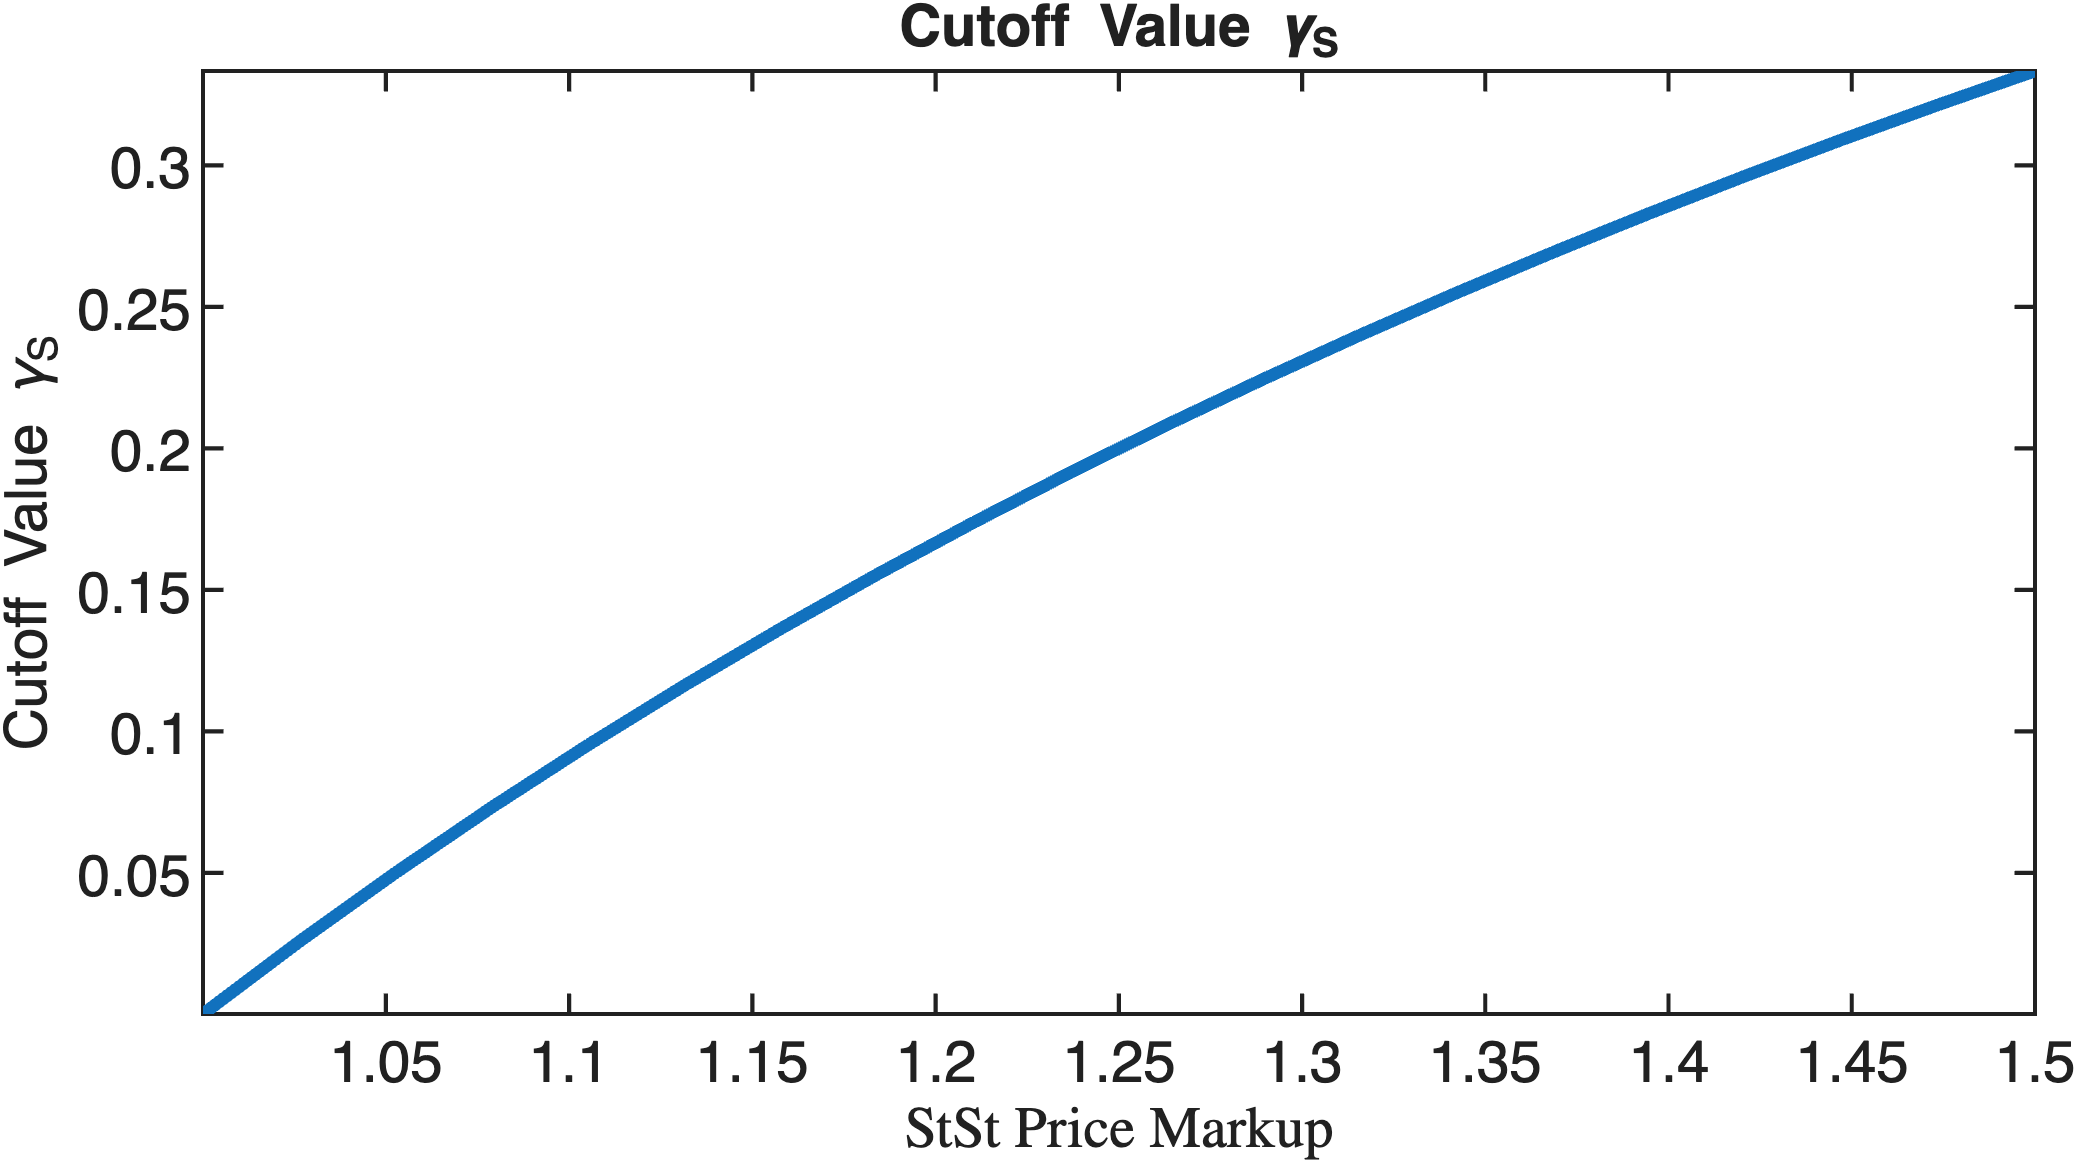
\includegraphics{fig_8_stst_gamES_cutoff.png}\\%
	{\tiny \singlespacing NOTE: The figure shows the cutoff values for $\gamma_S$ conditional on $\epsilon$. The labor demand channel of marginal costs dominates the price elasticity channel of marginal costs for values smaller than the cutoff value, vice-versa. With lower substitutability of differentiated goods (higher markups), it is more likely that the labor demand channel dominates the price elasticity channel. \par}%
\end{figure}%
% Additional Results: Steady-State of the Reduced-Form Model
%-----------------------------------------------------------
\FloatBarrier%
\subsection{Steady-State of the Reduced-Form Model}\label{sec:stst_add_gdp}%
% FIGURE STEADY STATE
\begin{figure}[h!]%
	\centering%
	\caption{Impact of $\gamma_S$ and $\psi$ (conditional on $\epsilon$) on the Steady-State}\label{fig:stst_add_gdp}%
	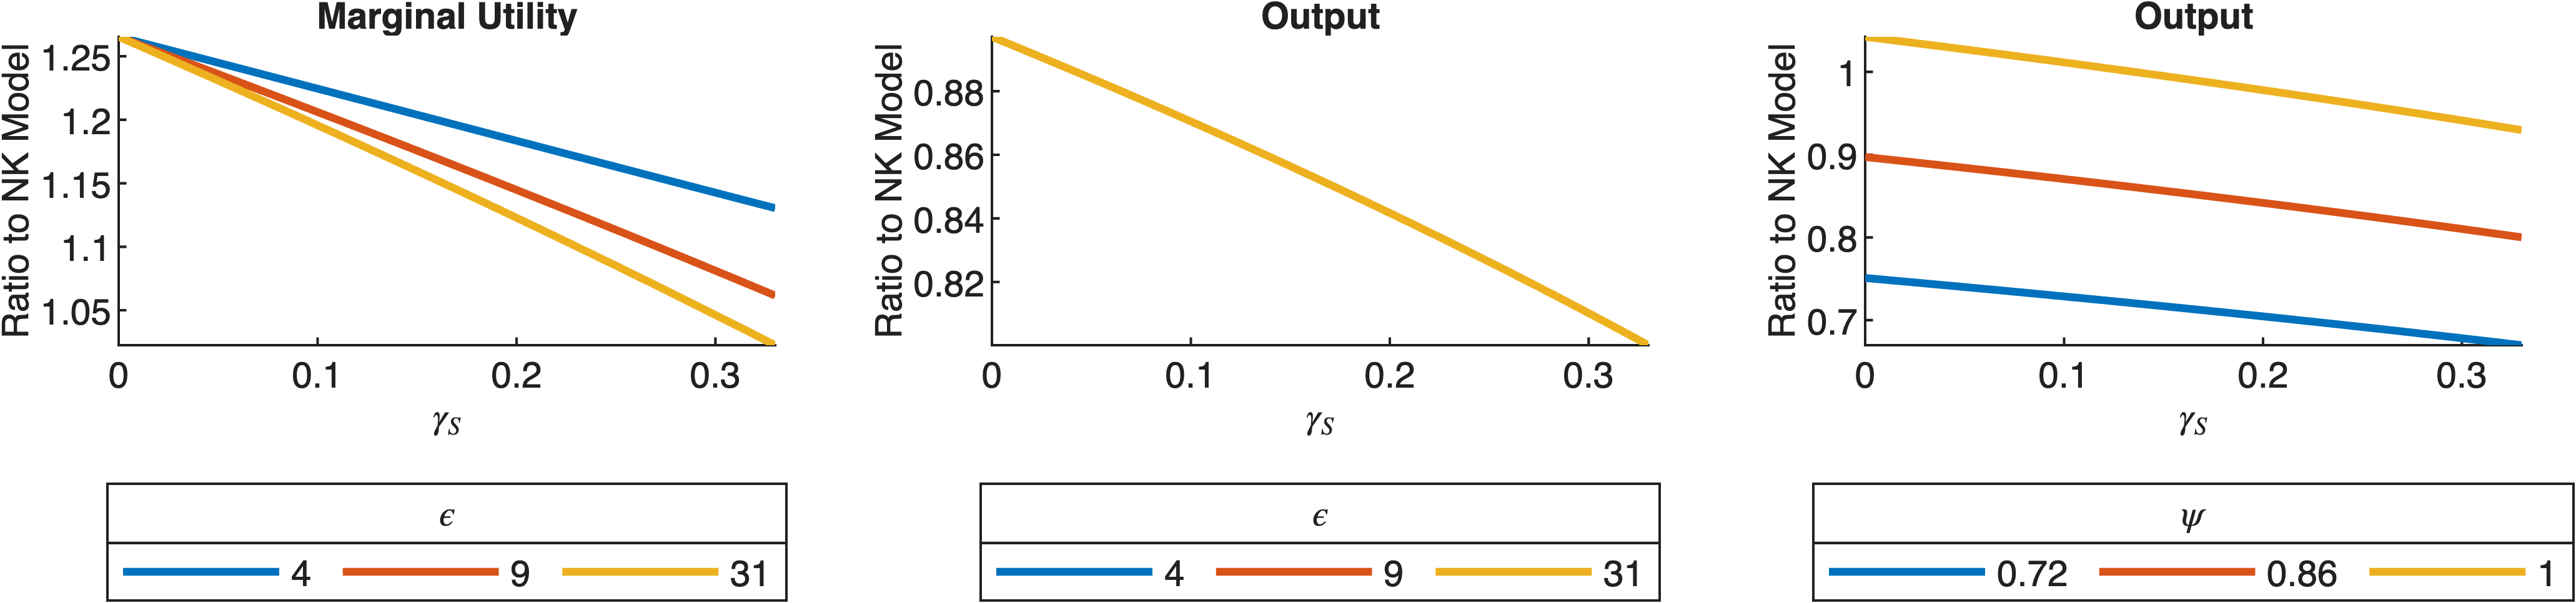
\includegraphics[width=\textwidth]{fig_9_stst_gdp.png}\\%
	{\tiny \singlespacing NOTE: The figure shows relative steady-state values of the NK-SaM model over the benchmark model for different calibrations. Search prices, $P_S$, are given as a real price level (consumption good as the numeraire) as they are zero in the benchmark model. Benchmark model and NK-SaM model are calibrated to different levels of relative home to market labor as shopping time is included in this measure for the benchmark model (see also \cref{sec:calibration}). This feature leads to a relative output steady-state not equal to one for $\gamma_S=0$.\par}%
\end{figure}%
% Additional Results: Individual Slopes
%-----------------------------------------------------------
\FloatBarrier%
\pagebreak%
\subsection{Individual Slopes of the Reduced-Form Model}\label{sec:slopes_add_individual}%
% Unemployment and Output Gap Slopes of the Reduced-Form NK-SaM Model
\begin{figure}[h!]%
    \centering%
    \caption{Unemployment and Output Gap Slopes of the Reduced-Form NK-SaM Model}\label{fig:slopes_add_individual}%
    \begin{subfigure}{\textwidth}%
        \centering%
        \caption{Variation of the Slopes of the Goods Market Channels}\label{fig:app_slopes_tot_caput}%
        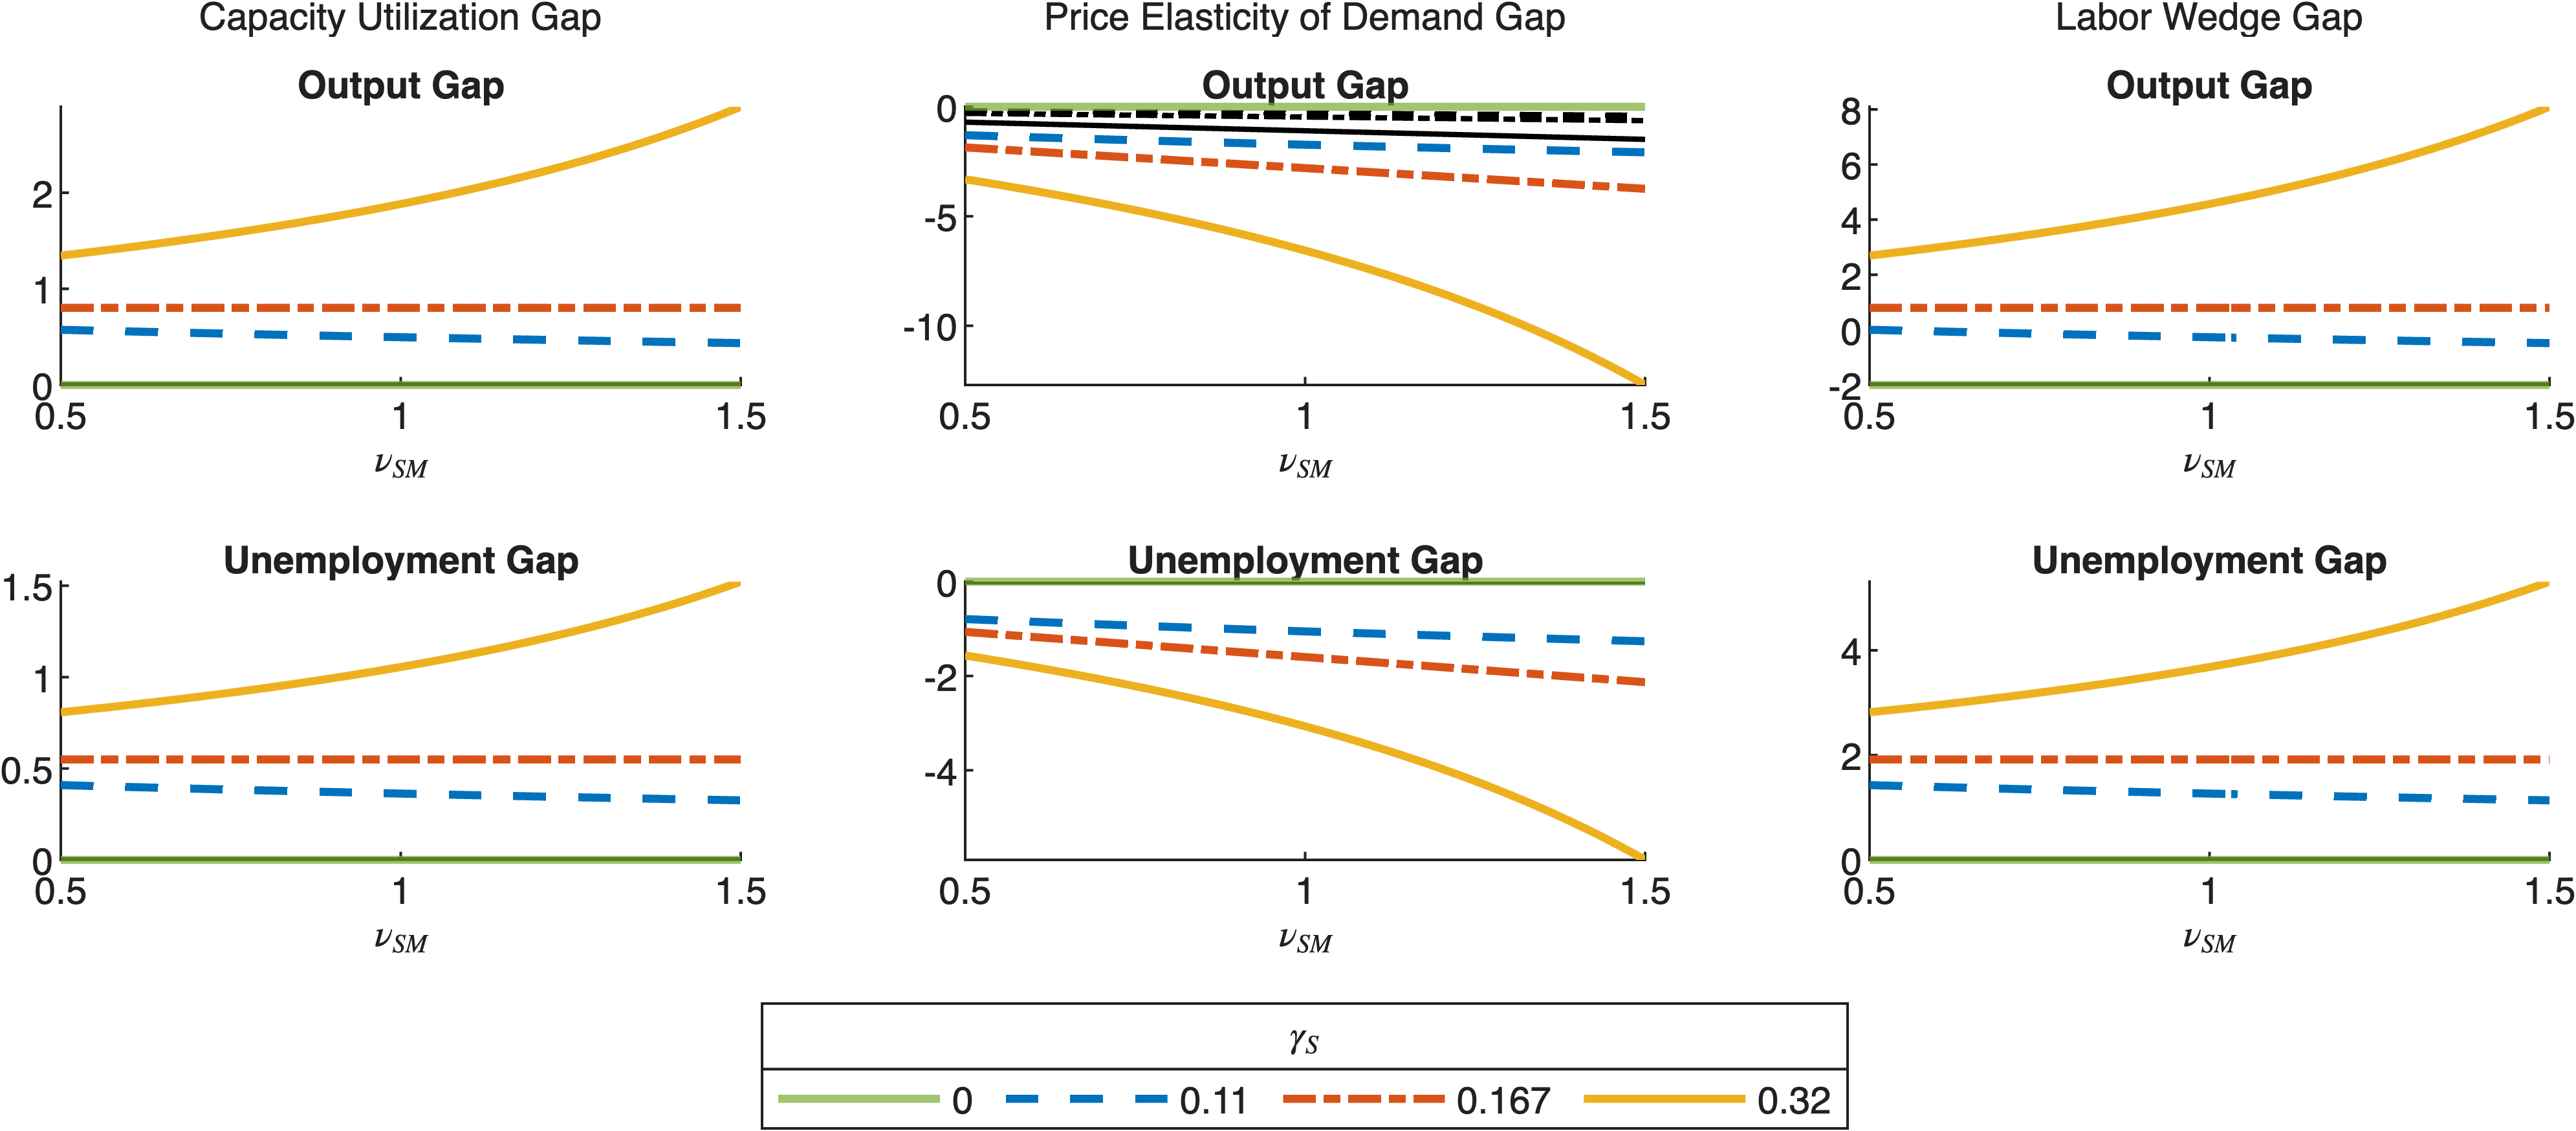
\includegraphics[width=\textwidth]{fig_10_slopes_5eq_ps_cu.png}%
    \end{subfigure}\\%
	\vspace{0.2in}%
    \begin{subfigure}{\textwidth}%
        \centering%
        \caption{Variation of the Slopes of the 5-Equation Model Dynamic Equations}\label{fig:app_slopes_tot_asad}%
        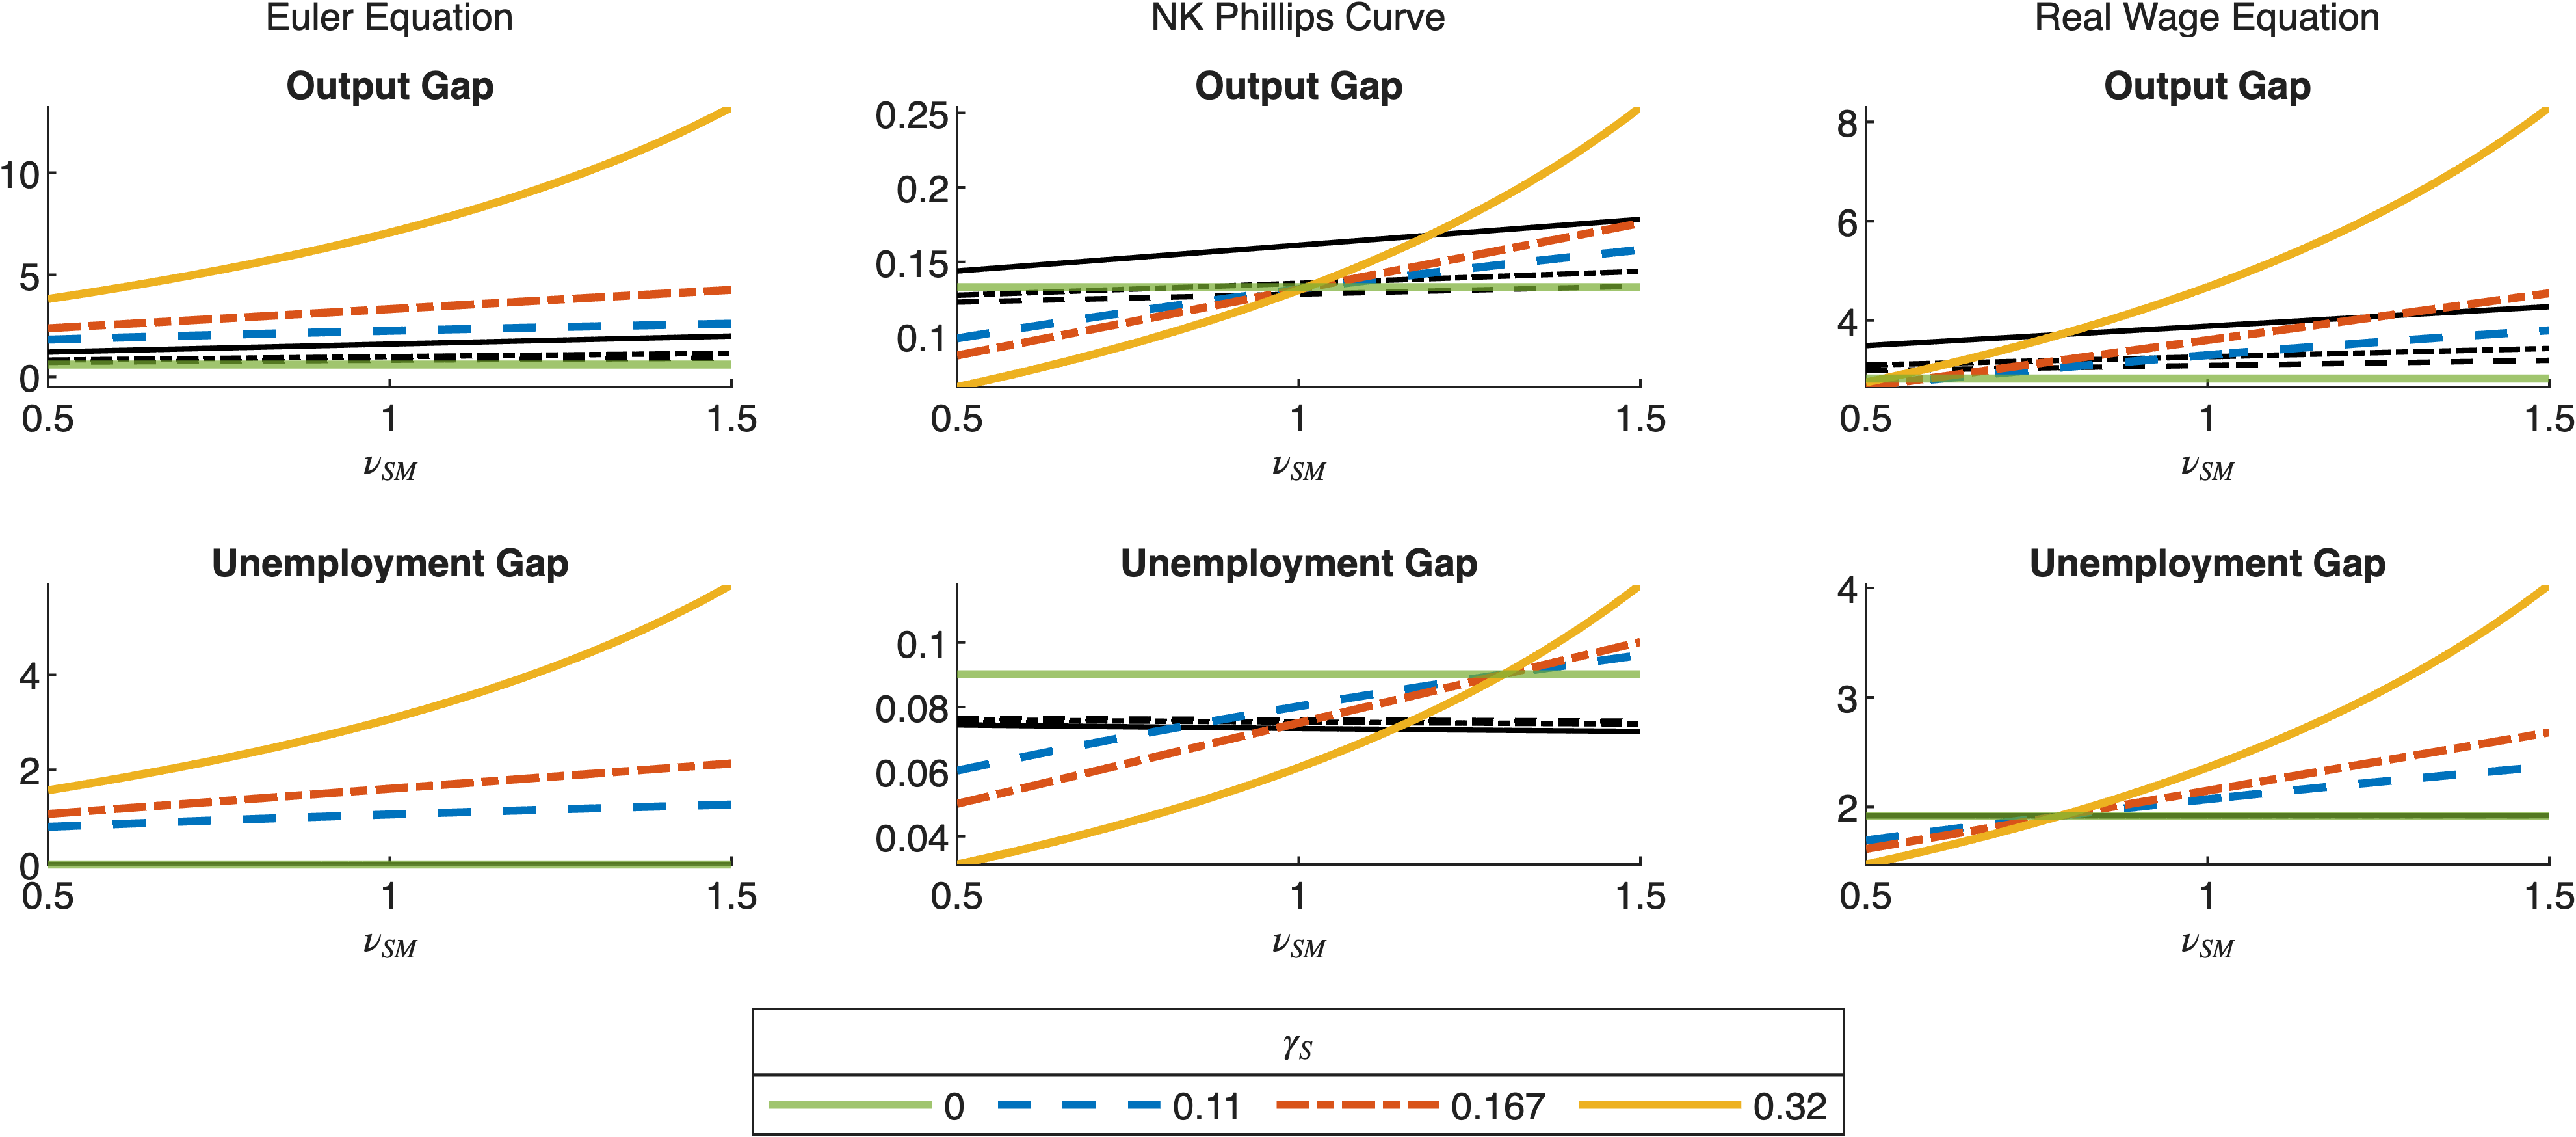
\includegraphics[width=\textwidth]{fig_11_slopes_5eq_asad.png}%
    \end{subfigure}\\%
    {\tiny \singlespacing NOTE: The graphs show the impact of varying $\nu_S$ with a fixed $\nu_M$ on the slopes of the goods market SaM channels and the reduced-form NK-SaM model (inclduing home production). The benchmark model is shown by the full horizontal line ($\gamma_S=0$). The NK-SaM model is shown in two variants for three different values of $\gamma_S$ indicated by the dashed, dashed-dotted, and full lines. First, the bold-colored lines show $\Gamma_S \approx 0$. Second, the thin-black lines show $\Gamma_S=-\infty$ implying an substitution elasticity of $\approx 0$ for the matching inputs.\par}%
\end{figure}%
% FIGURE: IRFs (Decomposition) to Further Cost-Push Shocks
%-----------------------------------------------------------
\FloatBarrier%
\pagebreak%
\subsection{Results of Further Cost-Push Shocks}\label{sec:irf_add_cost-push}%
% FIGURES
\begin{figure}[h!]%
    \centering%
    \caption{Channel Decomposition - IRFs of Further Cost-Push Shocks}\label{fig:irf_add_cost-push}%
    \begin{subfigure}{\textwidth}%
        \centering%
        \caption{IRFs to an Expansionary Matching Efficiency Shock}%
        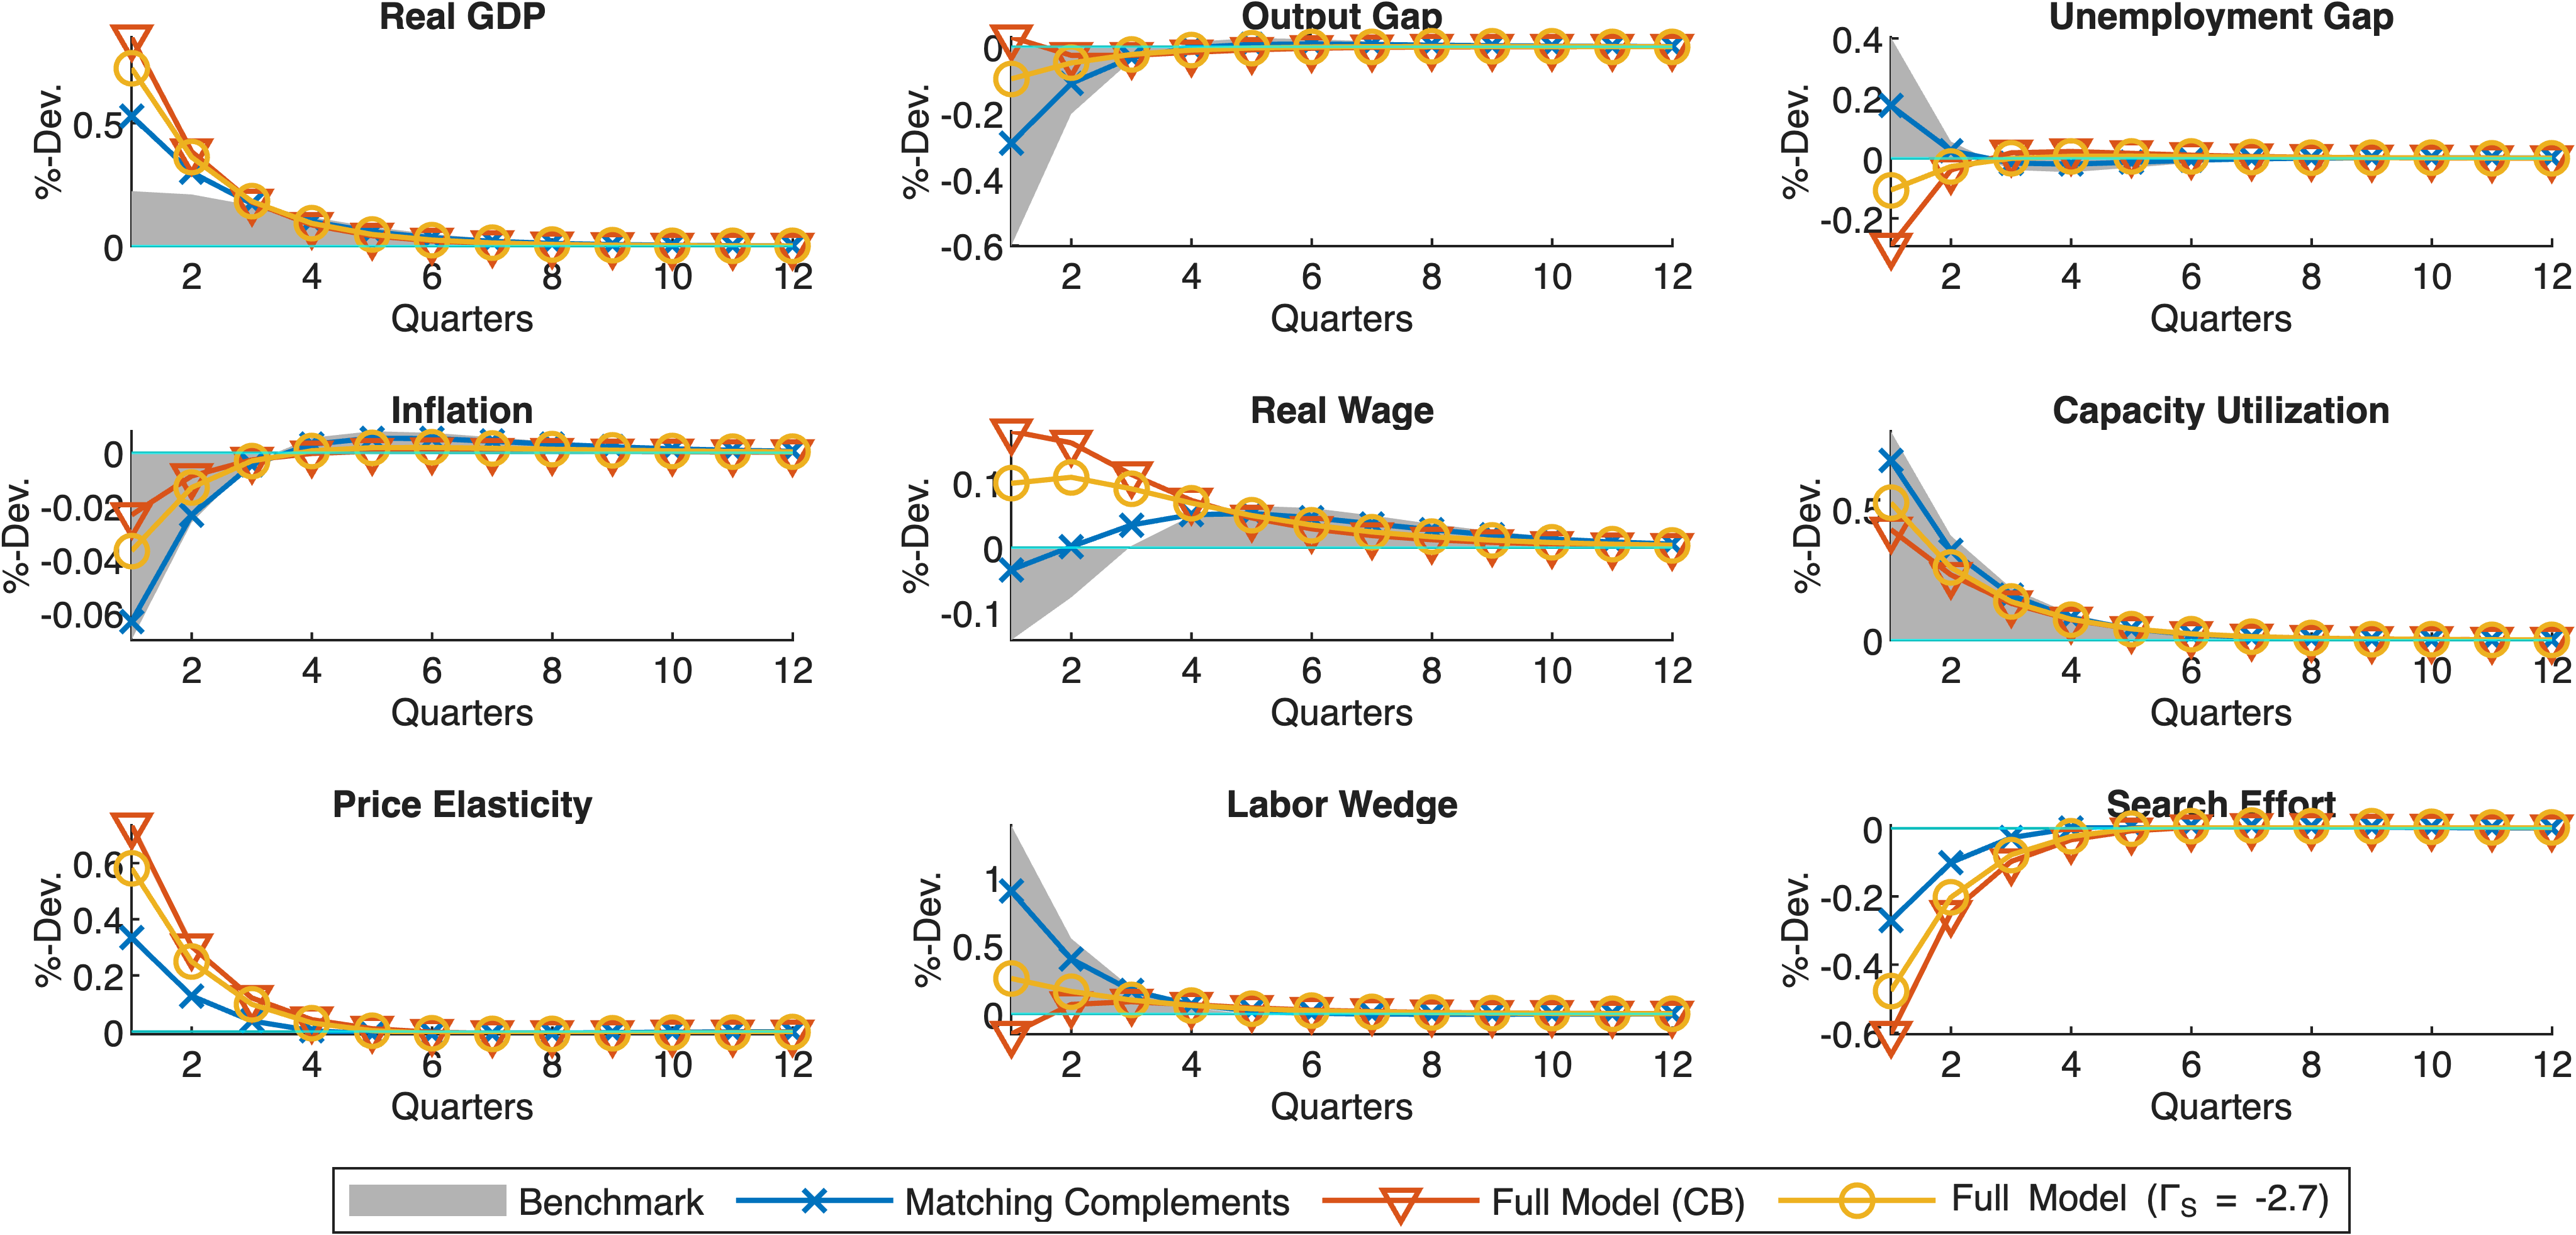
\includegraphics[width=\textwidth]{fig_12_irf_default_efficiency.png}%
    \end{subfigure}\\%
	\vspace{0.2in}%
    \begin{subfigure}{\textwidth}%
        \centering%
        \caption{IRFs to an Expansionary EIS Shock}%
        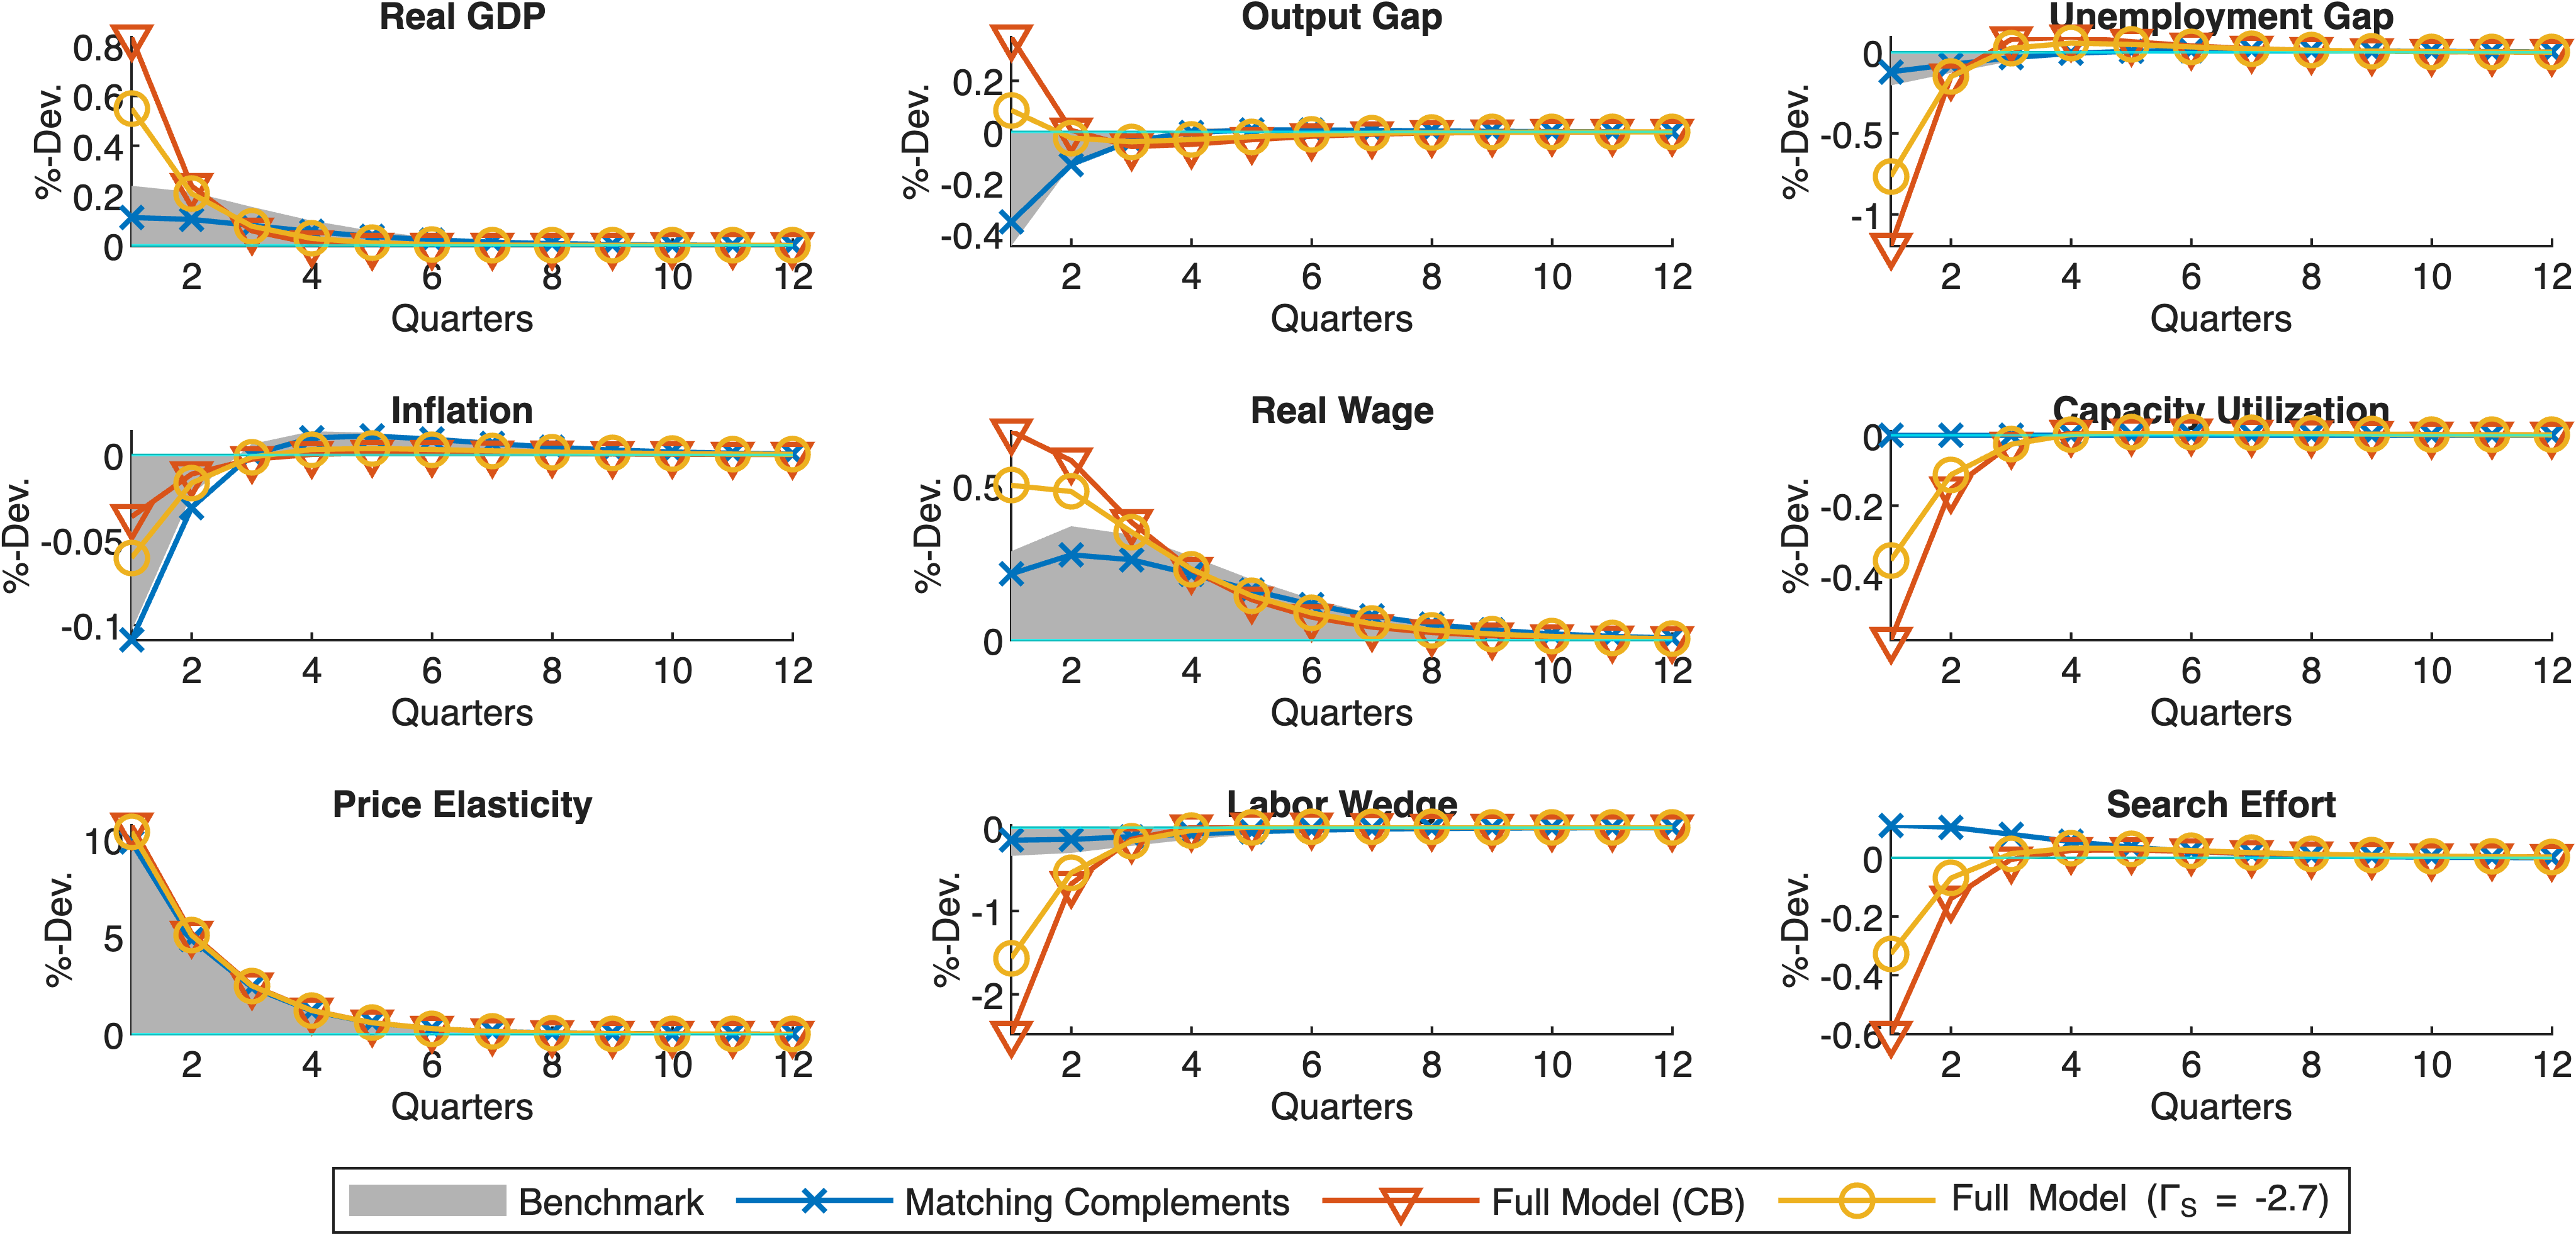
\includegraphics[width=\textwidth]{fig_13_irf_default_eis.png}%
    \end{subfigure}\\%
    {\tiny \singlespacing NOTE: The figure shows IRFs to a one standard deviation (a) expansionary matching efficiency and (b) expansionary elasticity of substitution (EIS) shock using the model presented in \cref{sec:model} and \cref{sec:dynamics}. The benchmark model follows \cref{prop:nosam}, the ''matching complements'' model sets $\Gamma_S = -\infty$, the CES model sets $\Gamma_S = -2.7$, the Cobb-Douglas model is calibrated as in \cref{tab:calibration}.\par}%
\end{figure}%
% ROBUSTNESS: Alternative Calibration
%-----------------------------------------------------------
\FloatBarrier%
\pagebreak%
\subsection{Alternative Calibration of the Model}\label{sec:calibration_add}%
% IRF Figures - TFP and Demand Shocks
\begin{figure}[h!]%
    \centering%
    \caption{Variation in $\nicefrac{\nu_S}{\nu_M}$ - IRFs to Expansionary TFP and Demand Shocks}%
    \begin{subfigure}{\textwidth}%
        \centering%
        \caption{IRFs to an Expansionary TFP Shock}%
        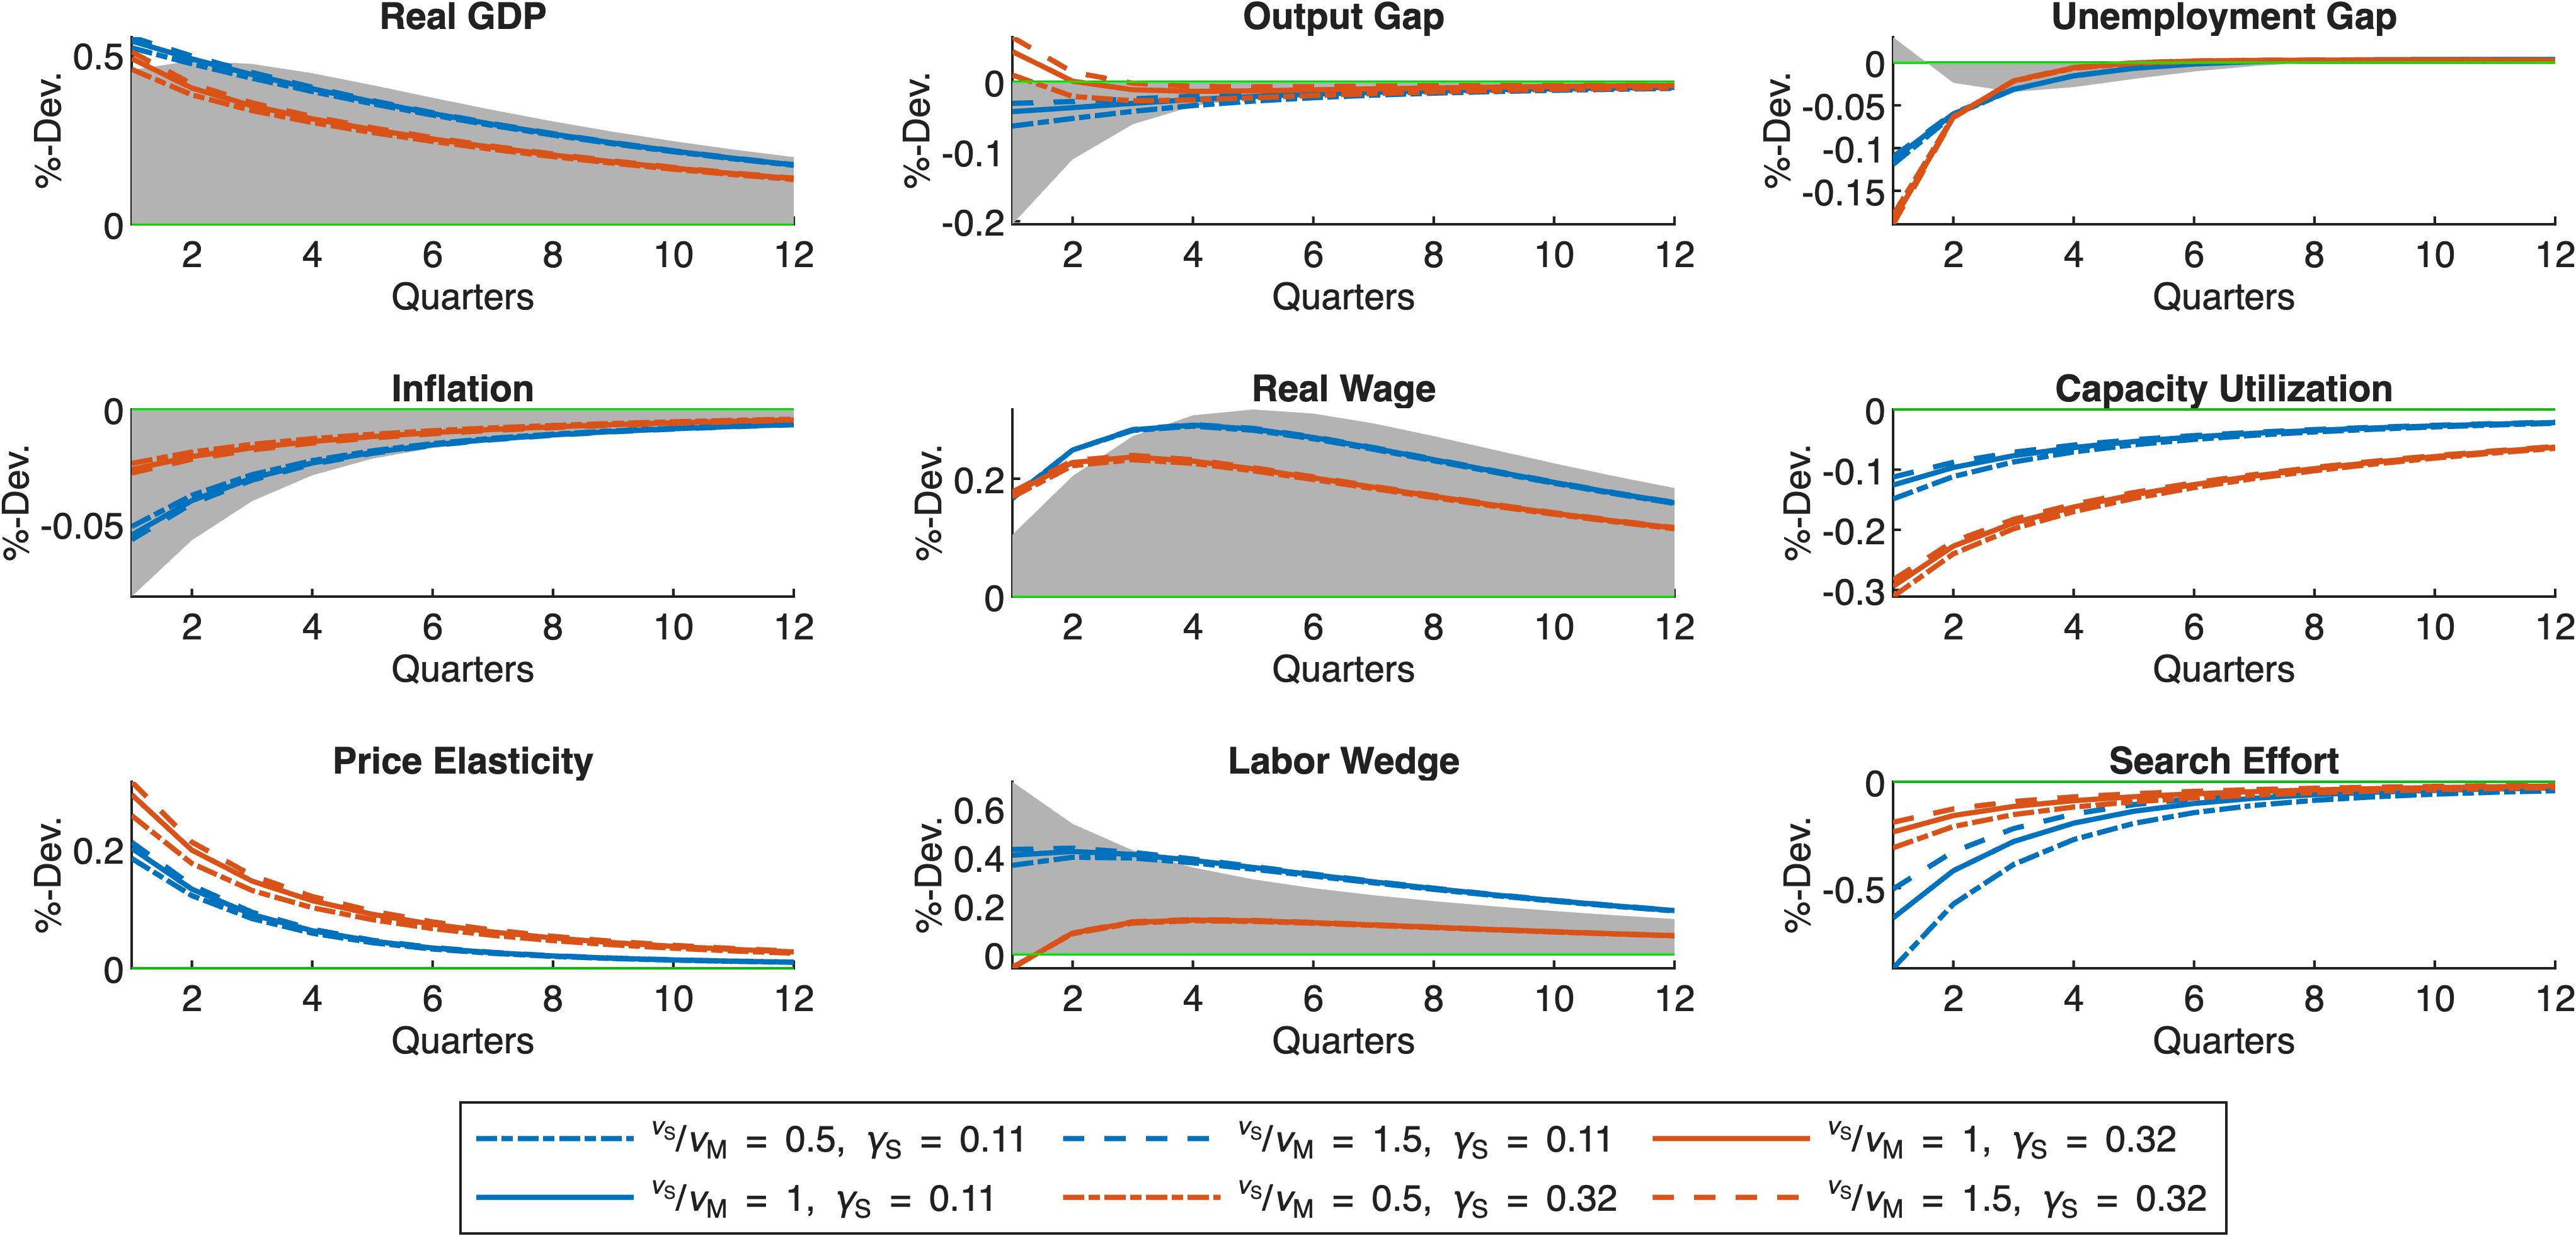
\includegraphics[width=\textwidth]{fig_14_irf_robust_nuSnuM_tfp.png}%
    \end{subfigure}\\%
	\vspace{0.2in}%
    \begin{subfigure}{\textwidth}%
        \centering%
        \caption{IRFs to an Expansionary Monetary Policy Shock}%
        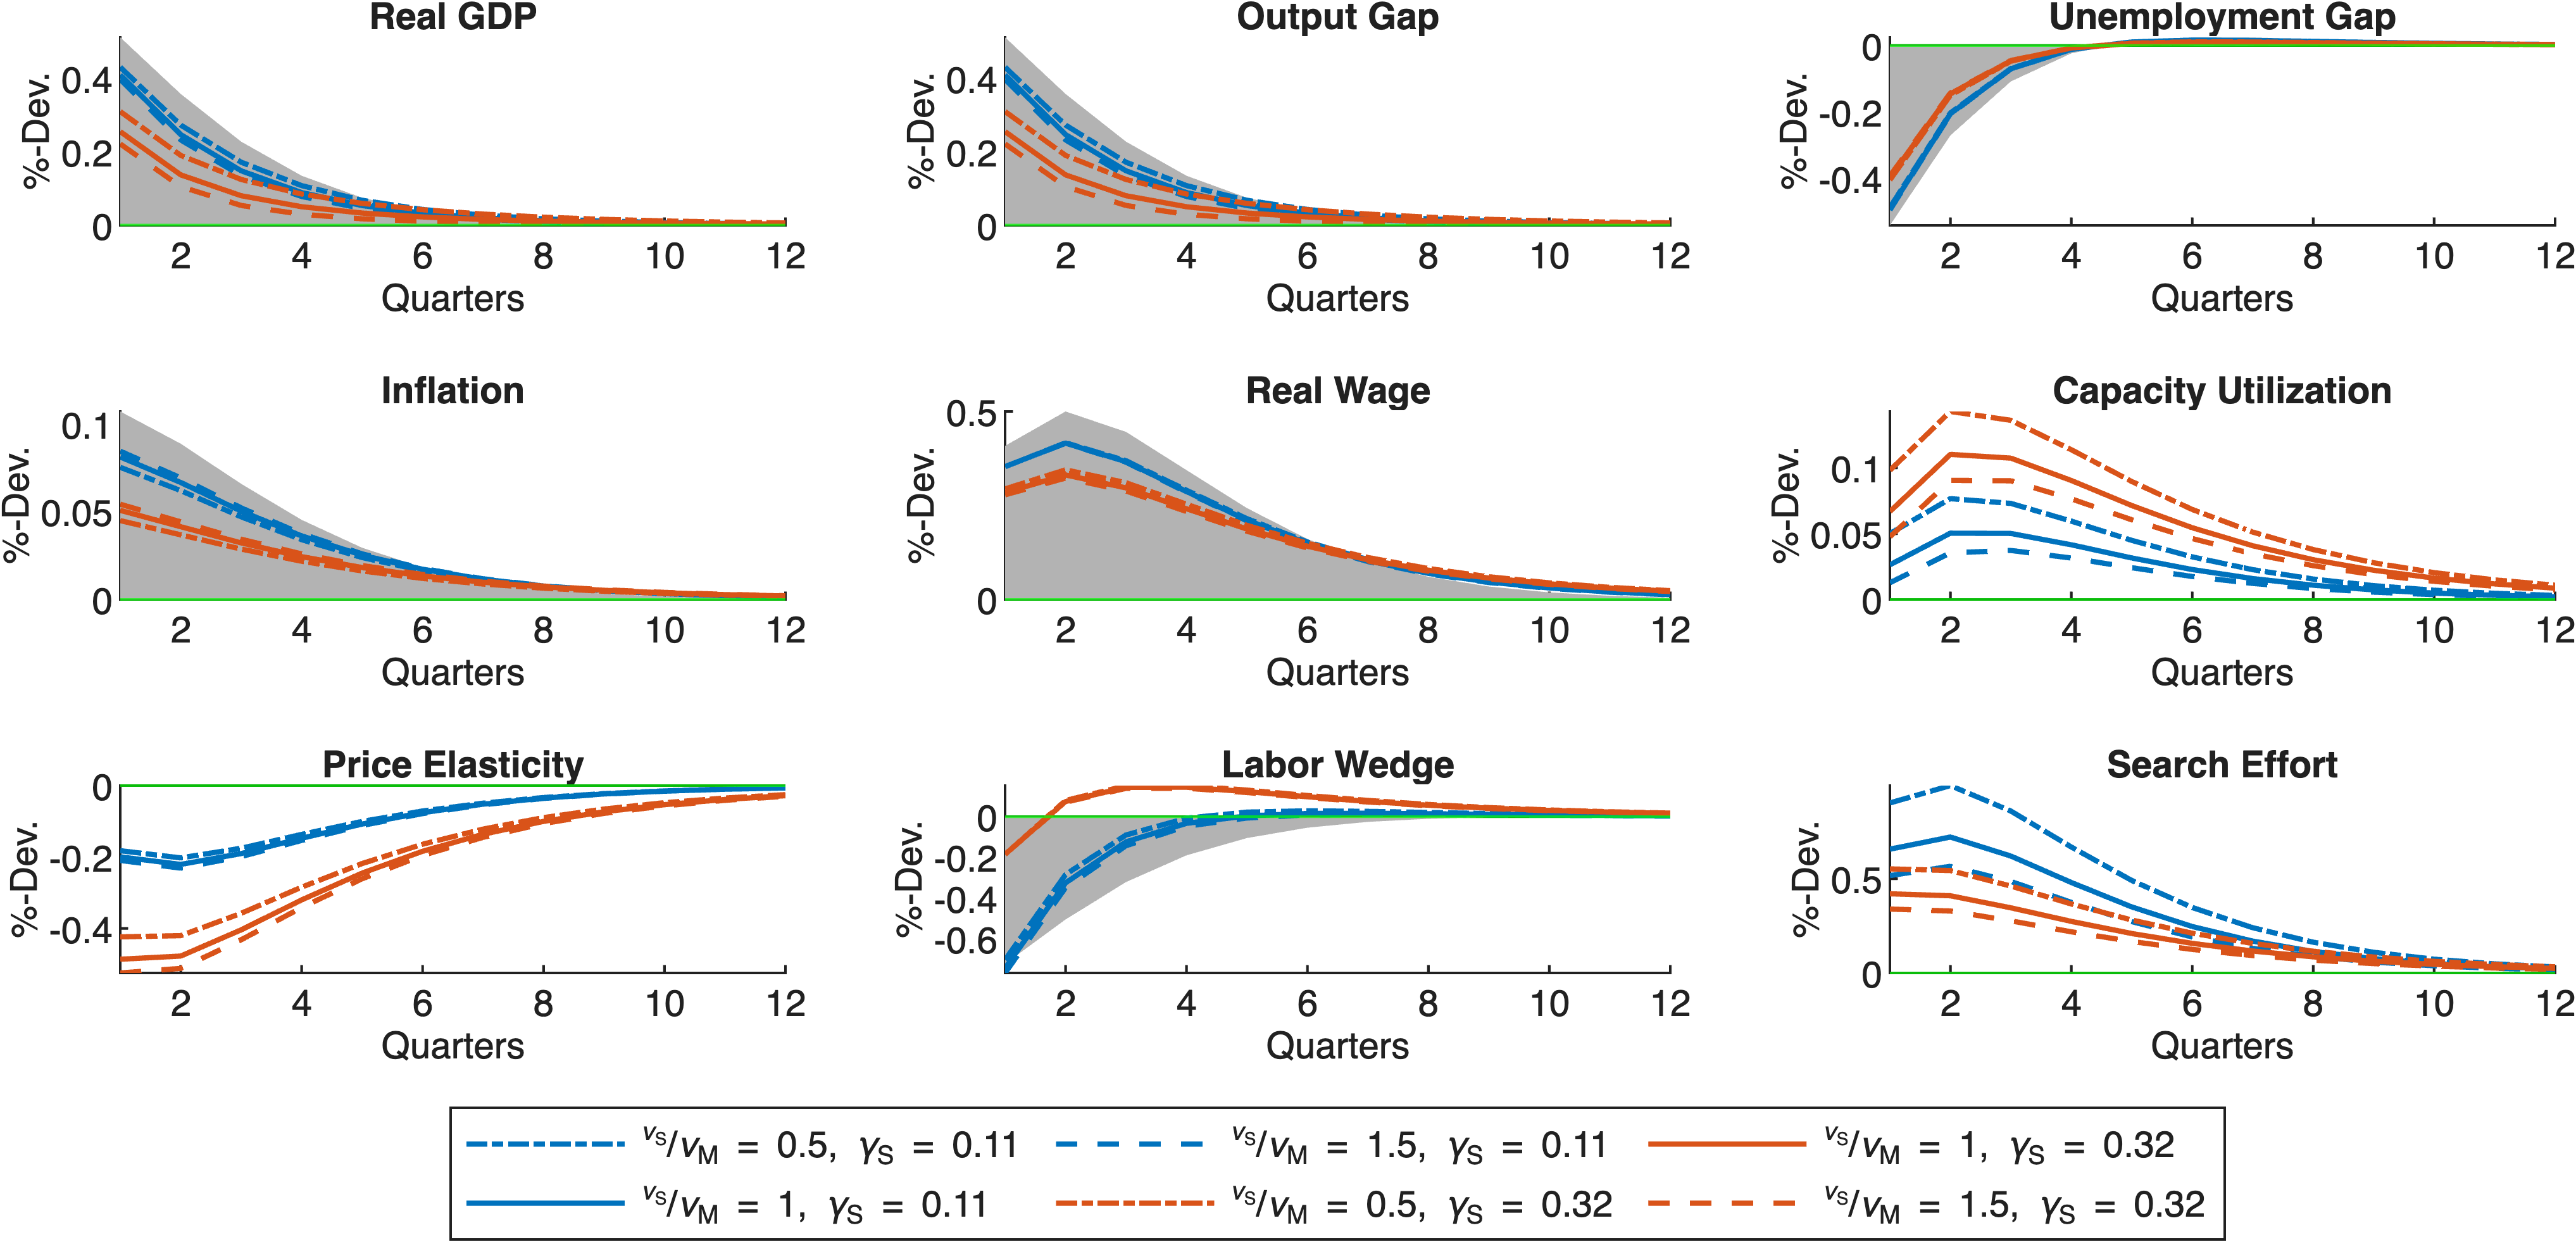
\includegraphics[width=\textwidth]{fig_15_irf_robust_nuSnuM_policy.png}%
    \end{subfigure}\\%
    {\tiny \singlespacing NOTE: The figure shows IRFs to one standard deviation expansionary shocks using the model presented in \cref{sec:model} and \cref{sec:dynamics}. The benchmark model (grey areas)follows \cref{prop:nosam}, the NK-SaM model is calibrated as given in the legend with varying values for $\gamma_S$ and $\nicefrac{\nu_S}{\nu_M}$.\par}%
\end{figure}%
% IRF Figures - Cost Push Shocks
\begin{figure}[h!]%
	\centering%
	\caption{Variation in $\nicefrac{\nu_S}{\nu_M}$ - IRFs to Expansionary Cost Push Shocks}
	\begin{subfigure}{\textwidth}%
		\centering%
        \caption{IRFs to an Expansionary EIS Shock}%
        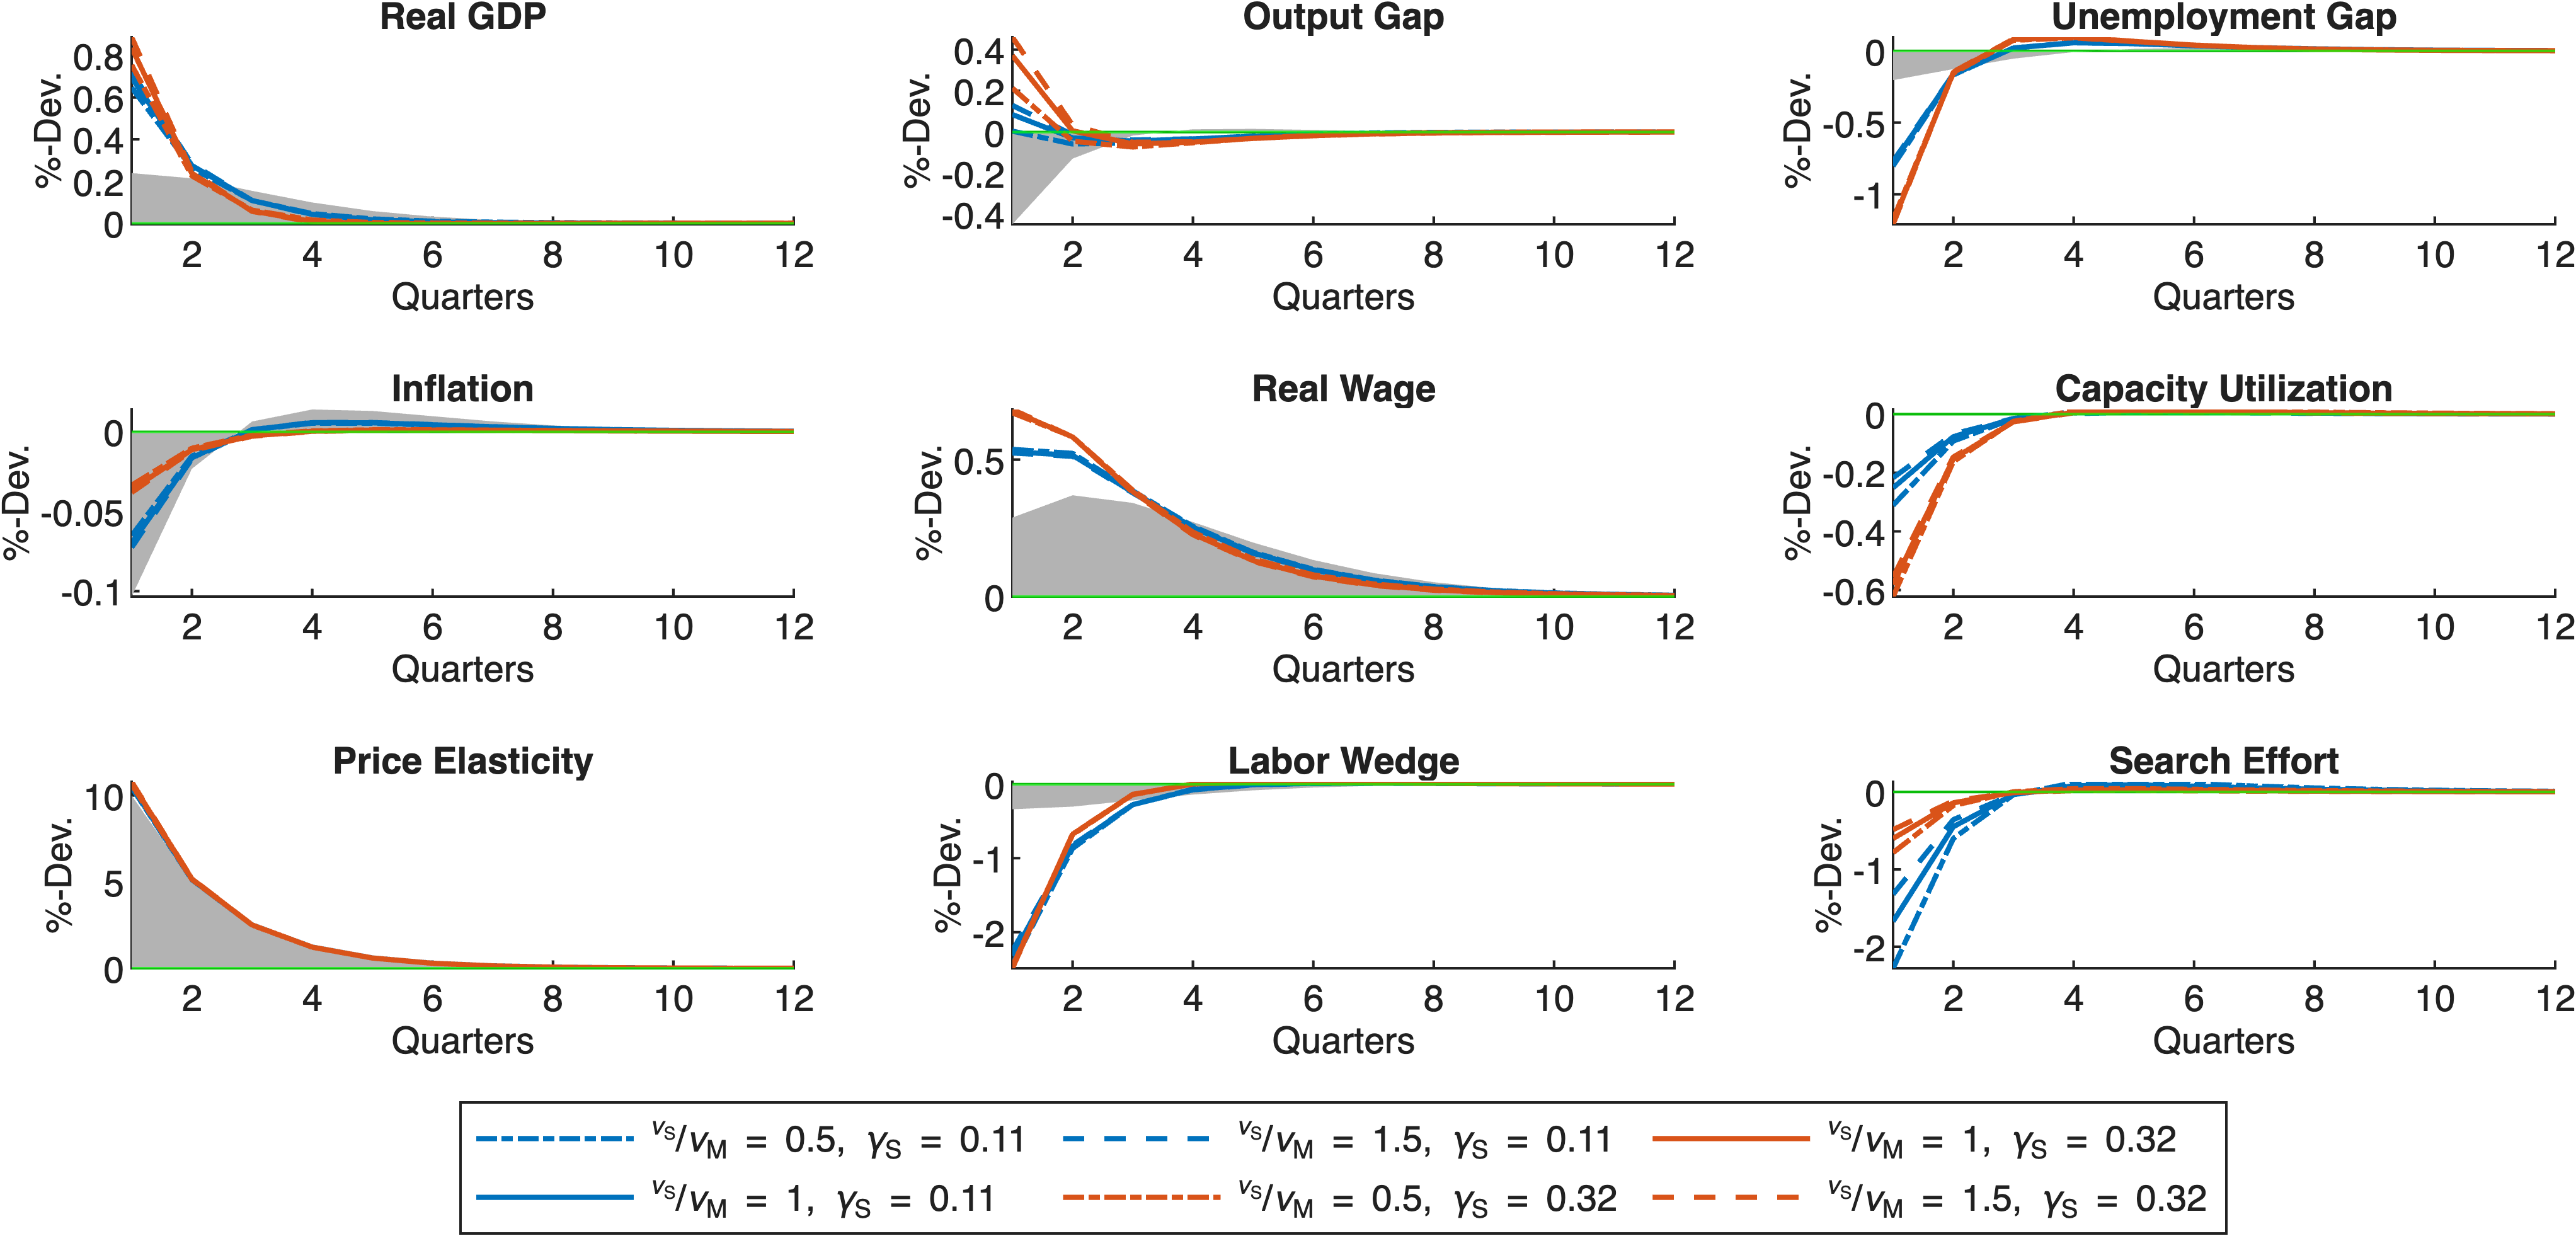
\includegraphics[width=\textwidth]{fig_16_irf_robust_nuSnuM_eis.png}%
	\end{subfigure}\\%
	\vspace{0.2in}%
	\begin{subfigure}{\textwidth}%
        \centering%
        \caption{IRFs to an Expansionary Search Effort Shock}%
        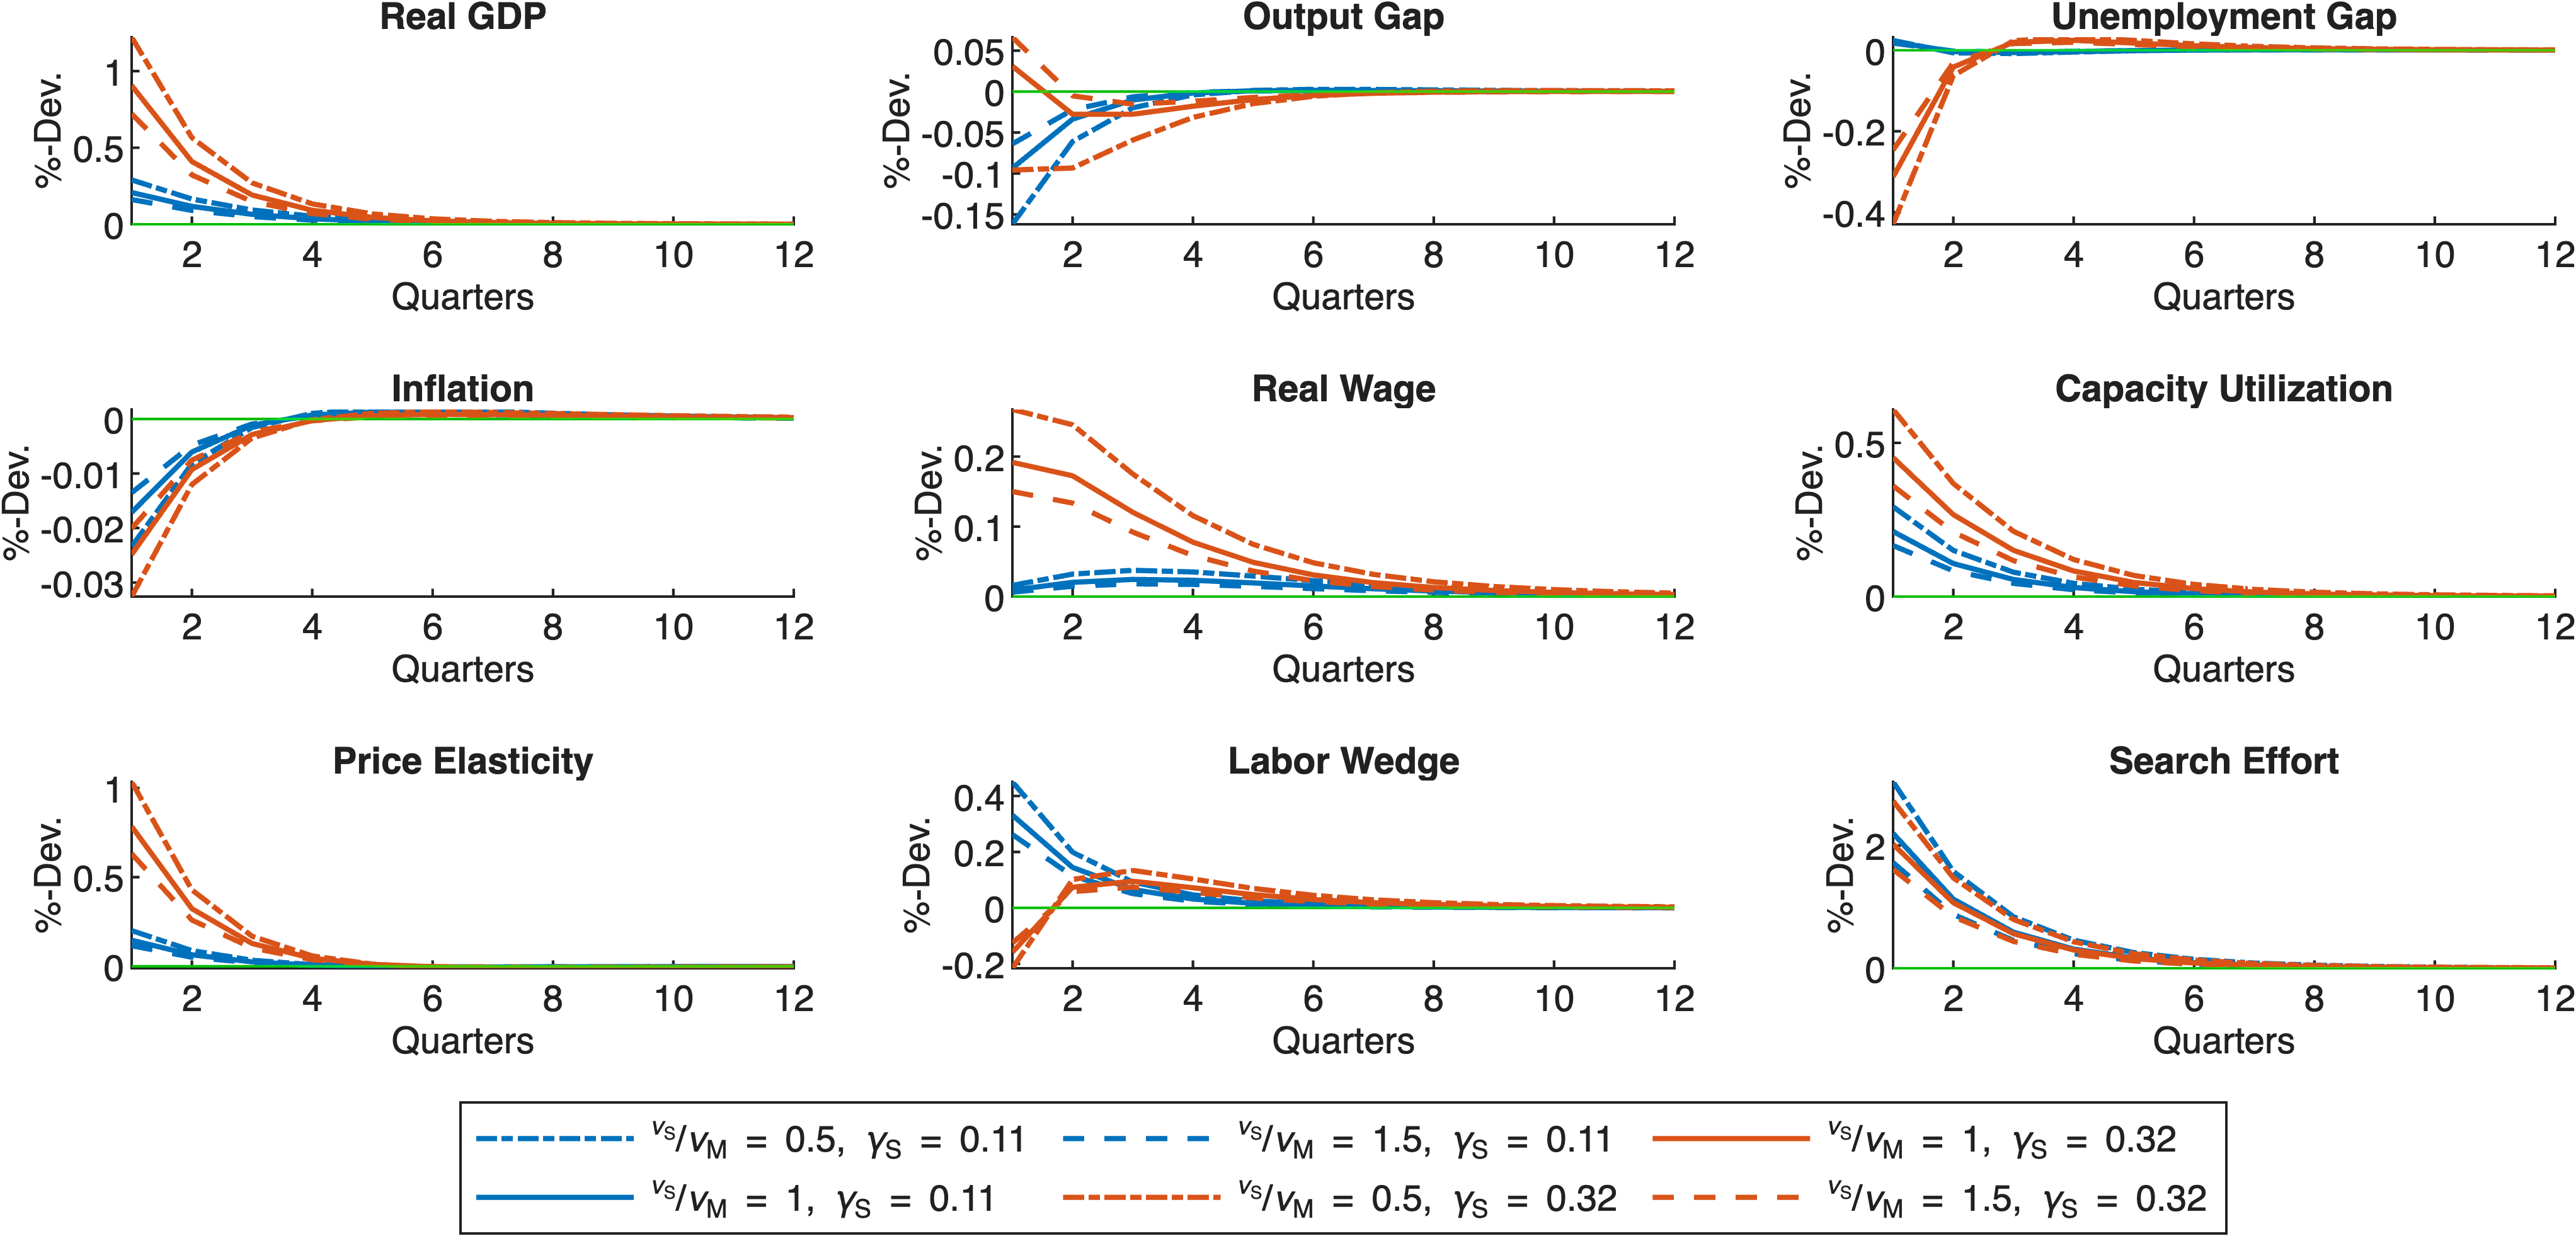
\includegraphics[width=\textwidth]{fig_17_irf_robust_nuSnuM_search.png}%
    \end{subfigure}\\%
    {\tiny \singlespacing NOTE: The figure shows IRFs to one standard deviation expansionary shocks using the model presented in \cref{sec:model} and \cref{sec:dynamics}. The benchmark model (grey areas)follows \cref{prop:nosam}, the NK-SaM model is calibrated as given in the legend with varying values for $\gamma_S$ and $\nicefrac{\nu_S}{\nu_M}$.\par}%
\end{figure}%
% Statistics Table - ALTERNATIVE CALIBRATION
%-----------------------------------------------------------
\pagebreak%
\begin{table}[h!]%
	\begin{center}%
		\begin{footnotesize}%
			\caption{Alternative Calibration - Relative Standard Deviations and Correlations}\label{tab:simul_stats_app}%
			\begin{tabular}{l r r r r r r r r}%
				\hline%
				$\boldsymbol{\gamma_S = 0.11}$ & \multicolumn{2}{c}{TFP} & \multicolumn{2}{c}{Policy} & \multicolumn{2}{c}{Cost-Push} & \multicolumn{2}{c}{Search}\\%
				Variable & Rel.Std. & Corr. & Rel.Std. & Corr. & Rel.Std. & Corr. & Rel.Std. & Corr.\\%
				\hline \hline%
				Output Gap & 0.07 & -0.98 & 1.00 & 1.00 & 0.15 & 0.64 & 0.42 & -0.96\\%
				UE Gap & 0.16 & -0.73 & 1.12 & -0.96 & 1.11 & -0.97 & 0.10 & 0.63\\%
				Inflation & 0.08 & -0.94 & 0.23 & 0.96 & 0.10 & -0.97 & 0.08 & -0.94\\%
				Real Wage & 0.60& 0.89 & 1.36 & 0.84 & 1.07 & 0.82 & 0.17 & 0.47\\%
				Utilization & 0.20 & -0.97 & 0.17 & 0.67 & 0.36 & -0.99 & 0.99 & 1.00\\%
				Marginal Cost & 0.48 & -0.87 & 1.17 & 0.87 & 1.40 & 0.92 & 1.10 & -0.98\\%
				Price Elasticity & 0.30 & 0.87 & 0.72 & -0.87 & 15.69 & 0.99 & 0.68 & 0.98\\%
				Labor Wedge & 0.88 & 0.99 & 1.71 & -0.97 & 3.33 & -1.00 & 1.51 & 0.99\\%
				Search Effort & 0.94 & -0.87 & 2.36 & 0.87 & 2.39 & -0.98 & 10.35 & 1.00\\%
				\hline%
				\hline%
				$\boldsymbol{\Gamma_S = -2.7}$ & \multicolumn{2}{c}{TFP} & \multicolumn{2}{c}{Policy} & \multicolumn{2}{c}{Cost-Push} & \multicolumn{2}{c}{Search}\\%
				Variable & Rel.Std. & Corr. & Rel.Std. & Corr. & Rel.Std. & Corr. & Rel.Std. & Corr.\\%
				\hline \hline%
				Output Gap & 0.10 & -0.98 & 1.00 & 1.00 & 0.18 & 0.69 & 0.20 & 0.95\\%
				UE Gap & 0.14 & -0.73 & 1.41 & -0.95 & 1.38 & -0.97 & 0.52 & -0.94\\%
				Inflation & 0.11 & -0.96 & 0.31 & 0.96 & 0.11 & -0.98 & 0.01 & -0.30\\%
				Real Wage & 0.59 & 0.87 & 1.83 & 0.84 & 1.27 & 0.82 & 0.40 & 0.90\\%
				Utilization & 0.39 & -0.98 & 0.36 & 0.72 & 0.64 & -1.00 & 0.28 & 0.97\\%
				Marginal Cost & 0.66 & -0.94 & 1.42 & 0.87 & 1.90 & 0.94 & 0.11 & 0.40\\%
				Price Elasticity & 0.23 & -0.13 & 2.03 & -0.94 & 19.66 & 0.99 & 0.95 & 1.00\\%
				Labor Wedge & 0.93 & 0.99 & 0.94 & -0.79 & 2.84 & -1.00 & 0.72 & -0.98\\%
				Search Effort & 0.20 & 0.25 & 1.75 & 0.94 & 0.60 & -0.96 & 1.69 & 1.00\\%
				\hline%
				\hline%
				$\boldsymbol{\frac{\nu_S}{\nu_M} = 0.5}$ & \multicolumn{2}{c}{TFP} & \multicolumn{2}{c}{Policy} & \multicolumn{2}{c}{Cost-Push} & \multicolumn{2}{c}{Search}\\%
				Variable & Rel.Std. & Corr. & Rel.Std. & Corr. & Rel.Std. & Corr. & Rel.Std. & Corr.\\%
				\hline \hline%
				Output Gap & 0.07 & -0.51 & 1.00 & 1.00 & 0.32 & 0.82 & 0.10 & -0.90\\%
				UE Gap & 0.30 & -0.69 & 1.19 & -0.92 & 1.56 & -0.98 & 0.34 & -0.92\\%
				Inflation & 0.05 & -0.99 & 0.17 & 0.97 & 0.05 & -1.00 & 0.03 & -0.99\\%
				Real Wage & 0.60 & 0.92 & 1.50 & 0.86 & 1.17 & 0.82 & 0.28 & 0.89\\%
				Utilization & 0.63 & -0.99 & 0.62 & 0.78 & 0.83 & -1.00 & 0.53 & 0.99\\%
				Marginal Cost & 0.21 & -0.95 & 0.79 & 0.92 & 2.01 & 0.95 & 0.36 & -1.00\\%
				Price Elasticity & 0.49 & 0.95 & 1.85 & -0.92 & 14.89 & 0.98 & 0.80 & 1.00\\%
				Labor Wedge & 0.38 & 0.44 & 0.92 & -0.22 & 3.27 & -1.00 & 0.23 & -0.50\\%
				Search Effort & 0.59 & -0.94 & 2.40 & 0.92 & 1.05 & -0.99 & 2.31 & 1.00\\%
				\hline%
				\hline%
				$\boldsymbol{\frac{\nu_S}{\nu_M} = 1.5}$ & \multicolumn{2}{c}{TFP} & \multicolumn{2}{c}{Policy} & \multicolumn{2}{c}{Cost-Push} & \multicolumn{2}{c}{Search}\\%
				Variable & Rel.Std. & Corr. & Rel.Std. & Corr. & Rel.Std. & Corr. & Rel.Std. & Corr.\\%
				\hline \hline%
				Output Gap & 0.10 & 0.55 & 1.00 & 1.00 & 0.52 & 0.97 & 0.09 & 0.79\\%
				UE Gap & 0.29 & -0.70 & 1.73 & -0.98 & 1.37 & -0.98 & 0.33 & -0.92\\%
				Inflation & 0.05 & -0.99 & 0.31 & 0.90 & 0.04 & -1.00 & 0.03 & -0.99\\%
				Real Wage & 0.57 & 0.91 & 2.10 & 0.74 & 1.00 & 0.82 & 0.27 & 0.90\\%
				Utilization & 0.53 & -1.00 & 0.59 & 0.54 & 0.63 & -1.00 & 0.53 & 0.99\\%
				Marginal Cost & 0.23 & -0.95 & 1.44 & 0.82 & 1.65 & 0.94 & 0.37 & -1.00\\%
				Price Elasticity & 0.54 & 0.95 & 3.39 & -0.82 & 12.85 & 0.97 & 0.87 & 1.00\\%
				Labor Wedge & 0.37 & 0.40 & 1.31 & -0.45 & 2.81 & -1.00 & 0.23 & -0.52\\%
				Search Effort & 0.33 & -0.95 & 2.18 & 0.82 & 0.55 & -1.00 & 2.30 & 1.00\\%
				\hline%
			\end{tabular}\\%
			\vspace{0.1in}%
			{\tiny NOTE: The table shows simulated second moments for the NK-SaM model. It shows relative standard deviations - standard deviation of each variable relative to standard deviation of real GDP - and correlations of each variable with real GDP. We consider each shock separately in the simulation.\par}%
		\end{footnotesize}%
	\end{center}%
\end{table}%
%--------------------------------------------------------------------------
% E. APPENDIX
%--------------------------------------------------------------------------
%-----------------------------------------------------------
% Appendix - Results of the Robustness Analysis
%-----------------------------------------------------------
\clearpage%
\FloatBarrier%
\section{Results of the Robustness Analysis}\label{sec:robust}%
% ROBUSTNESS: Dropping Home Production
%-----------------------------------------------------------
\subsection{Robustness - Dropping Home Production}\label{sec:robust_hw}%
% Slope Figures
\begin{figure}[h!]%
    \centering%
    \caption{Relative Slopes - Including Home Production relative to excluding Home Production}\label{fig:app_slopes_robust_hw}%
    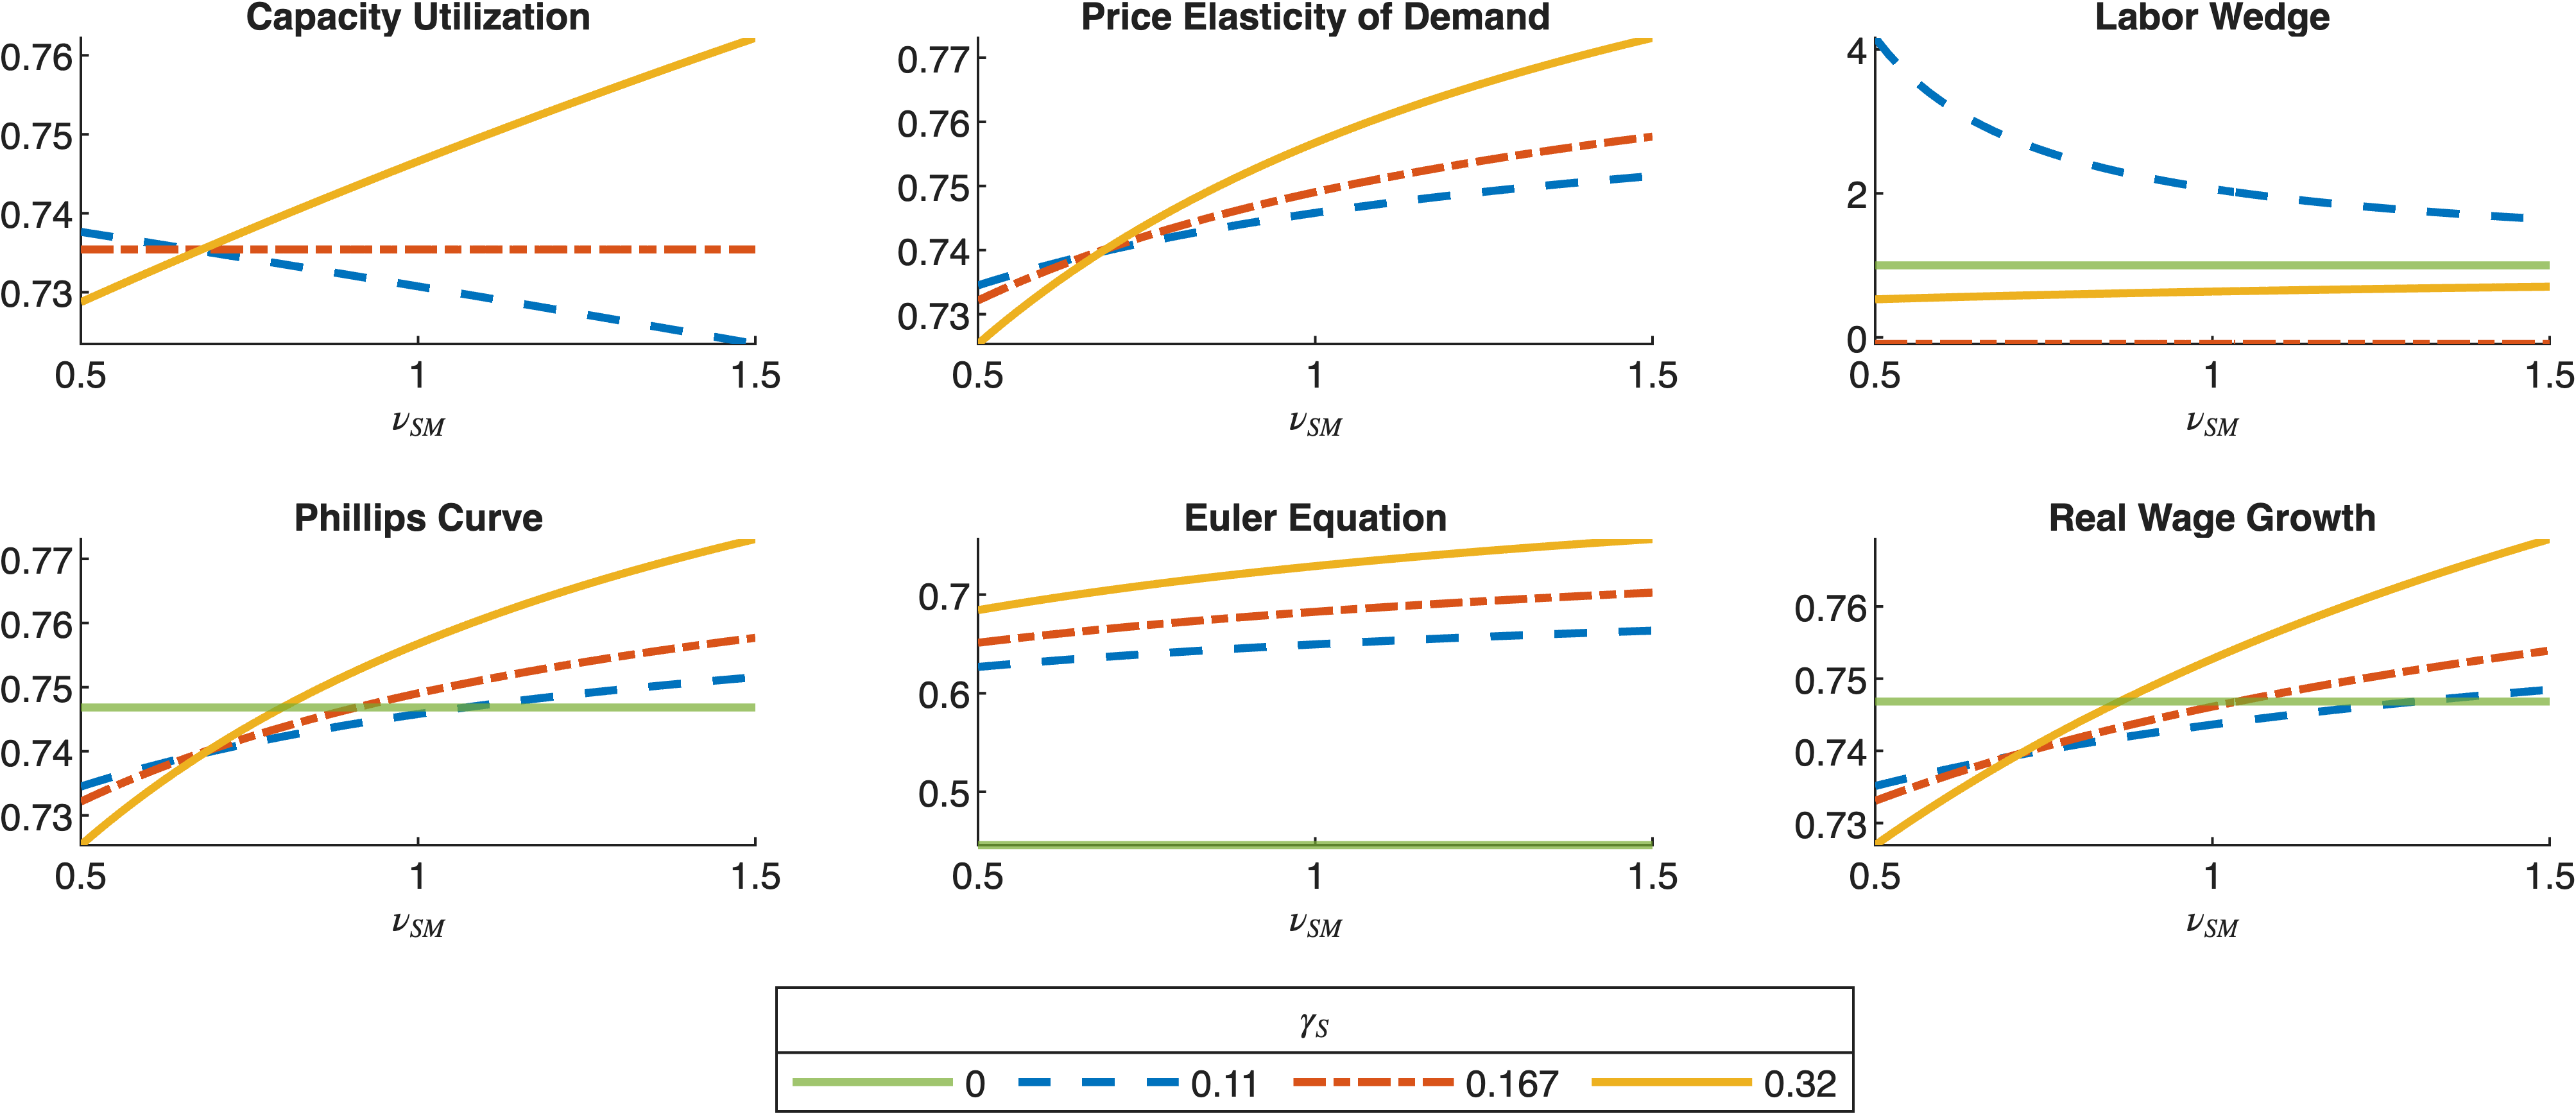
\includegraphics[width=\textwidth]{fig_18_slopes_robust_hw.png}\\%
    {\tiny \singlespacing NOTE: The graphs show the slopes of the NK-SaM model with home production relative to without home production. A value below one shows that the slope of a variable is smaller with home production compared to a model without home production. The figure shows how this ratio changes for different combinations of $\gamma_S$ and $\nu_{SM} = \nicefrac{\nu_S}{\nu_M}$.\par}%
\end{figure}%
% Statistics Table
\begin{table}[h!]%
	\begin{center}%
		\begin{footnotesize}%
			\caption{Dropping Home Production - Relative Standard Deviations and Correlations}\label{tab:app_robust_hw}%
			\begin{tabular}{l r r r r r r r r}%
				\hline%
				& \multicolumn{2}{c}{TFP} & \multicolumn{2}{c}{Policy} & \multicolumn{2}{c}{Cost-Push} & \multicolumn{2}{c}{Search}\\%
				Variable & Rel.Std. & Corr. & Rel.Std. & Corr. & Rel.Std. & Corr. & Rel.Std. & Corr.\\%
				\hline \hline%
				Output Gap & 0.05 & -0.44 & 1.00 & 1.00 & 0.39 & 0.92 & 0.09 & -0.97\\%
				UE Gap & 0.26 & -0.69 & 1.75 & -0.96 & 1.67 & -0.98 & 0.21 & -0.92\\%
				Inflation & 0.08 & -0.99 & 0.31 & 0.94 & 0.07 & -1.00 & 0.05 & -0.99\\%
				Real Wage & 0.63 & 0.90 & 2.26 & 0.81 & 1.30 & 0.82 & 0.23 & 0.86\\%
				Utilization & 0.74 & -0.99 & 0.76 & 0.68 & 0.96 & -1.00 & 0.67 & 1.00\\%
				Marginal Cost & 0.34 & -0.95 & 1.40 & 0.87 & 2.29 & 0.95 & 0.58 & -1.00\\%
				Price Elasticity & 0.81 & 0.95 & 3.30 & -0.87 & 18.43 & 0.98 & 1.37 & 1.00\\%
				Labor Wedge & 2.47 & 0.93 & 3.52 & -0.52 & 9.79 & -1.00 & 1.95 & 0.98\\%
				Search Effort & 0.85 & -0.97 & 2.66 & 0.86 & 1.36 & -1.00 & 2.65 & 1.00\\%
				\hline%
			\end{tabular}\\%
			\vspace{0.1in}%
			{\tiny NOTE: The table shows simulated second moments for the NK-SaM model. It shows relative standard deviations - standard deviation of each variable relative to standard deviation of real GDP - and correlations of each variable with real GDP. We consider each shock separately in the simulation.\par}%
		\end{footnotesize}%
	\end{center}%
\end{table}%
% IRF Figures - TFP and Demand Shocks
\begin{figure}[h!]%
    \centering%
    \caption{Dropping Home Production - IRFs to Expansionary TFP and Demand Shocks}\label{fig:app_irf_robust_hw_1}%
    \begin{subfigure}{\textwidth}%
        \centering%
        \caption{IRFs to an Expansionary TFP Shock}%
        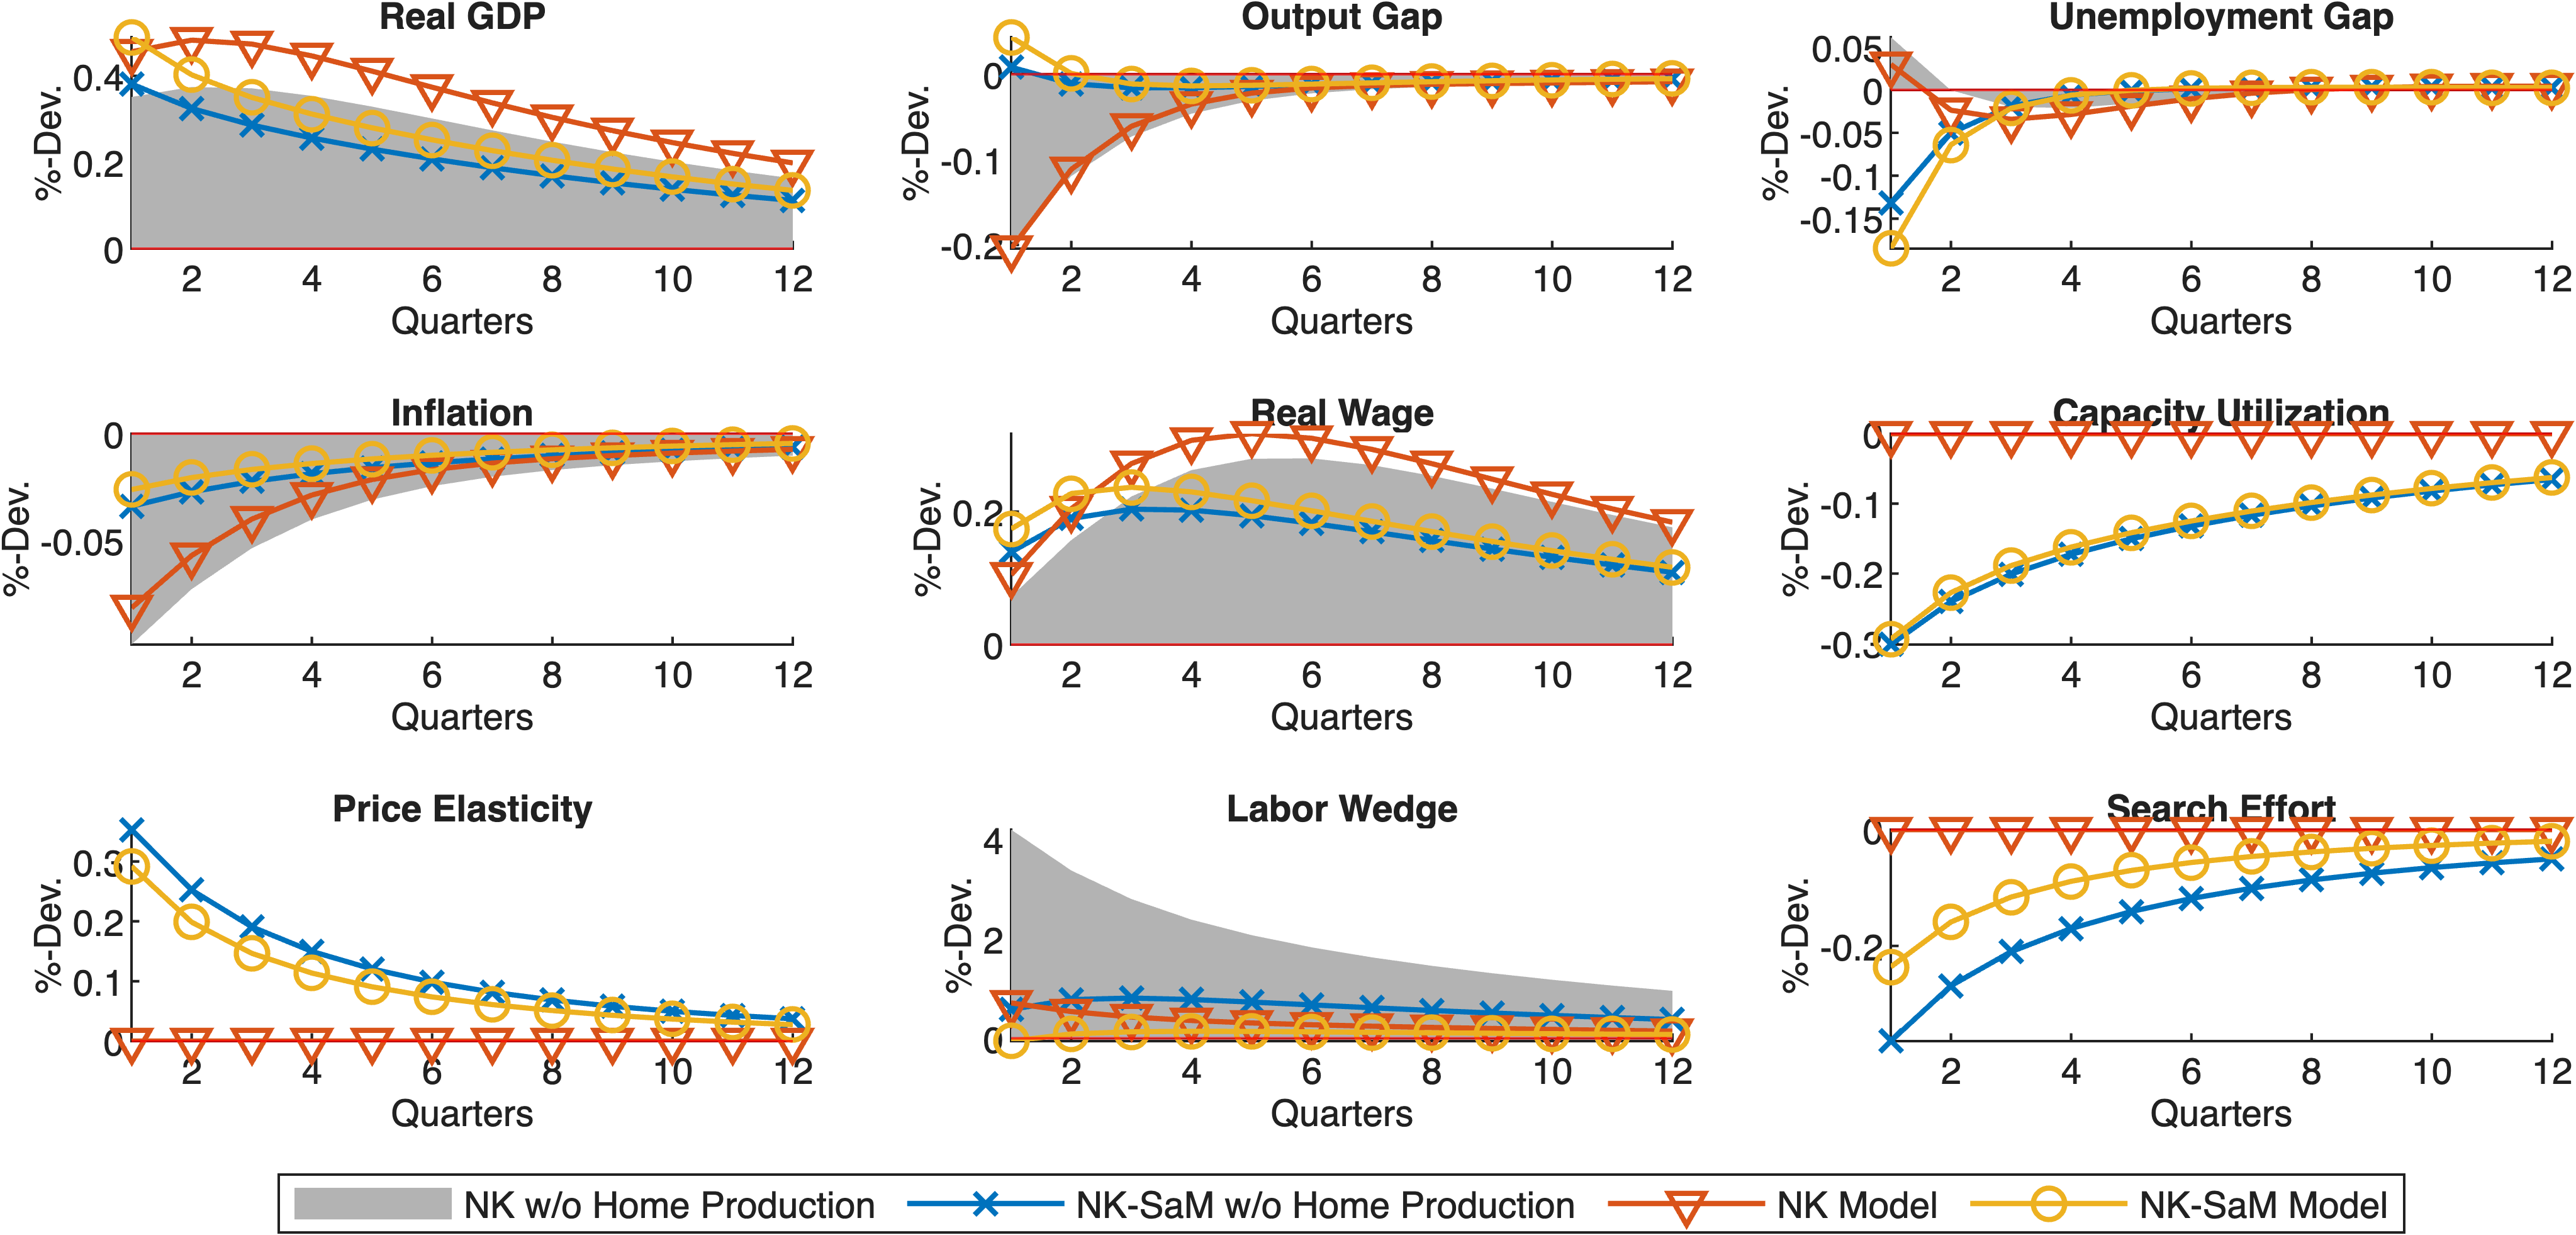
\includegraphics[width=\textwidth]{fig_19_irf_robust_comparison_tfp.png}%
    \end{subfigure}\\%
	\vspace{0.2in}%
    \begin{subfigure}{\textwidth}%
        \centering%
        \caption{IRFs to an Expansionary Monetary Policy Shock}%
        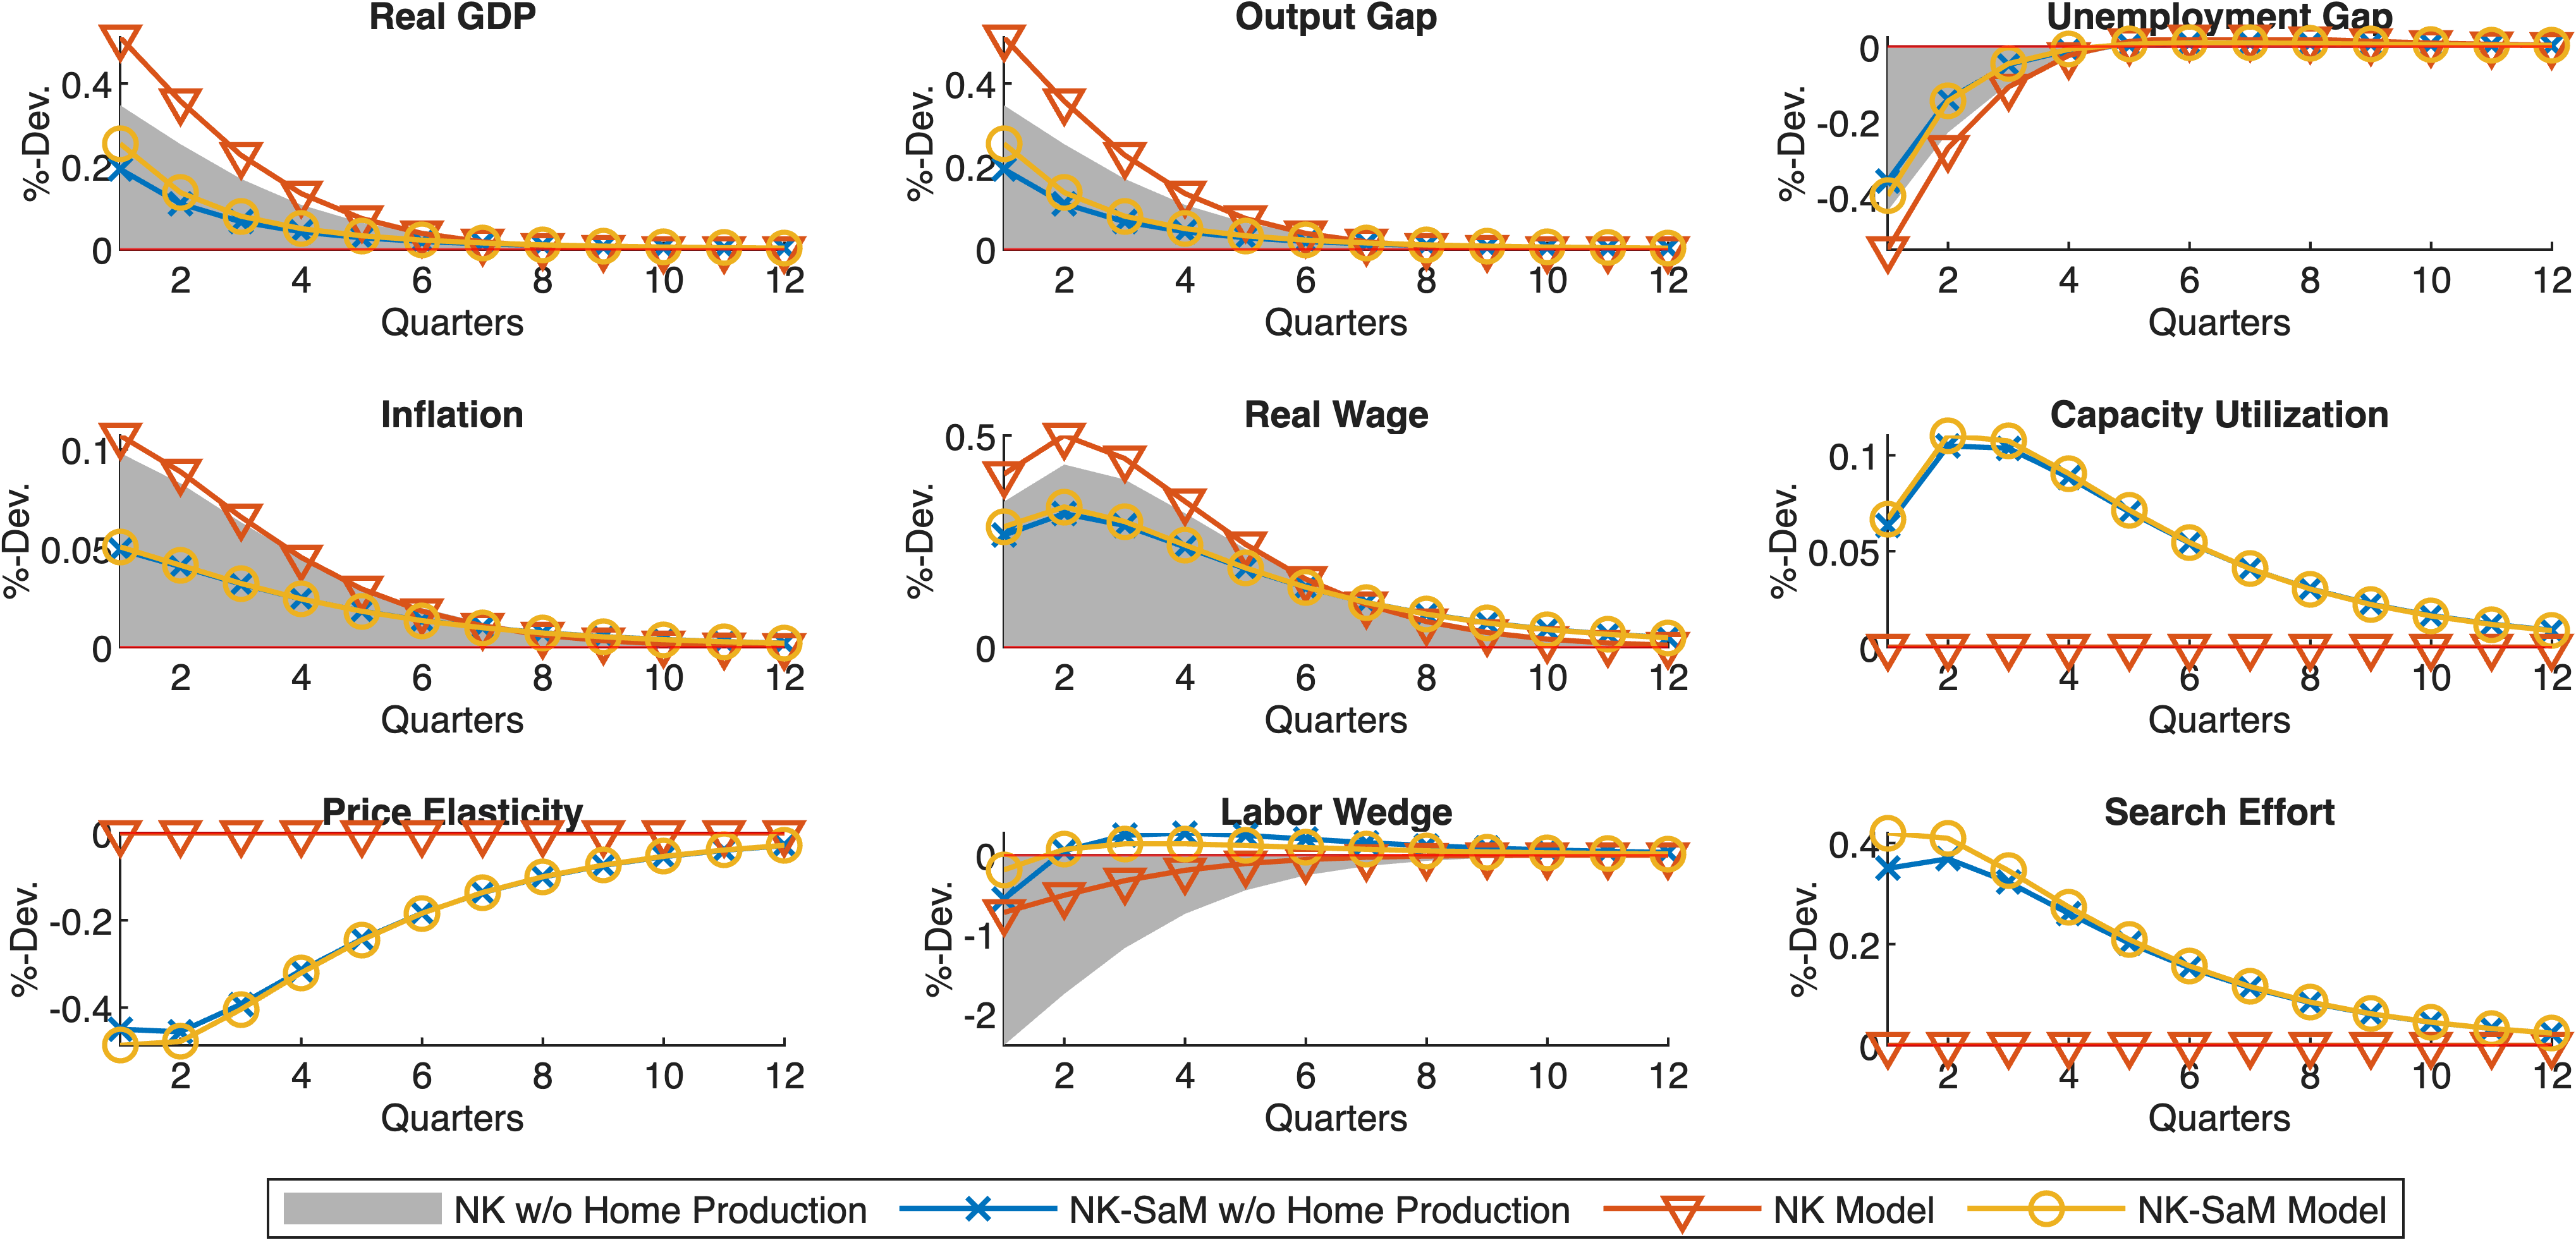
\includegraphics[width=\textwidth]{fig_20_irf_robust_comparison_policy.png}%
    \end{subfigure}\\%
    {\tiny \singlespacing NOTE: The figure shows IRFs to one standard deviation expansionary shocks using the model presented in \cref{sec:model} and \cref{sec:dynamics}. The models are calibrated as given in the legend.\par}%
\end{figure}%
% IRF FIGURES - COST PUSH SHOCKS
\begin{figure}[h!]%
    \centering%
    \caption{Dropping Home Production - IRFs to Expansionary Cost Push Shocks}\label{fig:app_irf_robust_hw_2}%
    \begin{subfigure}{\textwidth}%
        \centering%
        \caption{IRFs to an Expansionary EIS Shock}%
        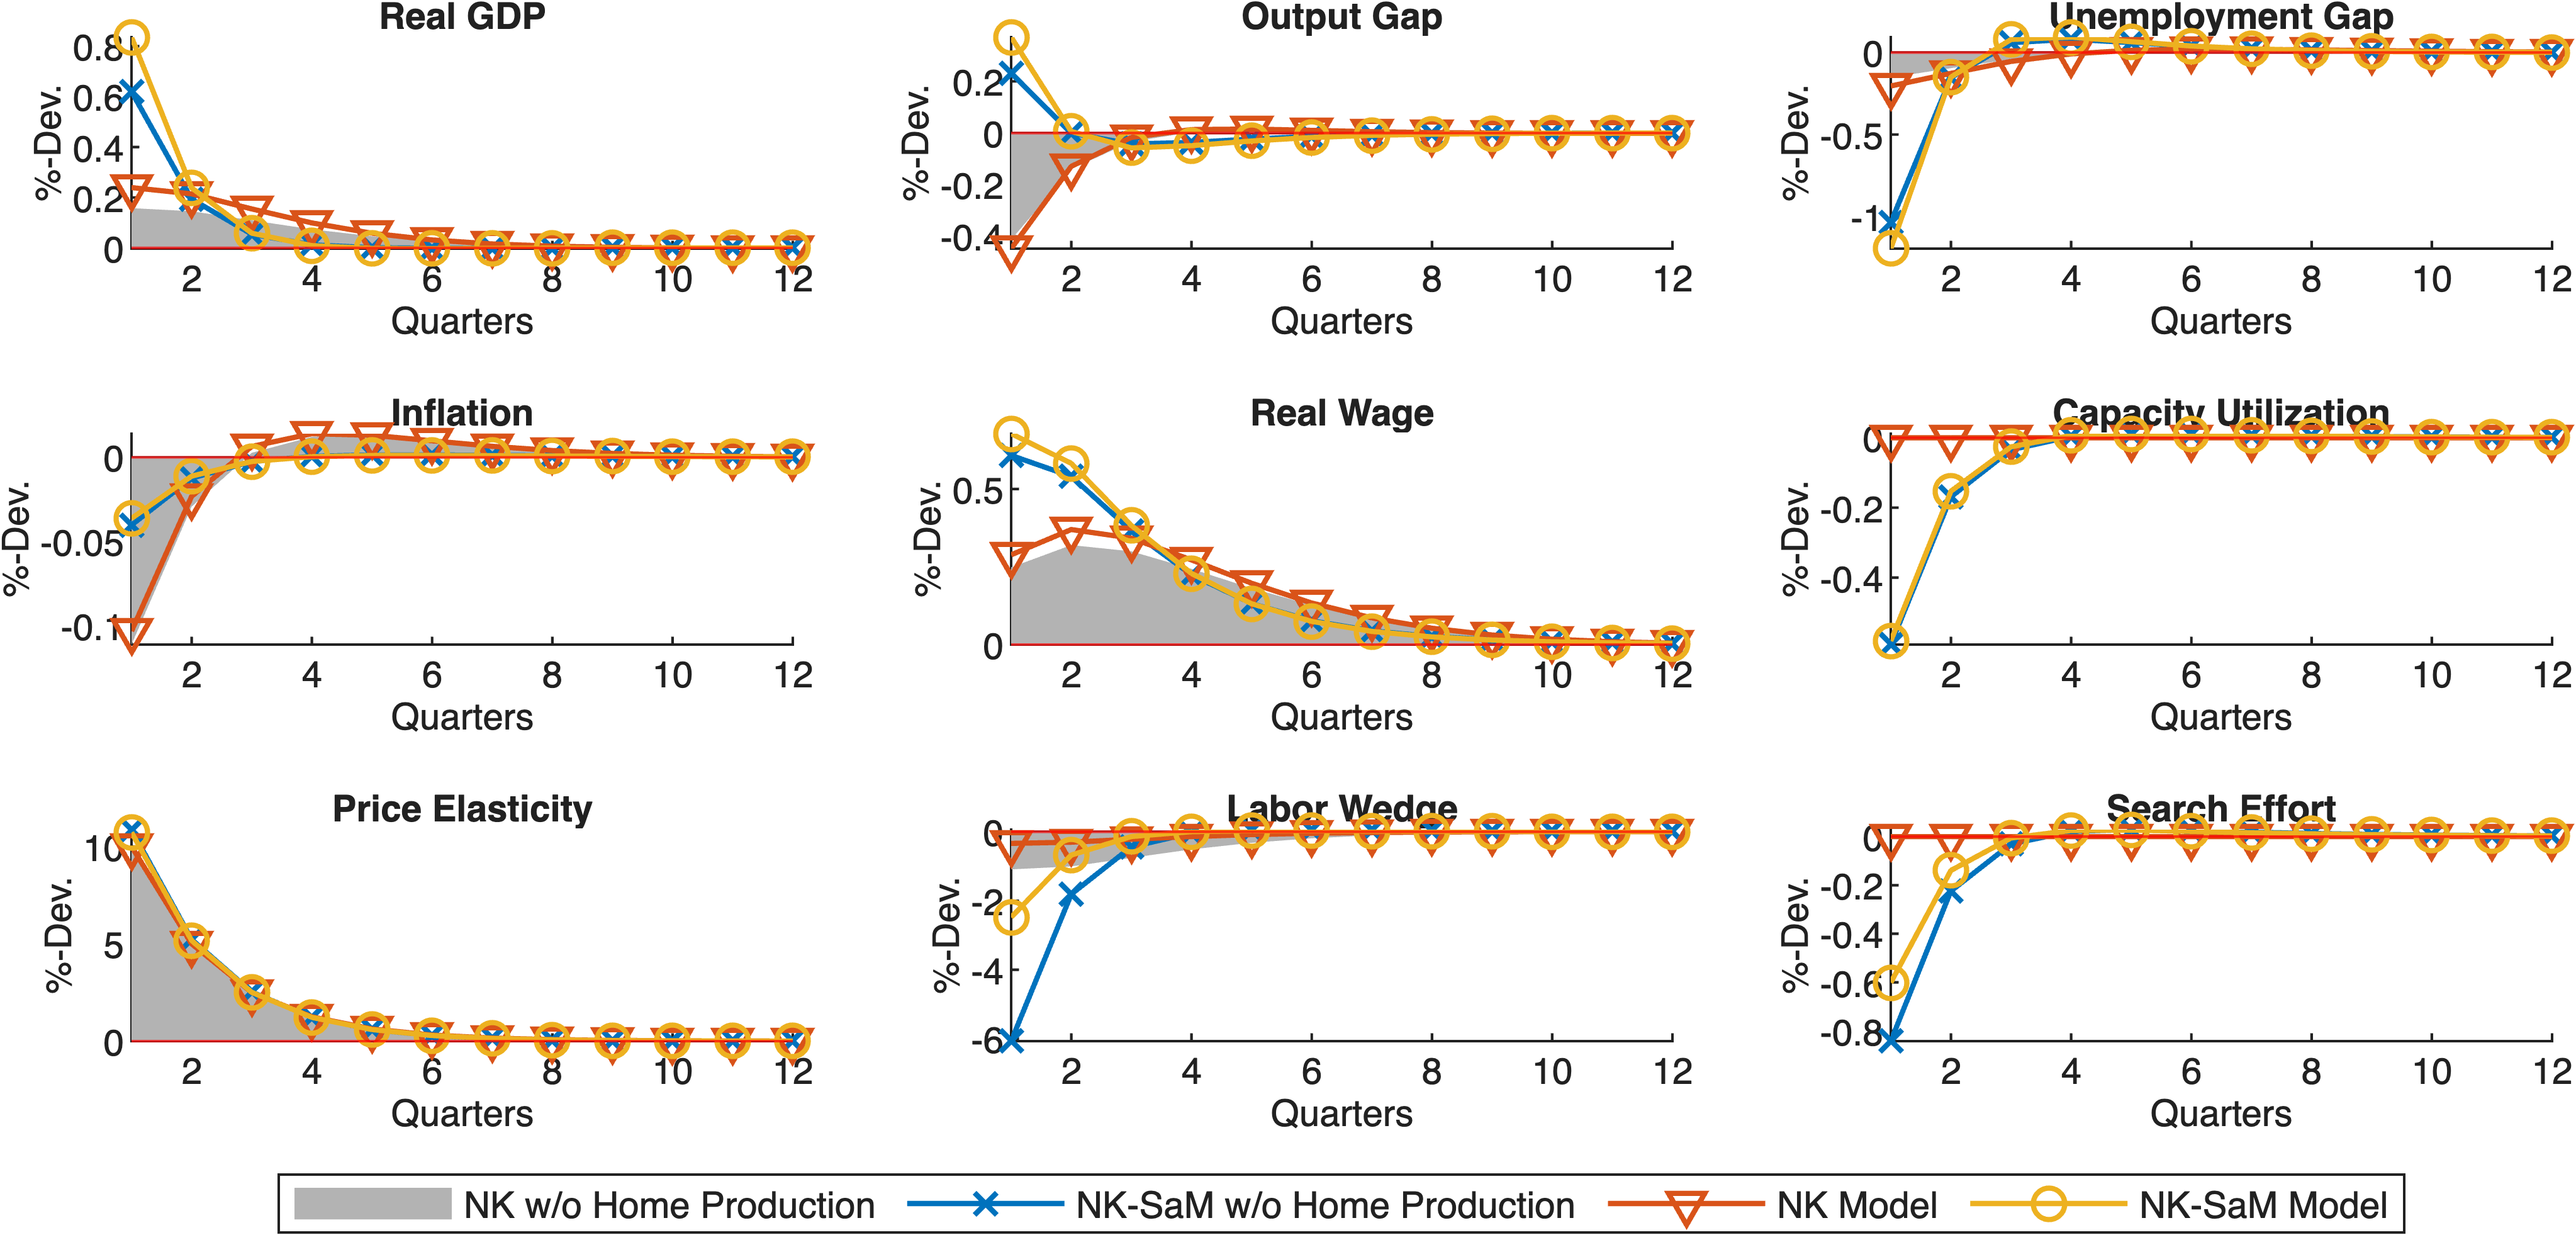
\includegraphics[width=\textwidth]{fig_21_irf_robust_comparison_eis.png}%
    \end{subfigure}\\%
	\vspace{0.2in}%
    \begin{subfigure}{\textwidth}%
        \centering%
        \caption{IRFs to an Expansionary Search Effort Shock}%
        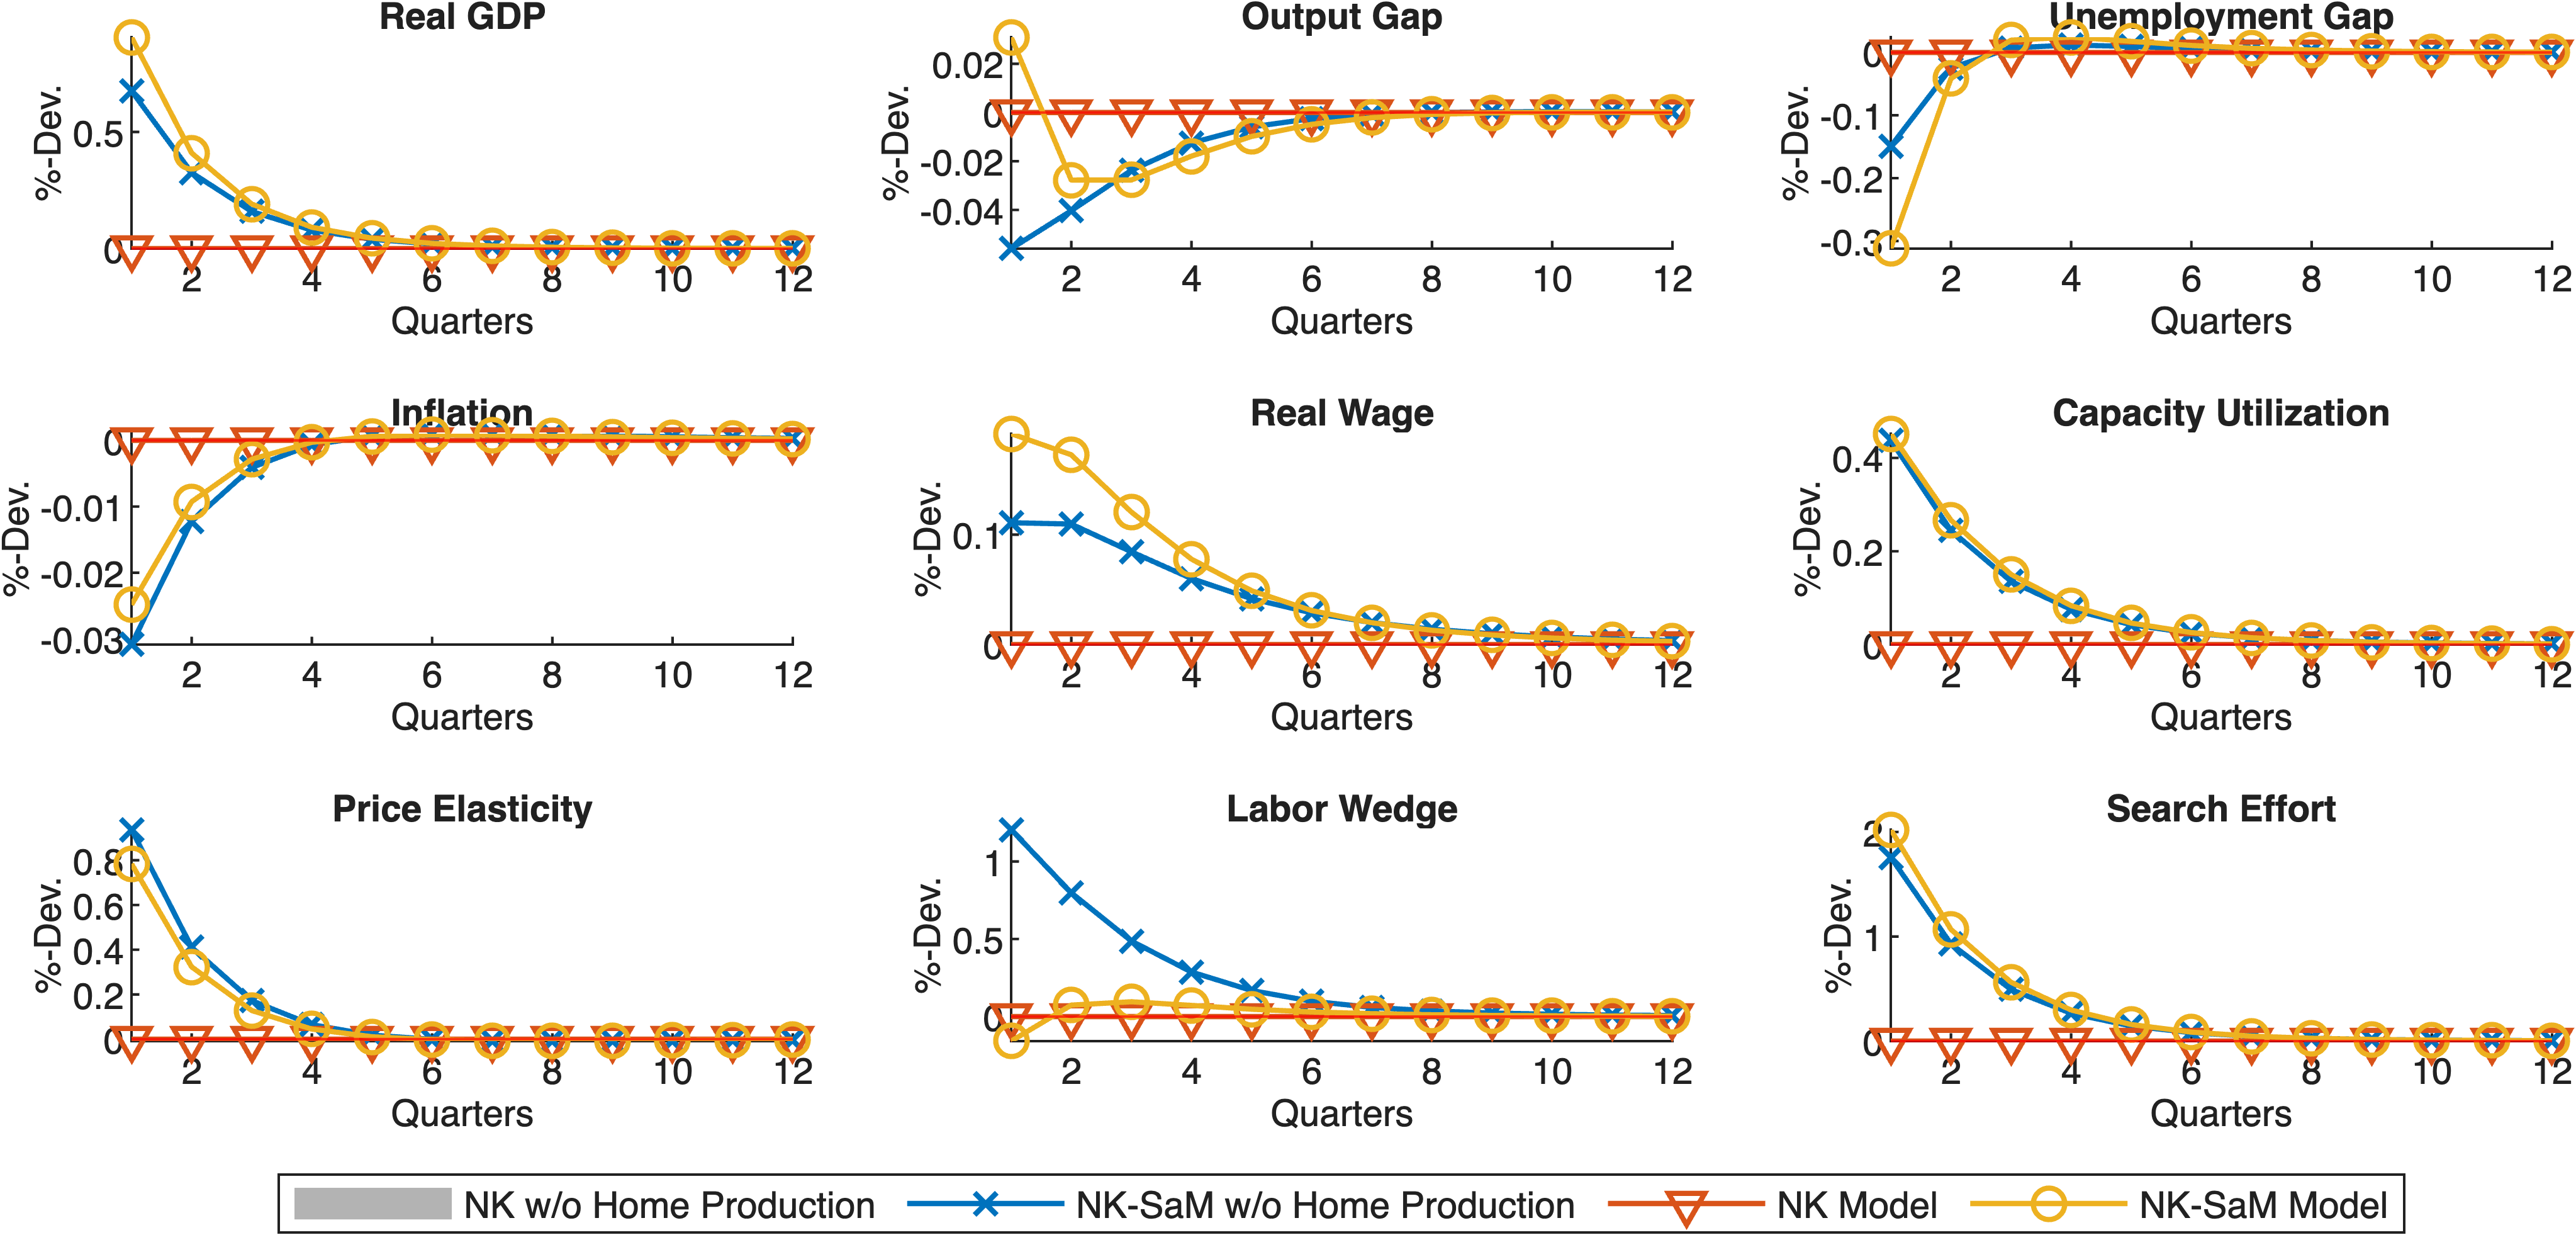
\includegraphics[width=\textwidth]{fig_22_irf_robust_comparison_search.png}%
    \end{subfigure}\\%
    {\tiny \singlespacing NOTE: The figure shows IRFs to one standard deviation expansionary shocks using the model presented in \cref{sec:model} and \cref{sec:dynamics}. The models are calibrated as given in the legend.\par}%
\end{figure}%
% ROBUSTNESS: GHH PREFERENCES
%-----------------------------------------------------------
\FloatBarrier%
\subsection{Robustness - \cite{greenwoodInvestmentCapacityUtilization1988} Preferences}\label{sec:robust_ghh}%
% Slopes Figure
\begin{figure}[h!]%
    \centering%
    \caption{Relative Slopes - GHH Preferences relative to KPR Preferences}\label{fig:app_slopes_robust_ghh}%
    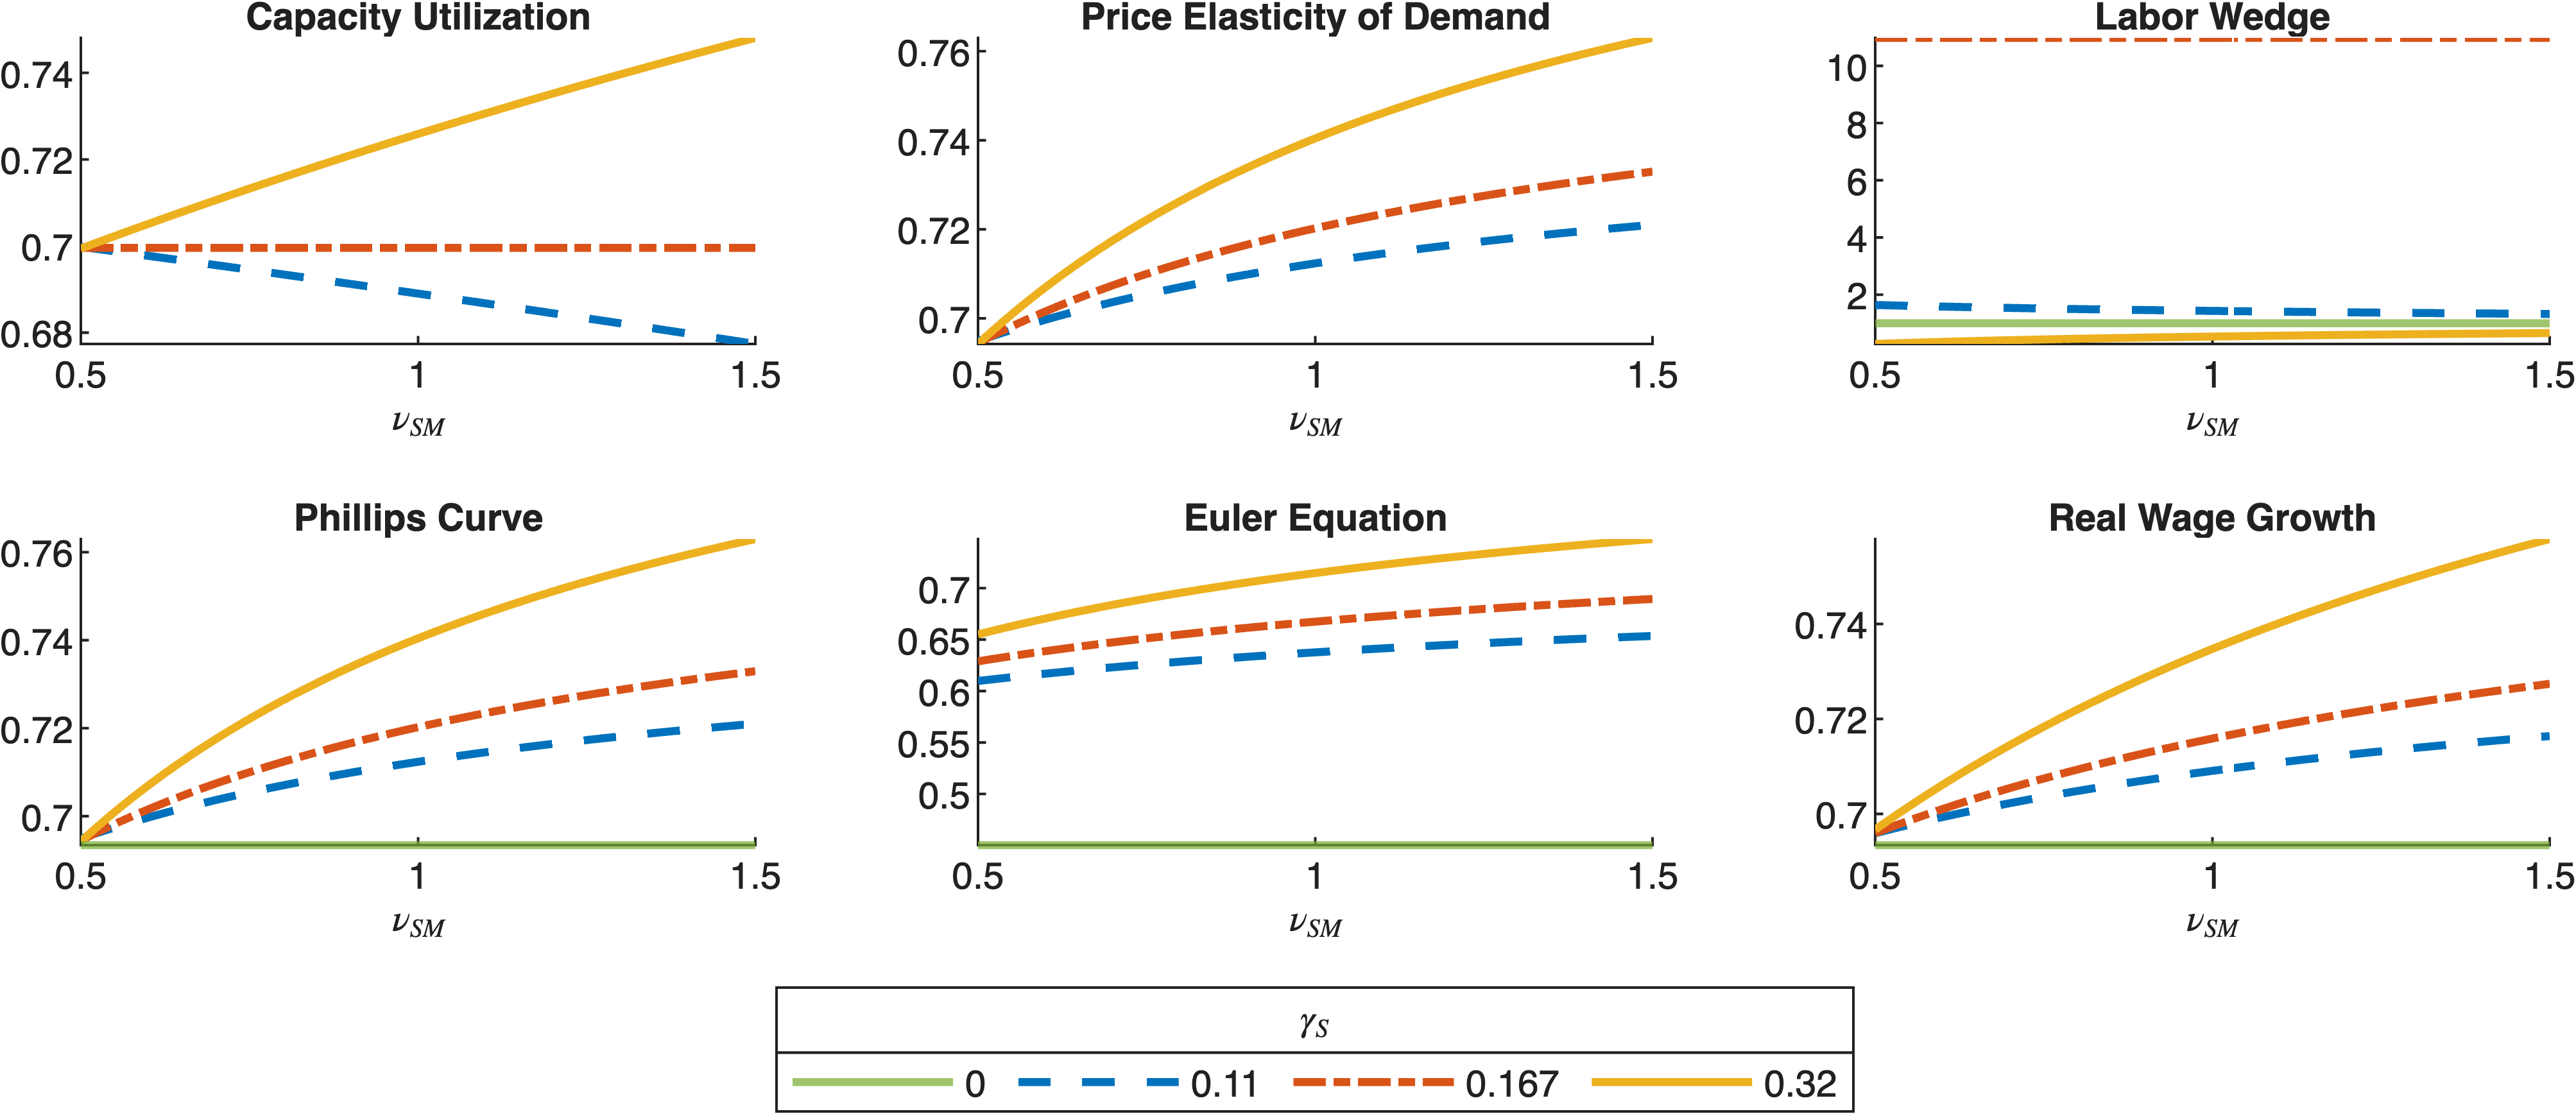
\includegraphics[width=\textwidth]{fig_23_slopes_robust_ghh.png}\\%
    {\tiny \singlespacing NOTE: The graphs show the slopes of the NK-SaM model with GHH preferencs relative to KPR preferences. A value below one shows that the slope of a variable is smaller with GHH preferences compared to a model witho KPR preferences. The figure shows how this ratio changes for different combinations of $\gamma_S$ and $\nu_{SM} = \nicefrac{\nu_S}{\nu_M}$.\par}%
\end{figure}%
% Statistics Table
\begin{table}[h!]%
	\begin{center}%
		\begin{footnotesize}%
			\caption{Using GHH Preferences - Relative Standard Deviations and Correlations}\label{tab:app_robust_ghh}%
			\begin{tabular}{l r r r r r r r r}%
				\hline%
				& \multicolumn{2}{c}{TFP} & \multicolumn{2}{c}{Policy} & \multicolumn{2}{c}{Cost-Push} & \multicolumn{2}{c}{Search}\\%
				Variable & Rel.Std. & Corr. & Rel.Std. & Corr. & Rel.Std. & Corr. & Rel.Std. & Corr.\\%
				\hline \hline%
				Output Gap & 0.06 & -0.74 & 1.00 & 1.00 & 0.53 & 0.96 & 0.21 & -0.99\\%
				UE Gap & 0.15 & -0.67 & 1.15 & -0.96 & 1.12 & -0.98 & 0.01 & -0.71\\%
				Inflation & 0.06 & -0.99 & 0.17 & 0.93 & 0.03 & -1.00 & 0.04 & -0.98\\%
				Real Wage & 0.37 & 0.89 & 1.31 & 0.79 & 0.77 & 0.82 & 0.08 & 0.63\\%
				Utilization & 0.49 & -0.99 & 0.43 & 0.64 & 0.45 & -1.00 & 0.45 & 1.00\\%
				Marginal Cost & 0.25 & -0.96 & 0.82 & 0.87 & 1.23 & 0.94 & 0.47 & -1.00\\%
				Price Elasticity & 0.58 & 0.96 & 1.94 & -0.87 & 8.77 & 0.96 & 1.11 & 1.00\\%
				Labor Wedge & 0.12 & -0.70 & 0.43 & -0.66 & 1.00 & -1.00 & 0.12 & -0.99\\%
				Search Effort & 0.25 & -0.83 & 1.88 & 0.90 & 0.11 & -0.96 & 2.11 & 1.00\\%
				\hline%
			\end{tabular}\\%
			\vspace{0.1in}%
			{\tiny NOTE: The table shows simulated second moments for the NK-SaM model. It shows relative standard deviations - standard deviation of each variable relative to standard deviation of real GDP - and correlations of each variable with real GDP. We consider each shock separately in the simulation.\par}%
		\end{footnotesize}%
	\end{center}%
\end{table}%
% IRF Figures - TFP AND DEMAND SHOCKS
\begin{figure}[h!]%
    \centering%
    \caption{Using GHH Preferences - IRFs to Expansionary TFP and Demand Shocks}\label{fig:app_irf_robust_ghh_1}%
    \begin{subfigure}{\textwidth}%
        \centering%
        \caption{IRFs to an Expansionary TFP Shock}%
        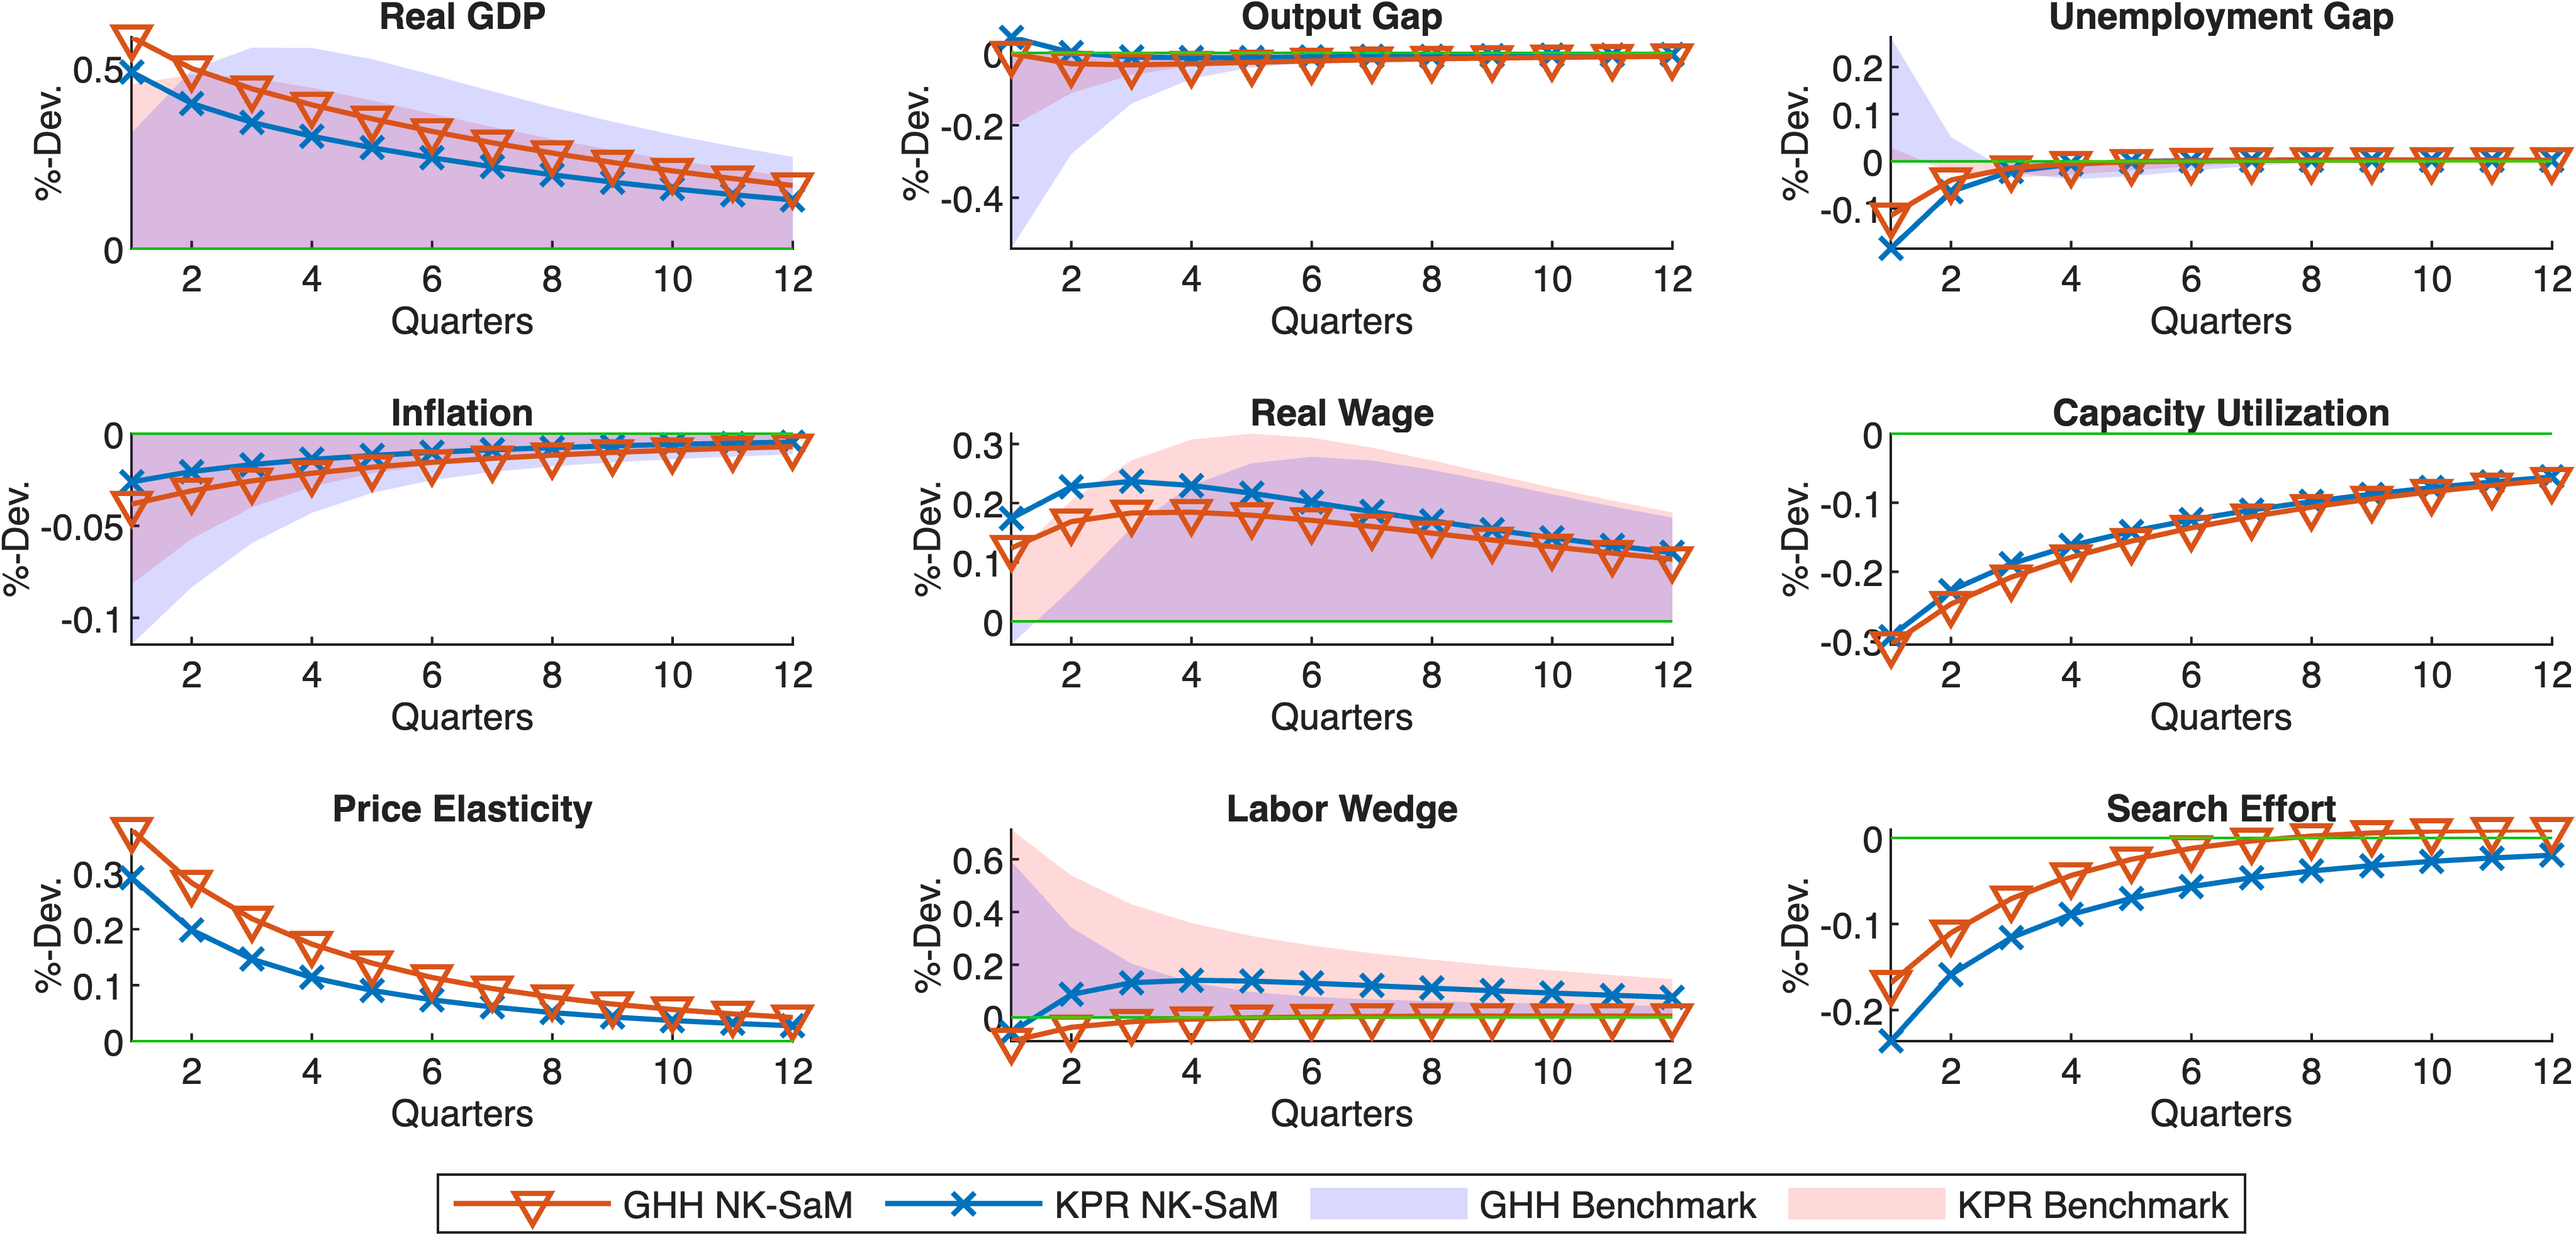
\includegraphics[width=\textwidth]{fig_24_irf_robust_ghh_tfp.png}%
    \end{subfigure}\\%
	\vspace{0.2in}%
    \begin{subfigure}{\textwidth}%
        \centering%
        \caption{IRFs to an Expansionary Monetary Policy Shock}%
        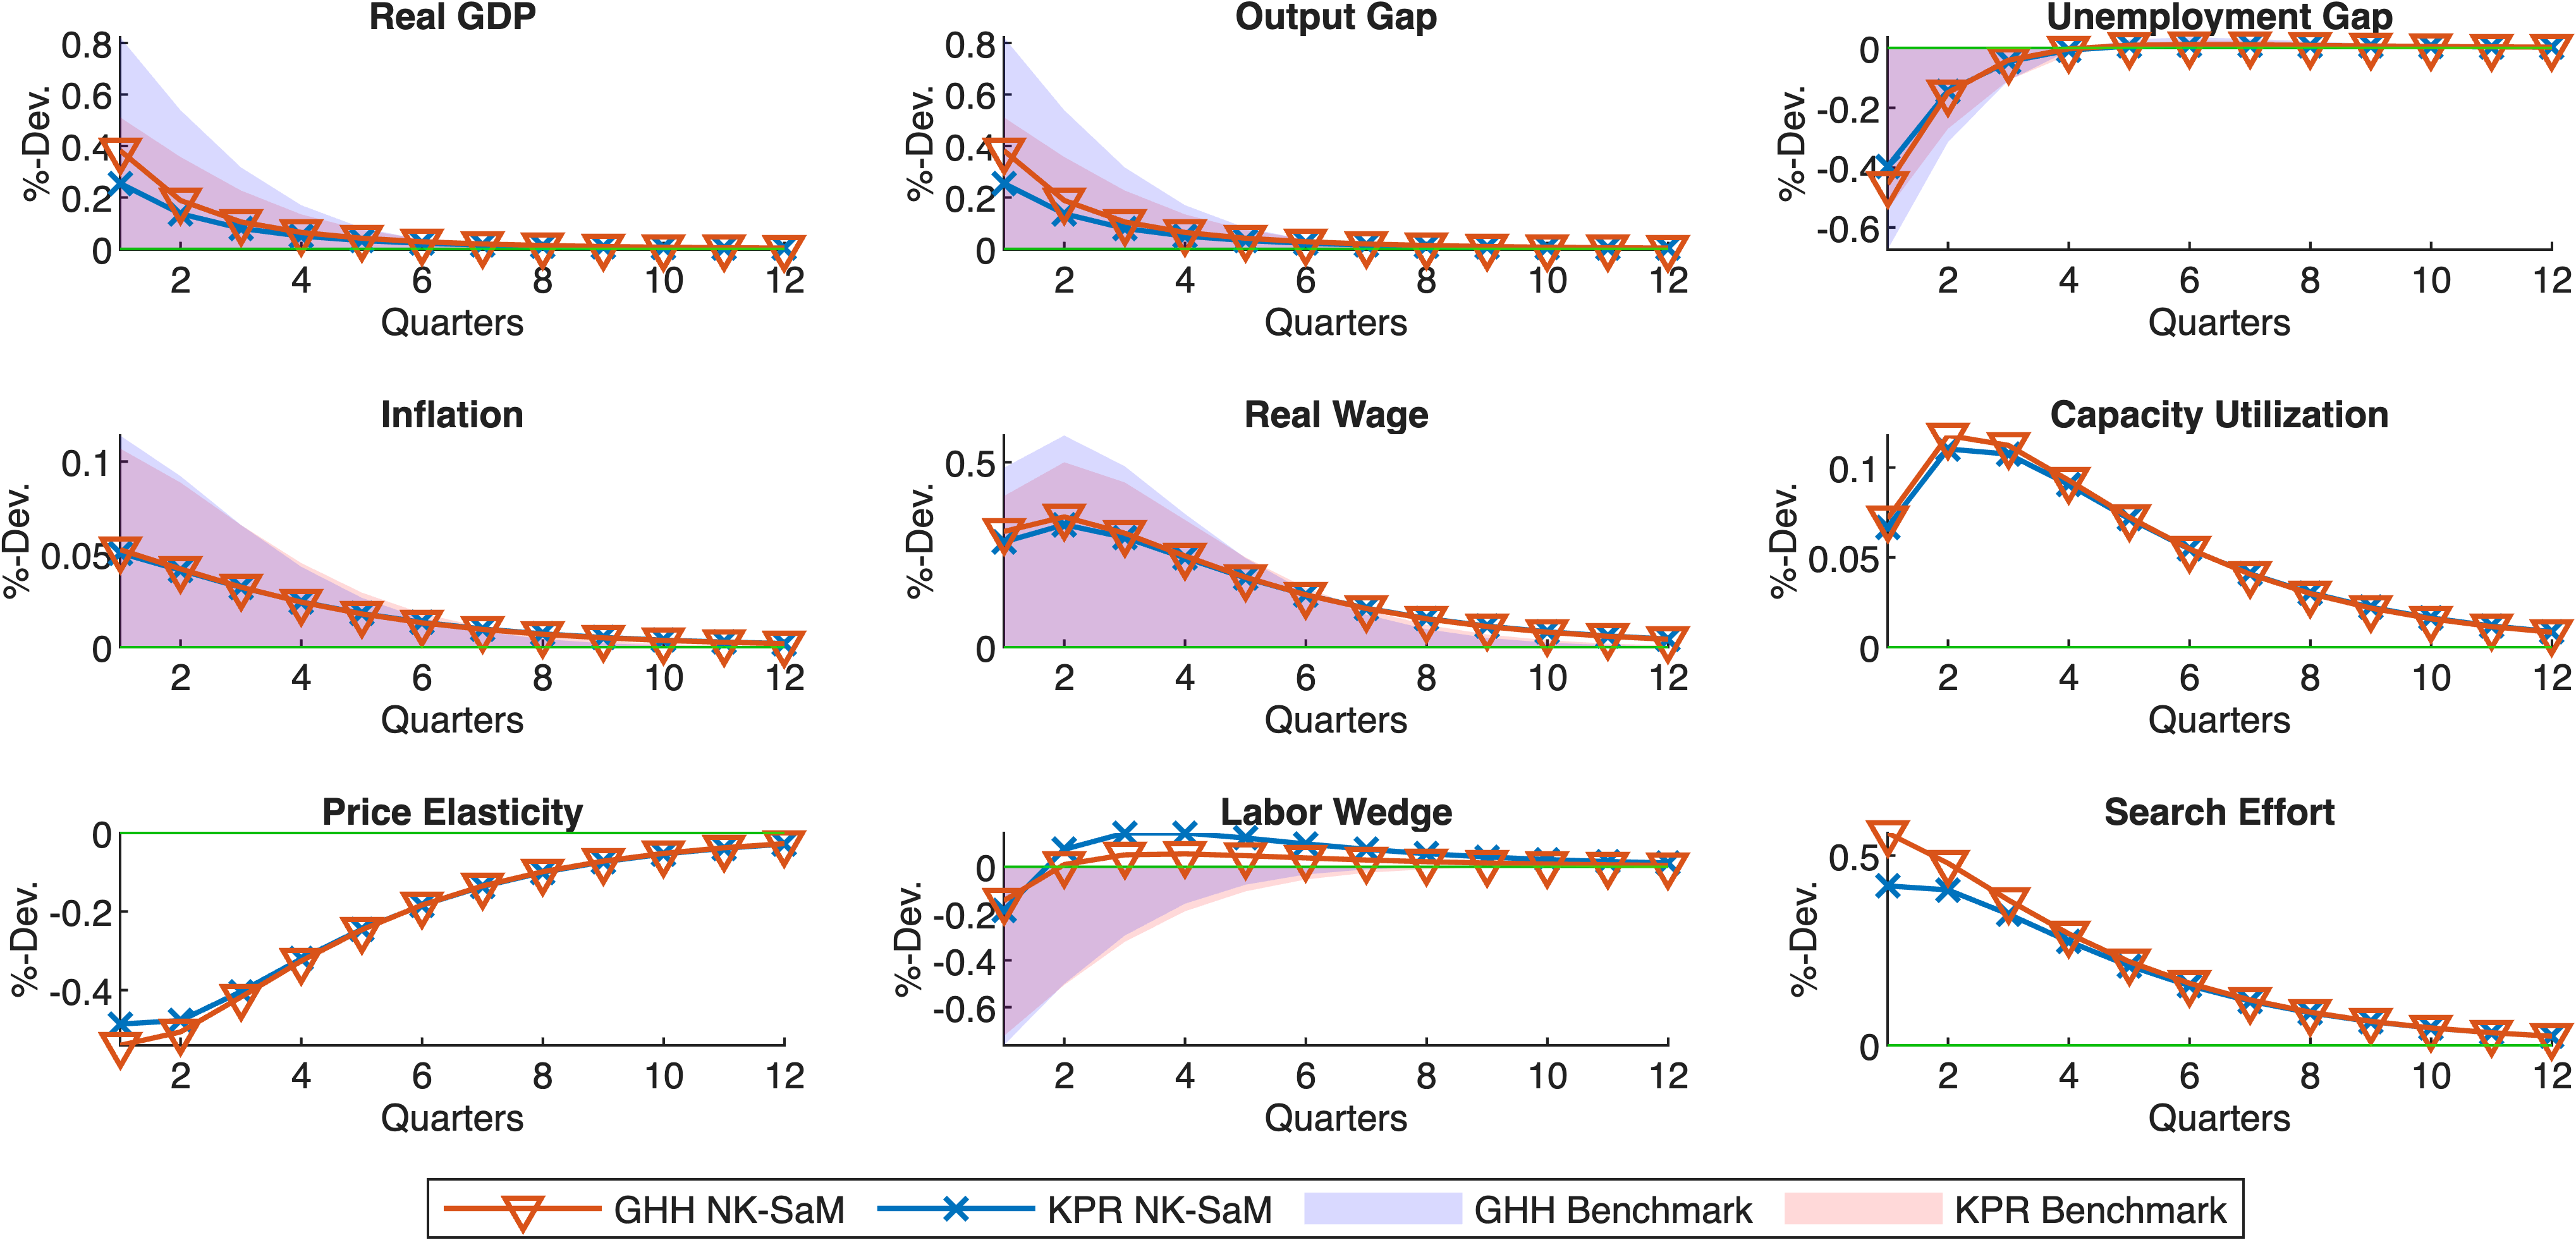
\includegraphics[width=\textwidth]{fig_25_irf_robust_ghh_policy.png}%
    \end{subfigure}\\%
    {\tiny \singlespacing NOTE: The figure shows IRFs to one standard deviation expansionary shocks using the model presented in \cref{sec:model} and \cref{sec:dynamics}. The models are calibrated as given in the legend.\par}%
\end{figure}%
% IRF Figures - COST PUSH SHOCKS
\begin{figure}[h!]%
    \centering%
    \caption{Using GHH Preferences - IRFs to Expansionary Cost Push Shocks}\label{fig:app_irf_robust_ghh_2}%
    \begin{subfigure}{\textwidth}%
        \centering%
        \caption{IRFs to an Expansionary EIS Shock}%
        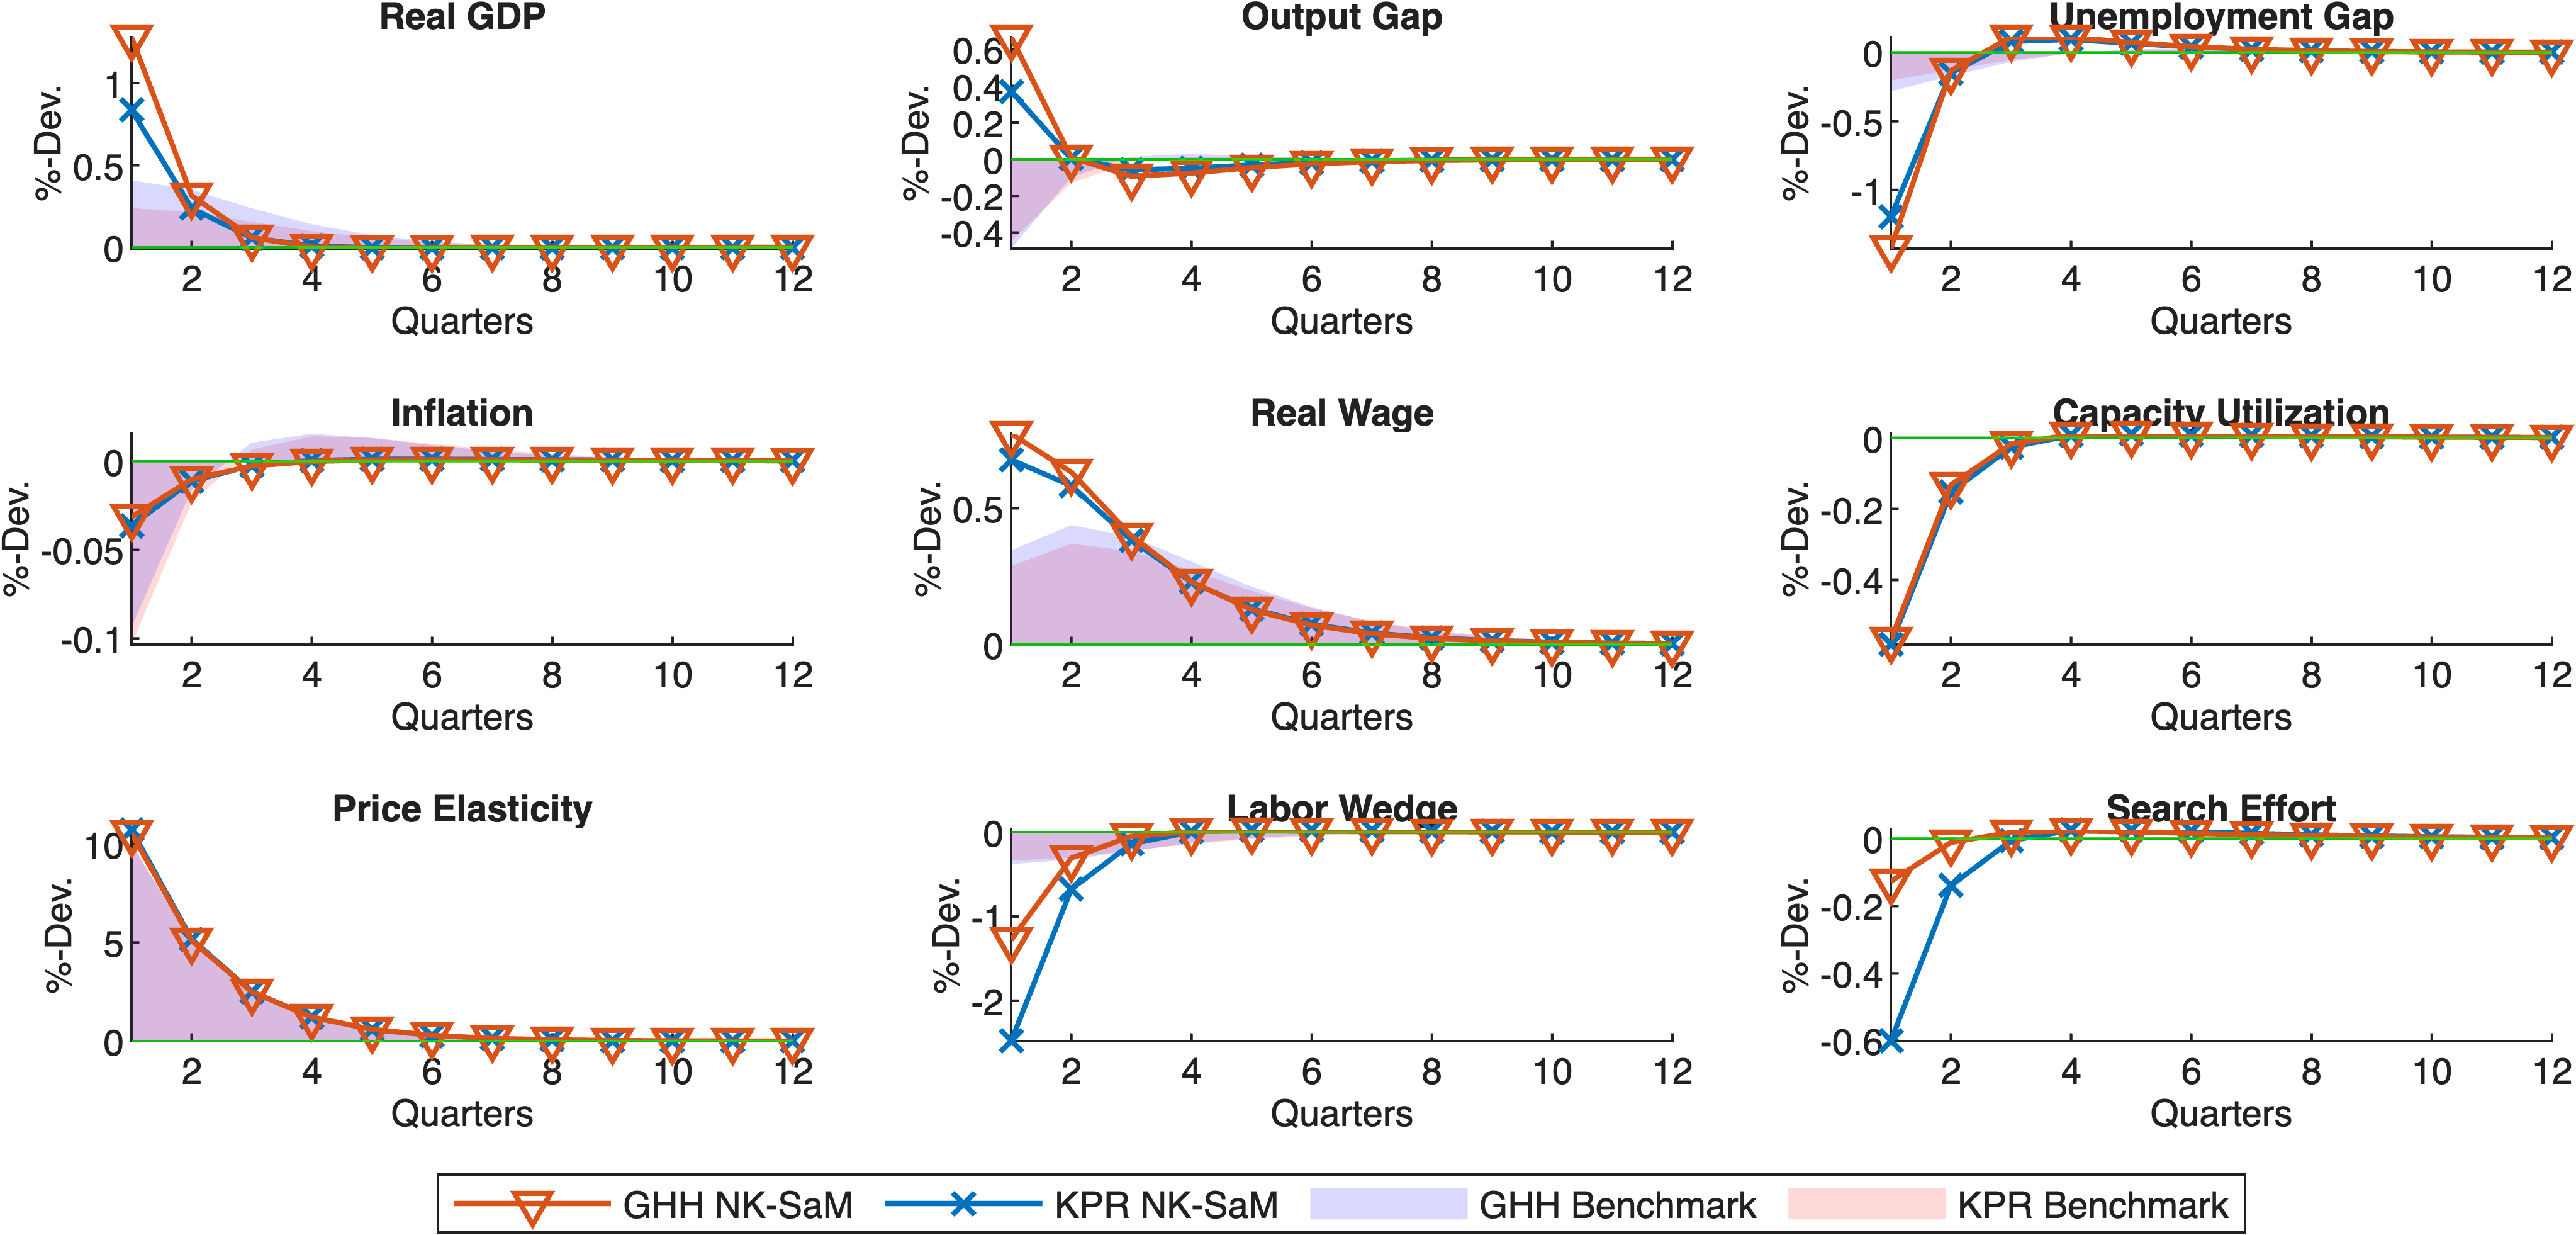
\includegraphics[width=\textwidth]{fig_26_irf_robust_ghh_eis.png}%
    \end{subfigure}\\%
	\vspace{0.2in}%
    \begin{subfigure}{\textwidth}%
        \centering%
        \caption{IRFs to an Expansionary Search Effort Shock}%
        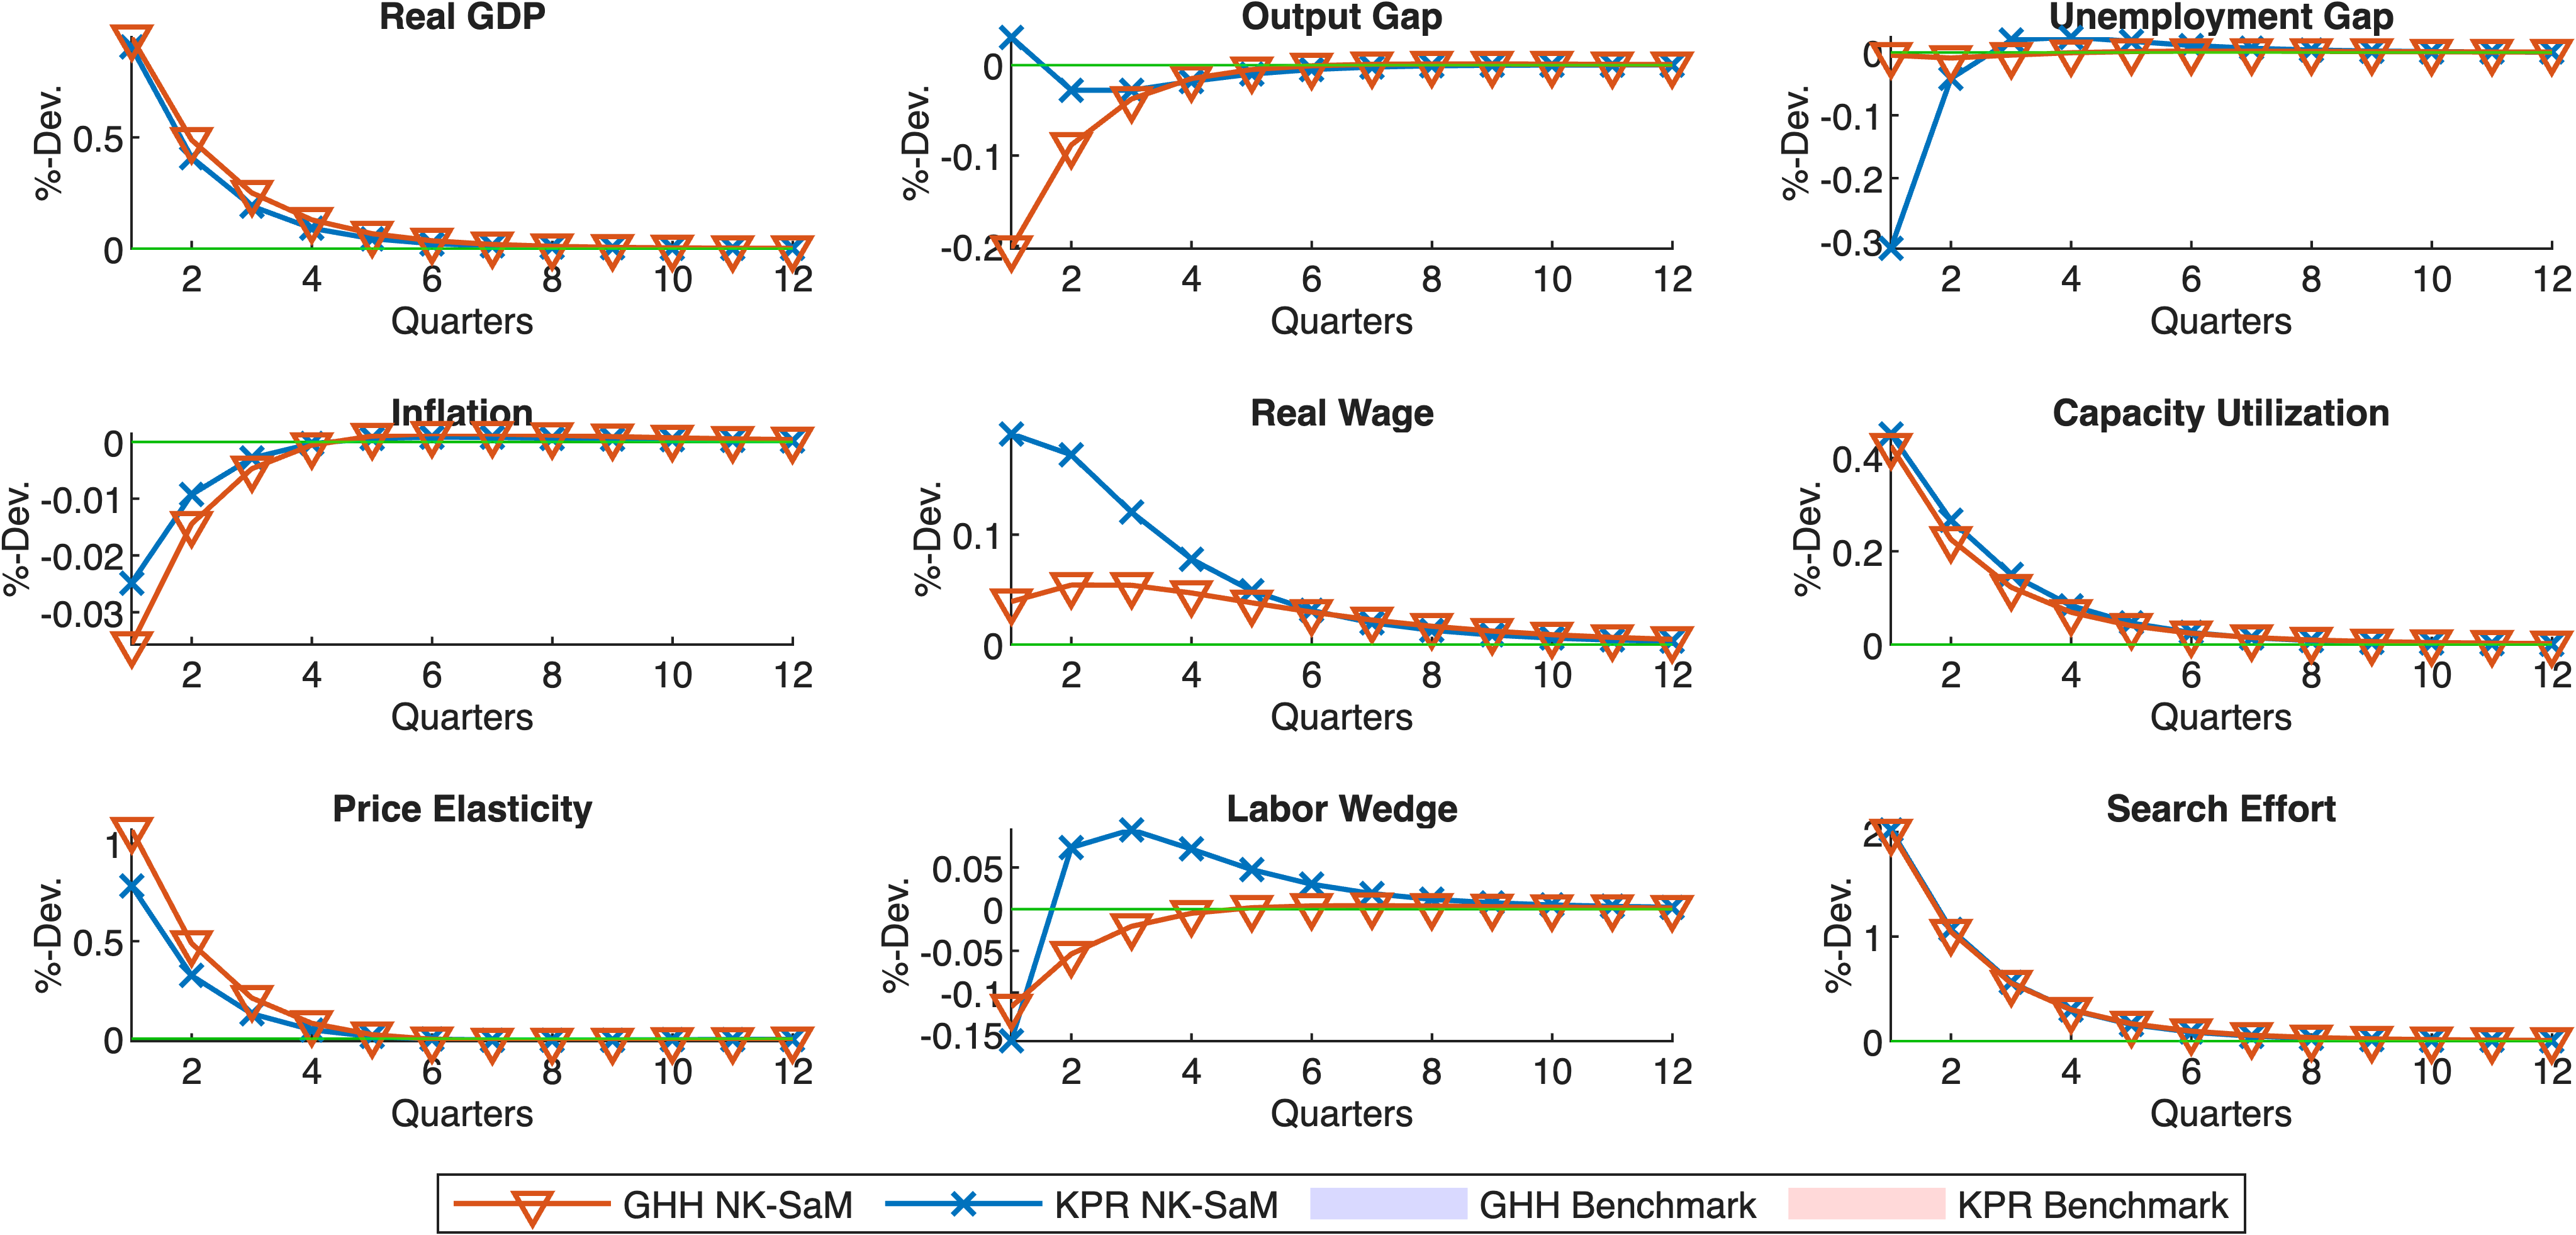
\includegraphics[width=\textwidth]{fig_27_irf_robust_ghh_search.png}%
    \end{subfigure}\\%
    {\tiny \singlespacing NOTE: The figure shows IRFs to one standard deviation expansionary shocks using the model presented in \cref{sec:model} and \cref{sec:dynamics}. The models are calibrated as given in the legend.\par}%
\end{figure}%
% ROBUSTNESS: NOMINAL WAGE ADJUSTMENT COSTS
%-----------------------------------------------------------
\FloatBarrier%
\subsection{Robustness - Nominal Wage Adjustment Costs}\label{sec:robust_wages}%
% Slopes Figure
\begin{figure}[h!]%
    \centering%
    \caption{Relative Slopes - Sticky Wages relative to Felxible Wages}\label{fig:app_slopes_robust_sw}%
    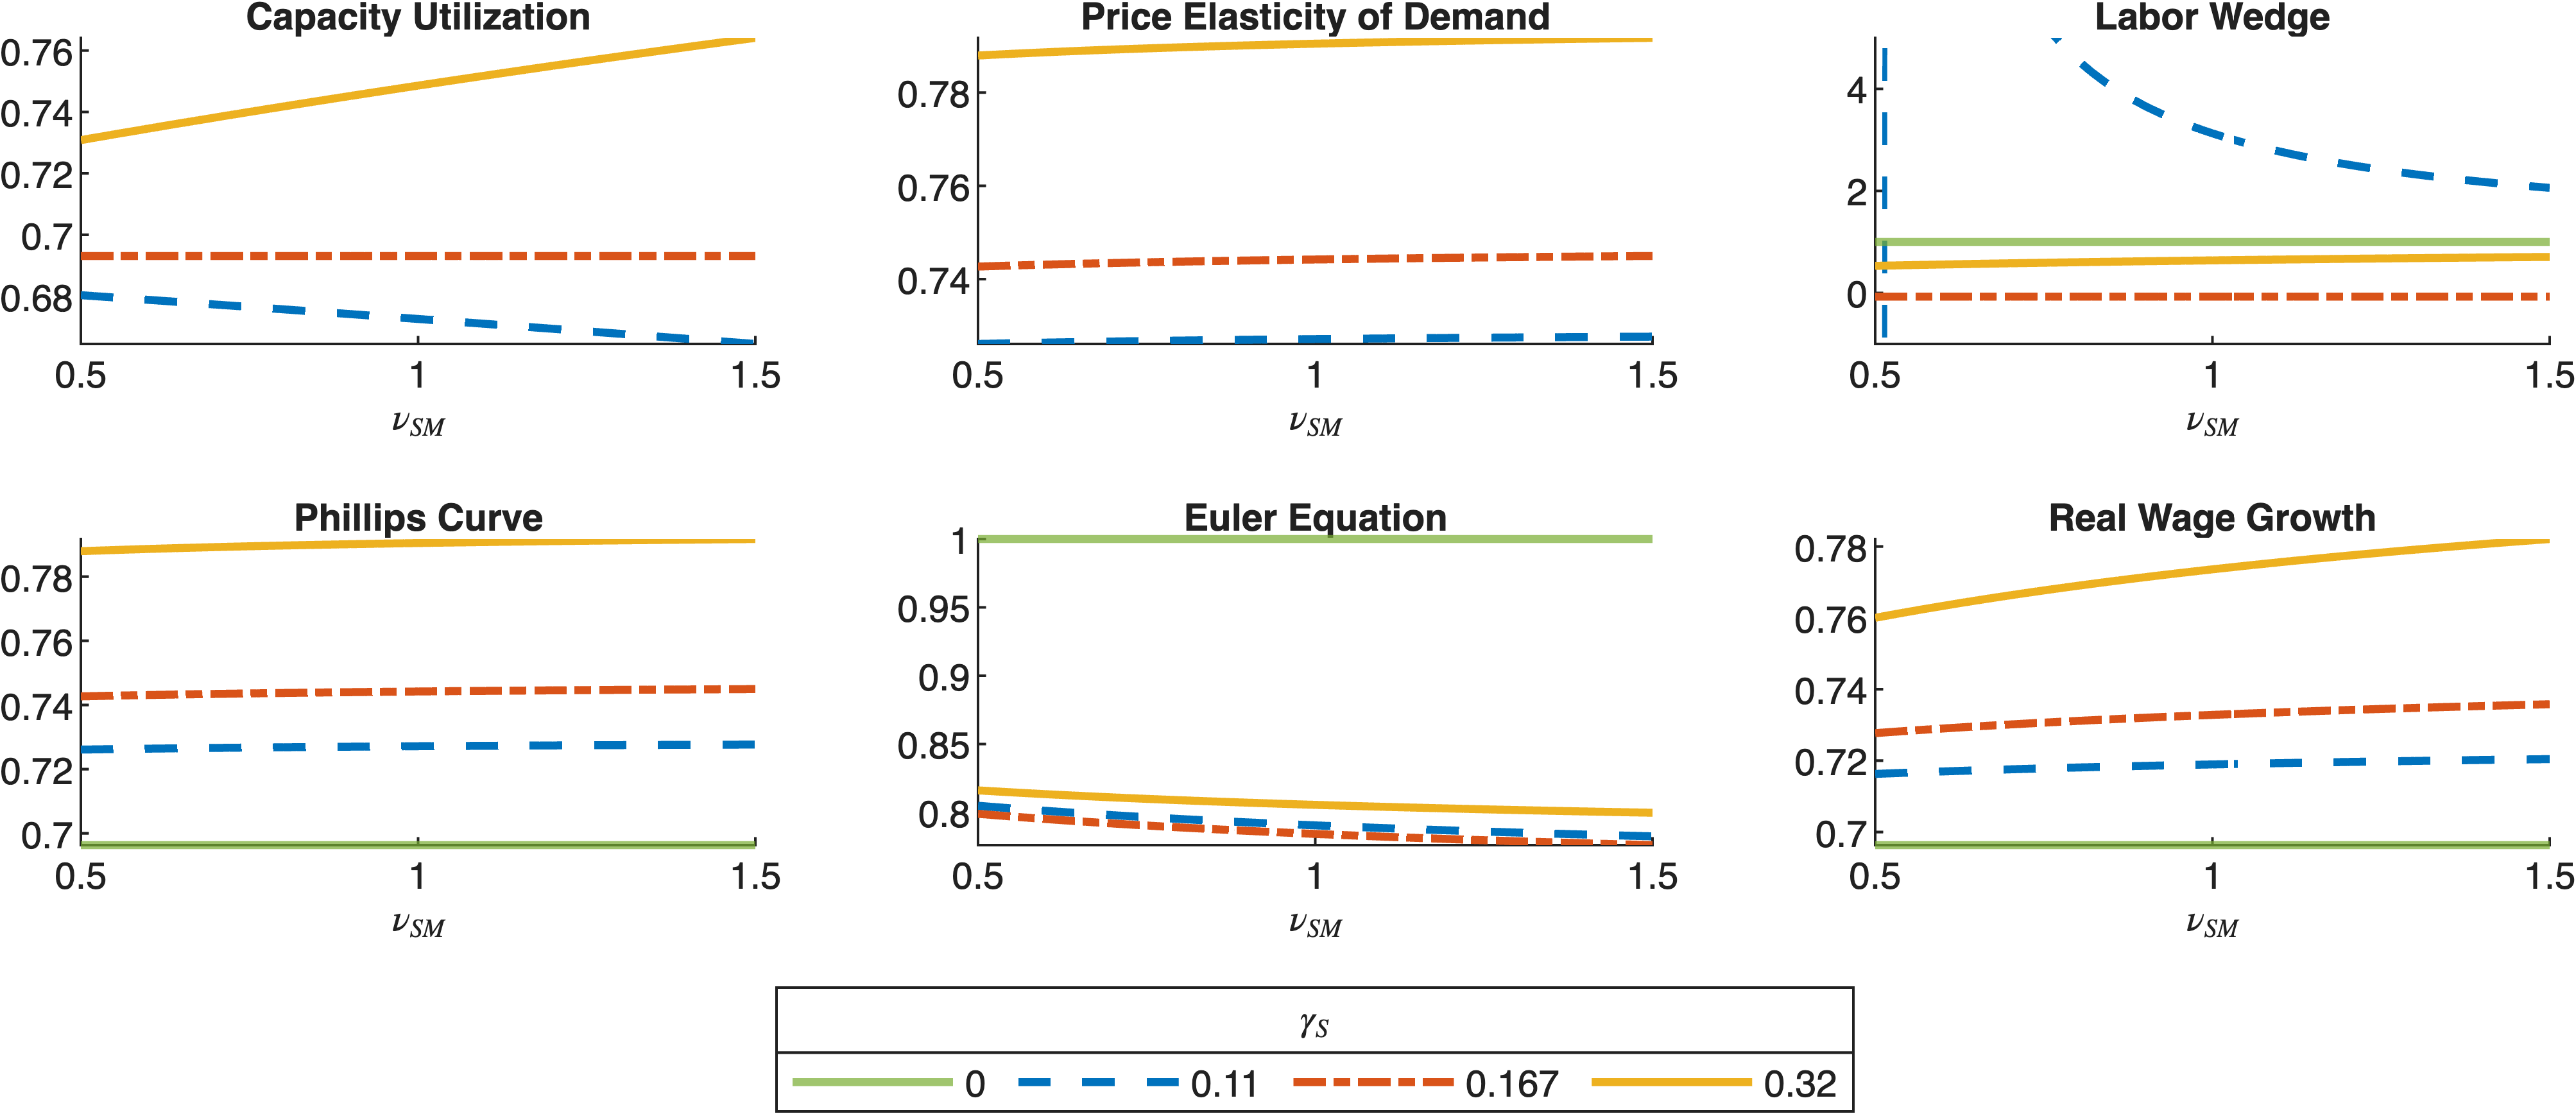
\includegraphics[width=\textwidth]{fig_28_slopes_robust_sw.png}\\%
    {\tiny \singlespacing NOTE: The graph shows the slopes of the NK-SaM model with sticky wages relative to without sticky wages. A value below one shows that the slope of a variable is smaller with sticky wages compared to a model with flexible wages. The figure shows how this ratio changes for different combinations of $\gamma_S$ and $\nu_{SM} = \nicefrac{\nu_S}{\nu_M}$.\par}%
\end{figure}%
% Statistics Table
\begin{table}[h!]%
	\begin{center}%
		\begin{footnotesize}%
			\caption{Flexible Wages - Relative Standard Deviations and Correlations}\label{tab:app_robust_sw}%
			\begin{tabular}{l r r r r r r r r}%
				\hline%
				& \multicolumn{2}{c}{TFP} & \multicolumn{2}{c}{Policy} & \multicolumn{2}{c}{Cost-Push} & \multicolumn{2}{c}{Search}\\%
				Variable & Rel.Std. & Corr. & Rel.Std. & Corr. & Rel.Std. & Corr. & Rel.Std. & Corr.\\%
				\hline \hline%
				Output Gap & 0.07 & -0.96 & 1.00 & 1.00 & 0.32 & -1.00 & 0.12 & -1.00\\%
				UE Gap & - & - & - & - & - & - & - & -\\%
				Inflation & 0.05 & -0.98 & 0.56 & 1.00 & 0.07 & -0.98 & 0.03 & -0.99\\%
				Real Wage & 0.71 & 0.99 & 5.22 & 1.00 & 3.71 & 1.00 & 0.46 & 1.00\\%
				Utilization & 0.55 & -1.00 & 1.97 & 1.00 & 0.63 & -1.00 & 0.7 & 1.00\\%
				Marginal Cost & 0.19 & -0.96 & 2.92 & 1.00 & 4.44 & 1.00 & 0.35 & -1.00\\%
				Price Elasticity & 0.45 & 0.96 & 6.88 & -1.00 & 29.06 & 1.00 & 0.83 & 1.00\\%
				Labor Wedge & 0.45 & 0.99 & 3.21 & 1.00 & 2.76 & -1.00 & 0.3 & 1.00\\%
				Search Effort & 0.36 & -0.95 & 5.87 & 1.00 & 0.57 & -0.97 & 2.73 & 1.00\\%
				\hline%
			\end{tabular}\\%
			\vspace{0.1in}%
			{\tiny NOTE: The table shows simulated second moments for the NK-SaM model. It shows relative standard deviations - standard deviation of each variable relative to standard deviation of real GDP - and correlations of each variable with real GDP. We consider each shock separately in the simulation.\par}%
		\end{footnotesize}%
	\end{center}%
\end{table}%
% IRF Figures - TFP AND DEMAND SHOCKS
\begin{figure}[h!]%
    \centering%
    \caption{Sticky and Flexible Wages - IRFs to Expansionary TFP and Demand Shocks}\label{fig:app_irf_robust_sw_1}%
    \begin{subfigure}{\textwidth}%
        \centering%
        \caption{IRFs to an Expansionary TFP Shock}%
        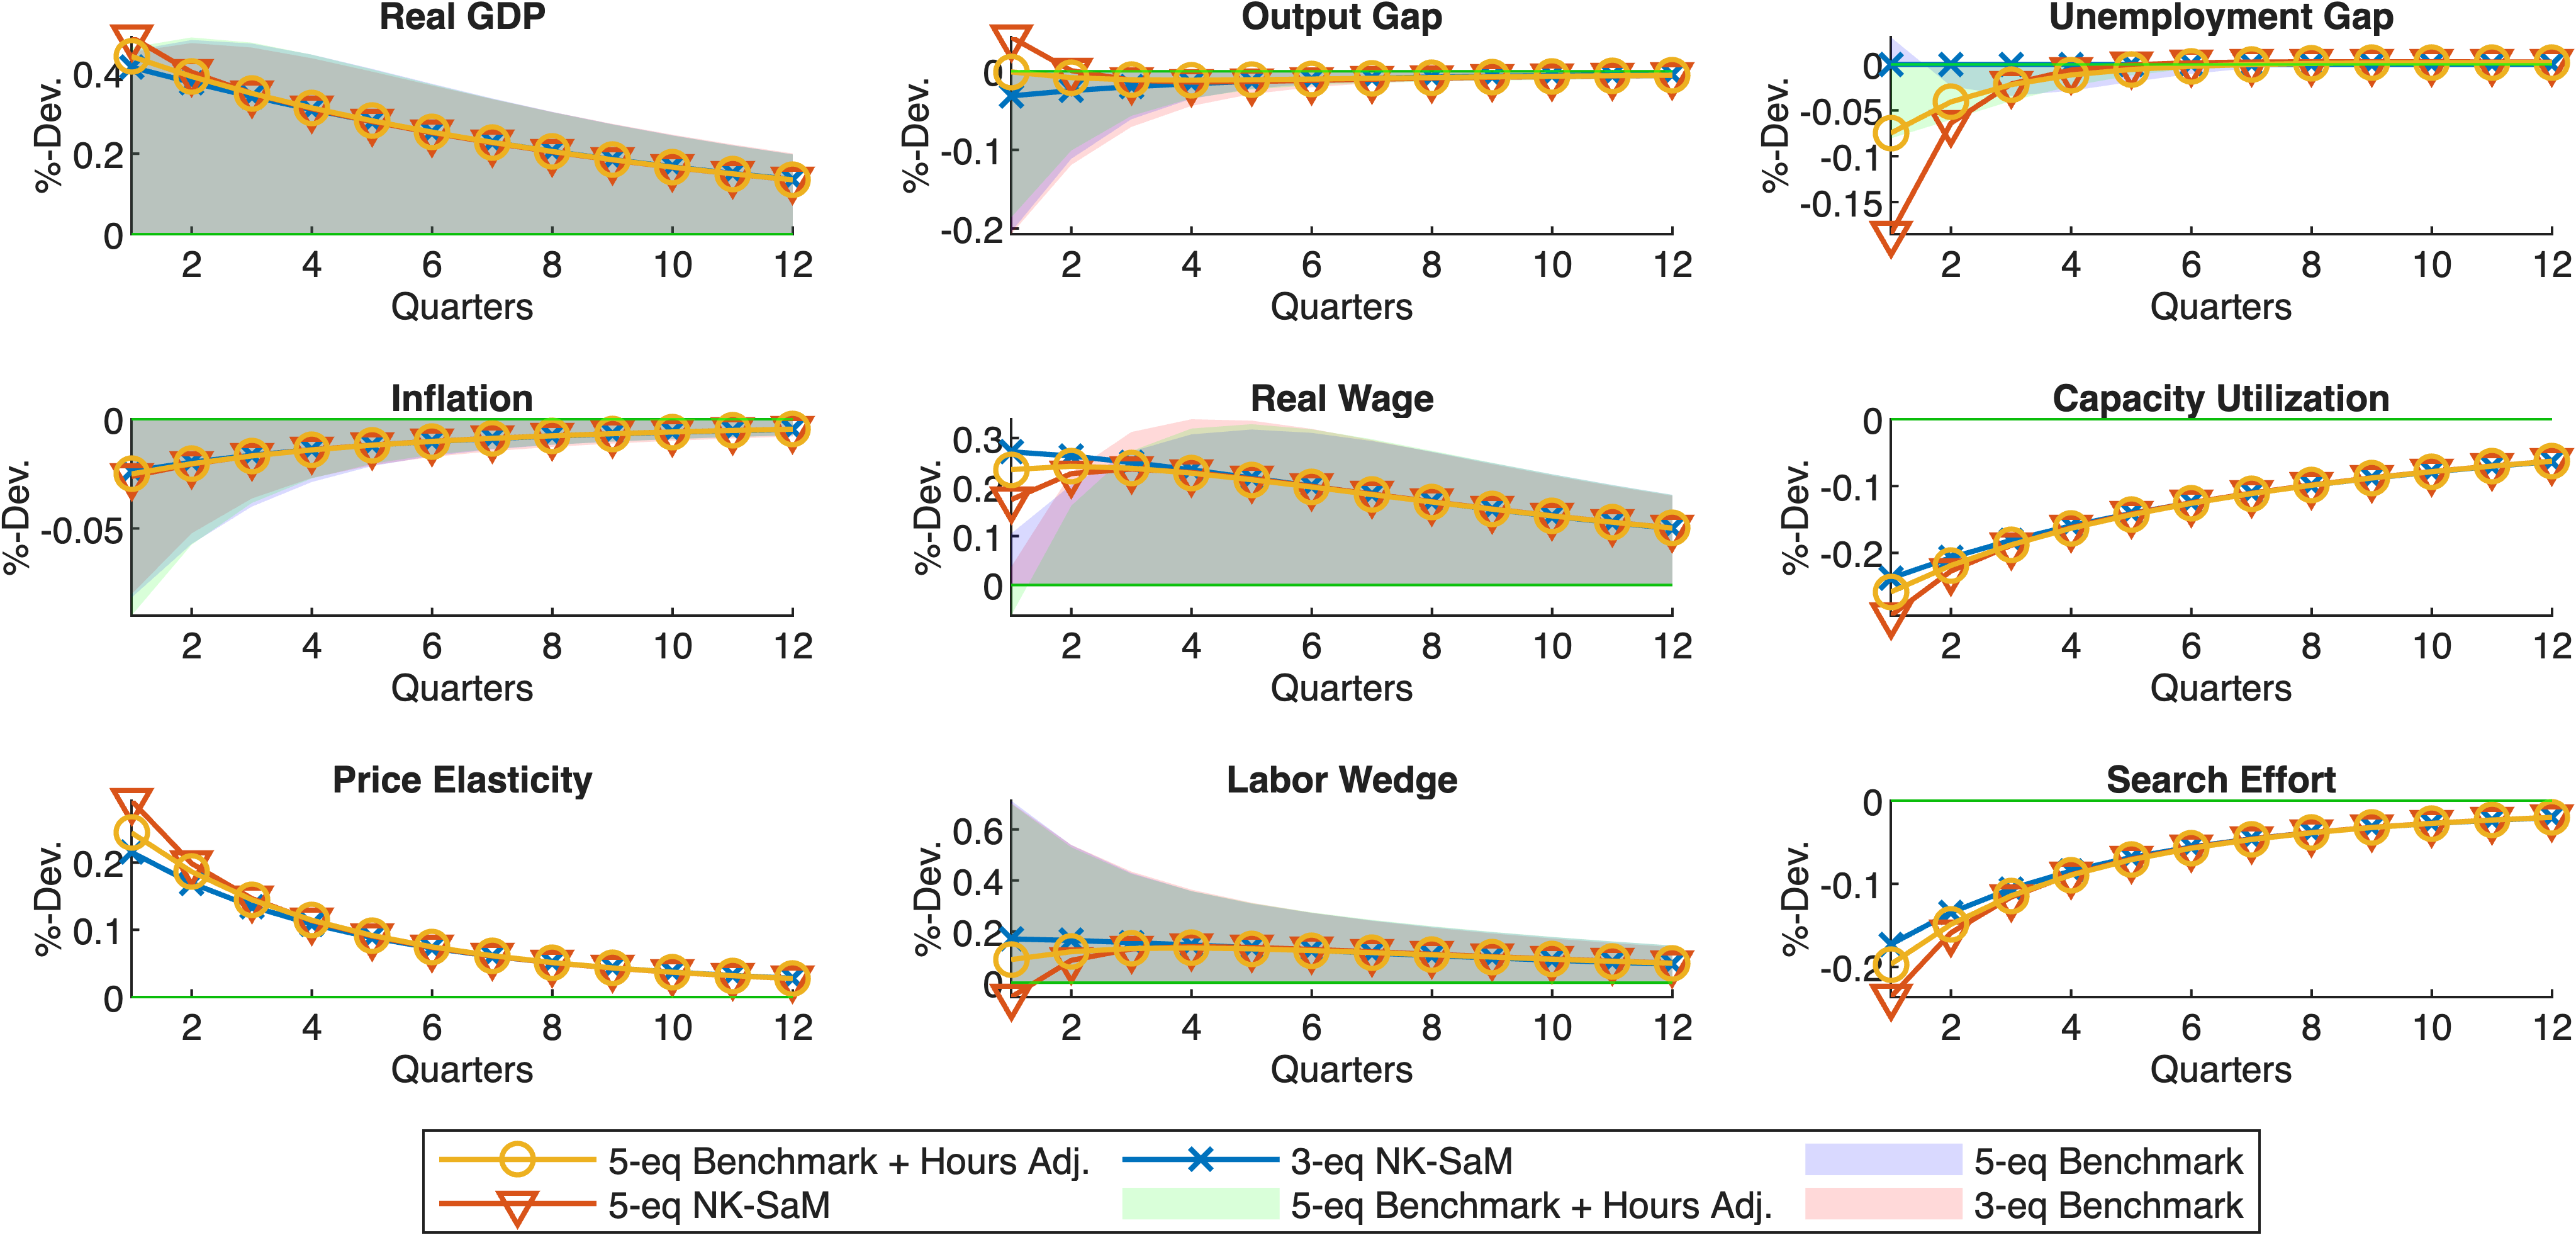
\includegraphics[width=\textwidth]{fig_29_irf_robust_stickywage_tfp.png}%
    \end{subfigure}\\%
	\vspace{0.2in}%
    \begin{subfigure}{\textwidth}%
        \centering%
        \caption{IRFs to an Expansionary Monetary Policy Shock}%
        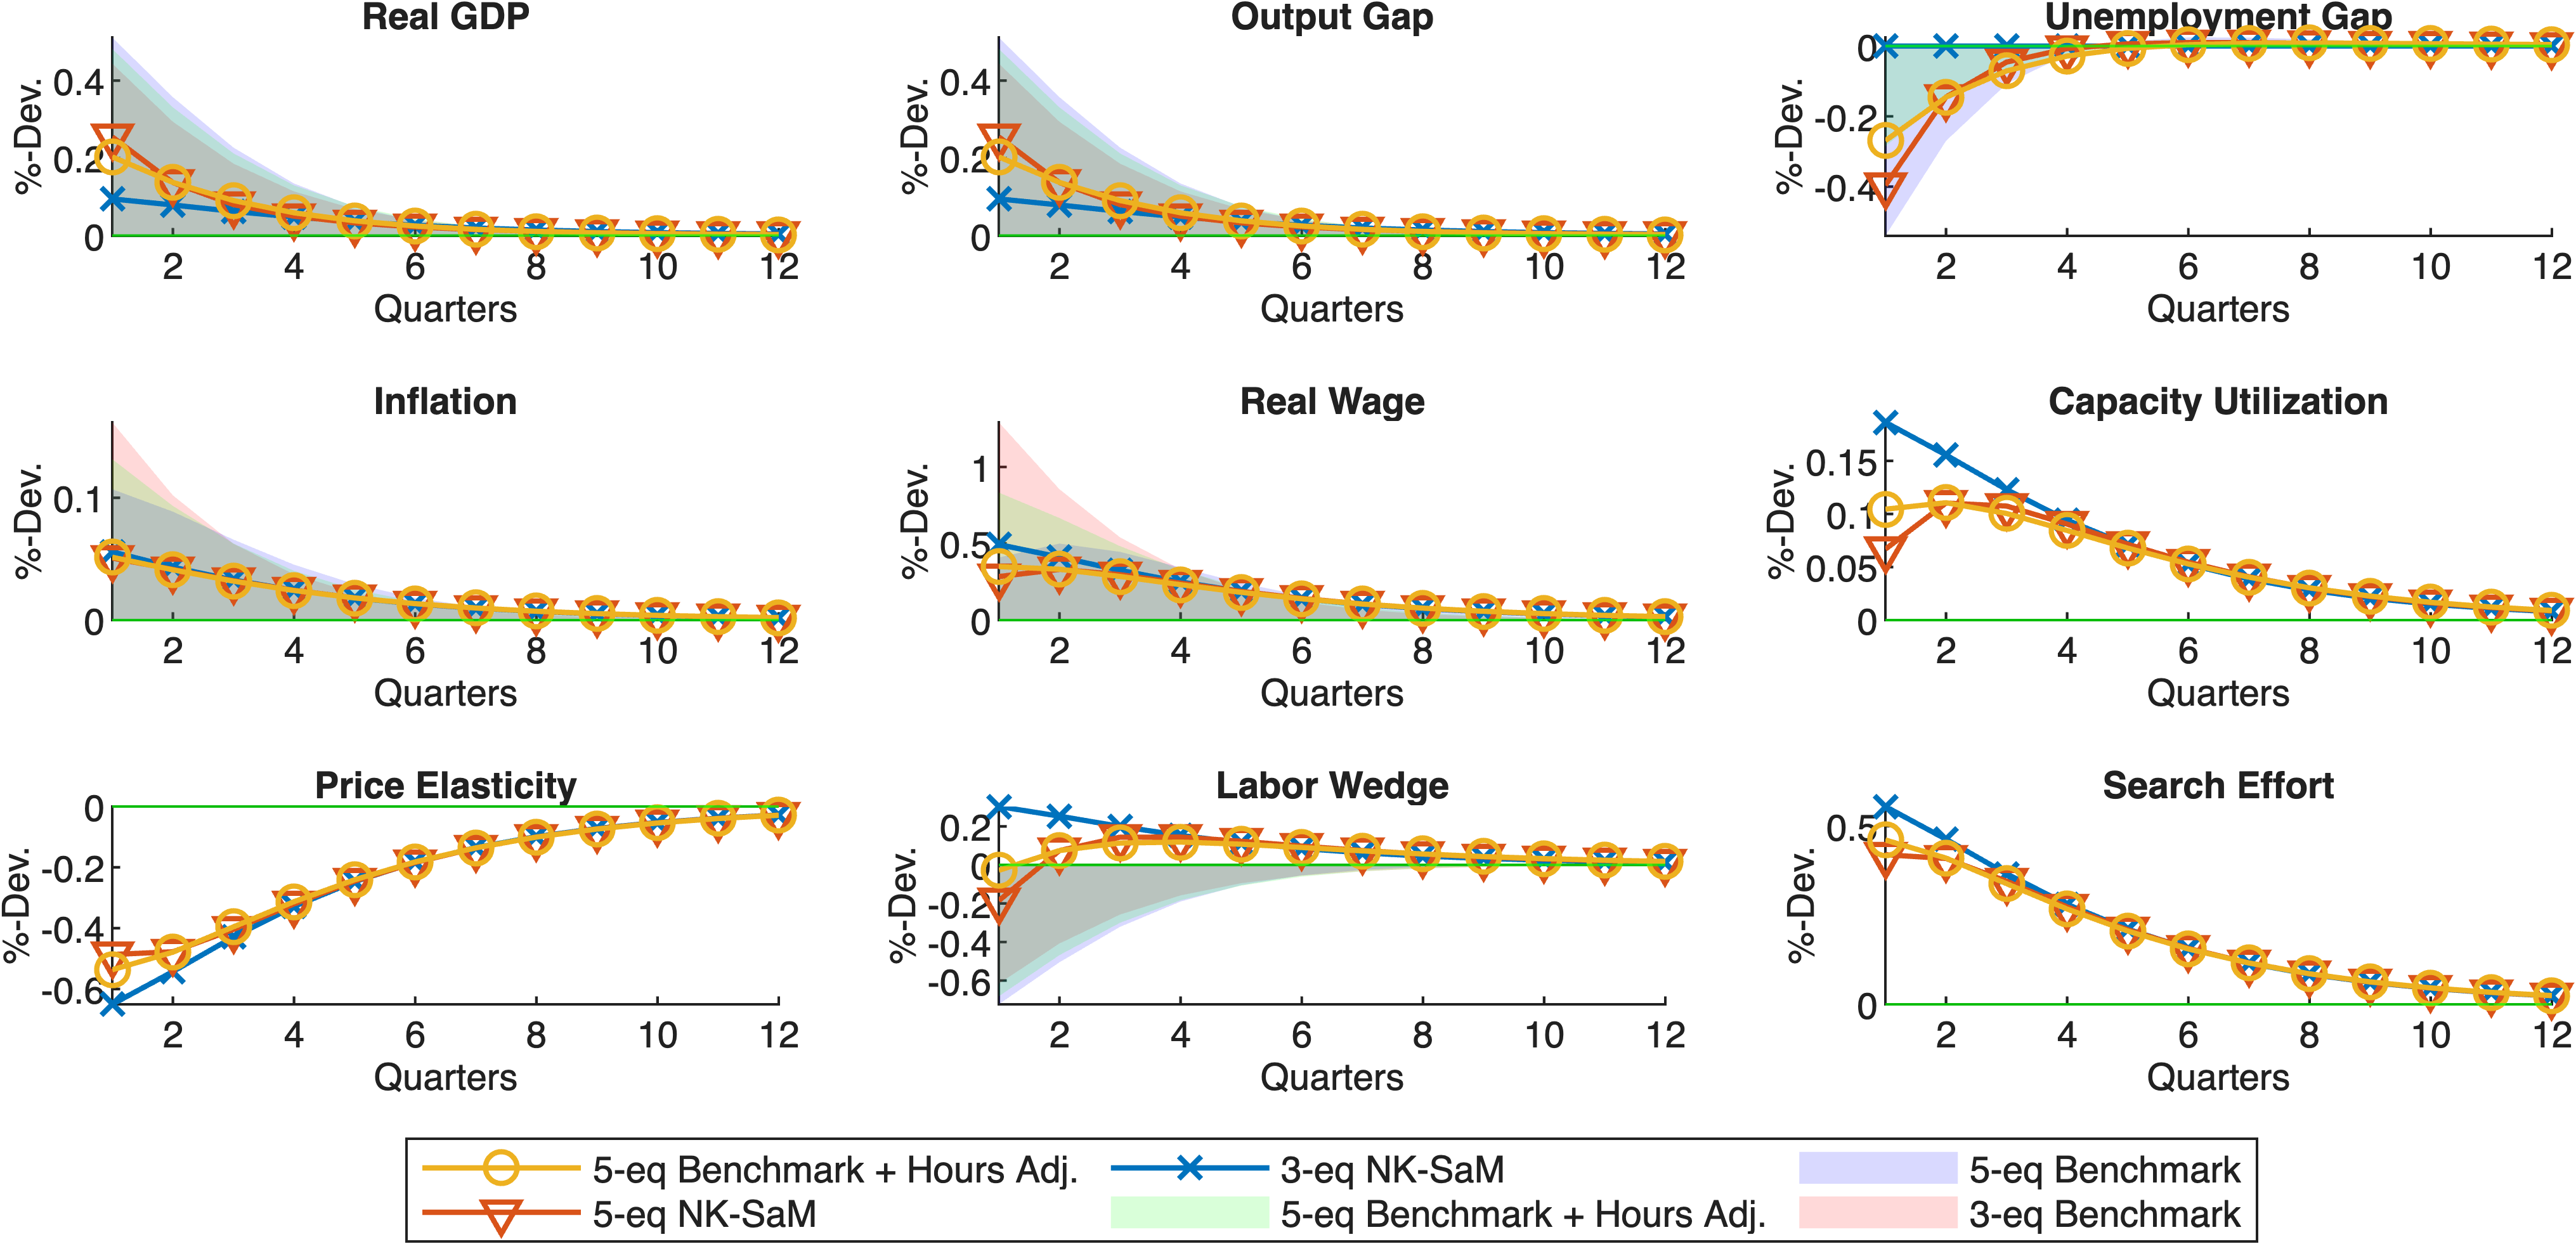
\includegraphics[width=\textwidth]{fig_30_irf_robust_stickywage_policy.png}%
    \end{subfigure}\\%
    {\tiny \singlespacing The figure shows IRFs to one standard deviation expansionary shocks using the model presented in \cref{sec:model} and \cref{sec:dynamics}. The benchmark model follows \cref{prop:nosam}, the 5-equation NK-SaM model is calibrated as in \cref{tab:calibration}. The 3-equation benchmark and NK-SaM models calibrate $\kappa_W=0$. For the ''hours adjustment costs'' addition, we calibrate $\kappa_{HM} = 4$. The model extension and its derivation is shown in \ref{sec:full_optimization}.\par}%
\end{figure}%
% IRF Figures - TFP AND DEMAND SHOCKS
\begin{figure}[h!]%
    \centering%
    \caption{Sticky and Flexible Wages - IRFs to Expansionary Cost Push Shocks}\label{fig:app_irf_robust_sw_2}%
    \begin{subfigure}{\textwidth}%
        \centering%
        \caption{IRFs to an Expansionary EIS Shock}%
        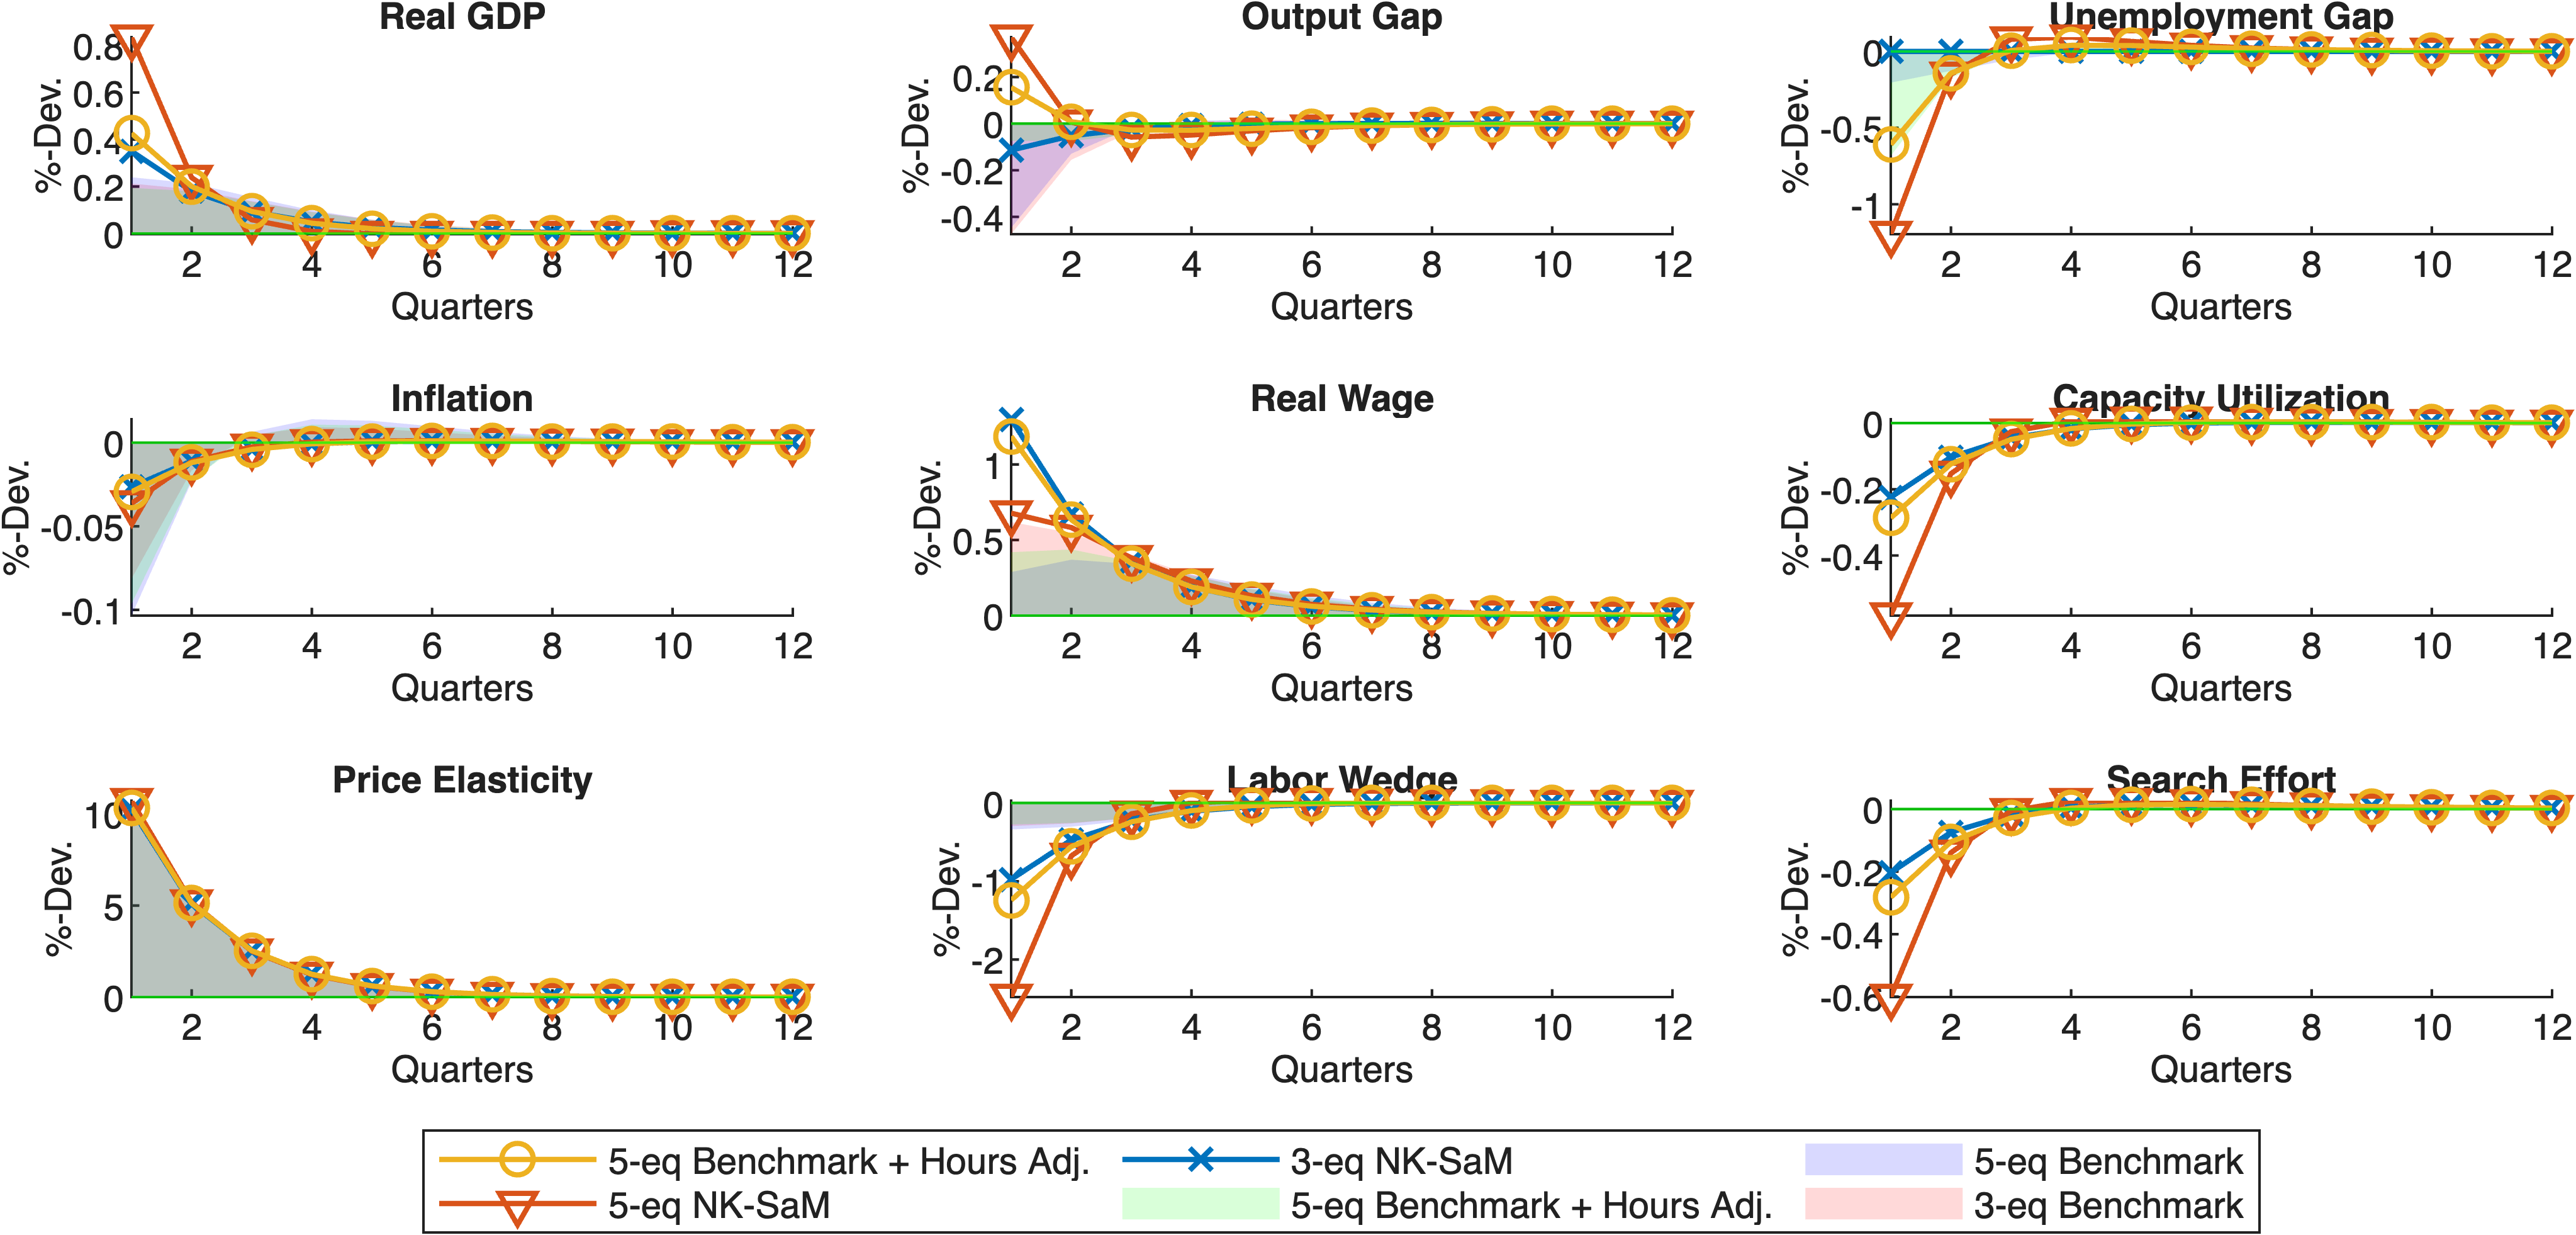
\includegraphics[width=\textwidth]{fig_31_irf_robust_stickywage_eis.png}%
    \end{subfigure}\\%
	\vspace{0.2in}%
    \begin{subfigure}{\textwidth}%
        \centering%
        \caption{IRFs to an Expansionary Search Effort Shock}%
        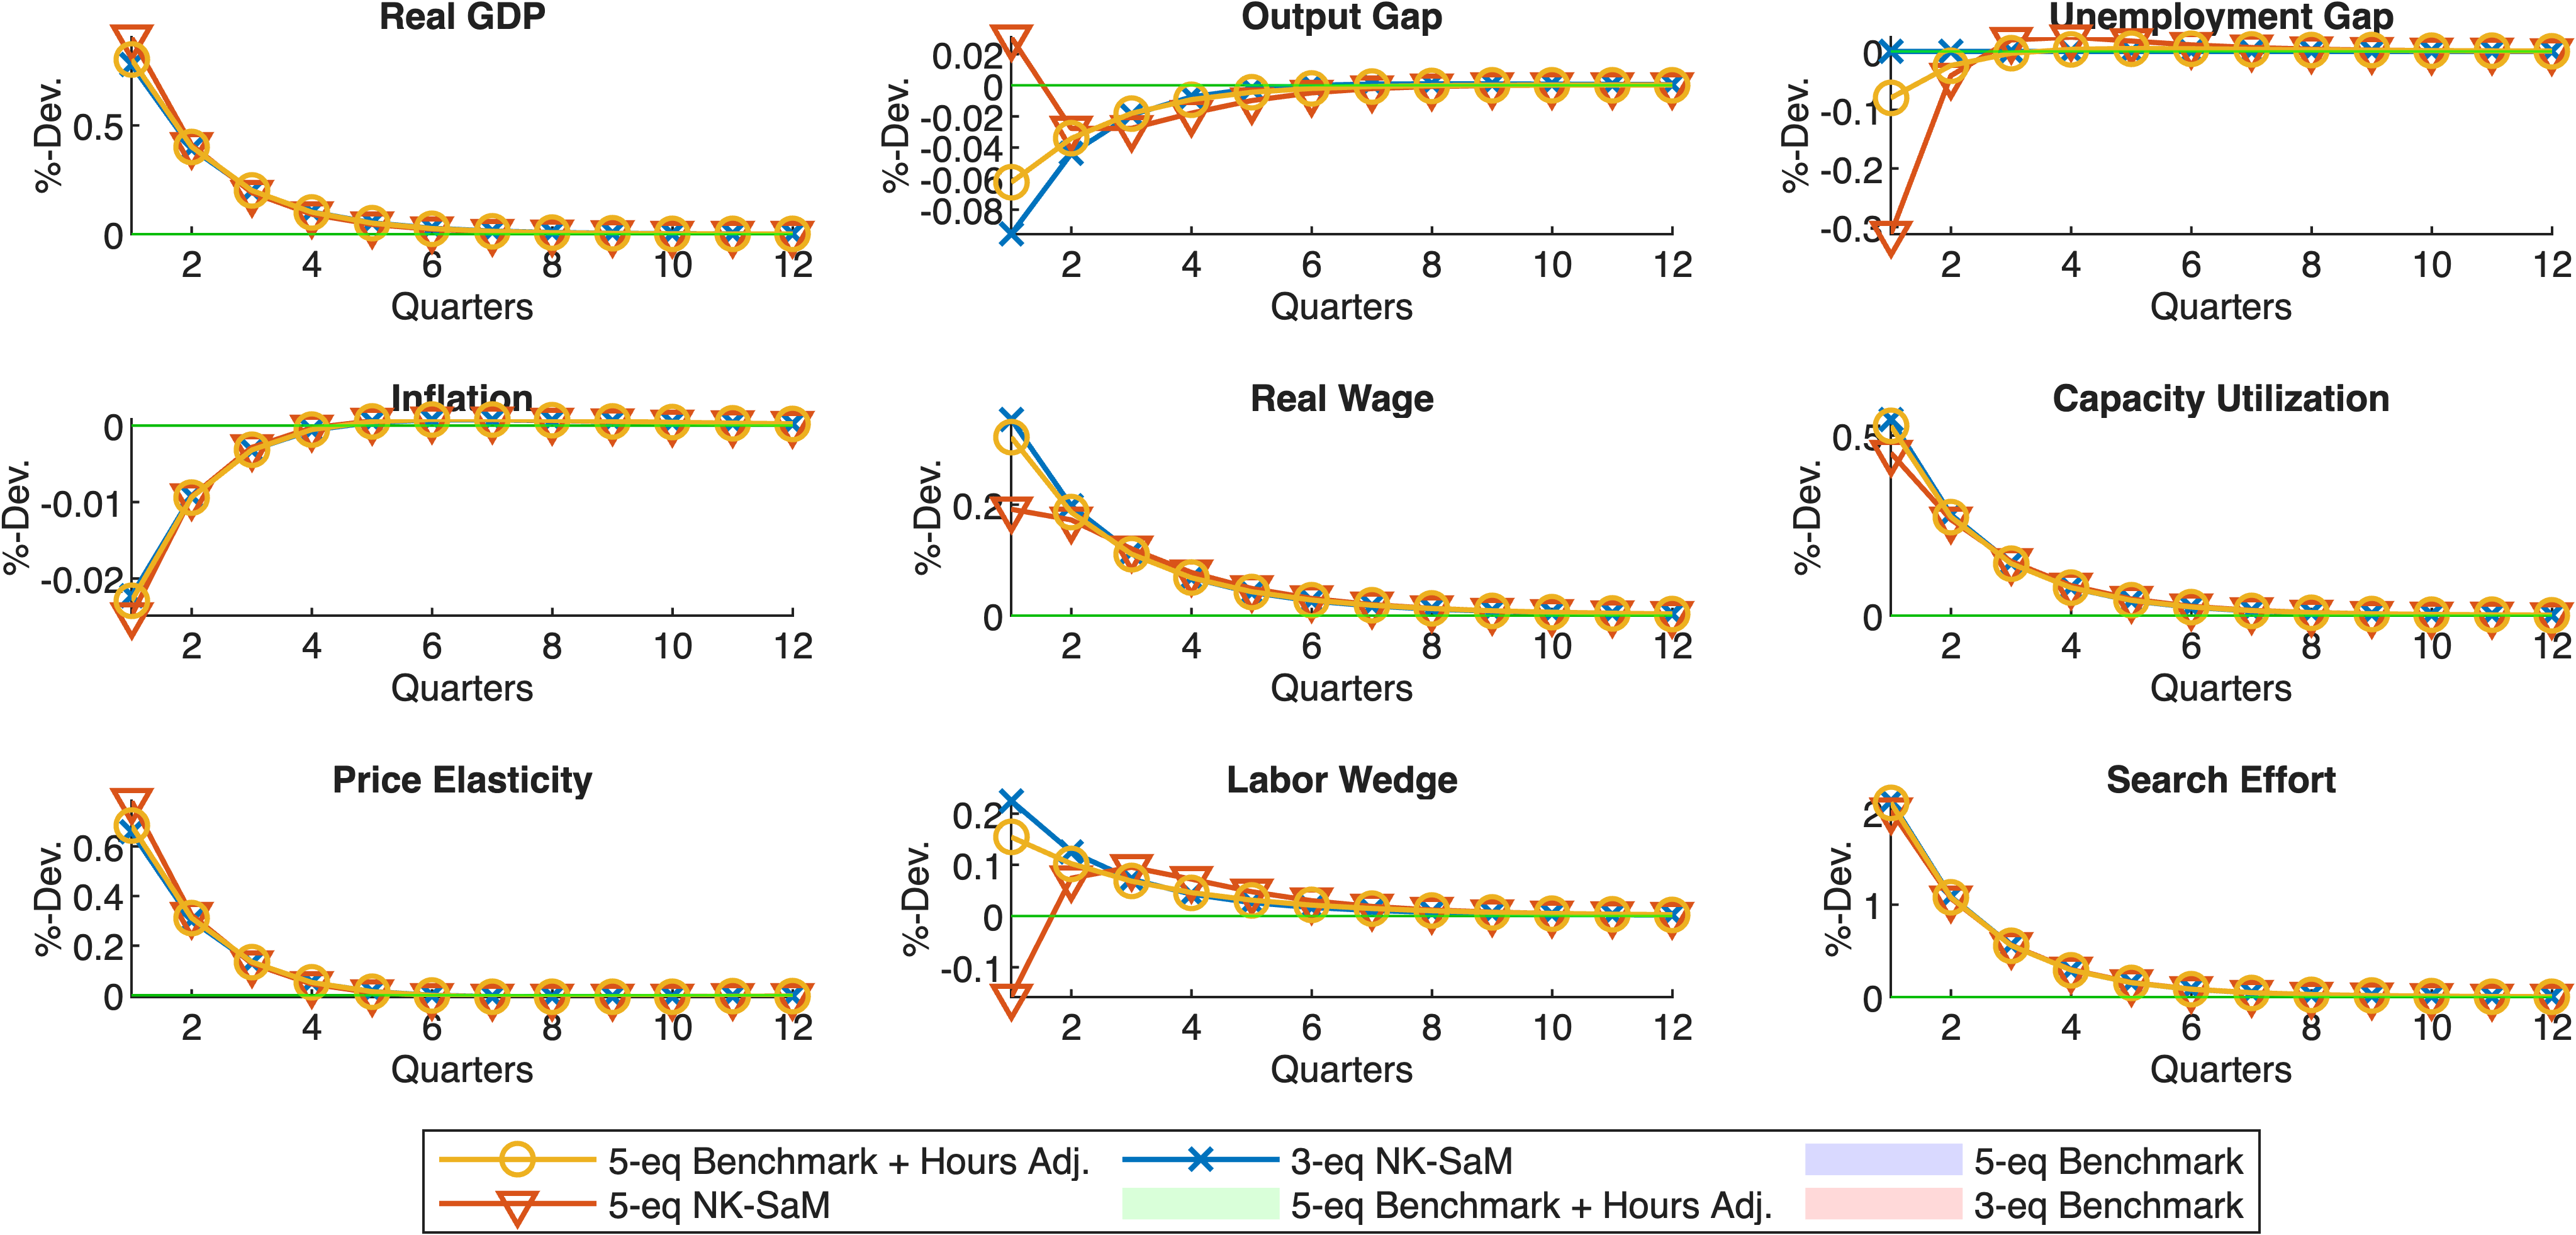
\includegraphics[width=\textwidth]{fig_32_irf_robust_stickywage_search.png}%
    \end{subfigure}\\%
    {\tiny \singlespacing The figure shows IRFs to one standard deviation expansionary shocks using the model presented in \cref{sec:model} and \cref{sec:dynamics}. The benchmark model follows \cref{prop:nosam}, the 5-equation NK-SaM model is calibrated as in \cref{tab:calibration}. The 3-equation benchmark and NK-SaM models calibrate $\kappa_W=0$. For the ''hours adjustment costs'' addition, we calibrate $\kappa_{HM} = 4$. The model extension and its derivation is shown in \ref{sec:full_optimization}.\par}%
\end{figure}%
% ROBUSTNESS: CAPITAL AND CAPITAL UTILIZATION
%-----------------------------------------------------------
\FloatBarrier%
\pagebreak%
\subsection{Robustness - Capital and Capital Utilization}\label{sec:robust_capital}%
% Statistics Table
%--------------------------------------------------------------------------
\begin{table}[h!]%
	\begin{center}%
		\begin{footnotesize}%
			\caption{Adding Capital (Utilization) - Relative Standard Deviations and Correlations}\label{tab:app_robust_capital}%
			\begin{tabular}{l r r r r r r r r}%
				\hline%
				& \multicolumn{2}{c}{TFP} & \multicolumn{2}{c}{Policy} & \multicolumn{2}{c}{Cost-Push} & \multicolumn{2}{c}{Search}\\%
				Variable & Rel.Std. & Corr. & Rel.Std. & Corr. & Rel.Std. & Corr. & Rel.Std. & Corr.\\%
				\hline \hline%
				Output Gap & 0.03 & -0.01 & 1.00 & 1.00 & 0.32 & 0.91 & 0.02 & -0.30\\%
				UE Gap & 0.20 & -0.63 & 1.87 & -0.93 & 1.41 & -0.95 & 0.28 & -0.91\\%
				Inflation & 0.03 & -0.77 & 0.35 & 0.97 & 0.05 & -0.98 & 0.03 & -0.90\\%
				Real Wage & 0.59 & 0.94 & 2.41 & 0.85 & 1.12 & 0.87 & 0.30 & 0.87\\%
				Utilization & 0.44 & -0.91 & 0.69 & 0.80 & 0.36 & -0.91 & 0.63 & 1.00\\%
				Marginal Cost & 0.23 & -0.78 & 1.65 & 0.93 & 1.80 & 0.98 & 0.41 & -0.97\\%
				Price Elasticity & 0.54 & 0.78 & 3.88 & -0.93 & 14.12 & 0.99 & 0.95 & 0.97\\%
				Labor Wedge & 0.06 & 0.29 & 0.64 & -0.05 & 1.51 & -0.99 & 0.07 & -0.68\\%
				Search Effort & 0.47 & -0.54 & 3.34 & 0.92 & 0.87 & -0.96 & 2.35 & 1.00\\%
				\hline%
			\end{tabular}\\%
			\vspace{0.1in}%
			{\tiny NOTE: The table shows simulated second moments for the NK-SaM model. It shows relative standard deviations - standard deviation of each variable relative to standard deviation of real GDP - and correlations of each variable with real GDP. We consider each shock separately in the simulation.\par}%
		\end{footnotesize}%
	\end{center}%
\end{table}%
% IRF Figures - TFP AND DEMAND SHOCKS
\begin{figure}%
    \centering%
    \caption{Adding Capital (Utilization) - IRFs to Expansionary TFP and Demand Shocks}\label{fig:app_irf_robust_capital_1}%
    \begin{subfigure}{\textwidth}%
        \centering%
        \caption{IRFs to an Expansionary TFP Shock}%
        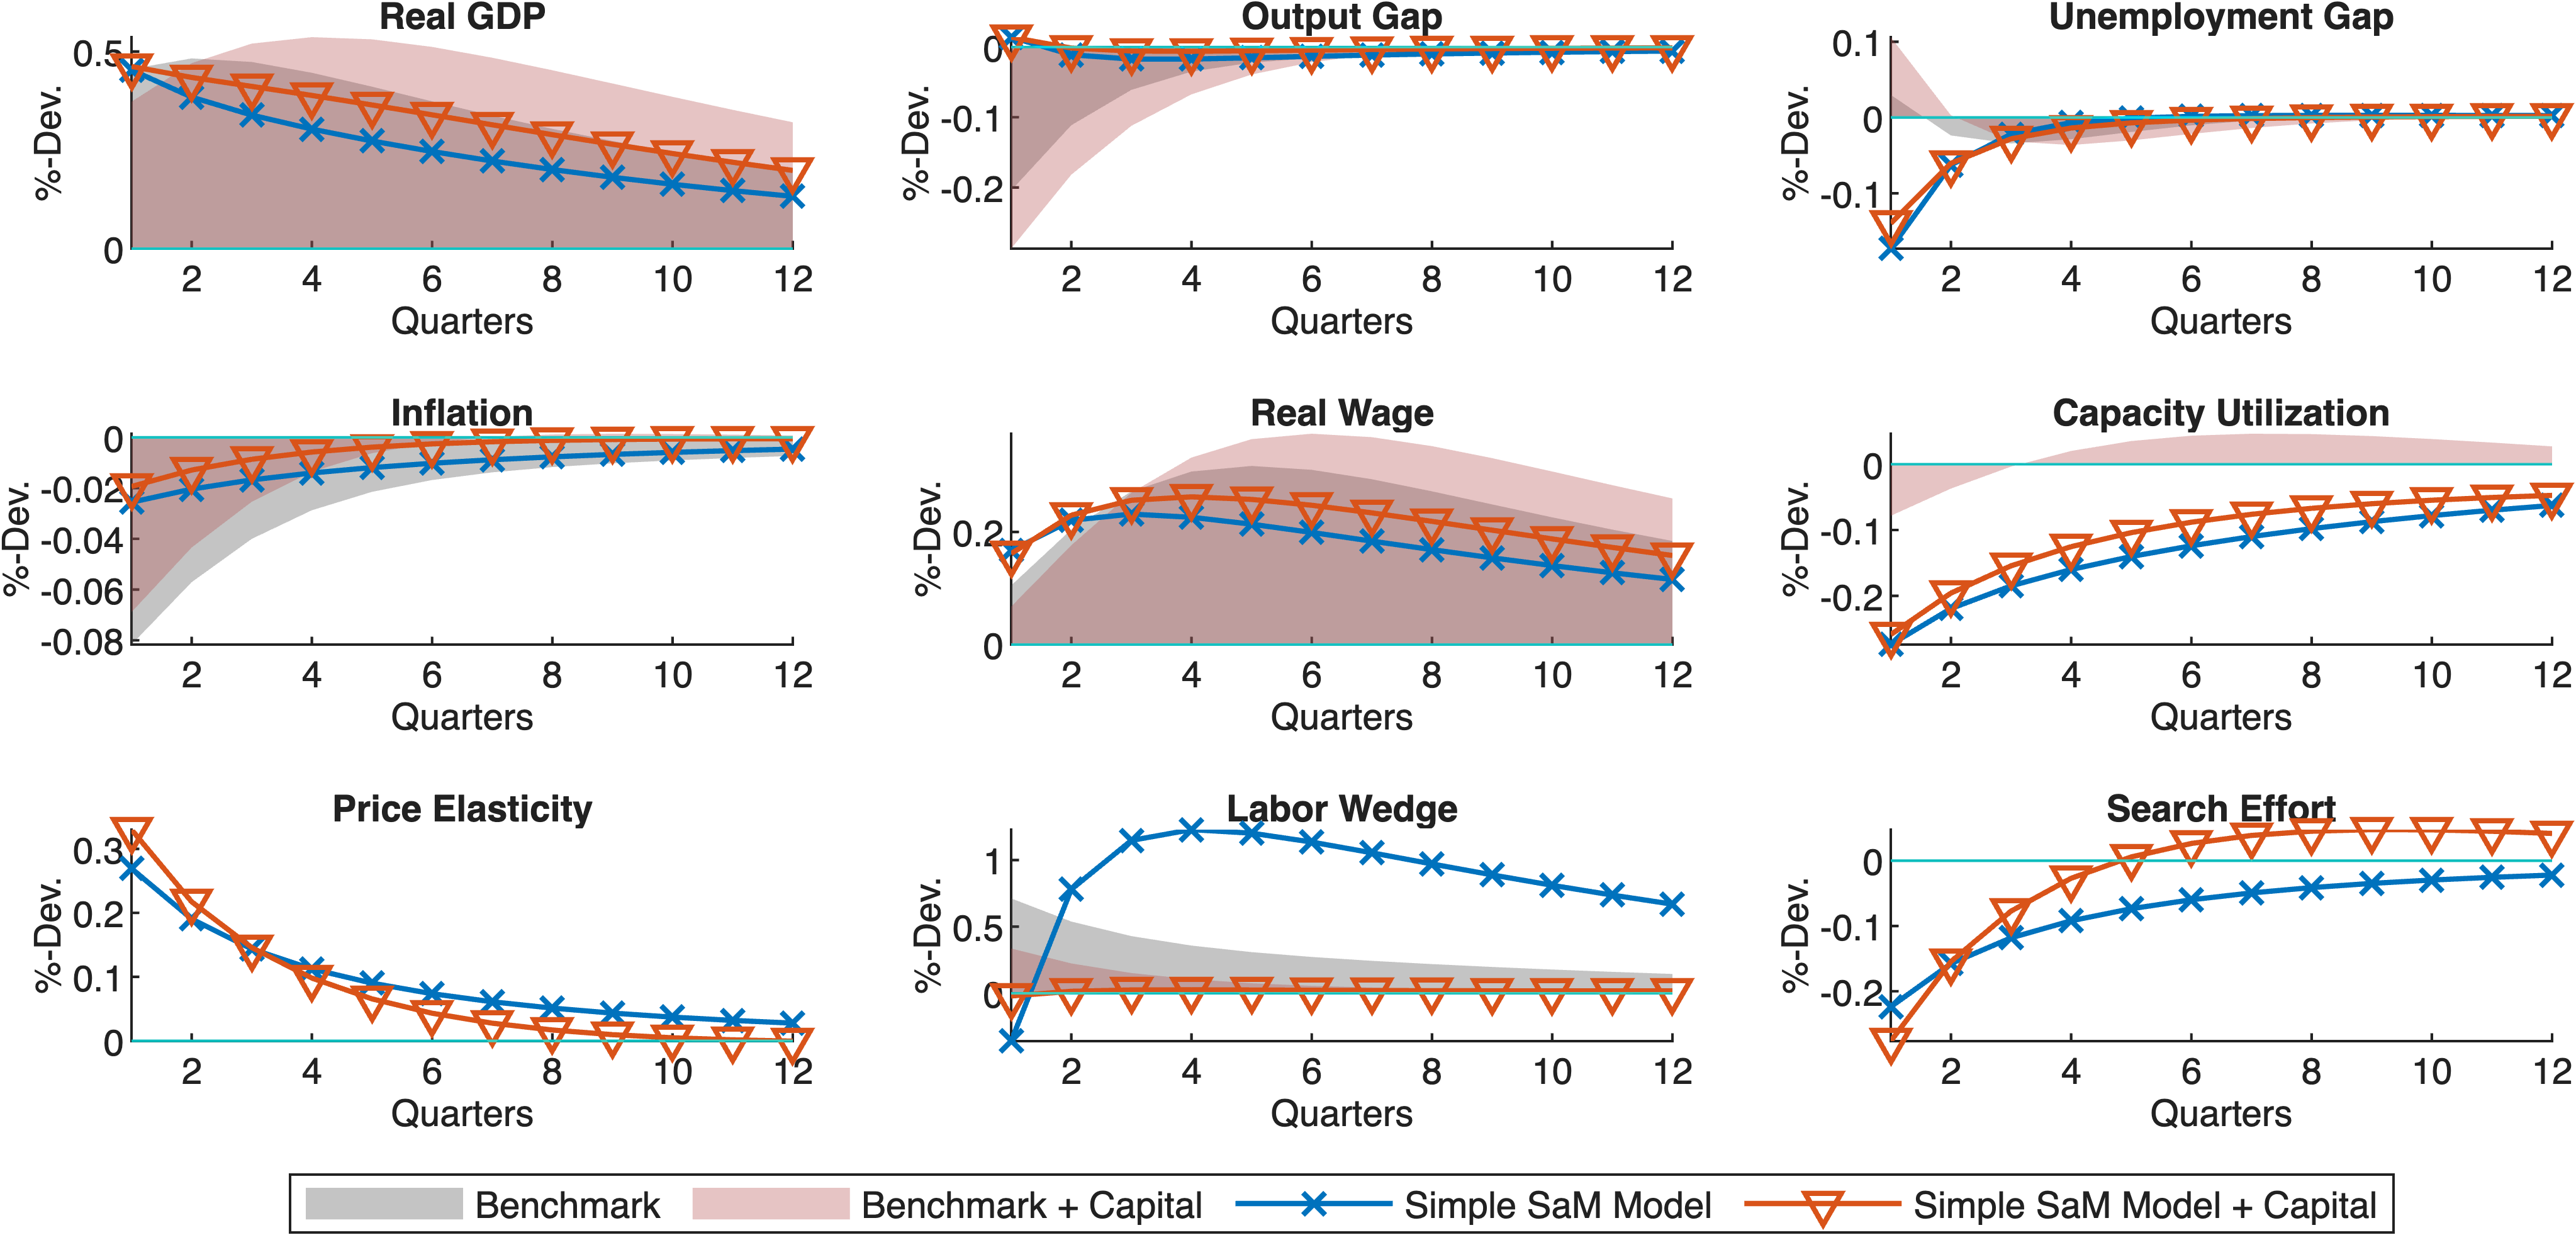
\includegraphics[width=\textwidth]{fig_33_irf_robust_capital_tfp.png}%
    \end{subfigure}\\%
	\vspace{0.2in}%
    \begin{subfigure}{\textwidth}%
        \centering%
        \caption{IRFs to an Expansionary Monetary Policy Shock}%
        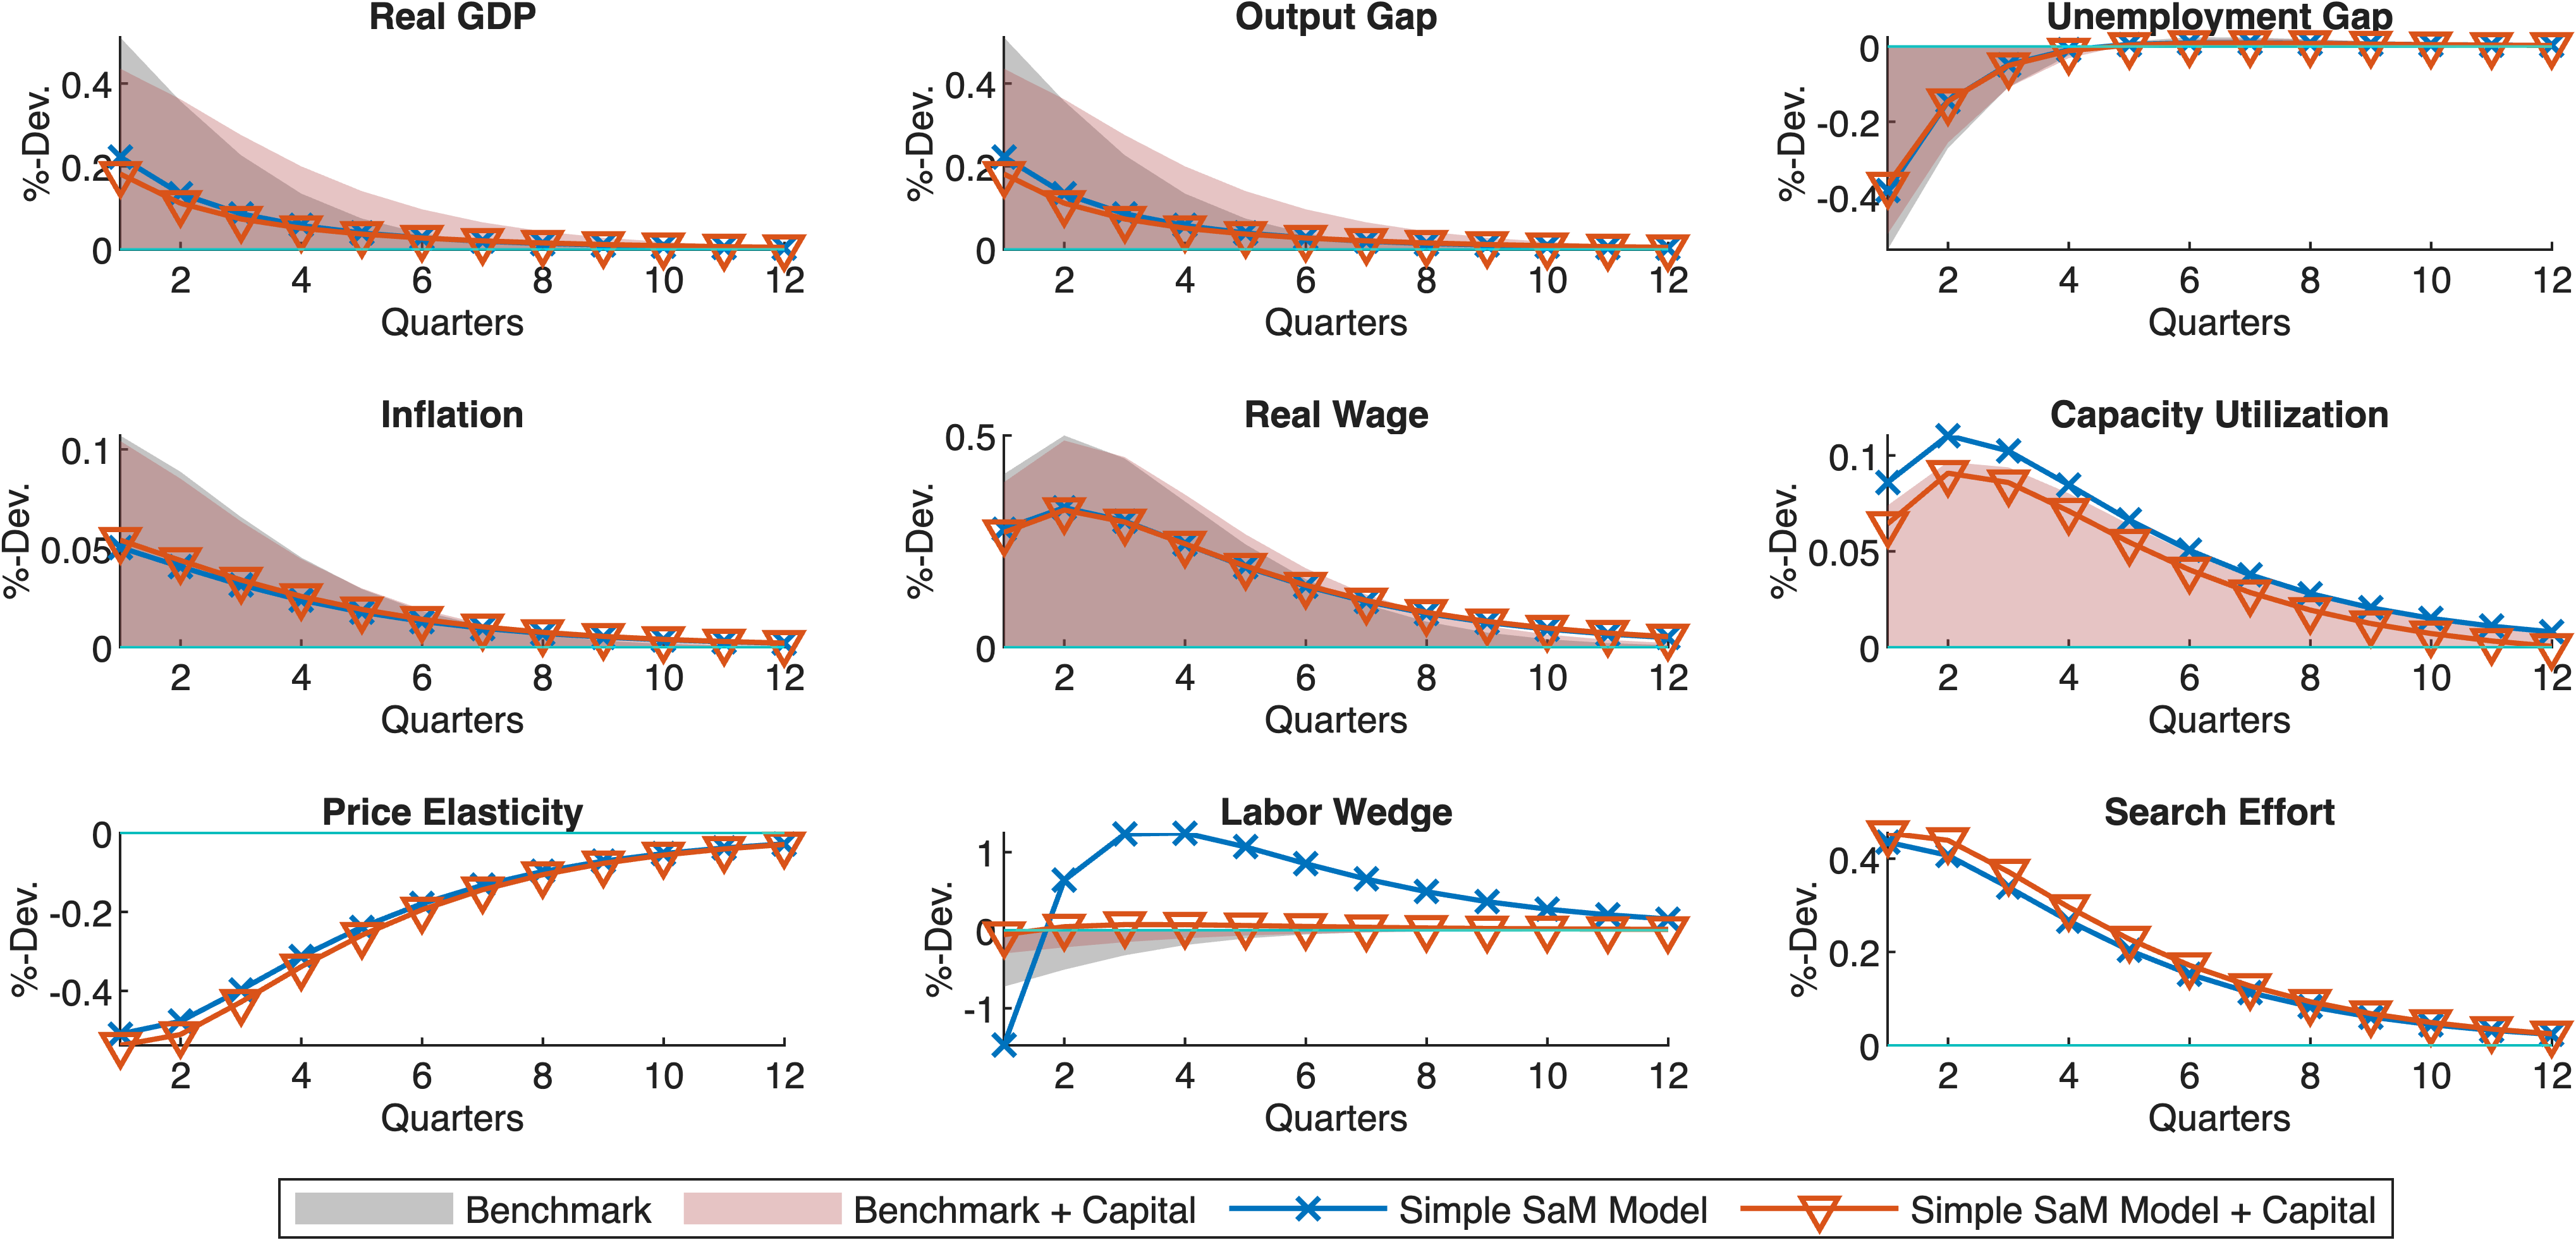
\includegraphics[width=\textwidth]{fig_34_irf_robust_capital_policy.png}%
    \end{subfigure}\\%
    {\tiny \singlespacing NOTE: The figure shows IRFs to one standard deviation expansionary shocks using the model presented in \cref{sec:model} and \cref{sec:dynamics}. The benchmark model follows \cref{prop:nosam}, the NK-SaM model is calibrated as in \cref{tab:calibration}. The capital stock and capital utilization channels are added as shown in \ref{sec:full_optimization} and calibrated as in \ref{sec:appendix_calibration}.\par}%
\end{figure}%
% IRF Figures - COST PUSH SHOCKS
\begin{figure}%
    \centering%
    \caption{Adding Capital (Utilization) - IRFs to Expansionary Cost Push Shocks}\label{fig:app_irf_robust_capital_2}%
    \begin{subfigure}{\textwidth}%
        \centering%
        \caption{IRFs to an Expansionary EIS Shock}%
        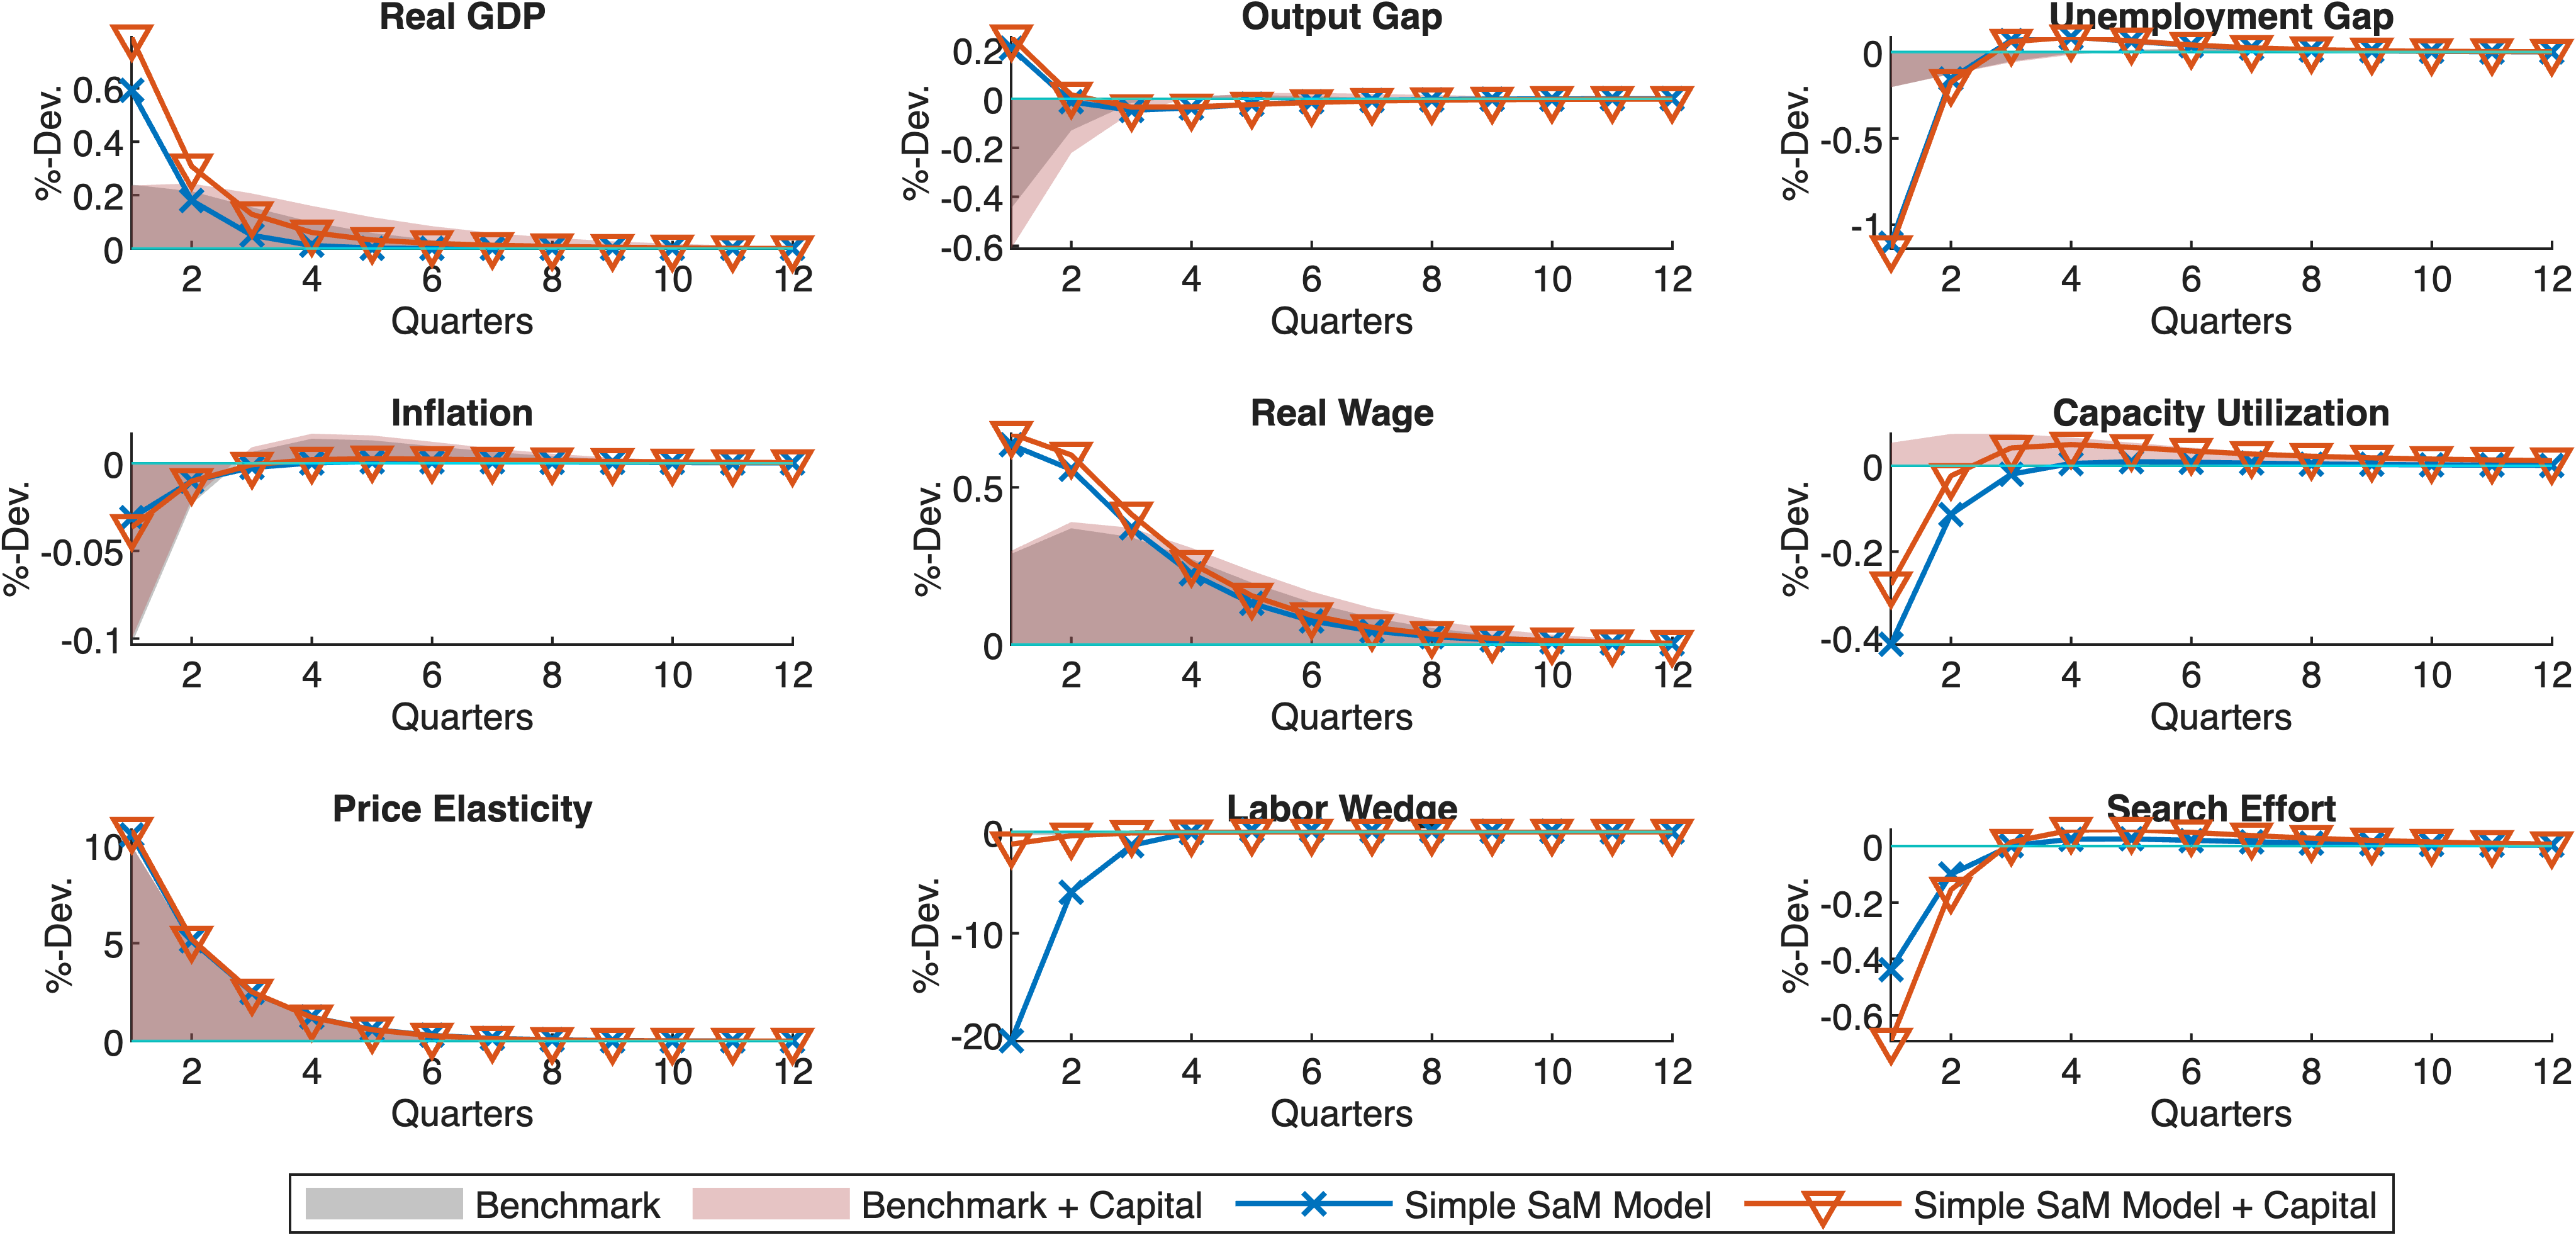
\includegraphics[width=\textwidth]{fig_35_irf_robust_capital_eis.png}%
    \end{subfigure}\\%
	\vspace{0.2in}%
    \begin{subfigure}{\textwidth}%
        \centering%
        \caption{IRFs to an Expansionary Search Effort Shock}%
        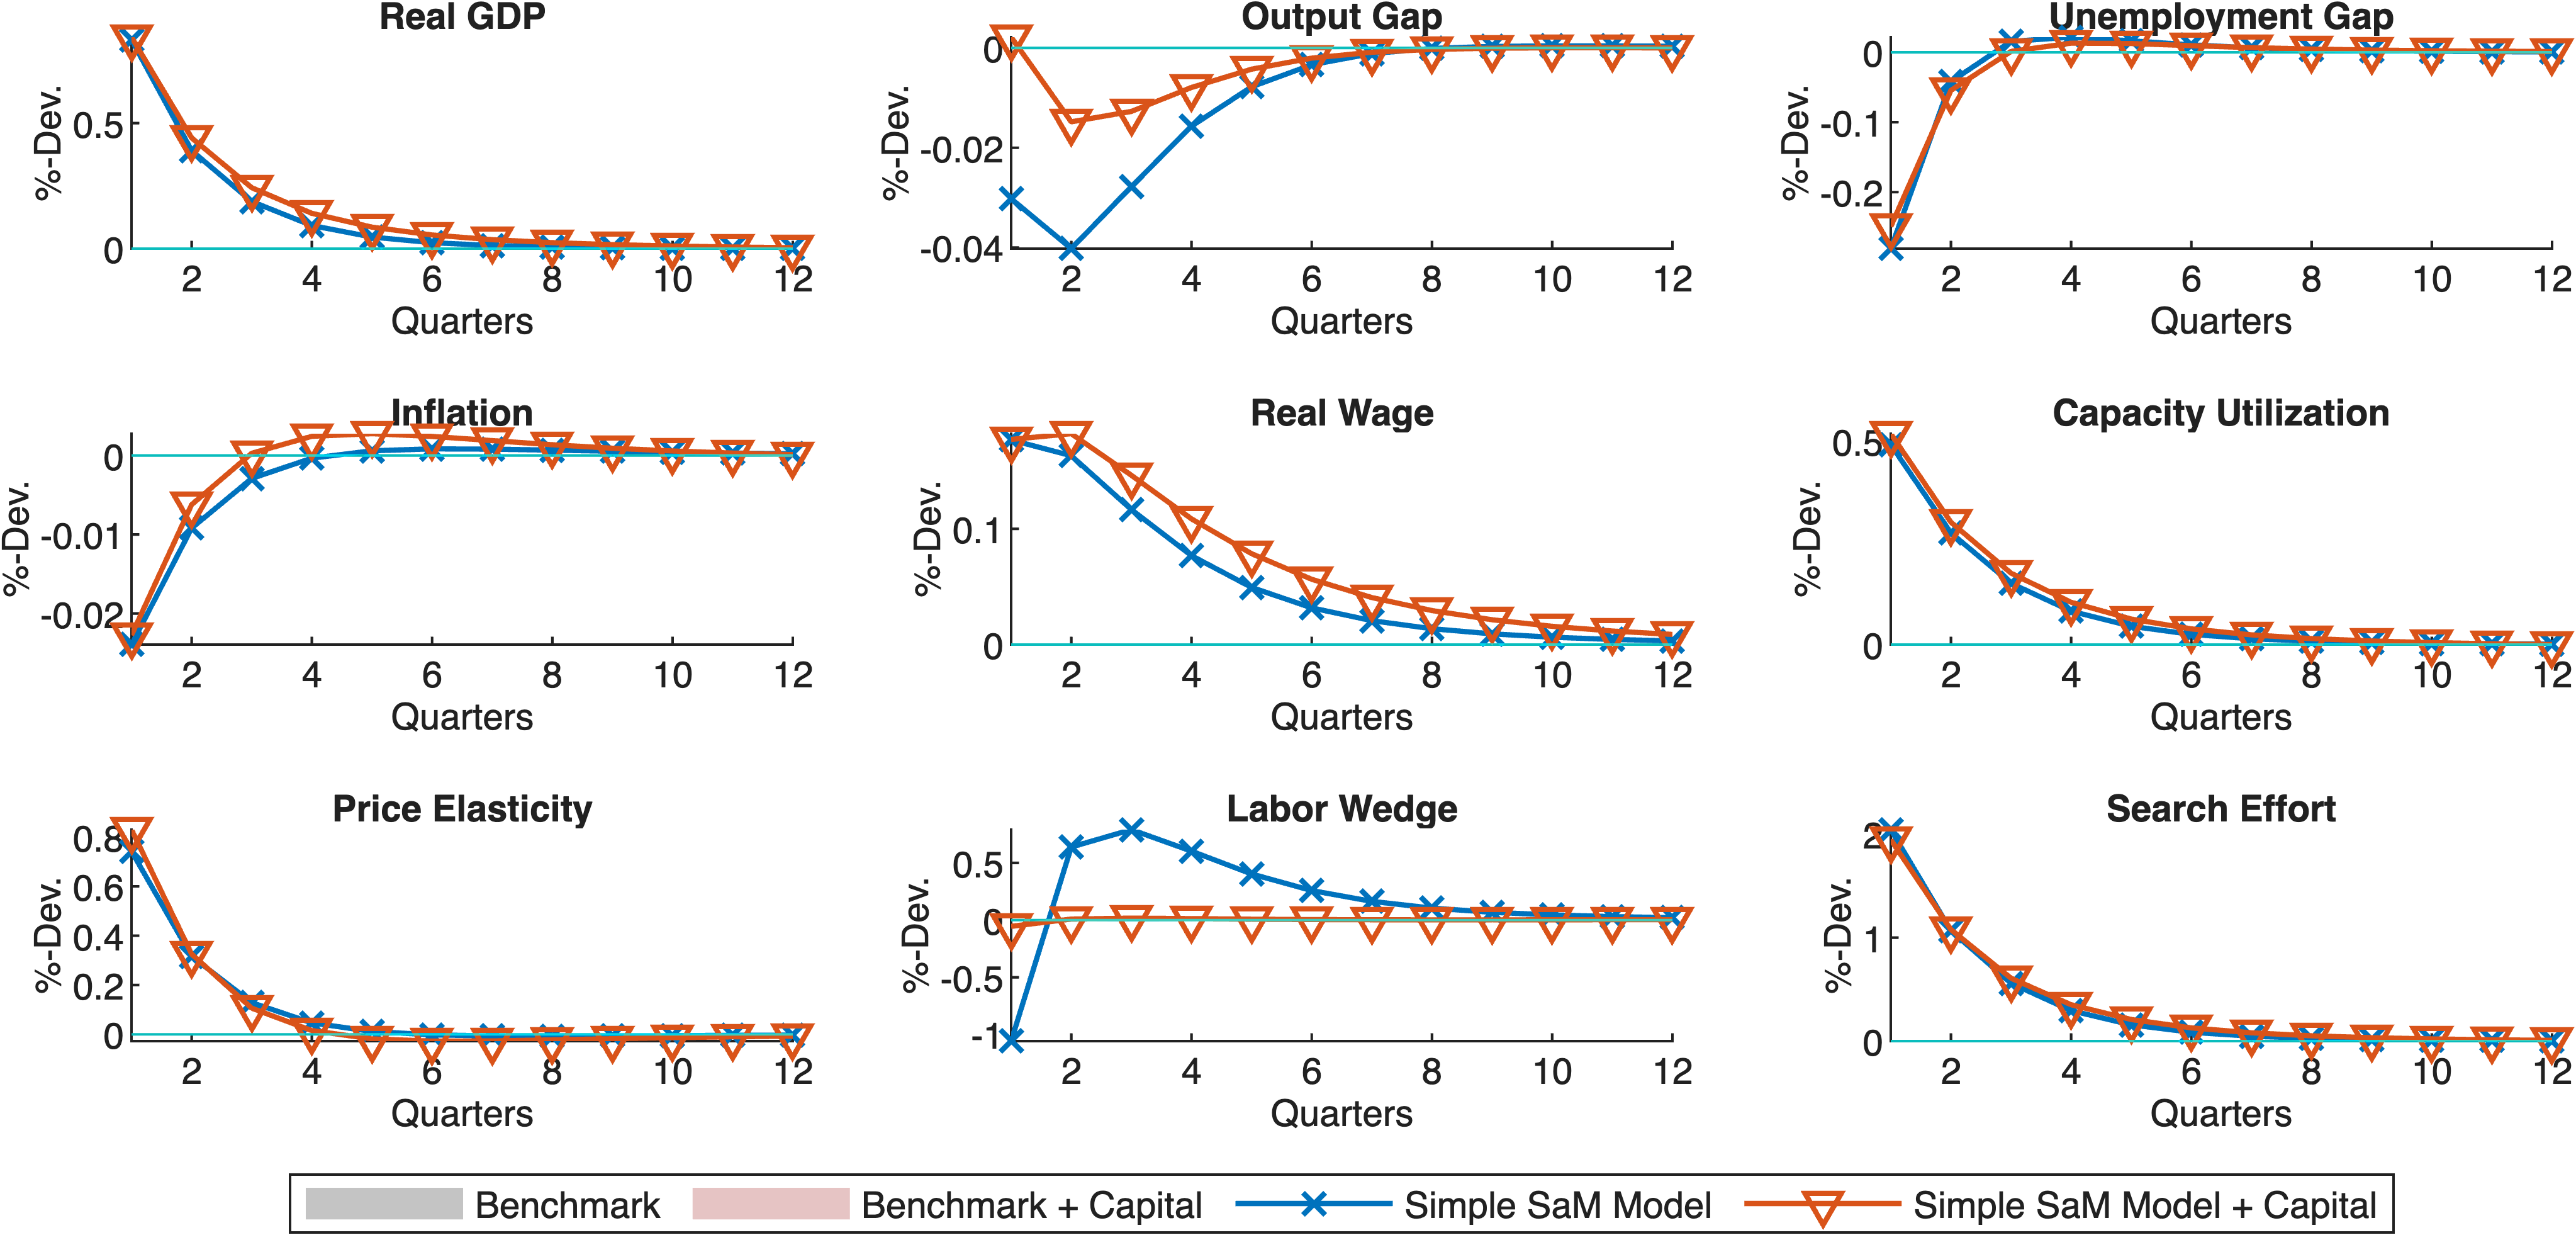
\includegraphics[width=\textwidth]{fig_36_irf_robust_capital_search.png}%
    \end{subfigure}\\%
    {\tiny \singlespacing NOTE: The figure shows IRFs to one standard deviation expansionary shocks using the model presented in \cref{sec:model} and \cref{sec:dynamics}. The benchmark model follows \cref{prop:nosam}, the NK-SaM model is calibrated as in \cref{tab:calibration}. The capital stock and capital utilization channels are added as shown in \ref{sec:full_optimization} and calibrated as in \ref{sec:appendix_calibration}.\par}%
\end{figure}%
% ROBUSTNESS: Long-Term SaM CHANNELS
%-----------------------------------------------------------
\FloatBarrier%
\subsection{Long-Term SaM Channels}\label{sec:robust_longterm_sam}%
% Statistics Table
%--------------------------------------------------------------------------
\begin{table}[h!]%
	\begin{center}%
		\begin{footnotesize}%
			\caption{Inventories and Long-Term Contracts - Relative Standard Deviations and Correlations}\label{tab:app_robust_longterm_sam}%
			\begin{tabular}{l r r r r r r r r}%
				\hline%
				& \multicolumn{2}{c}{TFP} & \multicolumn{2}{c}{Policy} & \multicolumn{2}{c}{Cost-Push} & \multicolumn{2}{c}{Search}\\%
				Variable & Rel.Std. & Corr. & Rel.Std. & Corr. & Rel.Std. & Corr. & Rel.Std. & Corr.\\%
				\hline \hline%
				Output Gap & 0.06 & -0.80 & 1.00 & 1.00 & 0.09 & -0.02 & 0.28 & -0.96\\%
				UE Gap & 0.26 & -0.38 & 1.37 & -0.81 & 1.61 & -0.72 & 0.31 & -0.86\\%
				Inflation & 0.13 & -0.77 & 0.39 & 0.99 & 0.27 & -0.76 & 0.19 & -0.75\\%
				Real Wage & 0.75 & 0.98 & 1.24 & 0.97 & 1.59 & 0.98 & 0.69 & 0.93\\%
				Utilization & 0.49 & -0.46 & 0.51 & -0.04 & 1.05 & -0.53 & 0.56 & 0.99\\%
				Marginal Cost & 0.32 & -0.79 & 1.31 & 0.94 & 2.37 & 0.93 & 0.21 & -0.04\\%
				Price Elasticity & 0.08 & 0.32 & 0.51 & -0.91 & 25.56 & 0.95 & 0.45 & 0.99\\%
				Labor Wedge & 1.27 & 0.88 & 3.22 & -0.76 & 5.95 & -0.79 & 0.29 & -0.19\\%
				Search Effort & 0.57 & -0.19 & 3.10 & 0.88 & 1.01 & -0.95 & 8.06 & 0.90\\%
				\hline%
			\end{tabular}\\%
			\vspace{0.1in}%
			{\tiny NOTE: The table shows simulated second moments for the NK-SaM model. It shows relative standard deviations - standard deviation of each variable relative to standard deviation of real GDP - and correlations of each variable with real GDP. We consider each shock separately in the simulation.\par}%
		\end{footnotesize}%
	\end{center}%
\end{table}%
% IRF Figures - TFP and Demand Shocks
\begin{figure}%
    \centering%
    \caption{Adding Inventories and Long-Term Contracts - IRFs to Expansionary TFP and Demand Shocks}\label{fig:app_irf_robust_longterm_sam_1}%
    \begin{subfigure}{\textwidth}%
        \centering%
        \caption{IRFs to an Expansionary TFP Shock}%
        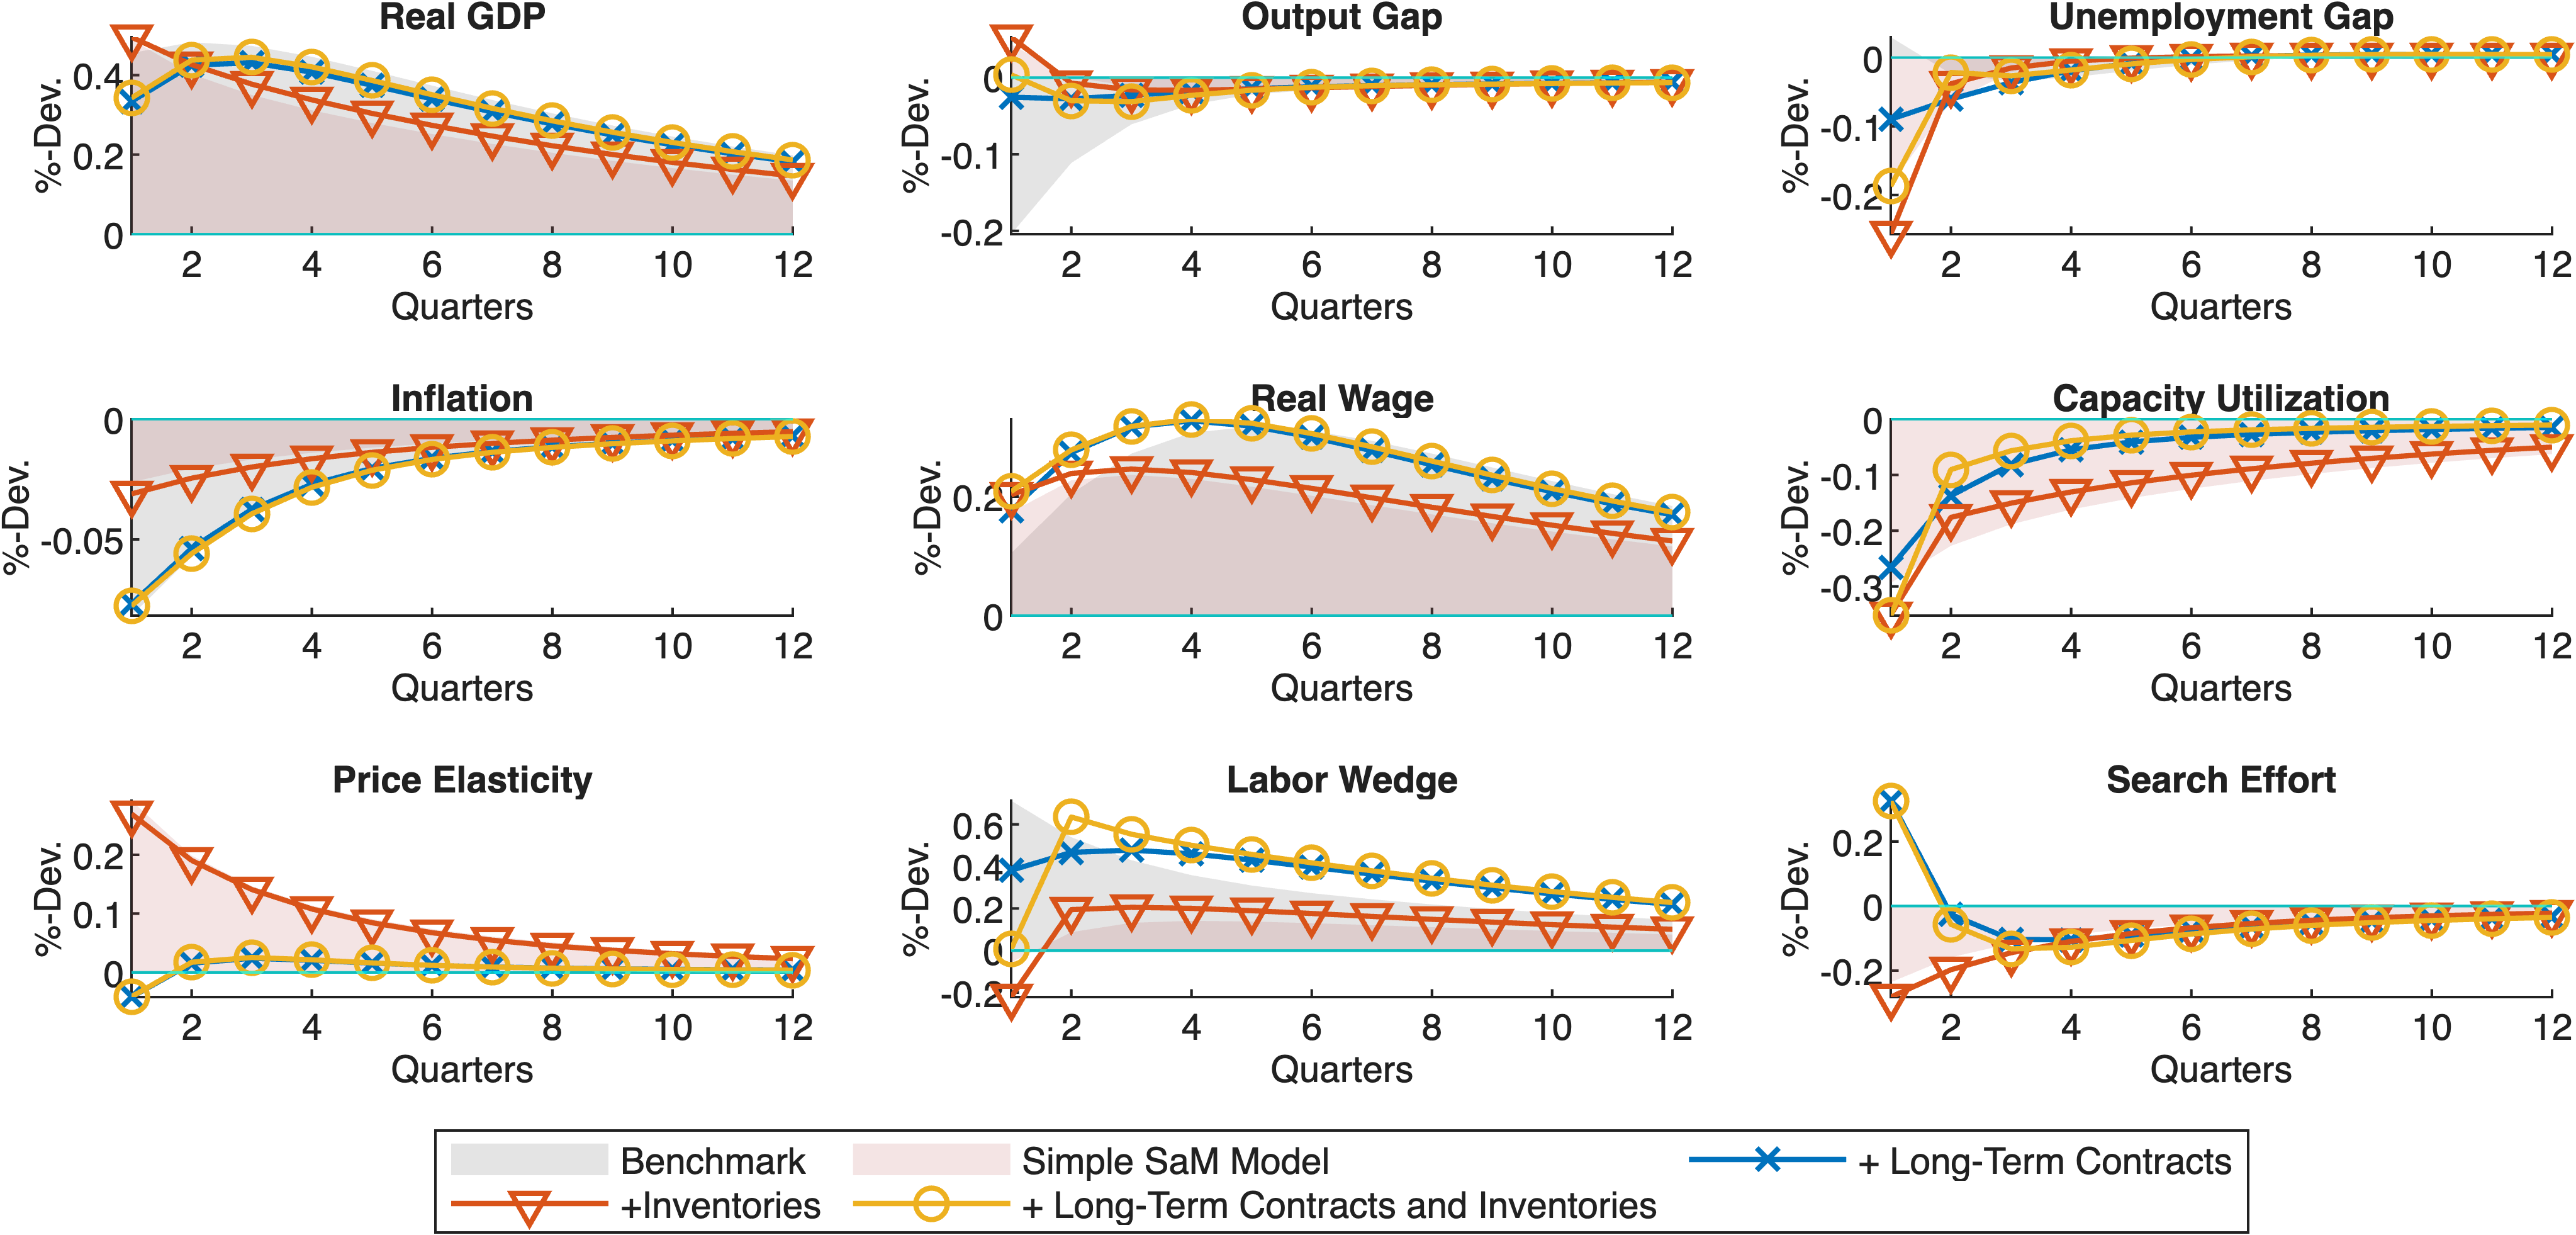
\includegraphics[width=\textwidth]{fig_37_irf_robust_longterm_tfp.png}%
    \end{subfigure}\\%
	\vspace{0.2in}%
    \begin{subfigure}{\textwidth}%
        \centering%
        \caption{IRFs to an Expansionary Monetary Policy Shock}%
        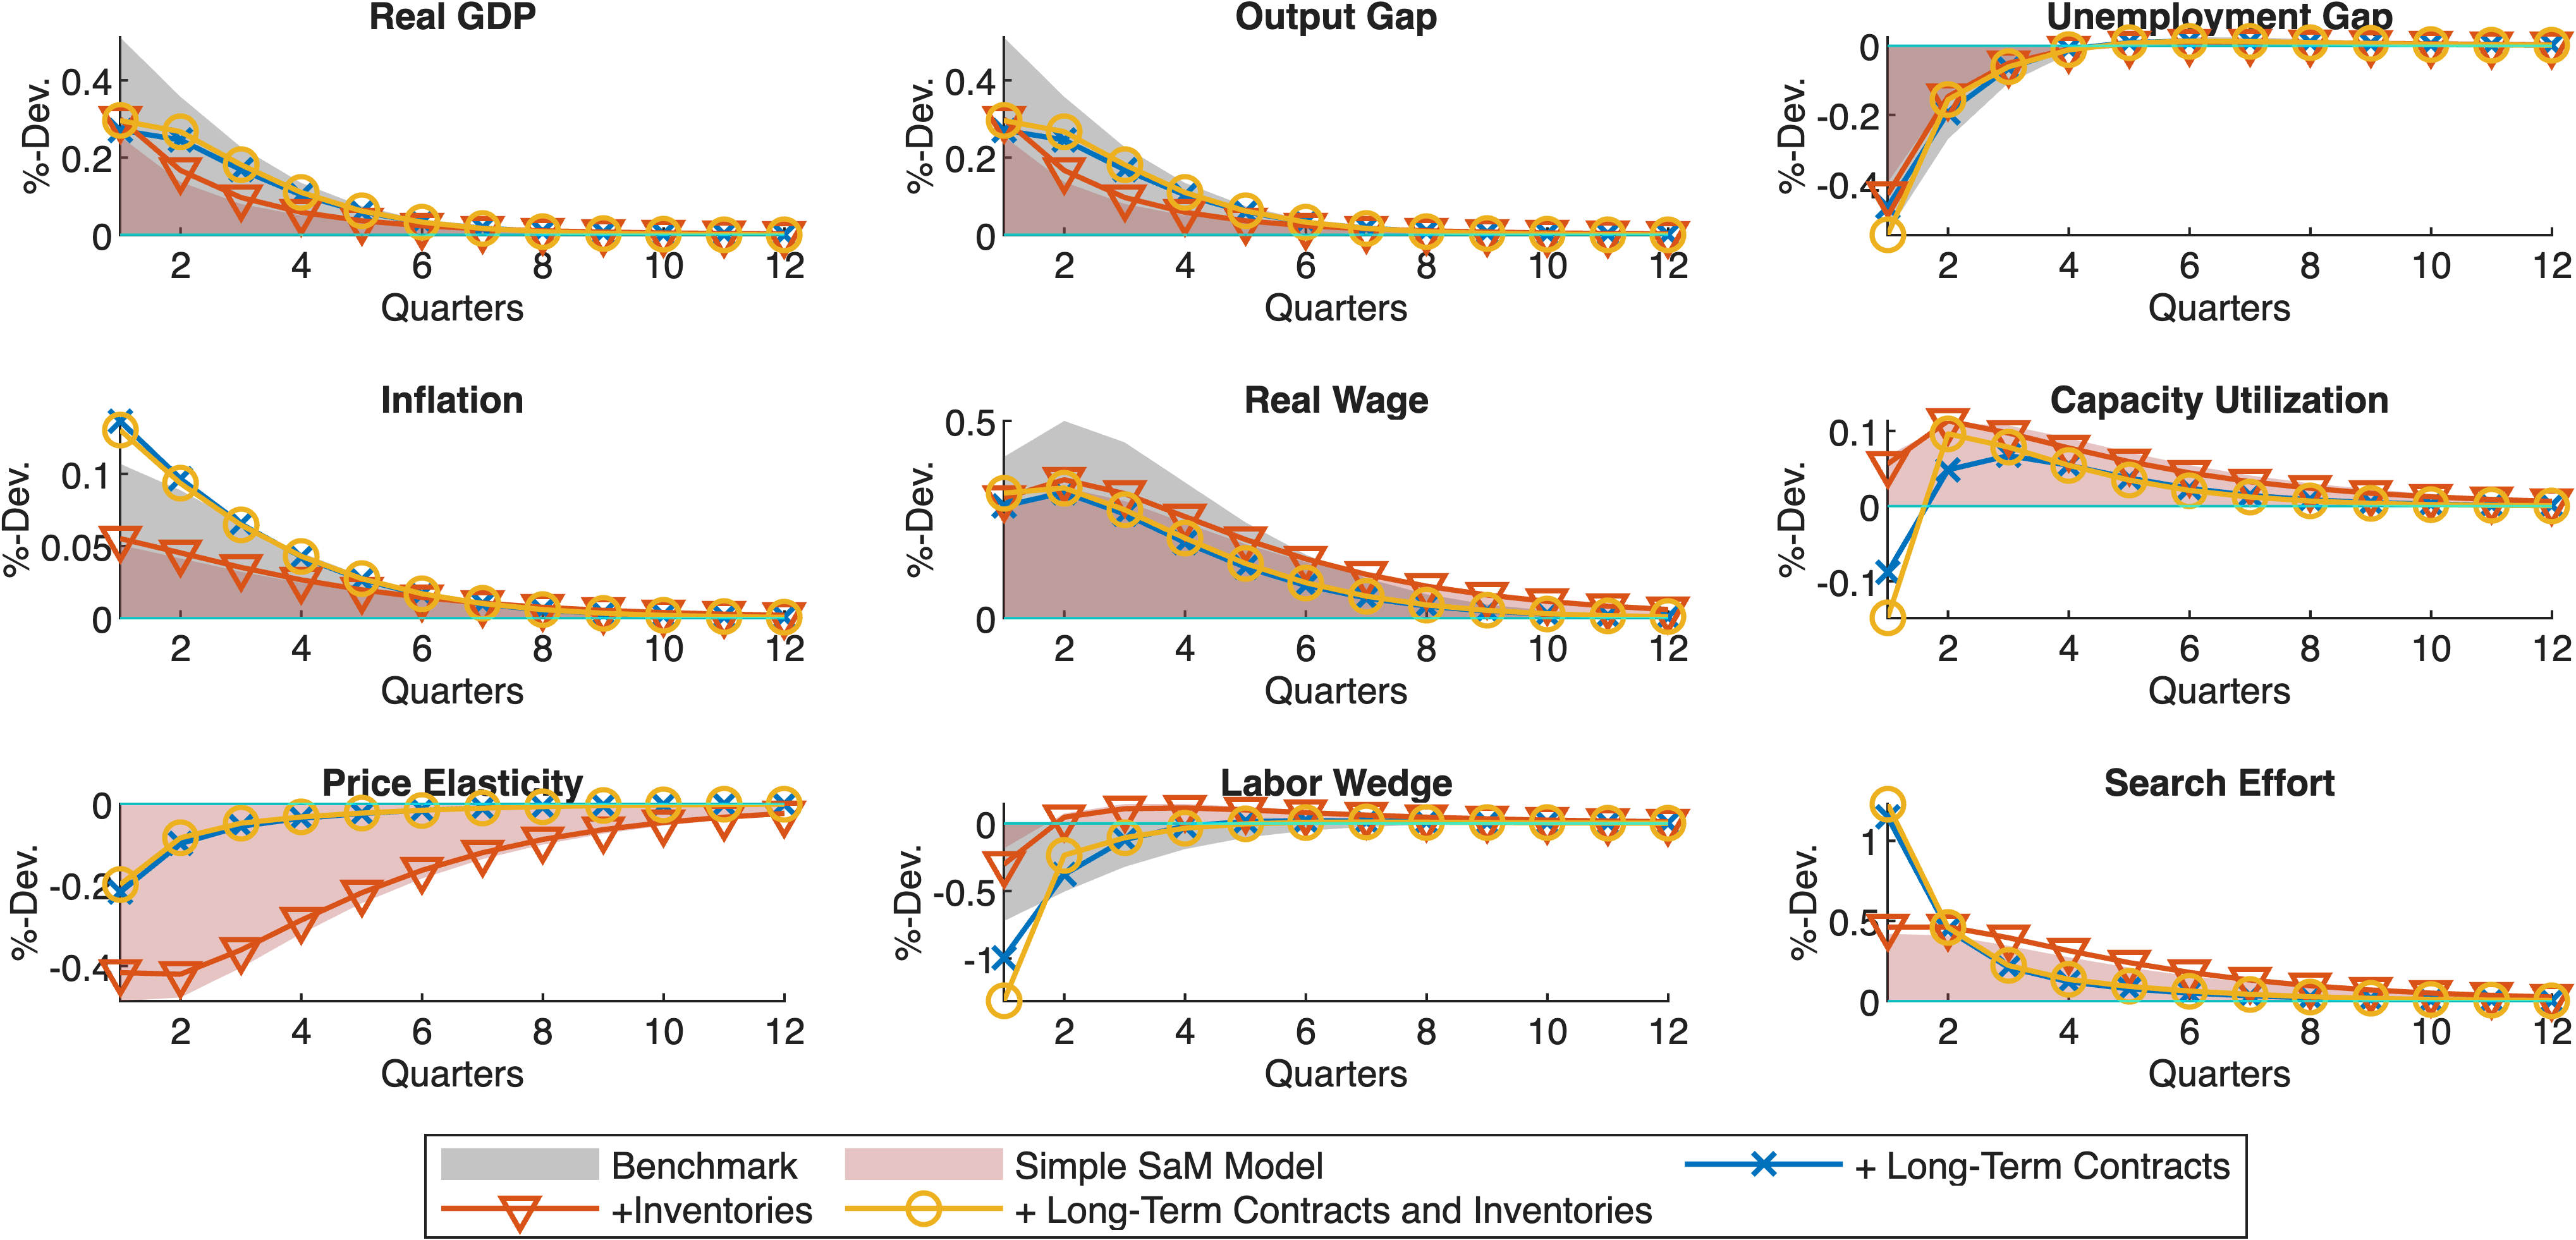
\includegraphics[width=\textwidth]{fig_38_irf_robust_longterm_policy.png}%
    \end{subfigure}\\%
    {\tiny \singlespacing NOTE: The figure shows IRFs to one standard deviation expansionary shocks using the model presented in \cref{sec:model} and \cref{sec:dynamics}. The benchmark model follows \cref{prop:nosam}, the NK-SaM model is calibrated as in \cref{tab:calibration}. The long-term contract and firm inventory channels are added as shown in \ref{sec:full_optimization} and calibrated as in \ref{sec:appendix_calibration}.\par}%
\end{figure}%
% IRF Figures - COST PUSH SHOCKS
\begin{figure}%
    \centering%
    \caption{Adding Inventories and Long-Term Contracts - IRFs to Expansionary Cost Push Shocks}\label{fig:app_irf_robust_longterm_sam_2}%
    \begin{subfigure}{\textwidth}%
        \centering%
        \caption{IRFs to an Expansionary EIS Shock}%
        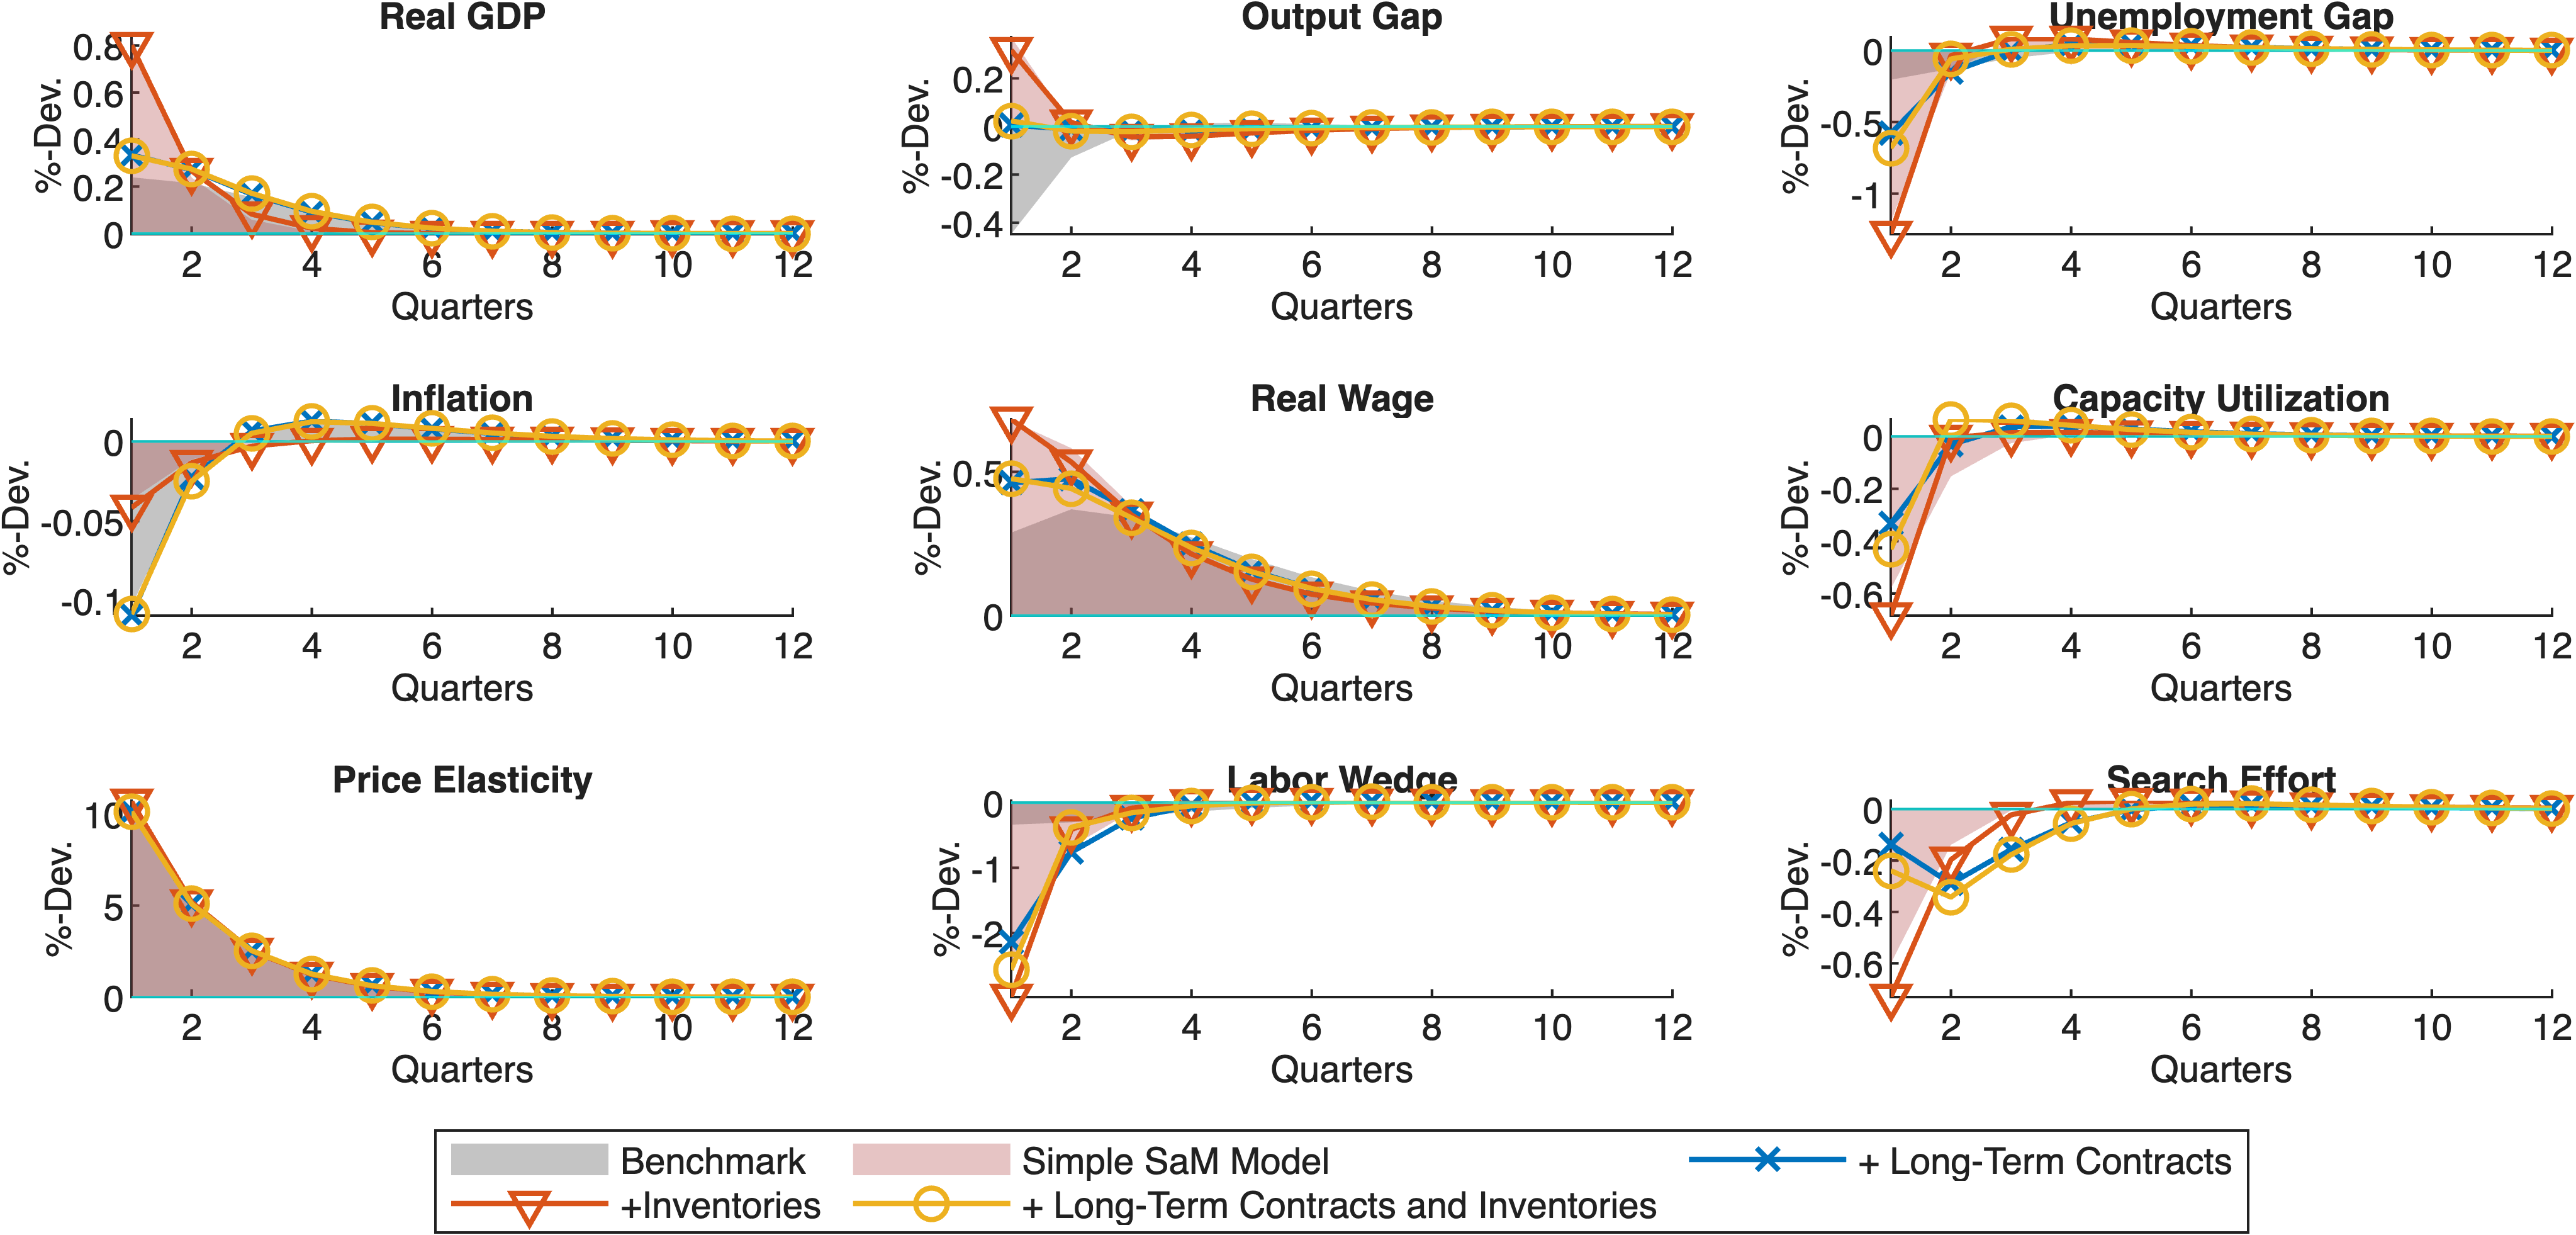
\includegraphics[width=\textwidth]{fig_39_irf_robust_longterm_eis.png}%
    \end{subfigure}\\%
	\vspace{0.2in}%
    \begin{subfigure}{\textwidth}%
        \centering%
        \caption{IRFs to an Expansionary Search Effort Shock}%
        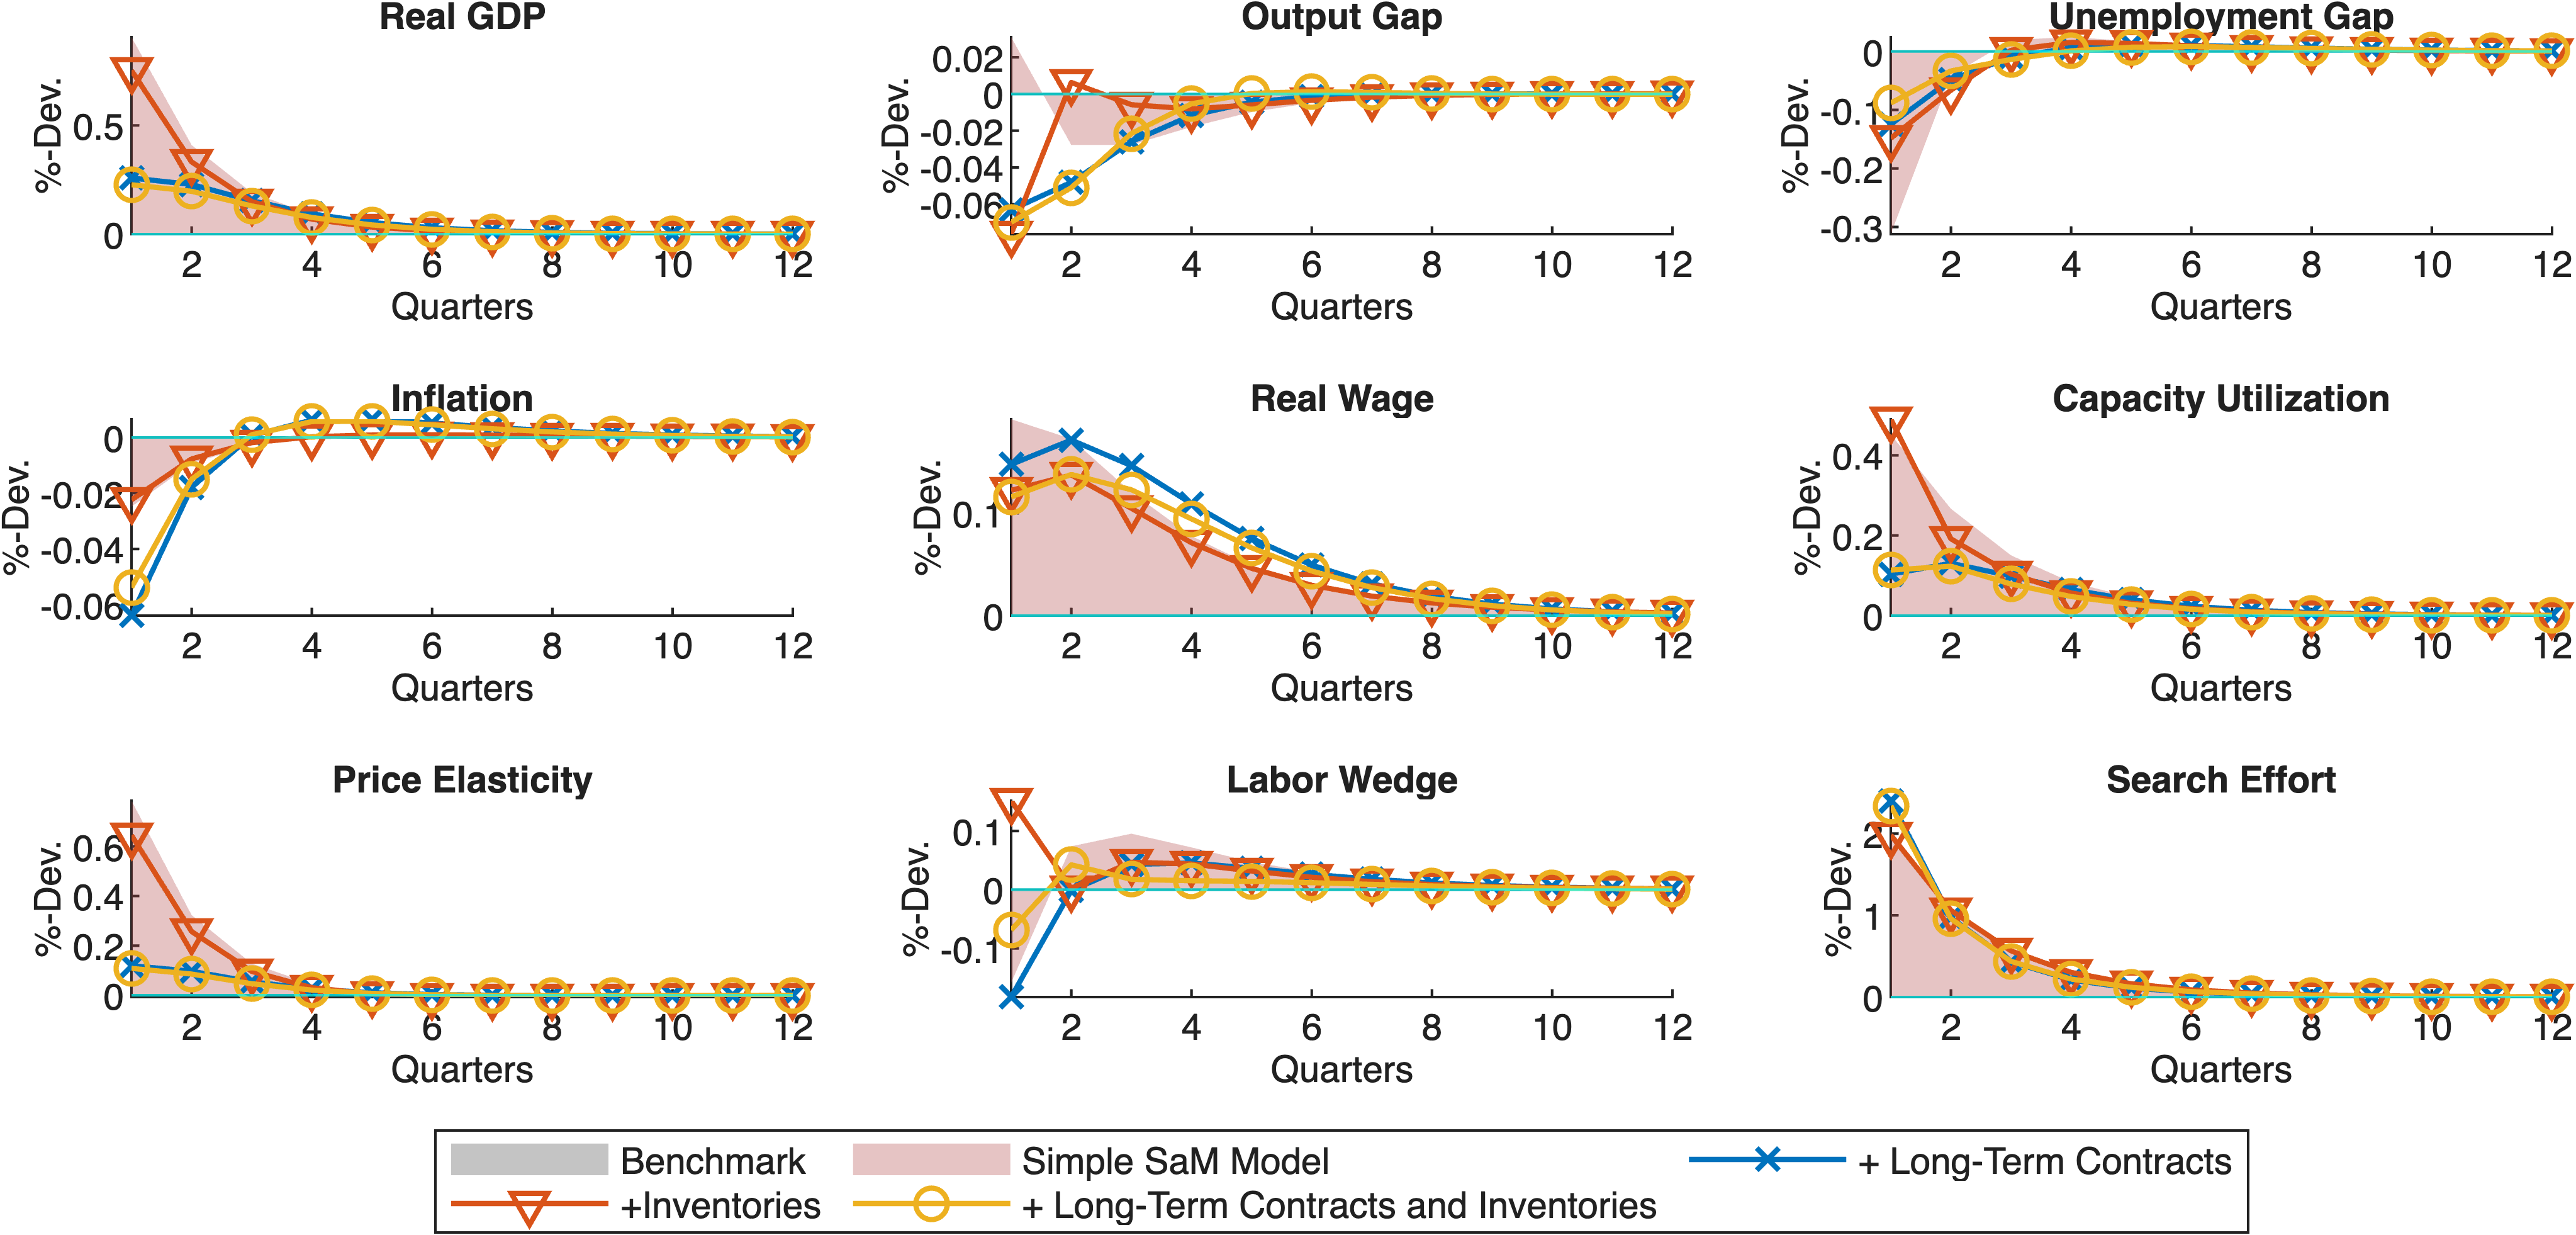
\includegraphics[width=\textwidth]{fig_40_irf_robust_longterm_search.png}%
    \end{subfigure}\\%
    {\tiny \singlespacing NOTE: The figure shows IRFs to one standard deviation expansionary shocks using the model presented in \cref{sec:model} and \cref{sec:dynamics}. The benchmark model follows \cref{prop:nosam}, the NK-SaM model is calibrated as in \cref{tab:calibration}. The long-term contract and firm inventory channels are added as shown in \ref{sec:full_optimization} and calibrated as in \ref{sec:appendix_calibration}.\par}%
\end{figure}%
%--------------------------------------------------------------------------
% END OF THE DOCUMENT
%--------------------------------------------------------------------------
\end{document}%